%:Clase del documento

\documentclass[fontsize=10pt, Myfinal=true, English=true, twoside, numbers=noenddot]{scrbook}
%Minion=true, English=true, Myfinal=true

\makeatletter
\let\alloc@latex\alloc@
\def\alloc@#1#2#3#4{\newcount}% the current \newcount doesn't use \alloc@
\makeatother


%:Paquete de estilos propuesto
\usepackage{libroETSI}
%:Paquete específico para cargar tikz (y sus librerías) y pgfplots
\usepackage{dtsc-creafig}
%:Paquete para notaciones específicas
\usepackage{notacion}
%:Paquete para incorporar aspectos concretos de la edición
\usepackage{edicionPFC}

\usepackage[table,xcdraw]{xcolor}




\makeatletter
\let\alloc@\alloc@latex
\makeatother


%:Estas líneas de código son INNECESARIAS excepto para mostrar determinadas características en este manual. Pueden eliminarse o comentarse sin ningún problema.
%Se usan para compilar el capítulo estilolibroetsi.tex
\usepackage[final]{showexpl}
\lstset{explpreset={frame=none,rframe={}, numbers=none,numbersep=3pt, columns=flexible,language={[LaTeX]TeX},basicstyle=\ttfamily,keywordstyle=\color{blue}}}%numberstyle=\tiny,

%:Para modificar fácilmente la fuente del texto.
\makeatletter
\ifdtsc@Minion % Queremos utilizar la fuente Minion y lo hemos declarado al principio
	\ifluatex
		\setmainfon$•$t[Renderer=Basic, Ligatures=TeX,	% Fuente del texto 
		Scale=1.01,
		]{Minion Pro}
   		% En este caso conviene modificar ligeramente el tamaño de las fuentes matemáticas
		\DeclareMathSizes{10}{10.5}{7.35}{5.25}
		\DeclareMathSizes{10.95}{11.55}{8.08}{5.77}
		\DeclareMathSizes{12}{12.6}{8.82}{6.3}
%		\setmainfont[Renderer=Basic, Ligatures=TeX,	% Fuente del texto 
%		]{Adobe Garamond Pro}
%		\setmainfont[Renderer=Basic, Ligatures=TeX,	% Fuente del texto 
%		]{Palatino LT Std}
	\fi
\else
	\ifluatex
		% Para utilizar la fuente Times New Roman, o alguna otra que se tenga instalada
		\setmainfont[Renderer=Basic, Ligatures=TeX,	% Fuente del texto 
		Scale=1.0,
		]{Times New Roman}
	\else
		\usepackage{tgtermes} 	%clone of Times
		%\usepackage[default]{droidserif}
		%\usepackage{anttor} 	
	\fi
\fi
\makeatother

%Por si quieren usar bibliografía con BIBER
%BIBER%%:Para la bibliografía en BIBER, descomentar las líneas siguientes
%\defbibheading{etsi}[]{%
%	\chapter*{Bibliografía}%
%	\chaptermark{Bibliografía} 
%	\markboth{#1}{#1}}
%\addbibresource{bibliografiaLibroETSI.bib}

% Ejemplo de Glosario
\newacronym[type=main]{ETSI}{ETSI}{Escuela Técnica Superior de Ingeniería}
\newacronym[type=main]{US}{US}{Universidad de Sevilla}
\newacronym[type=main]{DMC}{DMC}{Canal Discreto sin Memoria}


\makeindex
\makeglossaries %Si no se quiere el glosario, comentar esta línea.

% Formato A4
\geometry
{paperheight=297mm,%
paperwidth=210mm,%
top=25mm,%
headsep=8.5mm,%
includefoot, 
textheight=240mm, 
textwidth=150mm, 
bindingoffset=0mm, 
twoside}

\usepackage[a4,center]{crop}%para poner las cruces de esquina de página, poner la opción cross

%:Esquema de numeración por defecto
\setenumerate[1]{label=\normalfont\bfseries{\arabic*.}, leftmargin=*, labelindent=\parindent}
\setenumerate[2]{label=\normalfont\bfseries{\alph*}), leftmargin=*}
\setenumerate[3]{label=\normalfont\bfseries{\roman*.}, leftmargin=*}
\setlist{itemsep=.1em}
\setlength{\parindent}{1.0 em}

\setcounter{tocdepth}{4}						% El nivel hasta el que se muestra el índice 


%:Empieza el documento

\begin{document}
%:Para incluir toda la referencia bibliográfica aunque no se cite, descomente la siguiente línea
%\nocite{*}


%PORTADA
%ver edicionPFC.sty para modificaciones

%:Para crear la portada y la portada interior (pagina titular) 
\titulo{Time Series Forecasting Using Transformer-based Models: Exploring Transformer, Informer, and Autoformer} %\mbox evita que se divida una palabra al cambiar de línea
\autor{Antonio Luis González Hernández}
\director{Juan Antonio Becerra González}
\titulodirector{Profesor Titular}

\departamento{Dpto. Teoría de la Señal y  Comunicaciones}
\centro{Escuela Técnica Superior de Ingeniería}
\universidad{Universidad de Sevilla}
\titulacion{Ingeniería Electrónica, Robótica y Mecatrónica}
\fecha{2024}
\nombretrabajo{Trabajo Fin de Grado} %Trabajo Fin de Grado, Proyecto fin de Máster,....

\hypersetup
{
	linkcolor=black, %Tocar para poner color en enlaces
	pdfauthor={\elautor},
	pdftitle={\nombretrabajo,\eltitulo},
	pdfkeywords={Latex, edición, formato de texto}
}

\portadaPFC{figuras/LogoUS.pdf}{figuras/LogoTSC.pdf} %logo de la Universidad y logo del departamento, si lo hubiera. Para cambiar el pie de página con los logos, debe editarse el fichero ediciónPFC.sty

%Fin Portada

%:Todo lo que constituye la primera parte del libro que no es el cuerpo del libro en realidad
\frontmatter
\pagenumbering{Roman} %Pone la numeración en mayúscula (En español parece que es obligatorio)


%% !TEX root =../LibroTipoETSI.tex
\chapter*{Agradecimientos}
%\pagestyle{especial}
\pagestyle{empty}
%\chaptermark{Agradecimientos}
\phantomsection
%\addcontentsline{toc}{listasf}{Agradecimientos}
%\vspace{1cm}
%{\huge{Agradecimientos}}
%\vspace{1cm}

\lettrine[lraise=-0.1, lines=2, loversize=0.25]{E}{l} diseño de una hoja de estilo en \LaTeX\ para un texto no es en absoluto trivial. Por un lado hay que conocer bien los usos, costumbres y reglas que se emplean a la hora de establecer márgenes, tipos de letras, tamaños de las mismas, títulos, estilos de tablas, y un sinfín de otros aspectos. Por otro, la programación en \LaTeX\ de esta hoja de estilo es muy tediosa, incluida la selección de los mejores paquetes para ello. La hoja de estilo adoptada por nuestra Escuela y utilizada en este texto es una versión de la que el profesor Payán realizó para un libro que desde hace tiempo viene escribiendo para su asignatura. Además, el prof. Payán ha participado de forma decisiva en la adaptación de dicha plantilla a los tres tipos de documentos que se han tenido en cuenta: libro, tesis y proyectos final de carrera, grado o máster. Y también en la redacción de este texto, que sirve de manual para la utilización de estos estilos. Por todo ello, y por hacerlo de forma totalmente desinteresada, la Escuela le está enormemente agradecida.

A esta hoja de estilos se le incluyó unos nuevos diseños de portada. El diseño gráfico de las portadas para proyectos fin de grado, carrera y máster, está basado en el que el prof. Fernando García García, de la Facultad de Bellas Artes de nuestra Universidad, hiciera para los libros, o tesis, de la sección de publicación de nuestra Escuela. Nuestra Escuela le agradece que pusiera su arte y su trabajo, de forma gratuita, a nuestra disposición.

%gradecemos}, a todos nuestros maestros, cuanto nos enseñaron.

{\flushleft{\hfill \emph{Juan José Murillo Fuentes}}}%
\vspace{-.3cm}
{\flushleft{\hfill \emph{Subdirección de Comunicaciones y Recursos Comunes}}}%
{\flushleft{\hfill \emph{Seville, 2013}}}%

 
%% !TEX root =../LibroTipoETSI.tex
\chapter*{Resumen}
\pagestyle{especial}
\chaptermark{Resumen}
\phantomsection
\addcontentsline{toc}{listasf}{Resumen}

\lettrine[lraise=-0.1, lines=2, loversize=0.2]{E}{s}te Trabajo de Fin de Grado explora la aplicación de arquitecturas Transformer a la predicción de series temporales, examinando específicamente los modelos Transformer, Informer y Autoformer. La predicción de series temporales es un área crucial con aplicaciones en finanzas, meteorología, agricultura y más, que implica la predicción de valores futuros basándose en datos históricos.

La investigación examina la arquitectura Transformer, que se desarrolló originalmente para el procesamiento de lenguaje natural, y evalúa su potencial en la predicción de datos de series temporales. Al extender trabajos previos que emplearon enfoques estadísticos y de redes neuronales para predecir variaciones en el diámetro de plantas, este estudio busca evaluar cómo los modelos Transformer pueden mejorar las capacidades de predicción, particularmente en series de tiempo multivariadas.

El estudio comienza con una visión histórica de los métodos de predicción de series temporales, detallando la evolución desde los enfoques tradicionales hasta los modernos, y destacando los avances recientes en arquitecturas de aprendizaje automático. Luego, proporciona un examen detallado de la arquitectura Transformer, incluidos sus componentes clave y su adaptación para la predicción de series temporales. También se discuten variantes como Informer y Autoformer, con un enfoque en sus contribuciones y mejoras específicas.

La metodología de investigación incluye un análisis exhaustivo de los conjuntos de datos utilizados, los pasos de preprocesamiento realizados y el diseño experimental, que involucra la optimización de hiperparámetros y la evaluación del rendimiento. Los resultados se presentan en términos de la efectividad de los modelos basados en Transformer bajo diversas configuraciones, proporcionando información sobre su rendimiento y ventajas potenciales.

En general, este trabajo contribuye a la comprensión de los modelos Transformer en el contexto de la predicción de series temporales, ofreciendo una evaluación detallada de su eficacia y limitaciones. Los hallazgos buscan informar sobre futuras direcciones de investigación y aplicaciones prácticas, particularmente en la optimización de arquitecturas Transformer para tareas complejas de predicción.

%La hoja de estilo utilizada es una versión de la que el Prof. Payán realizó para un libro que desde hace tiempo viene escribiendo para su asignatura. Con ella se han realizado estas notas, a modo de instrucciones, añadiéndole el diseño de la portada. El diseño de la portada está basado en el que el prof. Fernando García García, de nuestra universidad, hiciera para los libros de la sección de publicación de nuestra Escuela.


\chapter*{Abstract}
\pagestyle{especial}
\chaptermark{Abstract}
\phantomsection
\addcontentsline{toc}{listasf}{Abstract}

\lettrine[lraise=-0.1, lines=2, loversize=0.2]{T}{h}is Final Degree Project explores the application of Transformer architectures to time series forecasting, specifically examining the Transformer, Informer, and Autoformer models. Time series forecasting is a crucial area with applications spanning finance, meteorology, agriculture, and more, involving the prediction of future values based on historical data.

The research investigates the Transformer architecture, which was originally developed for natural language processing, and evaluates its potential in forecasting time series data. By extending previous work that employed statistical and neural network approaches to predict plant diameter variations, this study aims to assess how Transformer models can enhance forecasting capabilities, particularly in both univariate and multivariate contexts.

The study begins with a historical overview of time series forecasting methods, detailing the evolution from traditional to modern approaches and highlighting recent advancements in machine learning architectures. It then provides an in-depth examination of the Transformer architecture, including its core components and its adaptation for time series forecasting. Variants such as Informer and Autoformer are also discussed, with a focus on their specific contributions and improvements.

The research methodology includes a comprehensive analysis of the datasets used, the preprocessing steps undertaken, and the experimental design, which involves hyperparameter tuning and performance evaluation. The results are presented in terms of the effectiveness of the Transformer-based models under various configurations, providing insights into their performance and potential advantages.

Overall, this work contributes to the understanding of Transformer models in the context of time series forecasting, offering a detailed evaluation of their efficacy and limitations. The findings aim to inform future research directions and practical applications, particularly in optimizing Transformer architectures for complex forecasting tasks.

 

% Índice abreviado 
% El índice abreviado se incluye también en algunos libros, con menor detalle que el completo. Descomentar las siguientes líneas.
\cleardoublepage
\phantomsection
\addcontentsline{toc}{listasf}{Índice Abreviado}
\pagestyle{especial}
\shorttoc{Índice Abreviado}{1}

%Índice normal, el completo
\cleardoublepage
\phantomsection
\pagestyle{especial}
\tableofcontents


%\chapter*{\notationname}
\pagestyle{especial}
\chaptermark{\notationname}
\phantomsection
\addcontentsline{toc}{listasf}{\notationname}
%\section*{Notación}
%\begin{table}[htbp]
\begin{longtable}{p{3cm}p{8.5cm}}

%$\displaystyle D$ & Tasa de símbolos  (sim/s) \\
%$\displaystyle R_b$ & Tasa binaria (bit/s) \\
%$\displaystyle T$ & Tiempo de símbolo (s) \\
%$\displaystyle T_{b}$ & Tiempo de bit (s) \\
%$W\left( {t} \right)$ & Ruido blanco\\
%$w\left( {t} \right)$ & Función muestra de un ruido blanco\\
%$\displaystyle h_{c}\left( {t} \right)$ & Respuesta impulsiva de un canal LTI continuo en el tiempo\\
%$\displaystyle H_{c}\left( {\omega} \right)$ & Respuesta en frecuencia de un canal LTI continuo en el tiempo\\
%$\displaystyle h_{c}\left( {\tau;t} \right)$ & Respuesta impulsiva de un canal LTV continuo en el tiempo\\
%$\displaystyle H_{c}\left( {\omega;t} \right)$ & Respuesta en frecuencia de un canal LTV continuo en el tiempo\\
%$\displaystyle h_{c}\left( {n} \right)$ & Respuesta impulsiva de un canal LTI discreto en el tiempo\\
%$\displaystyle H_{c}\left( {\Omega} \right)$ & Respuesta en frecuencia de un canal LTI discreto en el tiempo\\
$\RR$ & Cuerpo de los números reales \\
$\CC$ & Cuerpo de los números complejos\\
$\left\| \vc{v} \right\|$ & Norma del vector $\vc{v}$ \\
$\left\langle {\vc{v}, \vc{w}} \right\rangle$ & Producto escalar de los vectores $\vc{v}$ y $\vc{w}$\\
$\left| {\vc{A}} \right|$ &Determinante de la matriz cuadrada $\vc{A}$\\
$\textrm{det}\left( {\vc{A}} \right)$ &Determinante de la matriz (cuadrada) $\vc{A}$\\
$\vc{A}\trs$ & Transpuesto de $\vc{A}$\\
$\vc{A}\inv$ & Inversa de la matriz $\vc{A}$\\
$\vc{A}{\psd}$ & Matriz pseudoinversa de la matriz $\vc{A}$\\
$\vc{A}\her$ & Transpuesto  y conjugado de $\vc{A}$\\
$\vc{A}\cnj$ & Conjugado\\
c.t.p. & En casi todos los puntos\\
c.q.d. & Como queríamos demostrar\\
\ensuremath{\blacksquare}& Como queríamos demostrar\\
\ensuremath{\square}& Fin de la solución\\
e.o.c. & En cualquier otro caso\\
$\e$ & número e\\
$\xp{x}$ & Exponencial compleja\\
$\xppi{x}$ & Exponencial compleja con $2\pi$\\
$\nxp{x}$ & Exponencial compleja negativa\\
$\nxppi{x}$ & Exponencial compleja negativa con $2\pi$\\
$\re$ & Parte real\\
$\im$ & Parte imaginaria\\
$\sen$ & Función seno \\
$\tg$ & Función tangente \\
$\arctg$ & Función arco tangente \\
$\sento{y}{x}$ & Función seno de $x$  elevado a $y$\\
$\costo{y}{x}$ & Función coseno de $x$  elevado a $y$\\
$\sa$ & Función sampling \\
$\sgn$ & Función signo \\
$\rect$ & Función rectángulo \\
$\sinc$ & Función sinc\\
$\pder{y}{x} $ & Derivada parcial de $y$ respecto a $x$\\
$x\gra$ & Notación de grado, $x$ grados.\\
%
%$C_{XY}$& covarianza  de dos variables aleatorias reales $X$ e $Y$\\
%$R_{XY}$& correlación  de dos variables aleatorias reales $X$ e $Y$\\
%$\rho_{XY}$ &Coeficiente de correlación de las variables aleatorias reales $X$  e $Y$\\
%$\vc{Z}$ & Vector aleatorio complejo\\
%$\displaystyle F_{X}\left( {\cdot} \right)$ & Función de distribución de la variable aleatoria $X$ \\
%$\displaystyle f_{X}\left( {\cdot} \right)$ & Función densidad de probabilidad de la variable aleatoria $X$ \\
%$p_{X}\left( {\cdot} \right)$ & Función masa de probabilidad de la variable aleatoria discreta $X$ \\
%
$\Pr\left( {A} \right)$ & Probabilidad del suceso $A$ \\
$\displaystyle E\left[ {X} \right]$ & Valor esperado de la variable aleatoria $X$ \\
$\si{X}$ & Varianza de la variable aleatoria $X$\\
$\sim f_{X}\left( {x} \right)$ & Distribuido siguiendo la función densidad de probabilidad $f_{X}\left( {x} \right)$\\
%
$\gauss{m_{X}}{\si{X}}$ &Distribución gaussiana para la variable aleatoria X, de media $m_{X}$ y varianza $\si{X}$ \\
$\id{n}$ & Matriz identidad de dimensión $n$\\
$\diag{\vc{x}}$ & Matriz diagonal a partir del vector $\vc{x}$\\
$\diag{\vc{A}}$ & Vector diagonal de la matriz $\vc{A}$\\
$\snr$& Signal-to-noise ratio \\
$\mse$ & Minimum square error\\
$\talq$ & Tal que \\
$\eqdef$ & Igual por definición \\
$\norm{\vc{x}}$ & Norma-2 del vector $\vc{x}$\\
$\card{\vc{{A}}}$ & Cardinal, número de elementos del conjunto $\vc{A}$\\
$\xyz{\vc{x}}{i}{n}$ & Elementos $i$, de 1 a $n$, del vector $\vc{x}$\\
%\newcommand{\xyz}[3]{\ensuremath{#1_{#2},#2=1,2,\ldots,#3}}
$\df{x}$& Diferencial de $x$\\
$\le$ & Menor o igual \\
$\ge$ & Mayor o igual \\
$\BL$ & Backslash \\
$\iff$ & Si y sólo si \\
$x=a+3\eqexpl{a=1} 4 $& Igual con explicación \\
$\tfrac{a}{b}$ & Fracción con estilo pequeño, $a/b$ \\
$\inc$ & Incremento \\
$b\ten{a}$ & Formato científico \\
$\tendsub{x}$ & Tiende, con x \\
$\ord$ & Orden\\
$\tm$ & Trade Mark\\
$\E[x]$ & Esperanza matemática de x\\
$\covm{\vc{x}}$ & Matriz de covarianza de $\vc{x}$\\
$\corrm{\vc{x}}$ & Matriz de correlación de $\vc{x}$\\
$\si{x}$ & Varianza de x \\


\end{longtable}
\newpage
%\end{table}
%


%\phantomsection
%\addcontentsline{toc}{listasf}{Acrónimos}
%\section*{Acrónimos}
%\begin{table}[htbp]
%\begin{tabular}{p{2cm}p{10cm}}
%Escuela Técnica Superior de In
%LTI & Lineal Invariante con el Tiempo \\
%LTV& Lineal Variable con el Tiempo\\
%AWGN& Ruido blanco gaussiano aditivo\\
%DMS& Fuente discreta sin memoria\\
%AEP& Propiedad de equipartición asintótica\\
%WLLN& Ley Débil de los Grandes Números\\
%DMC& Canal Discreto sin Memoria\\
%BSC& Canal Simétrico Binario\\
%BEC& Canal Binario con Borrado\\
%\end{tabular}
%\end{table}


%\nota{El libro de Lapidoth tiene una excelente recopilación.} %No incluir si no se quiere, comentándolo

%:Empieza el contenido del libro
\mainmatter

%:Página por defecto
\pagestyle{esitscCD}

%:Los diferentes capítulos, en carpetas separadas
\chapter{Introduction}\LABCHAP{CAP1}
\pagestyle{esitscCD}

Time series forecasting is a critical area of research with broad applications across numerous domains, including finance, meteorology, and agriculture. At its core, time series forecasting involves predicting future values based on previously observed data points collected over time. This process is essential for making informed decisions and planning, particularly in contexts where temporal dynamics play a crucial role.

This dissertation builds upon a series of previous research projects that focused on forecasting plant diameter variations. The foundational work by Paula Fernández Yepes\cite{FernandezYepes2022} employed statistical methods to model the growth of plant diameter, while Andrés Benítez González\cite{BenitezGonzalez2023} expanded on this by utilizing neural network models to predict variations in plant diameter. The primary objective of these studies was not merely to track growth but to anticipate changes in diameter variation that could signal plant health issues, such as disease.

In pursuit of advancing this research, the present study explores the application of the Transformer architecture for time series forecasting. The choice of the Transformer model was motivated by its novel and emerging role in various domains, particularly natural language processing, where it has demonstrated remarkable performance. However, its efficacy in the realm of time series forecasting remains largely unexplored and is therefore of significant scientific interest.

The Transformer architecture, while not yet fully established as the definitive method for time series forecasting, offers promising potential. It represents a departure from traditional approaches and could provide new insights into forecasting techniques. This dissertation aims to investigate the applicability and effectiveness of Transformers in forecasting plant diameter variations within a multivariate context, thereby contributing to the broader understanding of their utility and limitations in this field.

A particularly challenging aspect of this research is the prediction of multivariate time series. Unlike previous studies that focused solely on predicting diameter variation, this research aims to predict all relevant environmental variables simultaneously. This multivariate approach not only complicates the optimization of diameter variation forecasting but also enhances the explainability of the model by considering the interdependencies between multiple factors. Furthermore, the study of multivariate time series forecasting is of scientific interest for understanding the trade-offs between different variables.

\section{Organisation of the Document}

The document is structured to offer a thorough examination of time series forecasting methods and their advancements, with a particular emphasis on recent developments in machine learning architectures.

Chapter 1 begins with a historical overview of time series forecasting methods. It covers traditional techniques such as Autoregressive (AR), Moving Average (MA), and Autoregressive Moving Average (ARMA) models, and then transitions to modern approaches like Recurrent Neural Networks (RNNs) and Long Short-Term Memory networks (LSTMs). The chapter also highlights the evolution of Transformer architectures, detailing their development from 2017 to the most recent advancements in 2024.

Chapter 2 focuses on the Transformer architecture, explaining its core components, including the encoder-decoder structure and self-attention mechanism. It further explores the application of Transformers to time series forecasting, introducing variants such as Informer and Autoformer and discussing their specific contributions.

In Chapter 3, the document describes the datasets used in the study, including the sensors involved in data collection, and outlines the available variables along with the variable selection process. Additionally, it covers the software tools and Python libraries employed, providing insights into the computational environment used for the research.

Chapter 4 details the experimental design, including data preprocessing and hyperparameter tuning. The preprocessing involved tasks such as data structuring, signal smoothing, trend elimination, handling missing values, and normalization. Hyperparameter tuning was conducted not only to optimize model performance but also to gain a better understanding of the hyperparameters' impact on the Transformer, Informer, and Autoformer models.

Chapter 5 presents the experimental results, analyzing the performance of the models under various configurations. The results are categorized based on changes in key parameters, following the phases outlined in the Experimental Design chapter.

Finally, Chapter 6 summarizes the key findings and insights from the research. It evaluates the effectiveness and limitations of the Transformer, Informer, and Autoformer models for multivariate forecasting and assesses their potential for broader applications. The chapter also suggests directions for future research, focusing on refining Transformer-based architectures to enhance their performance and applicability in various data prediction tasks.

% !TEX root =../LibroTipoETSI.tex
\chapter{History and State of the Art}\LABCHAP{CAPEJ}
\pagestyle{esitscCD}

\section{Evolution of Methods for Time Series Forecasting}

Time series forecasting is a fundamental discipline in various fields such as economics, meteorology, engineering, and social sciences. Throughout history, this discipline has evolved significantly, developing increasingly sophisticated methods to improve the accuracy and reliability of predictions. In this chapter, we will explore the evolution of time series forecasting methods, from the most traditional approaches to the most modern ones based on machine learning techniques and neural networks.


\subsection{Traditional Methods}

Traditional time series forecasting methods have been the cornerstone of predictive analytics for decades. These methods typically rely on well-established statistical principles to analyze historical data and make future predictions based on observed patterns and relationships. A common feature of traditional methods is their emphasis on linear relationships and the assumption that historical patterns will persist into the future. They are grounded in mathematical theories and formulas, providing a structured and straightforward approach to forecasting. This simplicity contributes to their ease of interpretation, making it easier for practitioners to understand and communicate results.
Moreover, traditional methods often assume that the time series data is stationary, meaning its statistical properties, such as mean and variance, do not change over time. As a result, techniques within these methods frequently involve transforming non-stationary data into a stationary format. They focus on capturing dependencies between current and past values of the time series, often through lagged values, and incorporate mechanisms to handle seasonality and trends, adjusting for periodic fluctuations and long-term movements in the data. Parameter estimation is a key aspect, with these methods typically involving the calculation of a set number of parameters based on historical data.

\subsubsection{Autoregressive and Moving Average Models (AR, MA, ARMA)}

The first time series forecasting models included autoregressive (AR) and moving average (MA) models. These models are linear and are based on the assumption that the time series can be explained by a linear combination of its past values and an error term. The ARMA model combines both approaches to provide a more robust tool for time series analysis.

Autoregressive Models (AR) of order \( p \) (AR(p)) uses the \( p \) previous values of the time series to make predictions. The general formula for an AR(p) model is:
\[
X_t = c + \sum_{i=1}^{p} \phi_i X_{t-i} + \epsilon_t
\]
where:
\begin{itemize}
    \item \( X_t \) is the value of the time series at time \( t \).
    \item \( c \) is a constant.
    \item \( \phi_i \) are the model coefficients.
    \item \( \epsilon_t \) is the error term at time \( t \).
\end{itemize}

Moving Average Models (MA) of order \( q \) (MA(q)) uses \( q \) previous error terms to make predictions. The general formula for an MA(q) model is:
\[
X_t = \mu + \epsilon_t + \sum_{j=1}^{q} \theta_j \epsilon_{t-j}
\]
where:
\begin{itemize}
    \item \( \mu \) is the mean of the time series.
    \item \( \theta_j \) are the coefficients of the model.
    \item \( \epsilon_t \) is the error term at time \( t \).
\end{itemize}

Autoregressive Moving Average (ARMA) models combines both approaches to capture both autoregressive and moving average dependence. The general formula for an ARMA(p,q) model is:
\[
X_t = c + \sum_{i=1}^{p} \phi_i X_{t-i} + \epsilon_t + \sum_{j=1}^{q} \theta_j \epsilon_{t-j}
\]
where:
\begin{itemize}
    \item \( X_t \) is the value of the time series at time \( t \).
    \item \( c \) is a constant.
    \item \( \phi_i \) are the autoregressive coefficients.
    \item \( \theta_j \) are the moving average coefficients.
    \item \( \epsilon_t \) is the error term in time \( t \).
\end{itemize}

\subsubsection{Autoregressive Integrated Moving Average (ARIMA) and SARIMA Models}

For non-stationary time series, integrated autoregressive moving average (ARIMA) models were introduced. These models include a differencing term to handle non-stationarity. The SARIMA model extends ARIMA by including seasonal components, providing a more robust tool for the analysis of time series with seasonal patterns.

Autoregressive Moving Average Integrated Models (ARIMA) combines the autoregressive (AR), differencing (I), and moving average (MA) components. The general formula for an ARIMA(p,d,q) model is:
\[
\Delta^d X_t = c + \sum_{i=1}^{p} \phi_i \Delta^d X_{t-i} + \epsilon_t + \sum_{j=1}^{q} \theta_j \epsilon_{t-j}
\]
where:
\begin{itemize}
    \item \( X_t \) is the value of the time series at time \( t \).
    \item \( \Delta^d \) represents the order differentiation \( d \).
    \item \( c \) is a constant.
    \item \( \phi_i \) are the autoregressive coefficients.
    \item \( \theta_j \) are the moving average coefficients.
    \item \( \epsilon_t \) is the error term in time \( t \).
\end{itemize}

The SARIMA model extends the ARIMA model by including seasonal components. The general formula for a SARIMA(p,d,q)(P,D,Q,m) model is:
\[
\Delta^d \Delta_m^D X_t = c + \sum_{i=1}^{p} \phi_i \Delta^d \Delta_m^D X_{t-i} + \sum_{j=1}^{q} \theta_j \epsilon_{t-j} + \sum_{k=1}^{P} \Phi_k \Delta_m^D X_{t-km} + \sum_{l=1}^{Q} \Theta_l \epsilon_{t-lm}
\]
where:
\begin{itemize}
    \item \( X_t \) is the value of the time series at time \( t \).
    \item \( \Delta^d \) represents the differencing of order \( d \).
    \item \( \Delta_m^D \) represents the seasonal differencing of order \( D \) with periodicity \( m \).
    \item \( c \) is a constant.
    \item \( \phi_i \) are the autoregressive coefficients.
    \item \( \theta_j \) are the moving average coefficients.
    \item \( \Phi_k \) are the seasonal autoregressive coefficients.
    \item \( \Theta_l \) are the seasonal moving average coefficients.
    \item \( \epsilon_t \) is the error term at time \( t \).
\end{itemize}

\subsubsection{SARIMAX models}

SARIMAX models (Seasonal ARIMA with eXogenous regressors) are an extension of SARIMA models that allow the inclusion of exogenous variables in time series analysis. These exogenous variables are external factors that can influence the time series and, by incorporating them, the accuracy of the predictions is improved. The general structure of a SARIMAX model can be expressed as:
\[
Y_t = \phi_1 Y_{t-1} + \phi_2 Y_{t-2} + \cdots + \phi_p Y_{t-p} + \theta_1 \epsilon_{t-1} + \theta_2 \epsilon_{t-2} + \cdots + \theta_q \epsilon_{t-q} + \beta_1 X_{1,t} + \beta_2 X_{2,t} + \cdots + \beta_k X_{k,t} + \epsilon_t
\]
where:
\begin{itemize}
    \item \( Y_t \) is the value of the time series at time \( t \).
    \item \( \phi_i \) are the autoregressive coefficients.
    \item \( \theta_i \) are the moving average coefficients.
    \item \( \epsilon_t \) is the error term at time \( t \).
    \item \( X_{i,t} \) are the exogenous variables at time \( t \).
    \item \( \beta_i \) are the coefficients of the exogenous variables.
\end{itemize}

\subsubsection{VARMA and VARMAX Models}

VARMA (Vector AutoRegressive Moving Average) models are a multivariate extension of ARMA models, suitable for analyzing time series with multiple interrelated variables. VARMAX (Vector AutoRegressive Moving Average with eXogenous regressors) models include additional exogenous variables, allowing the incorporation of external information that can influence the time series. VARMA models are useful when you have multiple time series that can influence each other. The general structure of a VARMA(p, q) model can be expressed as:
\[
Y_t = \Phi_1 Y_{t-1} + \Phi_2 Y_{t-2} + \cdots + \Phi_p Y_{t-p} + \Theta_1 \epsilon_{t-1} + \Theta_2 \epsilon_{t-2} + \cdots + \Theta_q \epsilon_{t-q} + \epsilon_t
\]
where:
\begin{itemize}
    \item \( Y_t \) is a vector of time series values at time \( t \).
    \item \( \Phi_i \) are autoregressive coefficient matrices.
    \item \( \Theta_i \) are moving average coefficient matrices.
    \item \( \epsilon_t \) is a vector of error terms at time \( t \).
\end{itemize}

\subsubsection{Simple Exponential Smoothing (SES) and Holt-Winters Exponential Smoothing (HWES)}

Simple Exponential Smoothing (SES) and Holt-Winters Exponential Smoothing (HWES) are time series forecasting methods that use exponential smoothing techniques to capture patterns in the data. These methods are especially useful for time series with trend and seasonality components.

Simple Exponential Smoothing (SES) is a forecasting technique that assigns exponentially decreasing weights to past observations. The general formula for SES is:
\[
\hat{Y}_{t+1} = \alpha Y_t + (1-\alpha) \hat{Y}_t
\]
where:
\begin{itemize}
    \item \( \hat{Y}_{t+1} \) is the forecast for time \( t+1 \).
    \item \( Y_t \) is the observed value at time \( t \).
    \item \( \hat{Y}_t \) is the forecast for time \( t \).
    \item \( \alpha \) is the smoothing parameter \( (0 < \alpha < 1) \).
\end{itemize}

Holt-Winters Exponential Smoothing (HWES) is an extension of SES that incorporates trend and seasonality components. There are two main variants of the Holt-Winters method: additive and multiplicative.

The Additive Method is suitable for time series with constant seasonality over time. The equations of the additive method are:

Level:
\[
L_t = \alpha (Y_t - S_{t-m}) + (1-\alpha)(L_{t-1} + T_{t-1})
\]

Trend:
\[
T_t = \beta (L_t - L_{t-1}) + (1-\beta) T_{t-1}
\]

Seasonality:
\[
S_t = \gamma (Y_t - L_t) + (1-\gamma) S_{t-m}
\]

Forecast:
\[
\hat{Y}_{t+h} = L_t + h T_t + S_{t+h-m(k+1)}
\]
where:
\begin{itemize}
    \item \( L_t \) is the level at time \( t \).
    \item \( T_t \) is the trend at time \( t \).
    \item \( S_t \) is the seasonal component at time \( t \).
    \item \( m \) is the number of periods in a season.
    \item \( h \) is the forecast horizon.
    \item \( \alpha \), \( \beta \), and \( \gamma \) are the smoothing parameters.
\end{itemize}

The Multiplicative Method is suitable for time series with seasonality that varies proportionally with the level of the series. The equations of the multiplicative method are:

Level:
\[
L_t = \alpha \frac{Y_t}{S_{t-m}} + (1-\alpha)(L_{t-1} + T_{t-1})
\]

Trend:
\[
T_t = \beta (L_t - L_{t-1}) + (1-\beta) T_{t-1}
\]

Seasonality:
\[
S_t = \gamma \frac{Y_t}{L_t} + (1-\gamma) S_{t-m}
\]

Forecast:
\[
\hat{Y}_{t+h} = (L_t + h T_t) S_{t+h-m(k+1)}
\]

\subsubsection{ARCH and GARCH Models}

ARCH (Autoregressive Conditional Heteroskedasticity) and GARCH (Generalized ARCH) models are widely used in financial time series analysis, where the volatility of the data can change over time. These models are especially useful for capturing conditional variability in financial data, such as stock prices or exchange rates.

The ARCH model, proposed by Robert Engle in 1982, models the conditional variance of a time series as a function of past errors. The general structure of an ARCH(p) model can be expressed as follows:
\[
Y_t = \mu + \epsilon_t
\]
\[
\epsilon_t = \sigma_t Z_t
\]
\[
\sigma_t^2 = \alpha_0 + \alpha_1 \epsilon_{t-1}^2 + \alpha_2 \epsilon_{t-2}^2 + \cdots + \alpha_p \epsilon_{t-p}^2
\]
where:
\begin{itemize}
    \item \( Y_t \) is the value of the time series at time \( t \).
    \item \( \mu \) is the mean of the time series.
    \item \( \epsilon_t \) is the error term at time \( t \).
    \item \( \sigma_t^2 \) is the conditional variance at time \( t \).
    \item \( Z_t \) is a random variable with standard normal distribution.
    \item \( \alpha_0, \alpha_1, \ldots, \alpha_p \) are the parameters of the model.
\end{itemize}

The GARCH model, developed by Tim Bollerslev in 1986, is an extension of the ARCH model that allows for a more parsimonious and flexible representation of conditional variance. Instead of relying solely on past errors, the GARCH model also incorporates past conditional variance. This model is particularly useful because it can capture persistence in volatility, meaning that shocks to conditional variance can have long-lasting effects. This is especially relevant in financial analysis, where periods of high volatility tend to cluster.

The general structure of a GARCH(p, q) model can be expressed as:
\[
\sigma_t^2 = \alpha_0 + \sum_{i=1}^p \alpha_i \epsilon_{t-i}^2 + \sum_{j=1}^q \beta_j \sigma_{t-j}^2
\]
where:
\begin{itemize}
    \item \( \sigma_t^2 \) is the conditional variance at time \( t \).
    \item \( \alpha_0 \) is a constant.
    \item \( \alpha_i \) are the coefficients of the ARCH terms.
    \item \( \beta_j \) are the coefficients of the GARCH terms.
    \item \( p \) is the number of lags of the ARCH terms.
    \item \( q \) is the number of lags of the GARCH terms.
\end{itemize}
\vspace{10pt}



\subsection{Modern Methods}

Modern time series forecasting methods leverage advancements in machine learning and computational power to address the complexities of contemporary data. These approaches are designed to handle large datasets and uncover intricate patterns that traditional methods might overlook. One of the defining features of modern methods is their ability to model non-linear relationships, capturing complex interactions within the data that traditional linear models might miss. They are highly flexible and adaptable, accommodating various types of data structures and managing non-stationary series without requiring explicit transformations.

Modern methods rely heavily on data-driven techniques, utilizing vast amounts of data to train models and improve predictive accuracy. Sophisticated feature engineering is often employed to extract relevant patterns and trends from raw data, enhancing model performance. Additionally, these methods can handle high-dimensional datasets with multiple variables, effectively capturing interdependencies and interactions. Many modern approaches use ensemble learning techniques, combining multiple models to improve robustness and accuracy. They are also designed to scale efficiently with the growing size of datasets, leveraging parallel processing and advanced computational resources. Furthermore, advanced optimization algorithms are used to fine-tune model parameters, achieving optimal performance through iterative learning processes.
\vspace{10pt}


\subsubsection{Recurrent Neural Networks (RNNs) and LSTMs}
Recurrent Neural Networks (RNN) and their Long Short-Term Memory (LSTM) variants have revolutionized the field of time series forecasting. These deep learning techniques are capable of capturing long-term dependencies in data, which makes them especially useful for this type of task.

RNNs were introduced in the 1980s as an extension of traditional neural networks, designed to process sequences of data. Unlike feedforward networks, RNNs have recurrent connections that allow information to persist. This means that they can use their internal memory to process sequences of inputs, which is crucial for tasks where temporal context is important.
\vspace{10pt}

\textbf{RNNs} are used in a variety of time series applications, such as stock price forecasting, energy demand, and weather data analysis. However, traditional RNNs have limitations when it comes to capturing long-term dependencies due to the gradient fading problem.

To overcome the limitations of traditional RNNs, Sepp Hochreiter and Jürgen Schmidhuber proposed \textbf{LSTMs} in 1997\cite{LSTM}. LSTMs are a variant of RNNs that include a memory architecture designed to handle long-term dependencies more efficiently. The key to LSTMs is their structure of memory cells, which can maintain and update information over many time steps.

LSTMs are composed of memory cells that have three gates: the input gate, the forget gate, and the output gate. These gates control the flow of information in and out of the memory cell, allowing the network to remember or ignore information as needed.

LSTMs have proven to be extremely effective in time series forecasting. They are used in applications such as traffic forecasting, financial data anomaly detection, and sales forecasting. Thanks to their ability to handle long-term dependencies, LSTMs outperform traditional RNNs in many time series tasks.
\vspace{10pt}

\subsubsection{Residual Networks (ResNet) and Fully Convolutional Networks (FCN)}
Convolutional neural networks (CNNs) have revolutionized the field of machine learning, especially in computer vision tasks. However, their applications have been extended to other domains, including time series forecasting. Among the most prominent variants of CNNs are Residual Networks (ResNet) and Fully Convolutional Networks (FCN).

Both ResNets and FCNs have been successfully applied in time series forecasting. ResNets, with their ability to handle deep networks, are ideal for modeling complex and non-linear relationships in multivariate data. On the other hand, FCNs, with their focus on full convolution, allow detailed patterns to be captured and accurate predictions to be made in dense time series.

These architectures have proven to be powerful tools in time series analysis and forecasting, offering significant improvements in accuracy and efficiency compared to traditional methods such as ARIMA and SARIMAX.
\vspace{10pt}

\textbf{Residual Networks (ResNet)}, introduced by Kaiming He, Xiangyu Zhang, Shaoqing Ren, and Jian Sun in 2015, emerged as a solution to the problem of degradation in deep neural networks. This problem refers to the decrease in accuracy as more layers are added to a neural network. ResNets address this challenge by introducing skip connections that allow information to flow directly through the network, skipping one or more intermediate layers.

These skip connections facilitate the training of very deep networks, allowing the construction of models with hundreds of layers without significant degradation in performance. ResNets have proven effective in a wide range of applications, including time series forecasting, where their ability to handle complex, multivariate data is particularly valuable.
\vspace{10pt}

\textbf{Fully Convolutional Networks (FCNs)}\cite{long2015fullyconvolutionalnetworkssemantic} were proposed by Jonathan Long, Evan Shelhamer, and Trevor Darrell in 2015 as an extension of traditional CNNs for semantic segmentation tasks. Unlike conventional CNNs, FCNs replace fully connected layers with convolutional layers, allowing the network to process inputs of arbitrary size and produce outputs of corresponding size.

This architecture has been adapted for time series forecasting, taking advantage of its ability to capture spatial and temporal patterns in the data. FCNs are especially useful in scenarios where dense and detailed forecasting is required, such as in the case of multivariate time series.
\vspace{10pt}

\subsubsection{ROCKET}
ROCKET (Random Convolutional Kernel Transform)\cite{Dempster_2020} is an innovative and recent method in the field of time series analysis. It was introduced by Angus Dempster, François Petitjean, and Geoffrey I. Webb in 2019. This method is notable for its ability to apply random convolutional transformations to time series data, extracting useful features that can be used by simple linear classifiers.

The fundamental principle of ROCKET is the use of a large number of one-dimensional (1-D) convolutional kernels that are randomly initialized. These kernels are applied to the time series to generate a transformed representation of the data. Unlike other methods that require extensive training of the kernels, in ROCKET the kernels are not trained, which significantly reduces the computational time.

Once the features have been extracted using convolutional transformations, linear classifiers, such as the RidgeClassifier, are used to perform time series classification. This approach allows ROCKET to be exceptionally fast and efficient, achieving high accuracy results at a fraction of the computational cost of other advanced methods.

ROCKET has proven to be highly effective in a variety of time series classification tasks. Its ability to handle large volumes of data and its computational efficiency make it ideal for real-time applications and in scenarios where computational resources are limited. In addition, its simplicity and speed allow it to be deployed on a wide range of platforms and environments.
\vspace{10pt}

\subsubsection{Matrix Factorization with DTW}
Matrix factorization is a fundamental technique in linear algebra that decomposes a matrix into products of simpler matrices. When combined with Dynamic Time Warping (DTW), a time alignment technique, it becomes a powerful tool for multivariate time series analysis.

Dynamic Time Warping (DTW)\cite{bringmann2023dynamicdynamictimewarping} is an algorithm that allows two time series to be aligned nonlinearly by adjusting for differences in the speed of the sequences. This is particularly useful in time series analysis where events may occur at different times but follow a similar pattern. Combining DTW with matrix factorization allows for improved temporal alignment between different series, facilitating the identification of common patterns.

Matrix factorization, on the other hand, decomposes a matrix into simpler matrix products, which facilitates data analysis and manipulation. By applying DTW in the context of matrix factorization, more accurate and aligned representations of multivariate time series can be obtained.

Matrix factorization combined with DTW represents an advanced and efficient technique for multivariate time series analysis. Its ability to improve time alignment and simplify data makes it a valuable tool for researchers and practitioners in various fields.
\vspace{10pt}

\subsubsection{XGBoost}
XGBoost\cite{Chen_2016}, short for eXtreme Gradient Boosting, is a decision tree-based boosting algorithm that has gained popularity in the machine learning field due to its efficiency and accuracy. It was developed by Tianqi Chen and Carlos Guestrin in 2016. This algorithm has proven to be extremely effective for time series forecasting, especially because of its ability to handle tabular data efficiently.

XGBoost is an optimized implementation of the gradient boosting algorithm, which combines multiple weak decision trees to form a strong model. The boosting process involves the sequential construction of trees, where each new tree attempts to correct errors made by previous trees. This is achieved by minimizing a loss function, which allows the model to iteratively improve its accuracy.

One of the distinguishing features of XGBoost is its ability to handle tabular data efficiently. Tabular data, consisting of rows and columns, is common in many real-world applications, such as finance, medicine, and marketing. XGBoost excels in this type of data due to its ability to handle heterogeneous features and its computational efficiency.
\vspace{10pt}

\subsubsection{Prophet}
Prophet\cite{prophet} is an open source tool developed by Facebook's Data Science team in 2017. It is designed for time series forecasting and is based on an additive component model, which facilitates the inclusion of trends and seasonalities automatically.

Prophet uses an additive model where the time series observations are decomposed into three main components: trend, seasonality, and holidays. The basic formula of the model is:
\begin{equation}
y(t) = g(t) + s(t) + h(t) + \epsilon_t
\end{equation}
Where:
\begin{itemize}
    \item \textbf{Trend} \(g(t)\): Captures the long-term evolution of the time series. It can be linear or logarithmic, and Prophet allows the inclusion of change points to model sudden changes in the trend.
    \item \textbf{Seasonality} \(s(t)\): Models recurring patterns over different time periods, such as annual, weekly, or daily.
    \item \textbf{Holidays} \(h(t)\): Allows the inclusion of effects of specific holidays that may influence the time series.
    \item \textbf{Error} \(\epsilon_t\): Represents noise or variations not explained by the previous components.
\end{itemize}

One of the advantages of Prophet is its ability to handle data with multiple and non-linear seasonalities, as well as its robustness to missing data and outliers.

Prophet represents a powerful and accessible tool for time series forecasting. Its approach based on an additive component model and its ability to handle complex data make it a preferred choice for analysts and data scientists worldwide.
\vspace{10pt}

\subsubsection{TS-Chief and HIVE-COTE}
TS-Chief\cite{Shifaz_2020} and HIVE-COTE\cite{7837946} are advanced time series classification techniques based on ensemble learning. These techniques combine multiple classifiers to improve the accuracy and robustness of predictions by leveraging the strengths of different approaches.
\vspace{10pt}

\textbf{TS-Chief} is a time series classification technique that uses an approach based on decision trees and time series transformations. This method stands out for its ability to handle multivariate data and capture complex patterns in the time series. TSChef applies specific transformations to the time series to extract relevant features, which are then used by an ensemble of classifiers to make accurate predictions.
\vspace{10pt}

\textbf{HIVE-COTE} (Hierarchical Vote Collective of Transformation-based Ensembles) is a heterogeneous meta-assembly for time series classification. It was introduced by Anthony Bagnall and his team in 2016 and has been continuously updated to improve its performance. HIVE-COTE combines classifiers from multiple domains, including phase-independent shapelets, bag-of-words based dictionaries, and phase-dependent intervals. This combination allows HIVE-COTE to capture a wide variety of patterns in the time series, resulting in high accuracy and robustness in predictions.


%%%%%%%%%%%%%%%%%%%%%%%%%%%%%%%%%%%%%%%%%%%%%%%%%%%%%%%%%%%%%%%%%%%%%%%%%%%


\section{Evolution of Transformers as a Method for Time Series Forecasting}

The advent of Transformer models has revolutionized various fields of artificial intelligence, particularly natural language processing (NLP). Introduced by Vaswani et al. in 2017, the original Transformer architecture demonstrated unprecedented capabilities in handling sequential data, leading to significant advancements in machine translation, text generation, and more. However, the potential of Transformers extends far beyond NLP, finding promising applications in the domain of time series forecasting.
Traditional methods for time series forecasting, such as ARIMA and exponential smoothing, have been effective but often struggle with capturing complex patterns and long-range dependencies in data.
The application of Transformers to time series forecasting began to gain traction around 2019, with researchers exploring how the self-attention mechanism could be leveraged to model temporal dependencies more effectively. Since then, a variety of Transformer-based models have been proposed, each addressing specific challenges associated with time series data, such as scalability, interpretability, and handling of seasonality and trends. Much of this information is compiled in the article “Transformers in Time Series: A Survey”\cite{wen2023transformerstimeseriessurvey}, which provides a comprehensive overview of the evolution of Transformers in time series analysis.

This section delves into the evolution of Transformers in the context of time series forecasting. We will explore the chronological development of key Transformer variants, highlighting their unique contributions and innovations. From the Temporal Fusion Transformer (TFT) to recent advancements like Crossformer and PatchTST, this section provides a comprehensive overview of how Transformers have been adapted and enhanced to meet the demands of time series forecasting.

\subsection{Introduction of Transformers (2017)}

Introduced by Vaswani et al.\cite{vaswani2023attention}, the original Transformer architecture was primarily designed for natural language processing (NLP) tasks. It revolutionized the field by using a self-attention mechanism, which allowed the model to weigh the importance of different words in a sentence, regardless of their position. This architecture enabled parallel processing of data, significantly improving efficiency and performance in tasks like machine translation and text generation.
\vspace{10pt}


\subsection{Application to Time Series (2019)}
\noindent\textbf
{Temporal Fusion Transformer (TFT)}

\noindent Proposed by Lim et al.\cite{lim2020temporalfusiontransformersinterpretable}, the Temporal Fusion Transformer was designed specifically for interpretable multi-horizon time series forecasting. TFT integrates both static and time-varying covariates, allowing it to handle complex temporal patterns and provide insights into the importance of different features over time. Its interpretability makes it particularly useful in domains where understanding the model’s decision-making process is crucial.
\vspace{10pt}


\noindent\textbf
{Informer}

\noindent Introduced by Zhou et al.\cite{zhou2021informerefficienttransformerlong}, the Informer model aimed to improve the efficiency and scalability of Transformers for long sequence time-series forecasting. It introduced a ProbSparse self-attention mechanism, which reduces the computational complexity by focusing on the most informative parts of the input sequence. This makes Informer more suitable for handling long sequences of time series data, where traditional Transformers would be computationally expensive.
\vspace{10pt}


\subsection{Enhancements and New Variants (2020)}
\noindent\textbf
{LogTrans}

\noindent Developed by Li et al.\cite{li2020enhancinglocalitybreakingmemory}, LogTrans focuses on capturing long-term dependencies in time series data. It introduces a logarithmic self-attention mechanism, which scales the attention scores logarithmically with the distance between elements in the sequence. This allows LogTrans to effectively model long-range dependencies without the quadratic complexity of standard self-attention, making it more efficient for long-term forecasting.
\vspace{10pt}


\noindent\textbf
{Reformer}
 
\noindent Proposed by Kitaev et al.\cite{kitaev2020reformerefficienttransformer}, the Reformer model aims to reduce the computational complexity of Transformers. It achieves this by using locality-sensitive hashing (LSH) to approximate the self-attention mechanism, significantly reducing the memory and computational requirements. Reformer also introduces reversible layers, which further decrease memory usage by allowing intermediate activations to be recomputed during backpropagation. This makes Reformer highly efficient and scalable for large-scale time series forecasting tasks.
\vspace{10pt}


\subsection{Further Innovations (2021 - 2022)}
\noindent\textbf
{Autoformer}
 
\noindent Introduced by Wu et al.\cite{wu2022autoformerdecompositiontransformersautocorrelation}, Autoformer is designed for the automatic decomposition of time series into trend and seasonal components. This model leverages a decomposition block that separates the input time series into trend and seasonal parts, allowing the model to handle these components independently. By focusing on these distinct aspects of the data, Autoformer can achieve more accurate and interpretable forecasts, particularly in scenarios where understanding the underlying patterns is crucial.
\vspace{10pt}


\noindent\textbf
{FEDformer}
 
\noindent Proposed by Zhou et al.\cite{zhou2022fedformerfrequencyenhanceddecomposed}, FEDformer (Frequency Enhanced Decomposition Transformer) focuses on frequency domain decomposition for time series forecasting. This model applies a Fourier transform to decompose the time series into different frequency components, which are then processed separately by the Transformer. By working in the frequency domain, FEDformer can capture periodic patterns more effectively and improve the accuracy of forecasts, especially for data with strong seasonal or cyclical behavior.
\vspace{10pt}


\noindent\textbf
{Pyraformer}

Developed by Liu et al.\cite{liu2022pyraformer}, Pyraformer aims to improve the efficiency of Transformers for long sequence time series forecasting. It introduces a pyramidal attention mechanism that progressively reduces the sequence length at each layer, focusing on the most relevant parts of the input. This hierarchical approach allows Pyraformer to handle long sequences more efficiently, reducing computational complexity while maintaining high forecasting accuracy.
\vspace{10pt}


\noindent\textbf
{ETSformer}
 Introduced by Zhou et al.\cite{woo2022etsformerexponentialsmoothingtransformers}, ETSformer combines exponential smoothing with Transformer architecture to better handle seasonality and trend in time series data. By integrating exponential smoothing, which is effective for capturing trends and seasonal patterns, with the powerful self-attention mechanism of Transformers, ETSformer can provide more accurate and robust forecasts. This hybrid approach leverages the strengths of both methods, making it particularly useful for time series with pronounced seasonal and trend components.
\vspace{10pt}


\subsection{Recent Advances (2023 - 2024)}
\noindent\textbf
{Crossformer}
 Proposed by Zhang et al.\cite{wang2021crossformerversatilevisiontransformer}, Crossformer focuses on cross-dimension dependency modeling for multivariate time series. This model introduces a cross-dimension attention mechanism that captures dependencies between different dimensions of the data, allowing for more accurate and holistic forecasting in multivariate settings. By effectively modeling the interactions between various time series, Crossformer enhances the predictive performance for complex datasets.
\vspace{10pt}


\noindent\textbf
{PatchTST}
 Developed by Nie et al.\cite{nie2023timeseriesworth64} , PatchTST leverages patch-based input representations for time series forecasting. This approach divides the input time series into smaller patches, which are then processed independently before being aggregated. This patch-based method allows the model to capture local patterns more effectively and improves scalability for long sequences. PatchTST is particularly useful for handling large and complex time series data.
\vspace{10pt}


\noindent\textbf
{CARD}
 Developed by Xue et al.\cite{xue2024cardchannelalignedrobust}, Channel Aligned Robust Blend Transformer (CARD) focuses on aligning and blending information across different channels of multivariate time series data. This model introduces a channel alignment mechanism that ensures consistent and robust integration of information from various channels, enhancing the model’s ability to capture intricate dependencies and improve forecasting accuracy.
\vspace{10pt}


\noindent\textbf
{SageFormer}
 Introduced by Zhang et al.\cite{zhang2023sageformerseriesawareframeworklongterm}SageFormer is a Series-Aware Framework designed for long-term multivariate time series forecasting. This model incorporates series-aware attention mechanisms that specifically account for the unique characteristics of each time series in the dataset. By tailoring the attention mechanism to the properties of individual series, SageFormer achieves more accurate and reliable long-term forecasts.
\vspace{10pt}


\noindent\textbf
{InParformer}
 Developed by Cao et al.\cite{Cao_Huang_Yao_Wang_He_Wang_2023}, InParformer (Interactive Parallel Attention Transformer) introduces evolutionary decomposition with interactive parallel attention for long-term time series forecasting. This model decomposes the input time series into multiple components and applies parallel attention mechanisms to each component. The interactive nature of the attention mechanisms allows for better integration of information across components, leading to improved forecasting performance.
\vspace{10pt}


\noindent\textbf
{Stecformer}
 Proposed by Sun et al.\cite{sun2023stecformerspatiotemporalencodingcascaded} Stecformer (Spatio-temporal Encoding Cascaded Transformer) is designed for multivariate long-term time series forecasting. This model employs spatio-temporal encoding to capture both spatial and temporal dependencies in the data. The cascaded architecture allows for hierarchical processing of information, enhancing the model’s ability to handle complex multivariate time series and produce accurate long-term forecasts.
\vspace{10pt}


\noindent\textbf
{SAMformer}
 Designed by Ilbert et al.\cite{ilbert2024samformerunlockingpotentialtransformers}, SAMformer (Sharpness-Aware Minimization and Channel-Wise Attention Transformer) aims to unlock the potential of Transformers in time series forecasting by incorporating sharpness-aware minimization and channel-wise attention mechanisms. Sharpness-aware minimization helps in optimizing the model’s parameters for better generalization, while channel-wise attention focuses on capturing the importance of different channels in the data. This combination results in more robust and accurate forecasts.

% !TEX root =../LibroTipoETSI.tex
\chapter{Transformers, Informers and Autoformers.}\LABCHAP{CAPEJ}
\pagestyle{esitscCD}

Of the Transformer variants that have been previously exposed, three pivotal models have been selected for this thesis: the Original Transformer, the Informer, and the Autoformer. These models have been chosen due to their foundational impact and the significant advancements they introduced in the field of time series forecasting.

Firstly, analyzing the Original Transformer is crucial because it laids the groundwork for all subsequent Transformer models. Understanding its architecture and innovations provides essential insights into the core principles that underpin all Transformer-based models.

Secondly, the Informer and Autoformer models introduced relevant advancements that addressed critical challenges in time series forecasting. The Informer improved efficiency and scalability, while the Autoformer brought a novel approach to decomposing time series data. Studying these innovations helps in understanding how the field has evolved to tackle specific issues.

Furthermore, these three models have served as the basis for many other variants. By analyzing them, one can trace the evolution of ideas and techniques that have shaped the development of more specialized and advanced models. This historical perspective is essential for appreciating the progress and future directions in the field.

Finally, these models are not only theoretically significant but also practically relevant. They have been widely adopted and tested in various applications, making them valuable case studies for real-world time series forecasting challenges. By focusing on the Original Transformer, the Informer, and the Autoformer, this thesis aims to build upon their strengths and explore their applications in time series forecasting.

In this chapter, we are going to first explain what the Transformer architecture is in general. Following that, we will delve into the specifics of the time series-oriented Transformer, then the Informer, and finally the Autoformer. This structured approach will provide a clear and comprehensive understanding of each model's architecture and innovations, highlighting their contributions to the field of time series forecasting.


%%%%%%%%%%%%%%%%%%%%%%%%%%%%%%%%%%%%%%%%%%%%%%%%%%%%%%%%%%%%%%%%
\section{Transformer architecture}

The introduction of the Transformer architecture by Vaswani et al. in 2017 marked a significant breakthrough in the field of natural language processing (NLP), fundamentally altering how machines process and understand human language. By leveraging a novel approach centered around self-attention mechanisms, the Transformer model overcame the limitations of traditional neural networks, such as recurrent neural networks (RNNs) and convolutional neural networks (CNNs), which struggled with parallelization and long-range dependencies.

The architecture's revolutionary nature lies in its ability to eschew sequential data processing, allowing for the parallelization of operations and significantly improving computational efficiency. Composed of an encoder-decoder structure built from layers of self-attention and feed-forward neural networks, the Transformer excels at handling long-range dependencies within sequences. This makes it exceptionally well-suited for complex NLP tasks such as machine translation, text summarization, and question answering, where understanding context and maintaining coherence across lengthy texts are paramount.

Next, we will delve into the intricacies of the Transformer's encoder-decoder architecture, detailing the role of each component and how they work together to enable high-performance language processing. We will also explore the self-attention mechanism, which lies at the heart of the Transformer's success, allowing it to dynamically weigh the importance of different elements in an input sequence and capture intricate dependencies within the data. This section will further highlight the advantages of multi-head attention and explain how these innovations contribute to the model's robustness and versatility.


\begin{figure}[htbp]
    \centering
    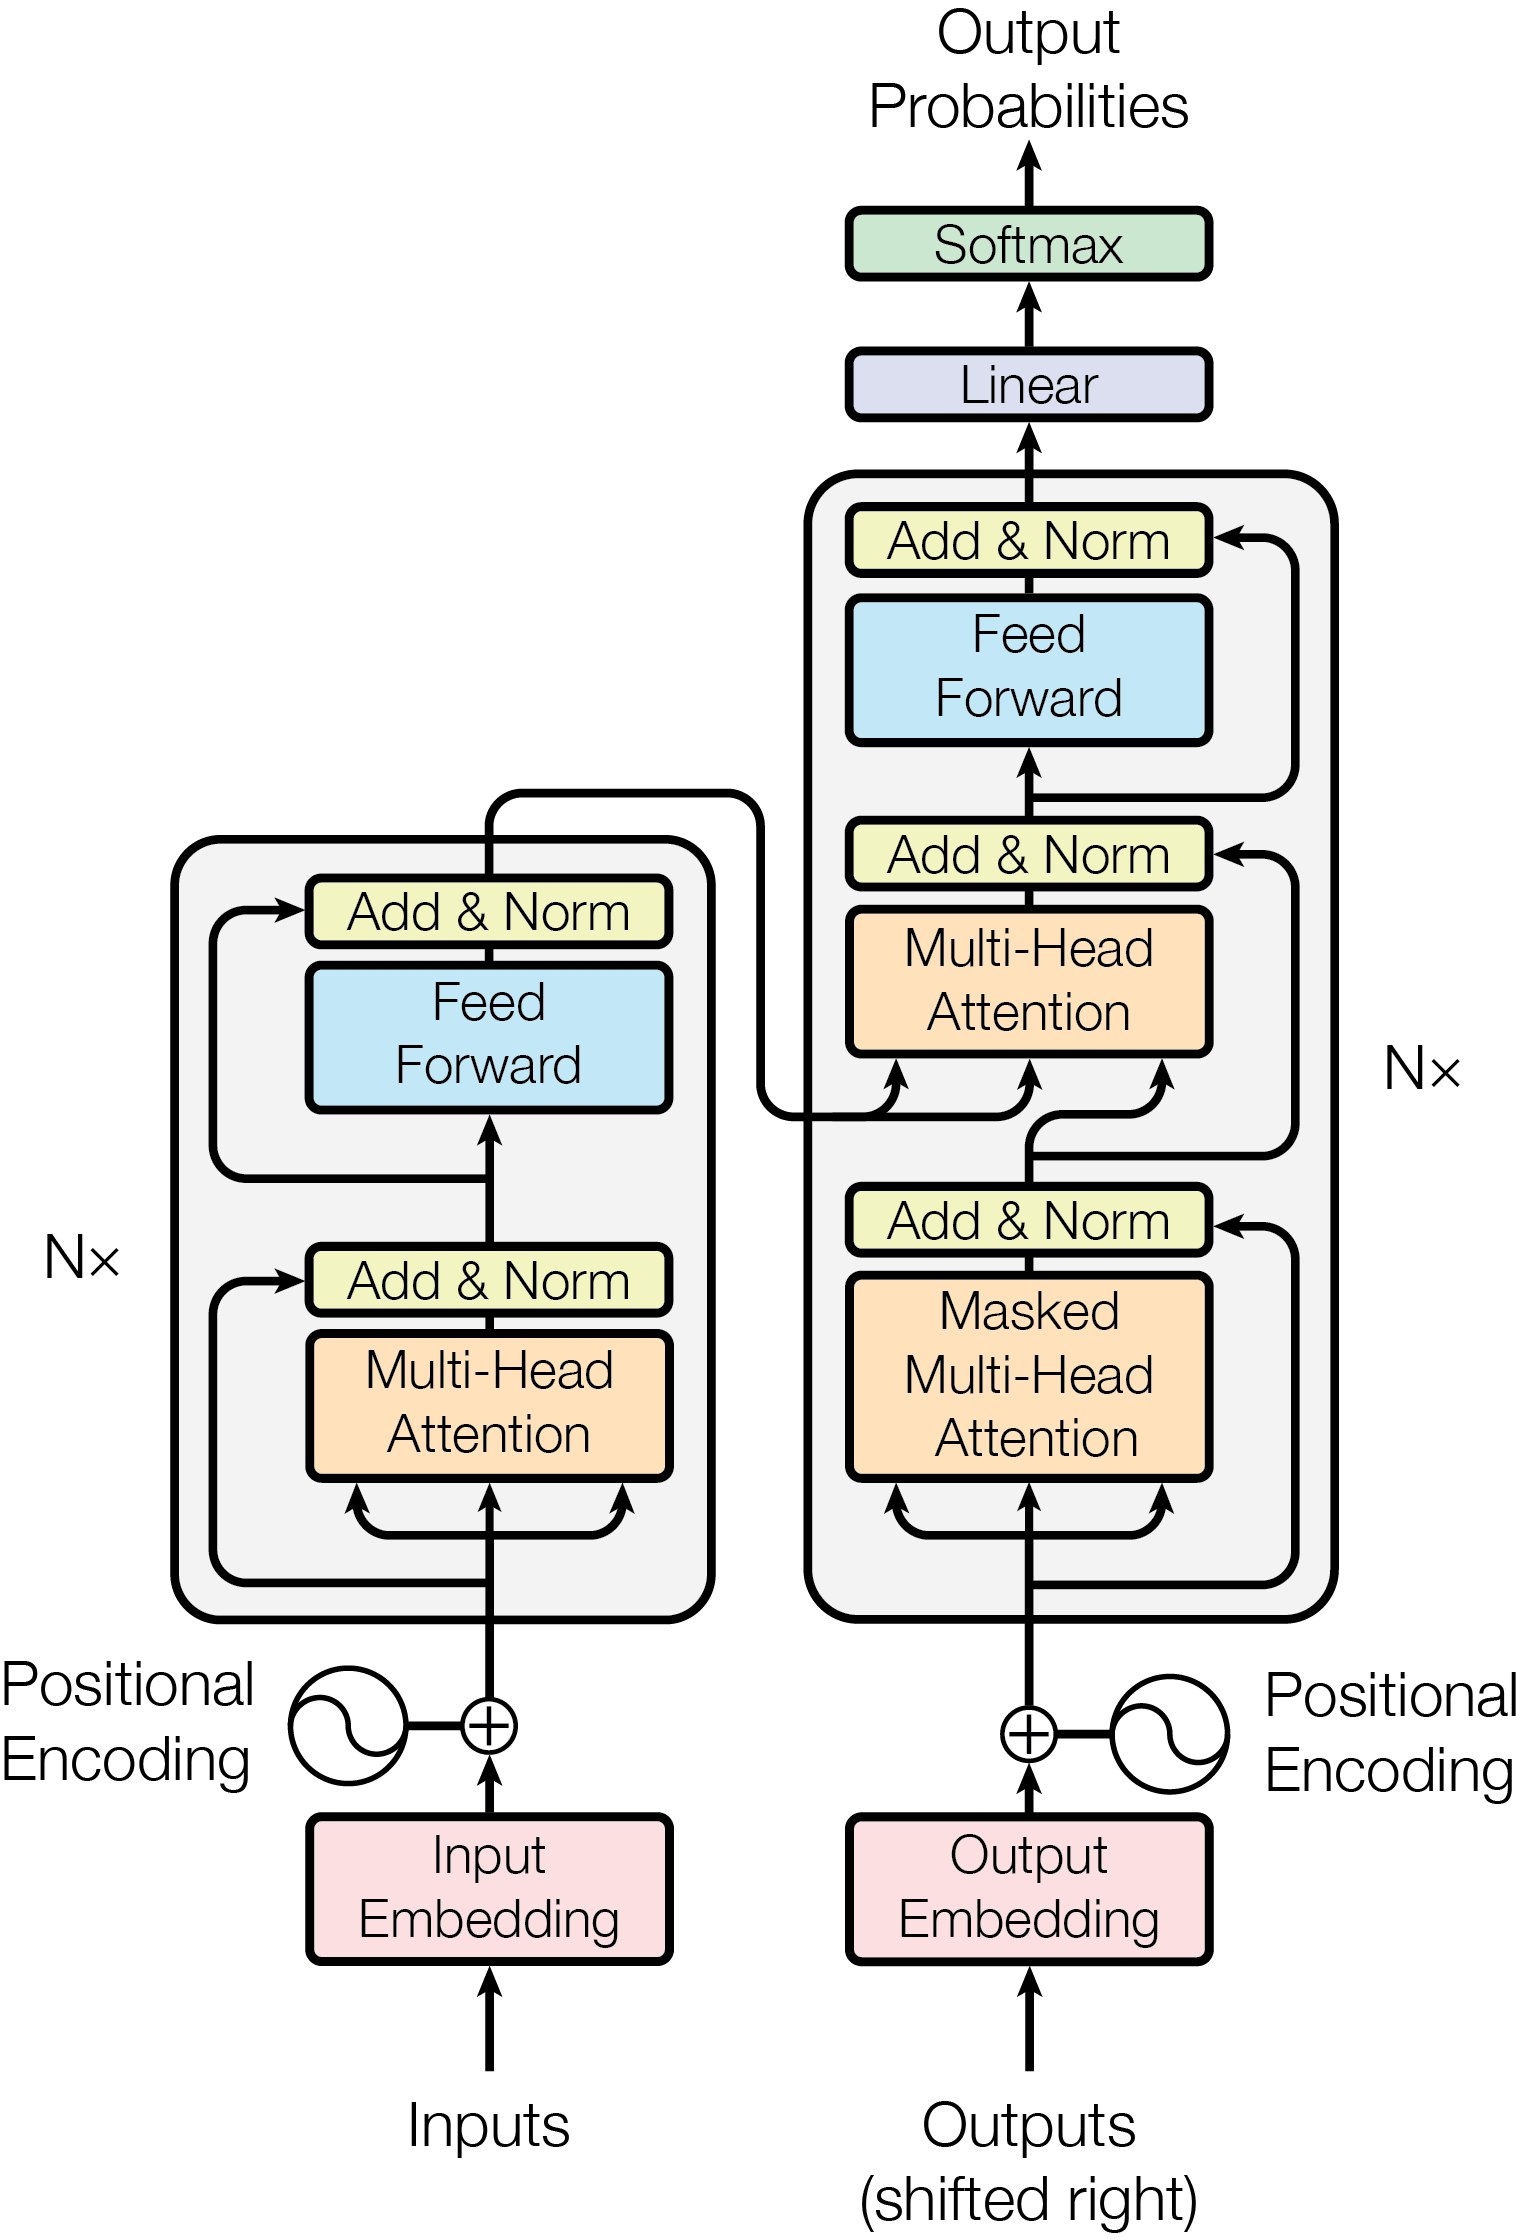
\includegraphics[width=6 cm]{3_ChapterTranformerVariants/figuras/Transformer_architecture.png}
    \caption{The Transformer - model architecture, }
    \LABFIG{FIG}
    \end{figure}

\subsubsection{Encoder-Decoder Structure}

\noindent\textbf{Encoder}

\noindent Each encoder layer in the Transformer model is composed of two primary sub-layers. The first sub-layer is the multi-head self-attention mechanism. This mechanism allows the model to focus on different parts of the input sequence simultaneously, capturing various aspects of the input data. By using multiple attention heads, the model can learn to attend to different positions in the sequence, which helps in understanding the context and relationships between different elements in a sequence more effectively.

The second sub-layer is the fully connected feed-forward network. This network is applied to each position independently and identically, consisting of two linear transformations with a ReLU activation in between. This sub-layer helps in further processing the information extracted by the self-attention mechanism, adding non-linearity and enabling the model to learn more complex patterns.

Both sub-layers are followed by layer normalization and residual connections. Layer normalization helps in stabilizing the training process by normalizing the inputs to each sub-layer, while residual connections allow the model to retain information from previous layers, facilitating better gradient flow and improving the overall training efficiency.
\vspace{10pt}

\noindent\textbf{Decoder}

\noindent The decoder in the Transformer model also consists of multiple layers, each containing three main sub-layers. The first sub-layer is the masked multi-head self-attention mechanism. Unlike the encoder's self-attention, this mechanism is masked to prevent the decoder from attending to future positions in the sequence, ensuring that the prediction for a particular position only depends on the known outputs up to that position.

The second sub-layer is the encoder-decoder attention mechanism. This mechanism allows the decoder to focus on relevant parts of the input sequence by attending to the encoder's output. It helps the decoder to incorporate information from the entire input sequence, which is crucial for generating accurate and contextually appropriate outputs.

The third sub-layer is the same fully connected feed-forward network used in the encoder. This sub-layer further processes the combined information from the self-attention and encoder-decoder attention mechanisms.

Similar to the encoder, each of these sub-layers in the decoder is followed by layer normalization and residual connections. These components ensure stable training and efficient information flow throughout the network.
\vspace{10pt}

\subsubsection{Self-Attention Mechanism}
At the core of the Transformer architecture is the self-attention mechanism, which enables the model to weigh the importance of different elements in an input sequence dynamically. The self-attention mechanism computes a set of attention scores for each element in the sequence, determining how much focus each element should have on every element in the sequence.
\vspace{10pt}

\noindent\textbf{Scaled Dot-Product Attention}

\noindent The self-attention mechanism operates through a process called scaled dot-product attention, which can be broken down into several key steps:

\begin{enumerate}
    \item \textbf{Calculate Query (Q), Key (K), and Value (V) Vectors}: For each element in the input sequence, the model generates three vectors: a query vector (Q), a key vector (K), and a value vector (V). These vectors are derived from the element embeddings using learned linear transformations.
    \item \textbf{Compute Attention Scores}: The attention score for each element pair is computed by taking the dot product of the query vector of the current element with the key vector of another element. This measures the relevance of one element to another.
    \item \textbf{Scale the Attention Scores}: To prevent the dot product values from becoming too large and destabilizing the learning process, the attention scores are scaled by dividing by the square root of the dimensionality of the key vectors ($\sqrt{d_k}$).
    \item \textbf{Apply Softmax Function}: The scaled attention scores are then passed through a softmax function to convert them into probabilities, ensuring that the scores for each element sum to 1. These probabilities are known as attention weights.
    \item \textbf{Weighted Sum of Value Vectors}: The final attention output for each element is obtained by taking a weighted sum of the value vectors, using the attention weights as coefficients.
\end{enumerate}

The entire process is summarized by the following formula:

\[
\text{Attention}(Q, K, V) = \text{softmax}\left(\frac{QK^T}{\sqrt{d_k}}\right)V
\]

\begin{figure}[htbp]
    \centering
    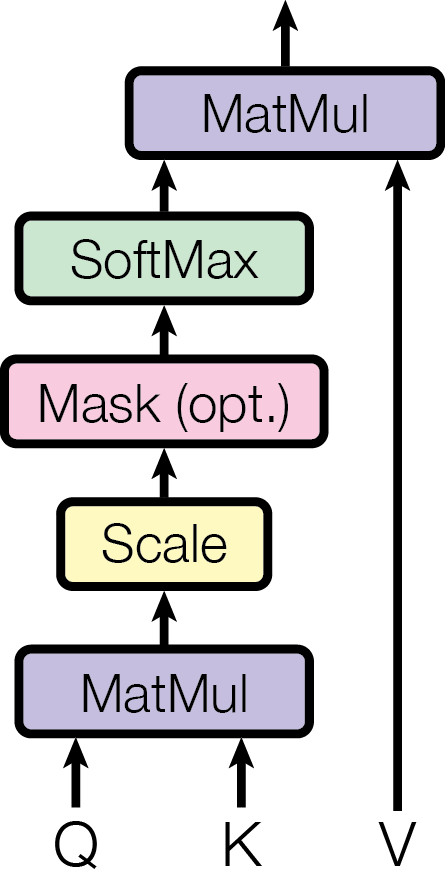
\includegraphics[width=3 cm]{3_ChapterTranformerVariants/figuras/ScaledDotProductAttention.png}
    \caption{Scaled Dot-Product Attention, from \textit{"Attention Is All You Need"} (Vaswani, et al., 2017) \cite{vaswani2023attention}}
    \LABFIG{FIG}
    \end{figure}

\noindent\textbf{Multi-Head Attention}

\noindent Instead of performing a single attention function, the Transformer employs multiple attention heads. Each head performs its own attention operation in parallel, allowing the model to capture different aspects of relationships between different elements in sequence. The outputs of all heads are then concatenated and linearly transformed to produce the final attention output.

\[
\text{MultiHead}(Q,K,V) = \text{Concat}(\text{head}_1, \ldots, \text{head}_h) W^O
\]

\noindent where each head is defined as:

\[
\text{head}_i = \text{Attention}(QW_i^Q, KW_i^K, VW_i^V)
\]

\begin{figure}[htbp]
    \centering
    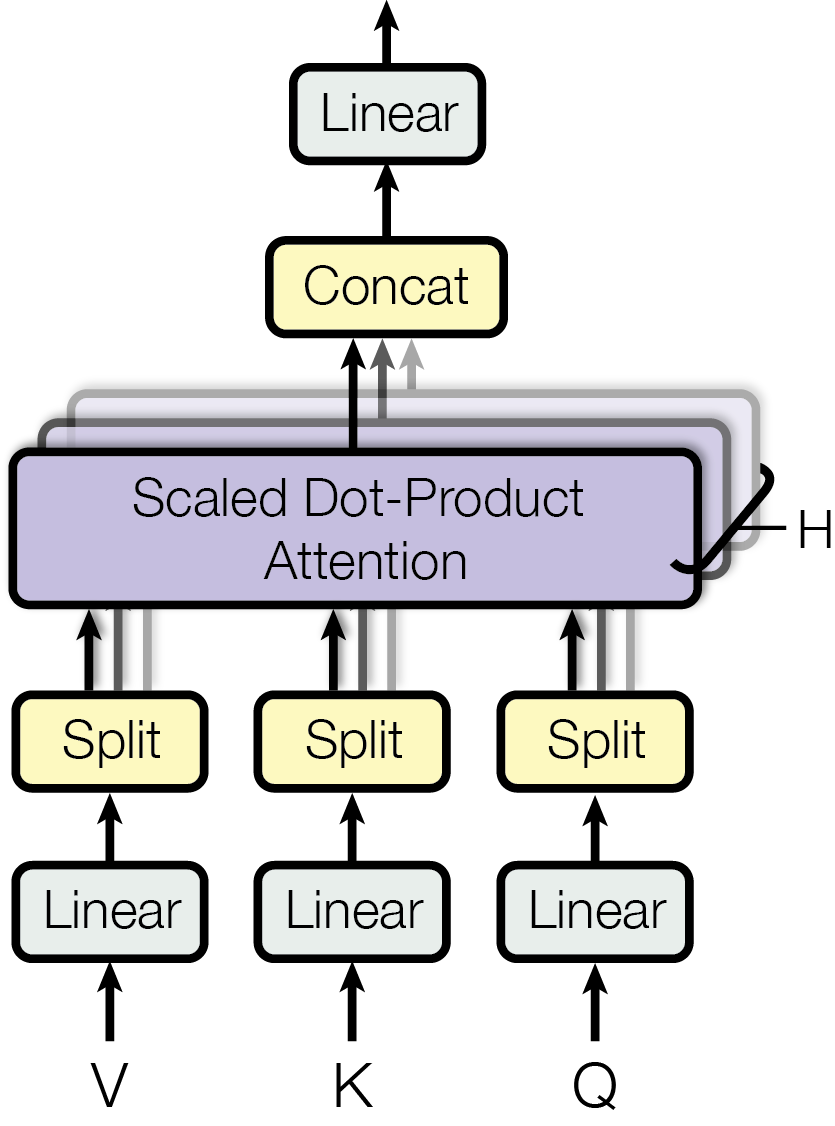
\includegraphics[width=5cm]{3_ChapterTranformerVariants/figuras/MultiHeadAttention.png}
    \caption{Multi-Head Attention, from \textit{"Attention Is All You Need"} (Vaswani, et al., 2017) \cite{vaswani2023attention}}
    \LABFIG{FIG}
    \end{figure}

%%%%%%%%%%%%%%%%%%%%%%%%%%%%%%%%%%%%%%%%%%%%%%%%%%%%%%%%%%%%%%%%
\section{Time Series Transformer}

Previously, we explored the Transformer architecture. Now, we turn our focus to the Time Series Transformer, designed specifically for time series forecasting. As well as the original Transformer, this model is built around two main components: the Encoder and the Decoder. The Encoder processes past time series values, capturing essential patterns and dependencies. Meanwhile, the Decoder uses this encoded information to predict future values, integrating temporal features to enhance prediction accuracy.

Time series forecasting involves predicting future values based on historical data. The Time Series Transformer tackles this through embeddings, which convert categorical data into continuous vectors, capturing temporal dependencies effectively. These embeddings include channel projection and timestamp embeddings, which help the model understand both local and global temporal dynamics.

Training the model involves a method called teacher-forcing, where the model learns correct sequence patterns by using actual previous values during training. Additionally, the Time Series Transformer employs probabilistic forecasting to quantify uncertainty in predictions, which is crucial for real-world decision-making.

\subsection{Time Series Forecasting (TSF) Problem Formulation}
Time series forecasting (TSF) involves predicting future values based on previously observed data. For a time series containing \(C\) variates, the historical data can be represented as:
\[
X = \{X^t_1, \ldots, X^t_C\}_{t=1}^L
\]
where \(L\) is the look-back window size and \(X^t_i\) is the value of the \(i\)-th variate at the \(t\)-th time step. The goal of TSF is to predict the future values:
\[
\hat{X} = \{\hat{X}^t_1, \ldots, \hat{X}^t_C\}_{t=L+1}^{L+T}
\]
for the next \(T\) time steps.

When \(T > 1\), there are two main approaches to multi-step forecasting:
\begin{itemize}
    \item \textbf{Iterated Multi-Step (IMS) Forecasting:} This approach learns a single-step forecaster and iteratively applies it to obtain multi-step predictions. While IMS predictions tend to have smaller variance due to the autoregressive estimation procedure, they are prone to error accumulation effects. Therefore, IMS forecasting is preferable when there is a highly accurate single-step forecaster and \(T\) is relatively small.
    \begin{figure}[htbp]
        \centering
        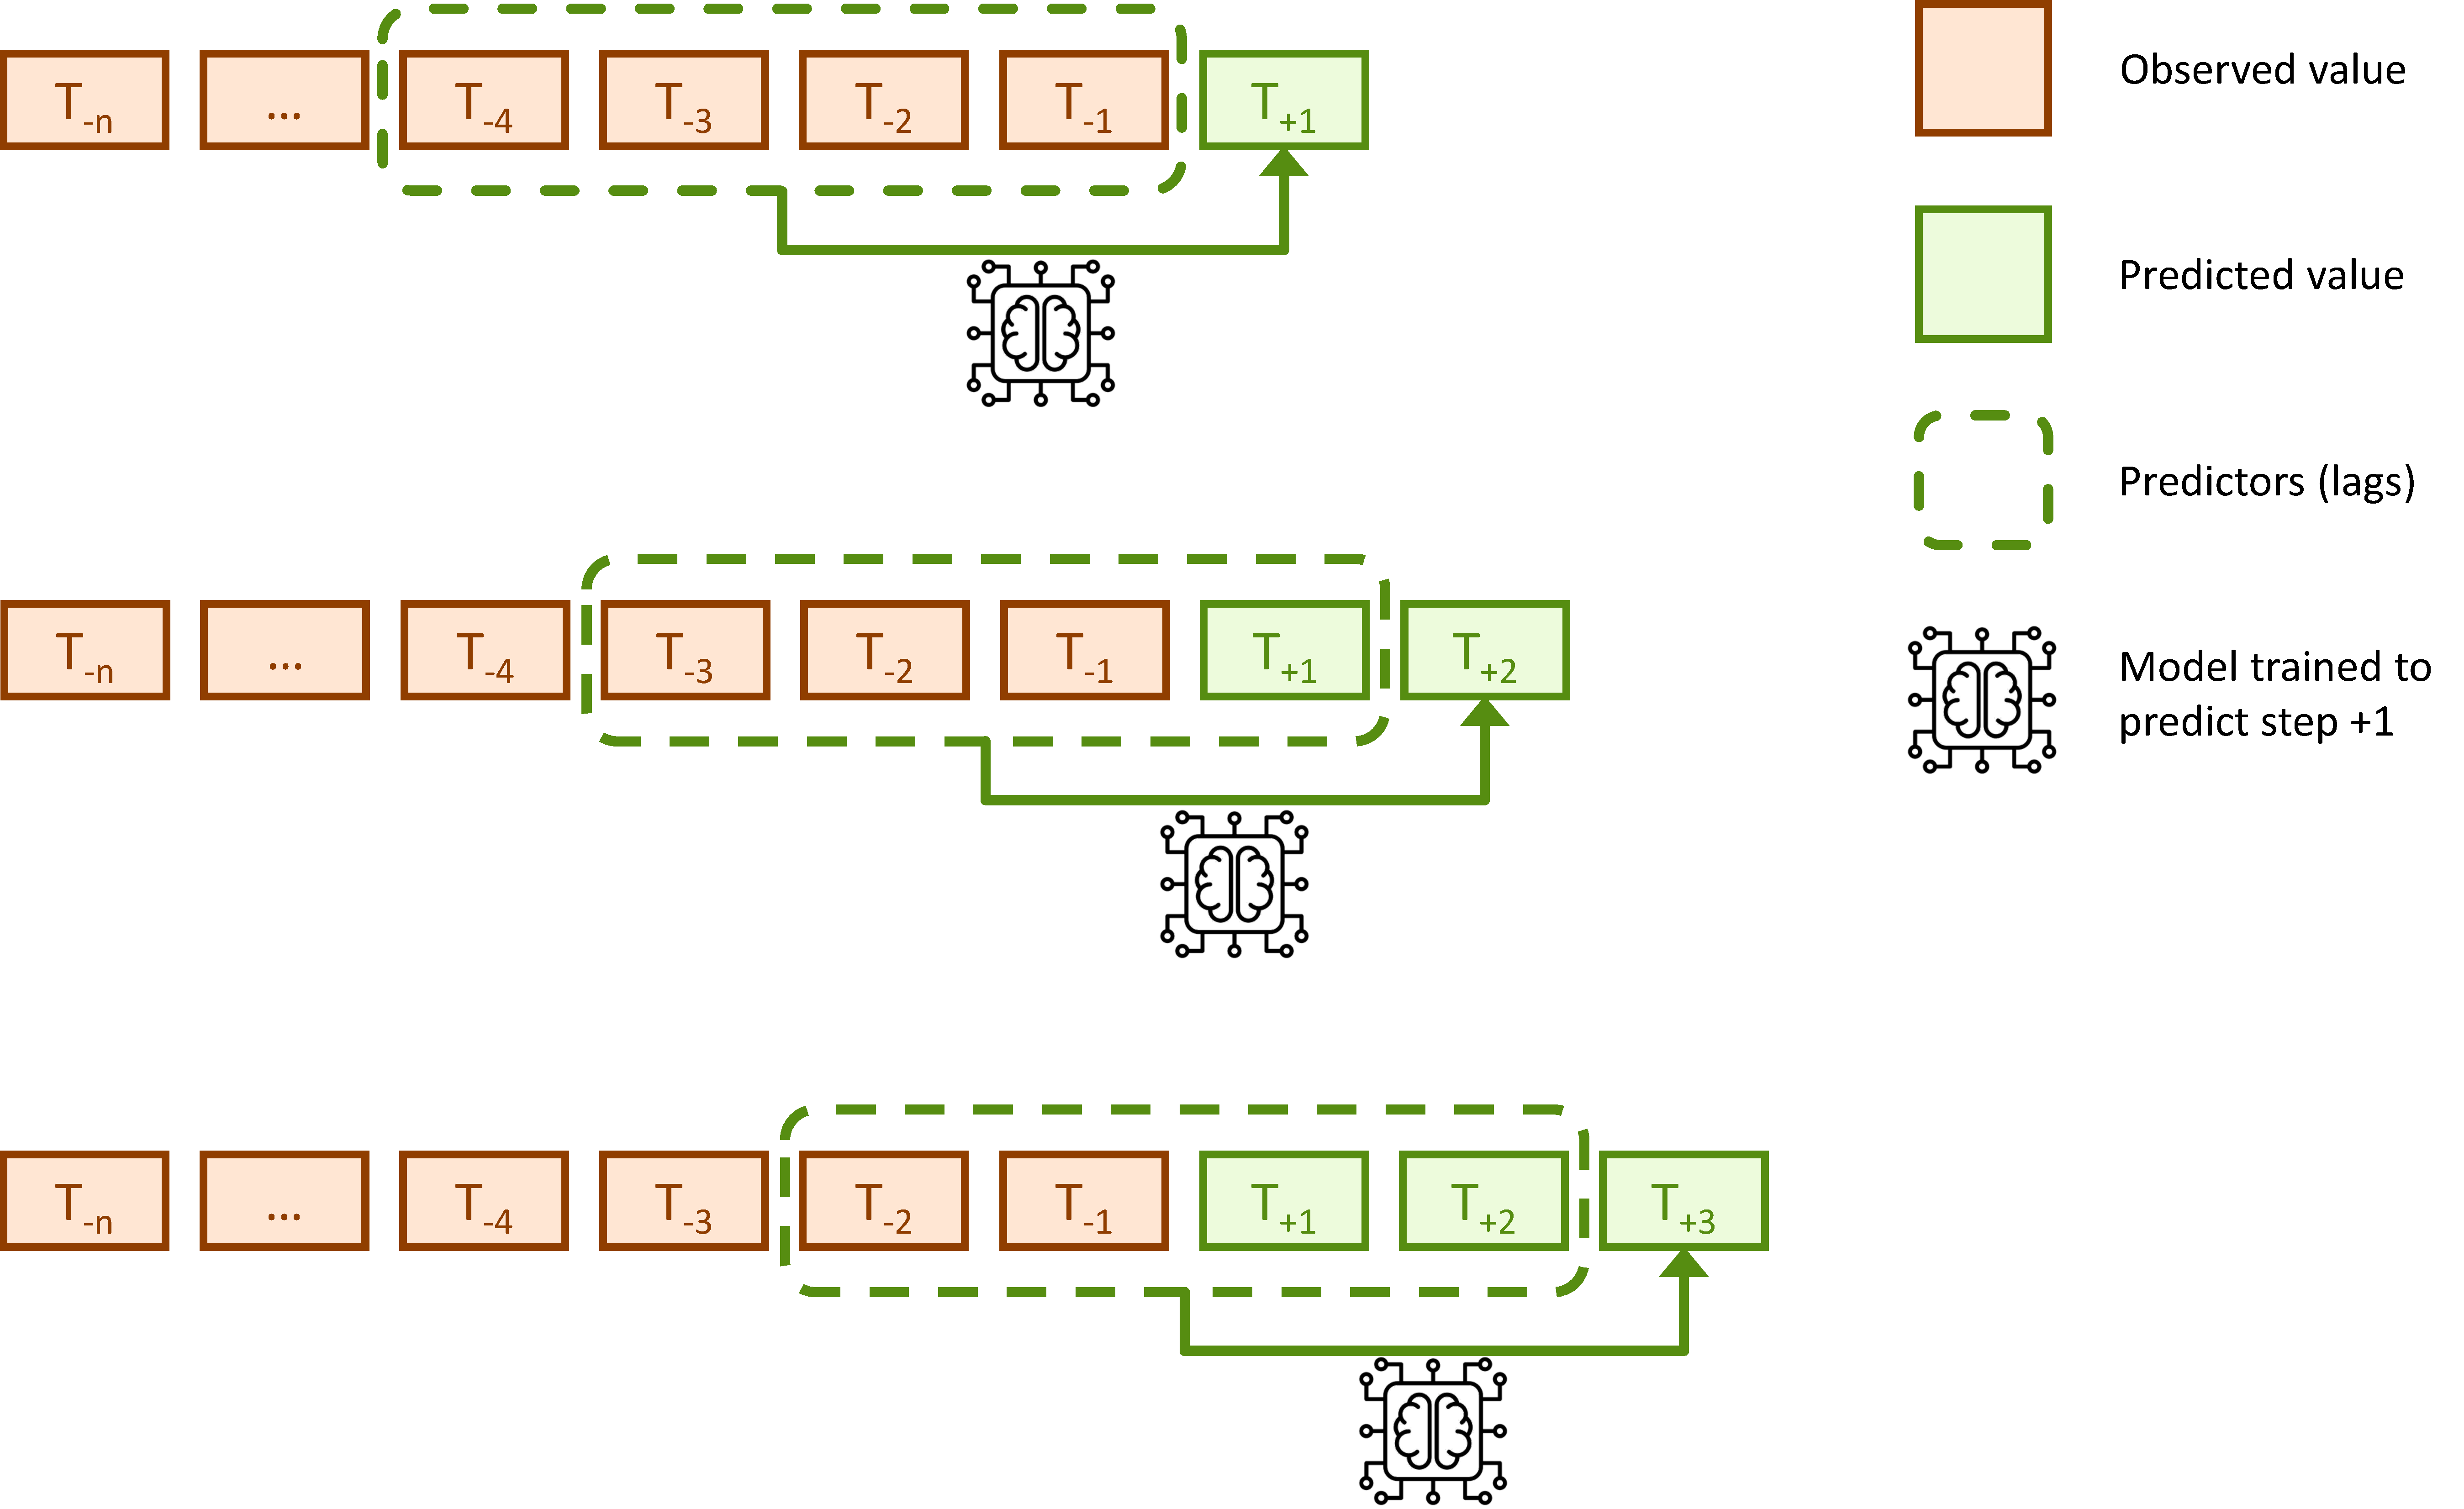
\includegraphics[width=13cm]{3_ChapterTranformerVariants/figuras/IMS.pdf}
        \caption{Illustration of Iterated Multi-Step (IMS) Forecasting}
        \LABFIG{FIG}
        \end{figure}
    
    \item \textbf{Direct Multi-Step (DMS) Forecasting:} This approach directly optimizes the multi-step forecasting objective at once. DMS forecasting generates more accurate predictions when it is challenging to obtain an unbiased single-step forecasting model or when \(T\) is large.
    \begin{figure}[htbp]
        \centering
        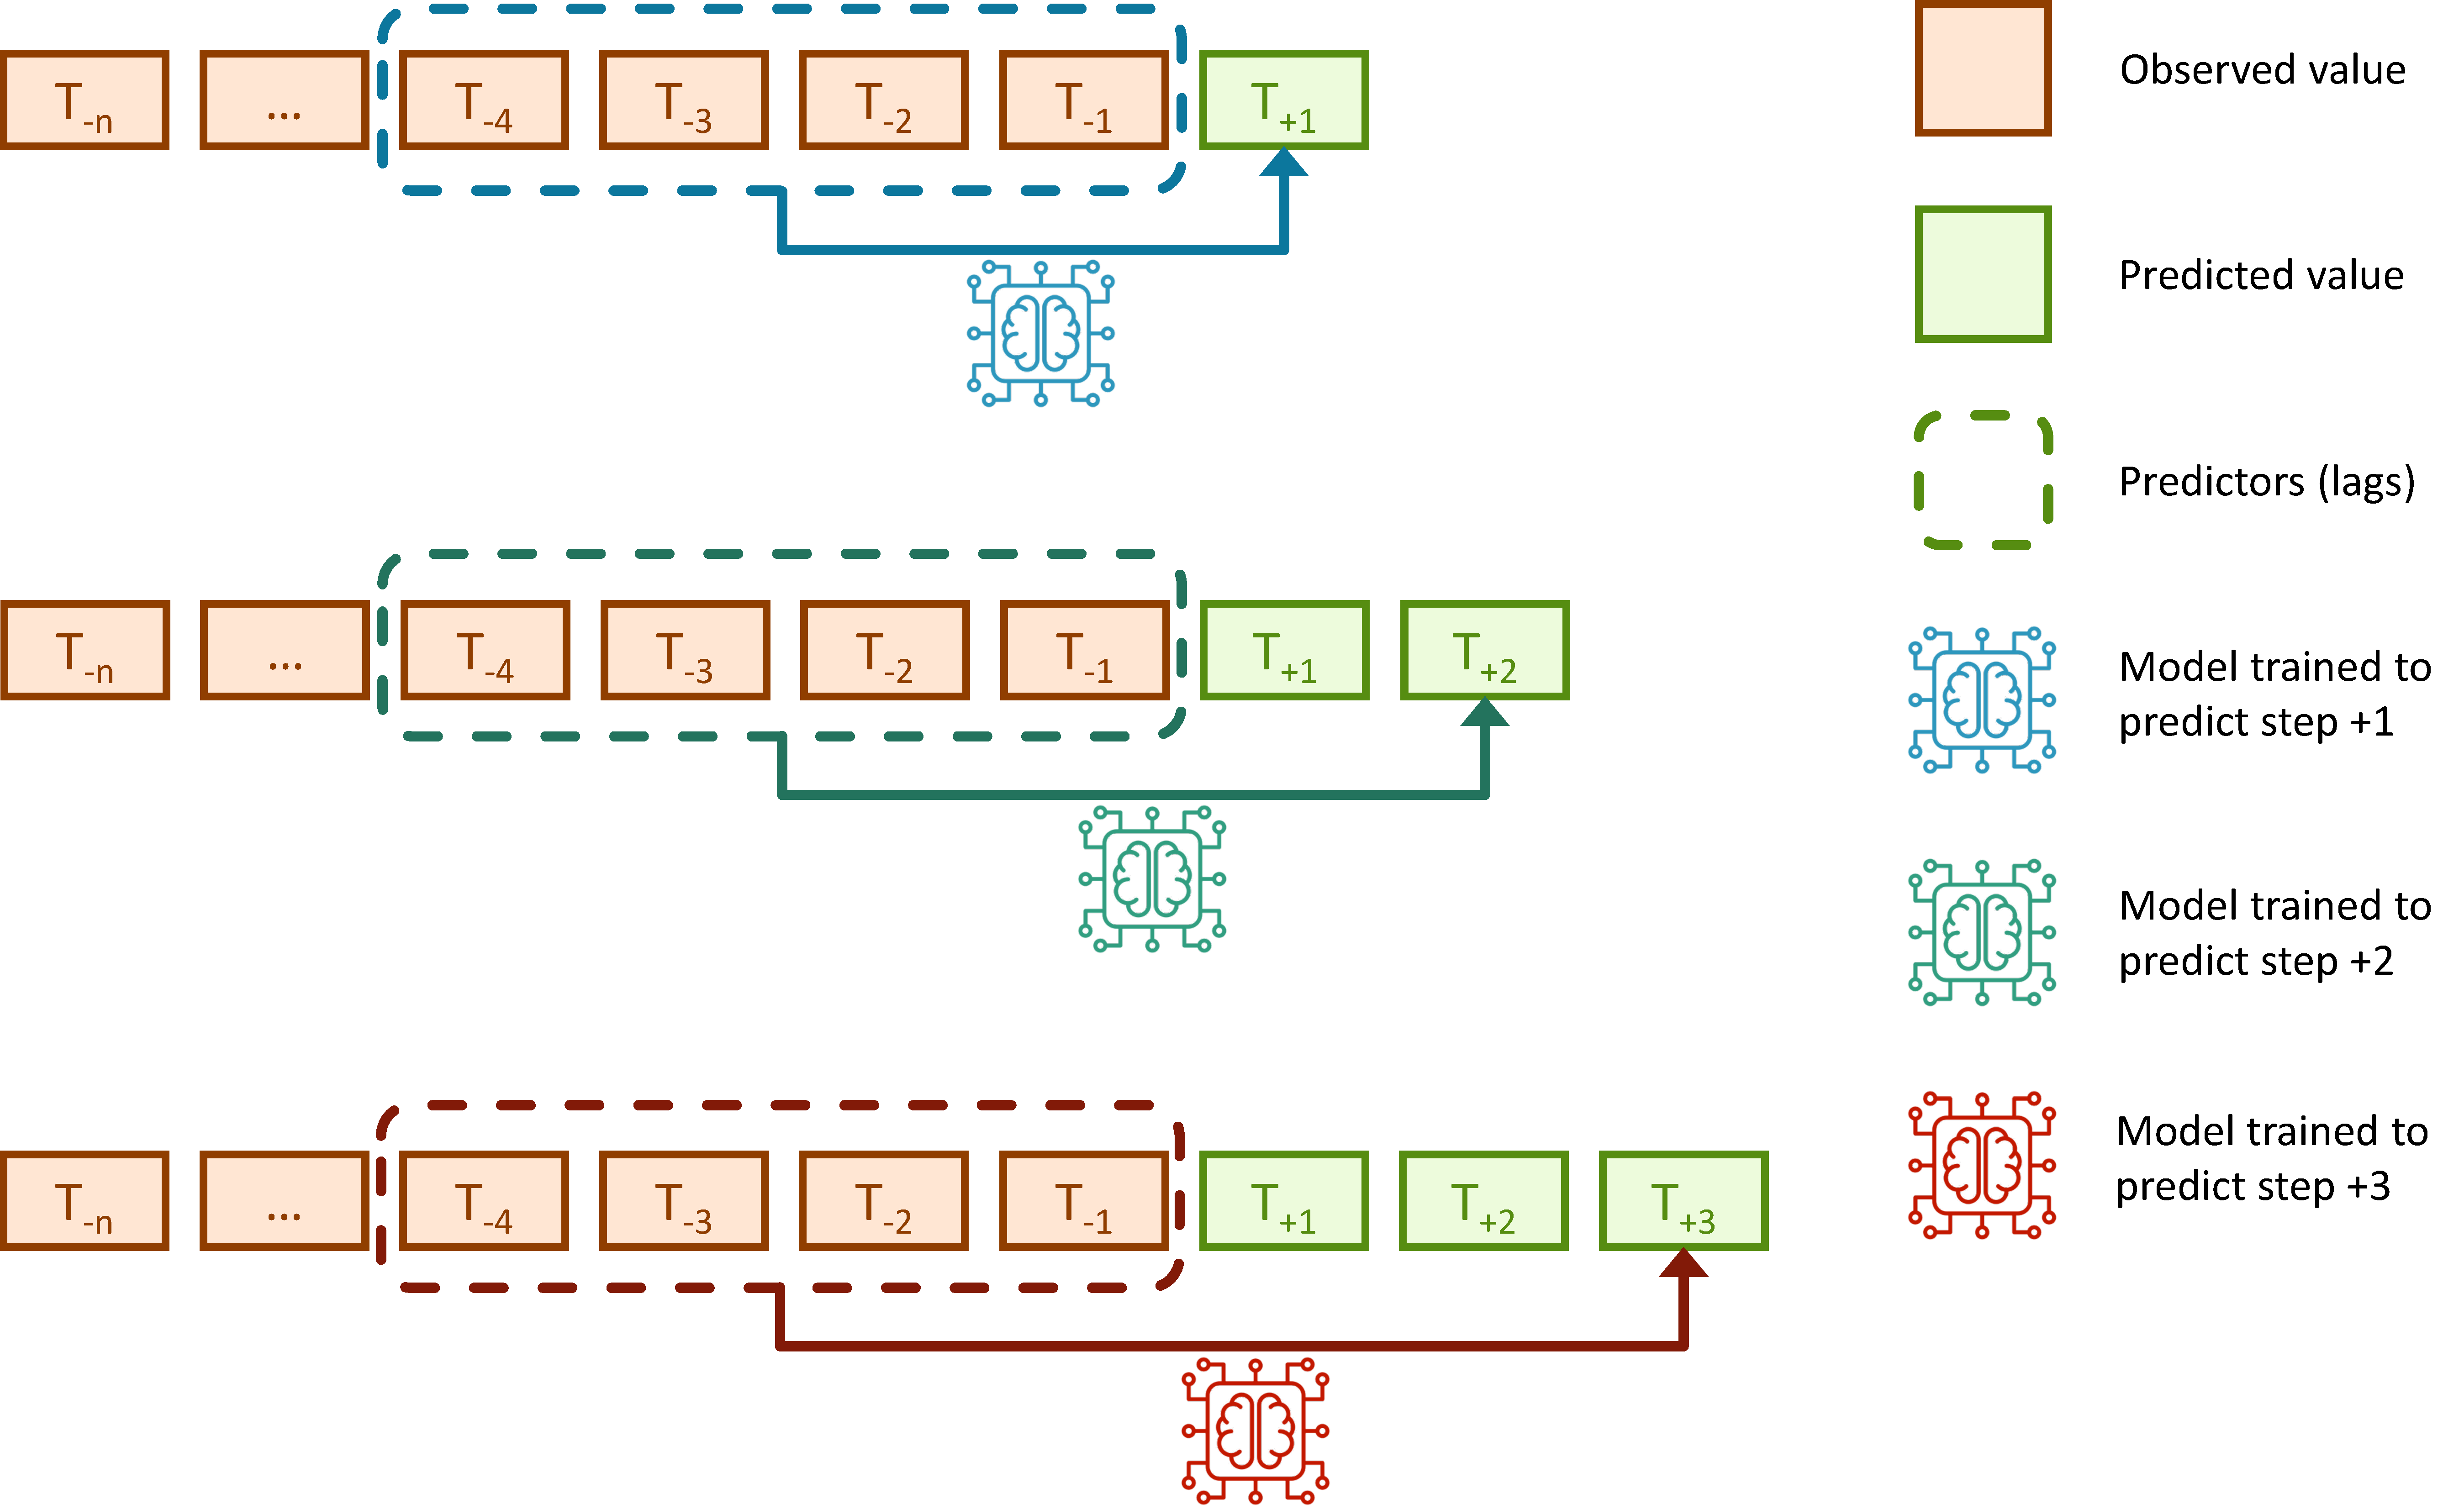
\includegraphics[width=13cm]{3_ChapterTranformerVariants/figuras/DMS.pdf}
        \caption{Illustration of Direct Multi-Step (DMS) Forecasting}
        \LABFIG{FIG}
        \end{figure}
    
\end{itemize}

\subsection{Embedding}
Embeddings are a crucial component in the field of machine learning and natural language processing. They are used to convert categorical data into continuous vector representations, which can then be fed into machine learning models. In the context of time series forecasting, embeddings help in capturing the temporal dependencies and patterns within the data, enabling the model to make accurate predictions.

To adapt the Transformer architecture for time series forecasting, the embedding process involves several key components: channel projection, fixed position, local timestamp, and global timestamp. Each of these components plays a vital role in ensuring that the model effectively captures the temporal dynamics of the data.

\subsubsection{Channel Projection}
Channel projection is the process of transforming the input time series data into a higher-dimensional space. This is done to capture the complex relationships between different channels (or features) of the time series data. By projecting the data into a higher-dimensional space, the model can better understand the interactions between different channels and make more accurate predictions.
\begin{figure}[htbp]
    \centering
    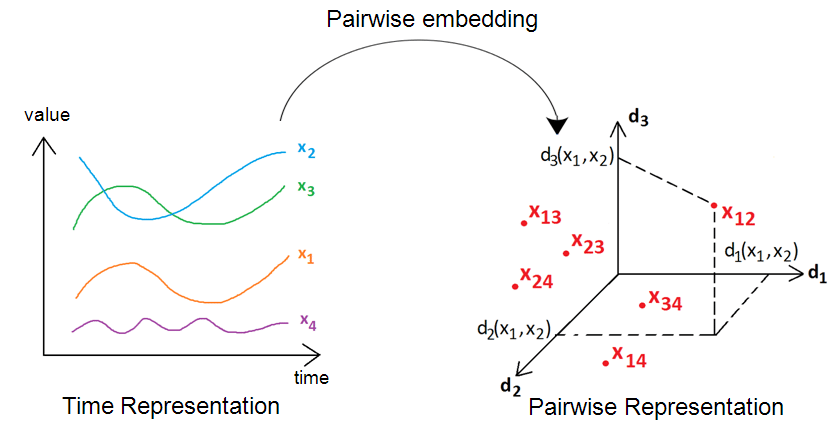
\includegraphics[width=13cm]{3_ChapterTranformerVariants/figuras/ChannelProjection.png}
    \caption{Example of embedding of time series xi from the temporal space (left) into the pairwise space (right). In this example, a pair of time series (x1, x2) is projected into the pairwise space as a vector x12 described by p = 3 basic metrics: x12 = [d1(x1, x2), d2(x1, x2), d3(x1, x2)] T, from \textit{"Multiple Metric Learning for large margin kNN Classification of time series"} \cite{inproceedings}}
    \LABFIG{FIG}
    \end{figure}

\subsubsection{Fixed Position Embedding}
As we explained before, fixed position embedding is used to encode the positional information of the time series data. In the Transformer architecture, positional encodings are added to the input embeddings to provide the model with information about the order of the data points. This is crucial for time series forecasting, as the temporal order of the data points is essential for making accurate predictions. Fixed position embeddings are typically generated using sinusoidal functions, which provide a unique encoding for each position in the sequence.

\subsubsection{Local Timestamp Embedding}
Local timestamp embedding captures the local temporal information within the time series data. This includes information such as the time of day, day of the week, or any other relevant local temporal features. By incorporating local timestamp embeddings, the model can better understand the short-term patterns and trends within the data, leading to more accurate forecasts.

For example, consider a data point recorded at 3 PM on a Wednesday. The local timestamp embedding would capture the hour of the day (15), the day of the week (3 for Wednesday), and the day of the month (15).

\subsubsection{Global Timestamp Embedding}
Global timestamp embedding captures the global temporal information across the entire time series. This includes long-term trends and seasonal patterns that may not be immediately apparent from the local temporal information. By incorporating global timestamp embeddings, the model can better understand the overall temporal dynamics of the data, leading to more accurate long-term forecasts.

For example, imagine a data point recorded in July 2024. The global timestamp embedding would include the month of the year (7 for July), the quarter of the year (3 for July to September), and the year (2024).

\begin{figure}[htbp]
    \centering
    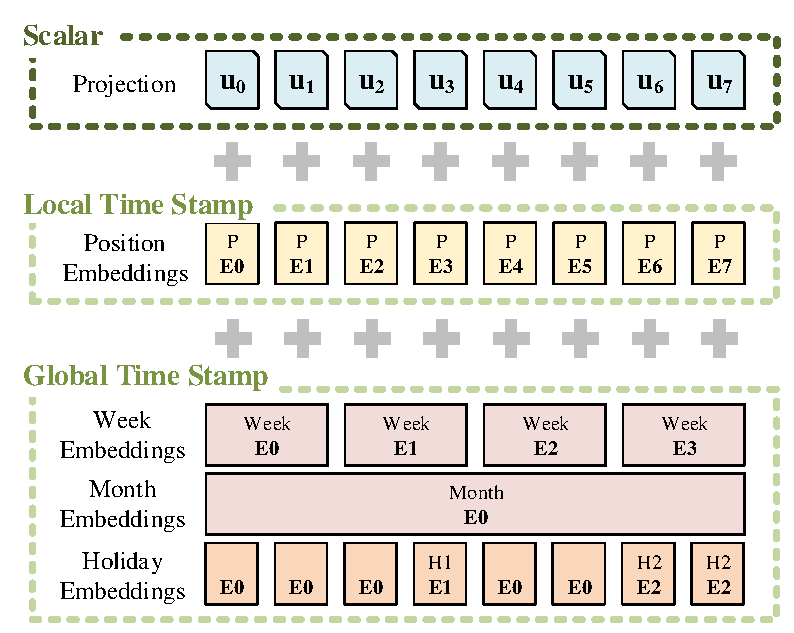
\includegraphics[width=10cm]{3_ChapterTranformerVariants/figuras/Embbeding.pdf}
    \caption{The input representation of a Time Series Transformer, from Informer (Zhou, et al., 2019)\cite{zhou2021informerefficienttransformerlong}}
    \LABFIG{FIG}
    \end{figure}



\subsection{Encoder}
The Encoder’s role is to process a sequence of past time series values, known as \textit{past\_values}. It effectively captures the temporal patterns and dependencies within these values. In addition to the raw \textit{past\_values}, the Encoder takes the data from the embedding, which includes local timestamps and other relevant temporal features, to provide the model with more temporal context.

\subsection{Decoder}
The Decoder’s role is to predict future time series values, known as \textit{future\_values}, based on the encoded information from \textit{past\_values}. The Decoder generates a sequence of predictions for the desired forecast horizon. Like the Encoder, the Decoder can incorporate future time features to provide temporal context for the predictions. These features are analogous to the past time features.

\subsection{Training Methodology}
Training a Time Series Transformer involves a process called \textit{teacher-forcing}. This method is crucial for effectively training sequence-to-sequence models, such as those used in time series forecasting.

Teacher-forcing is a technique where the model is trained to predict the next value in a sequence by using the actual previous value rather than the model's own previous prediction. This helps the model learn the correct sequence patterns more efficiently and reduces the accumulation of errors during training.

Here's a step-by-step breakdown of how we train the Time Series Transformer:
\begin{enumerate}
    \item \textbf{Preparing the Training Data:}
    \begin{itemize}
        \item We start with pairs of \textit{past\_values} and \textit{future\_values}.
        \item \textit{past\_values} represent the known historical data up to the current time step.
        \item \textit{future\_values} represent the target values we aim to predict.
    \end{itemize}
    \item \textbf{Shifting Future Values:}
    \begin{itemize}
        \item The \textit{future\_values} sequence is shifted one position to the right.
        \item This creates a new sequence where each time step corresponds to the next time step in the original \textit{future\_values}.
    \end{itemize}
    \item \textbf{Initial Input for the Decoder:}
    \begin{itemize}
        \item The last value of \textit{past\_values} is used as the initial input for the Decoder.
        \item This value acts as the starting point for generating the first prediction in the \textit{future\_values} sequence.
    \end{itemize}
    \item \textbf{Training with Teacher-Forcing:}
    \begin{itemize}
        \item During training, the model uses the actual previous value from the \textit{future\_values} sequence as the input for the next time step.
        \item This ensures that the model is conditioned on the correct context at each step, helping it learn the dependencies more accurately.
    \end{itemize}
    \item \textbf{Loss Calculation and Backpropagation:}
    \begin{itemize}
        \item The model's predictions are compared to the actual \textit{future\_values} to calculate the loss.
        \item The loss is then backpropagated through the model to update the weights and improve the predictions.
    \end{itemize}
\end{enumerate}

The use of teacher-forcing in training Time Series Transformers is essential for achieving accurate and stable predictions. By providing the model with the correct context at each step, we ensure that it learns the correct sequence patterns and dependencies, leading to better performance in time series forecasting tasks.


\subsection{Probabilistic Forecasting}
Unlike classical point forecasting methods that output a single value per time step, the Time Series Transformer is designed for probabilistic forecasting. This approach models a distribution from which predictions can be sampled, providing a measure of uncertainty in the forecasts. This is particularly useful in real-world decision-making processes where understanding the range of possible outcomes is crucial.

Deep learning models, including Transformers, excel in this context by learning from multiple related time series and modeling data uncertainty effectively. Probabilistic forecasting can be implemented by learning future parameters of a parametric distribution or using techniques like conformal prediction adapted for time series.

According to the paper \textit{"Use and Communication of Probabilistic Forecasts"} (Adrian E. Raftery)\cite{raftery2014usecommunicationprobabilisticforecasts}, probabilistic forecasts are becoming increasingly available and are essential for various types of users, including general assessors, change assessors, risk avoiders, and decision theorists. These forecasts provide valuable insights by quantifying the uncertainty and offering a range of possible outcomes, which can be summarized using probabilities of adverse events and percentiles of the predictive distribution. Effective communication of probabilistic forecasts involves interacting with users to understand their goals and minimizing cognitive load by presenting the information in a clear and concise manner. This ensures that the forecasts are not only accurate but also trusted and actionable in practical applications.

\begin{figure}[htbp]
    \centering
    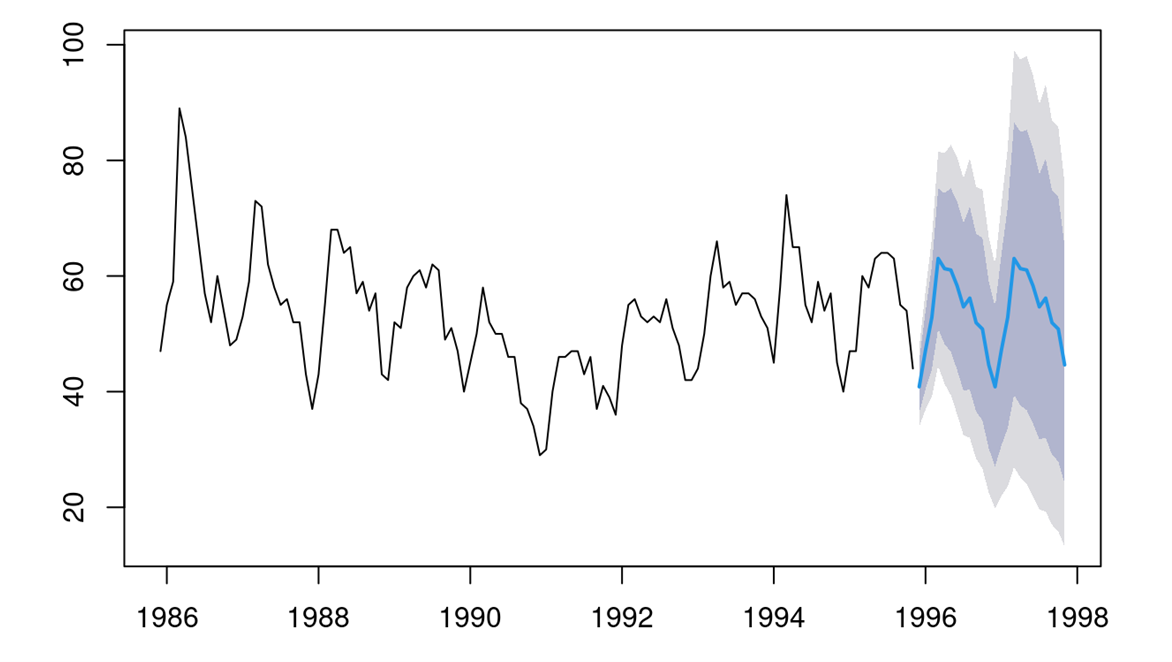
\includegraphics[width=10cm]{3_ChapterTranformerVariants/figuras/Probabilistic.png}
    \caption{Ilustration of Probabilistic Forecasting}
    \LABFIG{FIG}
    \end{figure}





%%%%%%%%%%%%%%%%%%%%%%%%%%%%%%%%%%%%%%%%%%%%%%%%%%%%%%%%%%%%%%%%
\section{Informer}
In December 2020, Haoyi Zhou, Shanghang Zhang, Jieqi Peng, Shuai Zhang, Jianxin Li, Hui Xiong, and Wancai Zhang introduced a groundbreaking paper titled \textit{``Informer: Beyond Efficient Transformer for Long Sequence Time-Series Forecasting''}. This paper received the prestigious AAAI-21 Best Paper Award, recognizing its significant contributions to the field.

Next, we will delve into the core components of the Informer model. We will explore the ProbSparse Attention mechanism, which enhances efficiency and performance, and the Self-Attention Distilling technique, which optimizes the handling of long sequences. By understanding these innovations, we can appreciate how the Informer model significantly advances the capabilities of time-series forecasting.

\subsection{ProbSparse Attention}
The core concept of ProbSparse attention is based on the observation that canonical self-attention scores follow a long-tail distribution. In this distribution, ``active'' queries are located in the ``head'' scores, while ``lazy'' queries are found in the ``tail'' area. An ``active'' query, denoted as \( q_i \), is one where the dot-product \( \langle q_i, k_i \rangle \) significantly contributes to the attention mechanism. Conversely, a ``lazy'' query generates a dot-product that results in trivial attention. Here, \( q_i \) and \( k_i \) represent the \( i \)-th rows in the \( Q \) and \( K \) attention matrices, respectively.

Given the distinction between ``active'' and ``lazy'' queries, ProbSparse attention focuses on selecting the ``active'' queries to form a reduced query matrix \( Q_{\text{reduced}} \). This matrix is then used to compute the attention weights with a computational complexity of \( O(T \log T) \).

\begin{figure}[htbp]
    \centering
    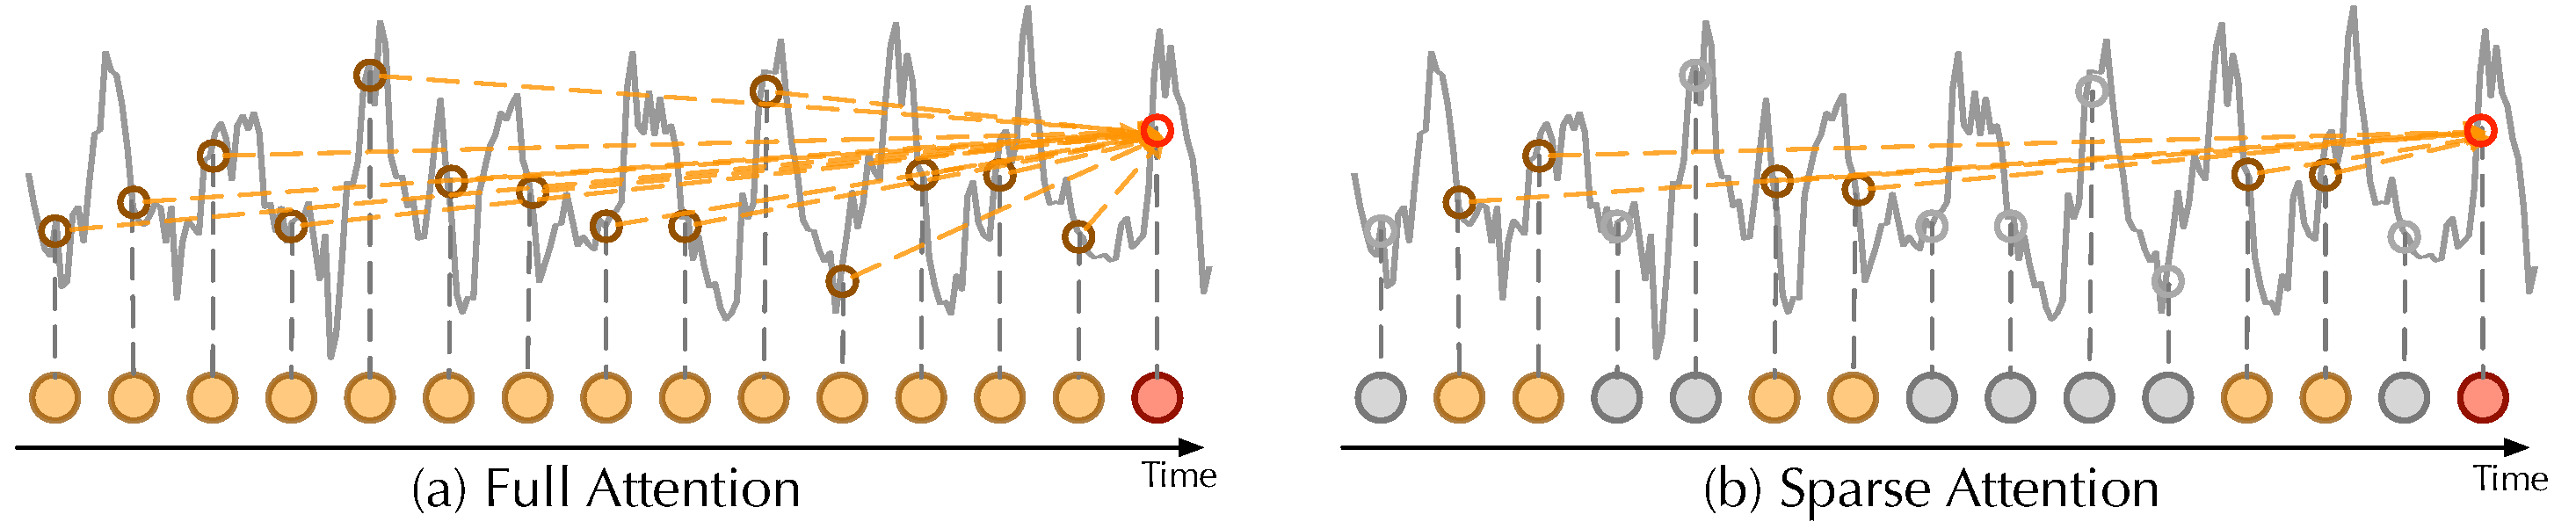
\includegraphics[width=15cm]{3_ChapterTranformerVariants/figuras/ProbSparceAttention.pdf}
    \caption{Vanilla self attention vs ProbSparse attention, from Autoformer (Wu, Haixu, et al., 2021)\cite{wu2022autoformerdecompositiontransformersautocorrelation}}
    \LABFIG{FIG}
    \end{figure}

To illustrate this, let’s revisit the canonical self-attention formula:

\[
\text{Attention}(Q, K, V) = \text{softmax}\left(\frac{QK^T}{\sqrt{d_k}}\right)V
\]

where \( Q \in \mathbb{R}^{L_Q \times d} \), \( K \in \mathbb{R}^{L_K \times d} \), and \( V \in \mathbb{R}^{L_V \times d} \). In practice, the input lengths of queries and keys are typically equivalent in self-attention computation, i.e., \( L_Q = L_K = T \), where \( T \) is the time series length. Consequently, the \( QK^T \) multiplication has a computational complexity of \( O(T^2 \cdot d) \).

In ProbSparse attention, the goal is to create a new \( Q_{\text{reduced}} \) matrix and define:

\begin{equation}
\text{ProbSparseAttention}(Q, K, V) = \text{softmax}\left(\frac{Q_{\text{reduced}} K^T}{\sqrt{d_k}}\right)V
\end{equation}

The \( Q_{\text{reduced}} \) matrix selects only the top \( u \) ``active'' queries, where \( u = c \cdot \log L_Q \) and \( c \) is the sampling factor hyperparameter for ProbSparse attention. Since \( Q_{\text{reduced}} \) selects only the top \( u \) queries, its size is \( c \cdot \log L_Q \times d \). Therefore, the multiplication \( Q_{\text{reduced}} K^T \) has a computational complexity of \( O(L_K \log L_Q) = O(T \log T) \).

The next step is to determine how to select the top \( u \) ``active'' queries to form \( Q_{\text{reduced}} \). This involves defining the Query Sparsity Measurement.
\vspace{10pt}

\noindent\textbf{Query Sparsity Measurement}

\vspace{10pt}
\noindent The Query Sparsity Measurement \( M(q_i, K) \) is used to identify the \( u \) ``active'' queries \( q_i \) within \( Q \) to construct \( Q_{\text{reduced}} \). The fundamental idea is that the dominant \( \langle q_i, k_i \rangle \) pairs cause the ``active'' \( q_i \)'s probability distribution to deviate from a uniform distribution. This deviation can be quantified using the KL divergence between the actual query distribution and the uniform distribution.

In practical terms, the measurement is defined as:

\[
M(q_i, K) = \max_j \left( \frac{q_i k_j^T}{\sqrt{d}} \right) - \frac{1}{L_k} \sum_{j=1}^{L_k} \left( \frac{q_i k_j^T}{\sqrt{d}} \right)
\]

The key insight here is that a larger \( M(q_i, K) \) value indicates that the query \( q_i \) should be included in \( Q_{\text{reduced}} \), while a smaller value suggests otherwise.

To efficiently compute this measurement, it is important to note that most dot-products \( \langle q_i, k_i \rangle \) generate trivial attention due to the long-tail distribution property. Therefore, it is sufficient to consider a representative subset of keys from \( K \) rather than the entire set.

\begin{figure}[htbp]
    \centering
    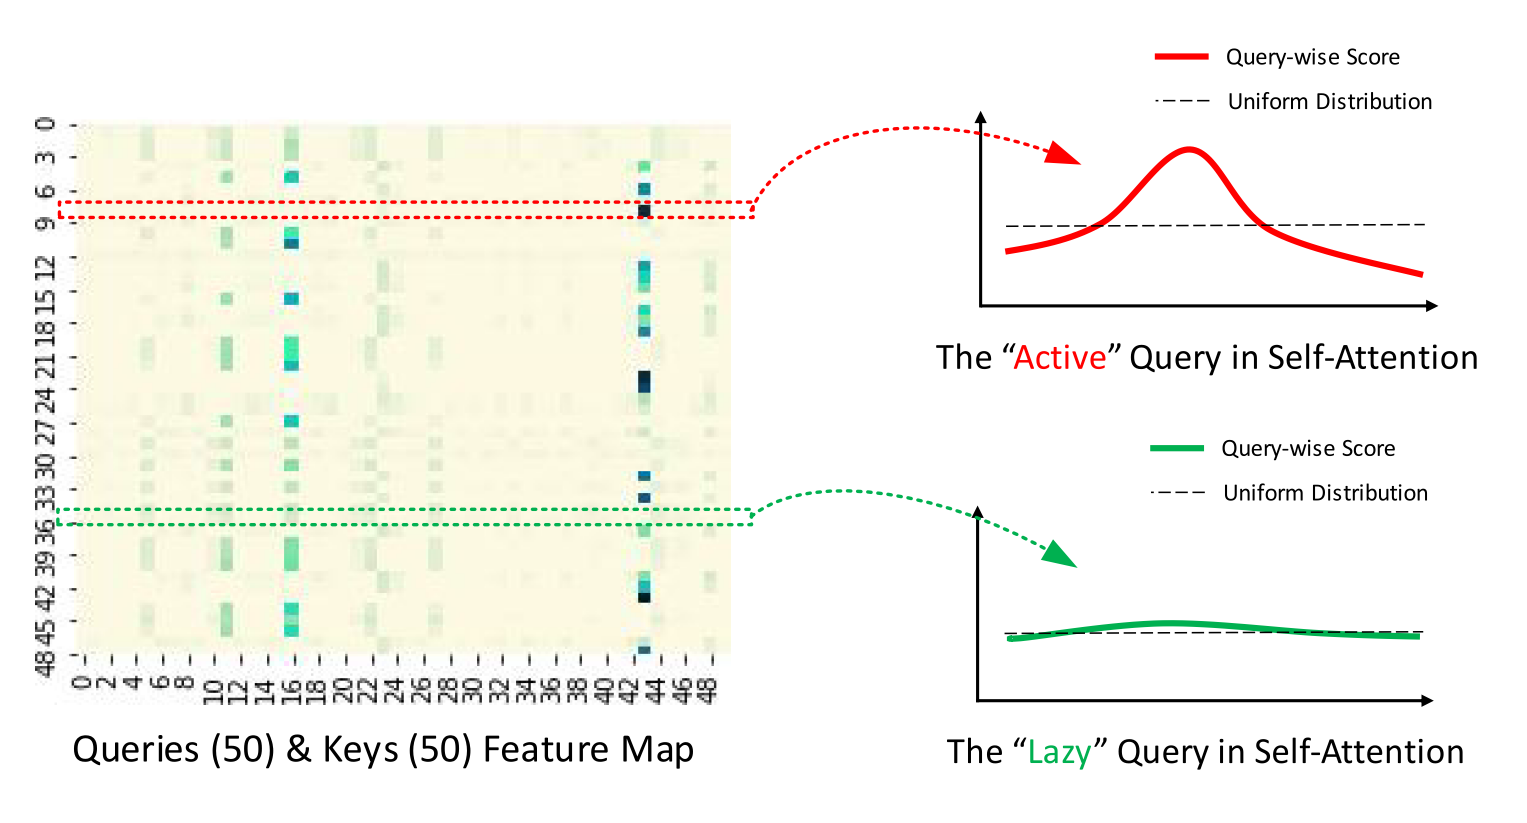
\includegraphics[width=12cm]{3_ChapterTranformerVariants/figuras/Queries_ProbSparceAttention.png}
    \caption{The illustration of ProbSparse Attention, from Informer (Zhou, et al., 2019)\cite{zhou2021informerefficienttransformerlong}}
    \LABFIG{FIG}
    \end{figure}

\subsection{Distilling}
The Informer model employs a ProbSparse self-attention mechanism, which introduces some redundancy in the encoder’s feature map. To address this, a distilling operation is used to reduce the input size between encoder layers by half, effectively removing this redundancy. In practice, the distilling operation in Informer involves adding 1D convolution layers followed by max pooling between each of the encoder layers.

Let \( X_n \) be the output of the \( n \)-th encoder layer. The distilling operation is then defined as:

\[
X_{n+1} = \text{MaxPool}(\text{ELU}(\text{Conv1d}(X_n)))
\]

By applying this operation, the input size of each subsequent layer is reduced by half. This reduction leads to a more efficient memory usage. Specifically, the memory usage is reduced from \( O(N \cdot T^2) \) to \( O(N \cdot T \log T) \), where \( N \) is the number of encoder/decoder layers and \( T \) is the sequence length. This optimization is crucial for handling long sequence time-series forecasting tasks efficiently.



%%%%%%%%%%%%%%%%%%%%%%%%%%%%%%%%%%%%%%%%%%%%%%%%%%%%%%%%%%%%%%%%
\section{Autoformer}
In June 2021, Haixu Wu, Jiehui Xu, Jianmin Wang, and Mingsheng Long introduced an innovative paper titled \textit{``Autoformer: Decomposition Transformers with Auto-Correlation for Long-Term Series Forecasting’'}. This paper has been widely recognized for its significant contributions to the field of long-term time series forecasting.

Autoformer enhances the transformer architecture by incorporating time series decomposition and a unique auto-correlation mechanism. In the following, we will explain the main contributions of Autoformer, focusing on the Decomposition Layer and the Attention (Autocorrelation) Mechanism. These innovations allow Autoformer to capture and leverage period-based dependencies, enhancing its performance over traditional transformer models.

\subsection{Decomposition Layer}
\subsubsection{Concept of Decomposition in Time Series}
Time series decomposition is a method of breaking down a time series into three systematic components: trend-cycle, seasonal variation, and random fluctuations. The trend component reflects the long-term direction of the series, which can be increasing, decreasing, or stable. The seasonal component captures recurring patterns within the series, such as yearly or quarterly cycles. The random component represents the noise that cannot be explained by the trend or seasonal components.

Decomposition can be either additive, where the components are summed, or multiplicative, where the components are multiplied. This technique, commonly implemented in libraries like \textit{statsmodels}, helps in understanding and modeling the underlying patterns in the data.

\subsubsection{Decomposition in Autoformer}
Autoformer incorporates a decomposition block within its architecture. This block enables the model to progressively aggregate the trend-cyclical part and extract the seasonal part from the series. The encoder and decoder of Autoformer use this decomposition block, significantly enhancing the model’s ability to capture and utilize these components.

Formally, for an input series \( X \in \mathbb{R}^{L \times d} \) with length \( L \), the decomposition layer returns \( X_{\text{trend}} \) and \( X_{\text{seasonal}} \) defined as:
\[
X_{\text{trend}} = \text{AvgPool}(\text{Padding}(X))
\]
\[
X_{\text{seasonal}} = X - X_{\text{trend}}
\]
This decomposition layer allows Autoformer to explicitly model the trend and seasonal components, which has proven beneficial in various time series forecasting applications.

\begin{figure}[htbp]
    \centering
    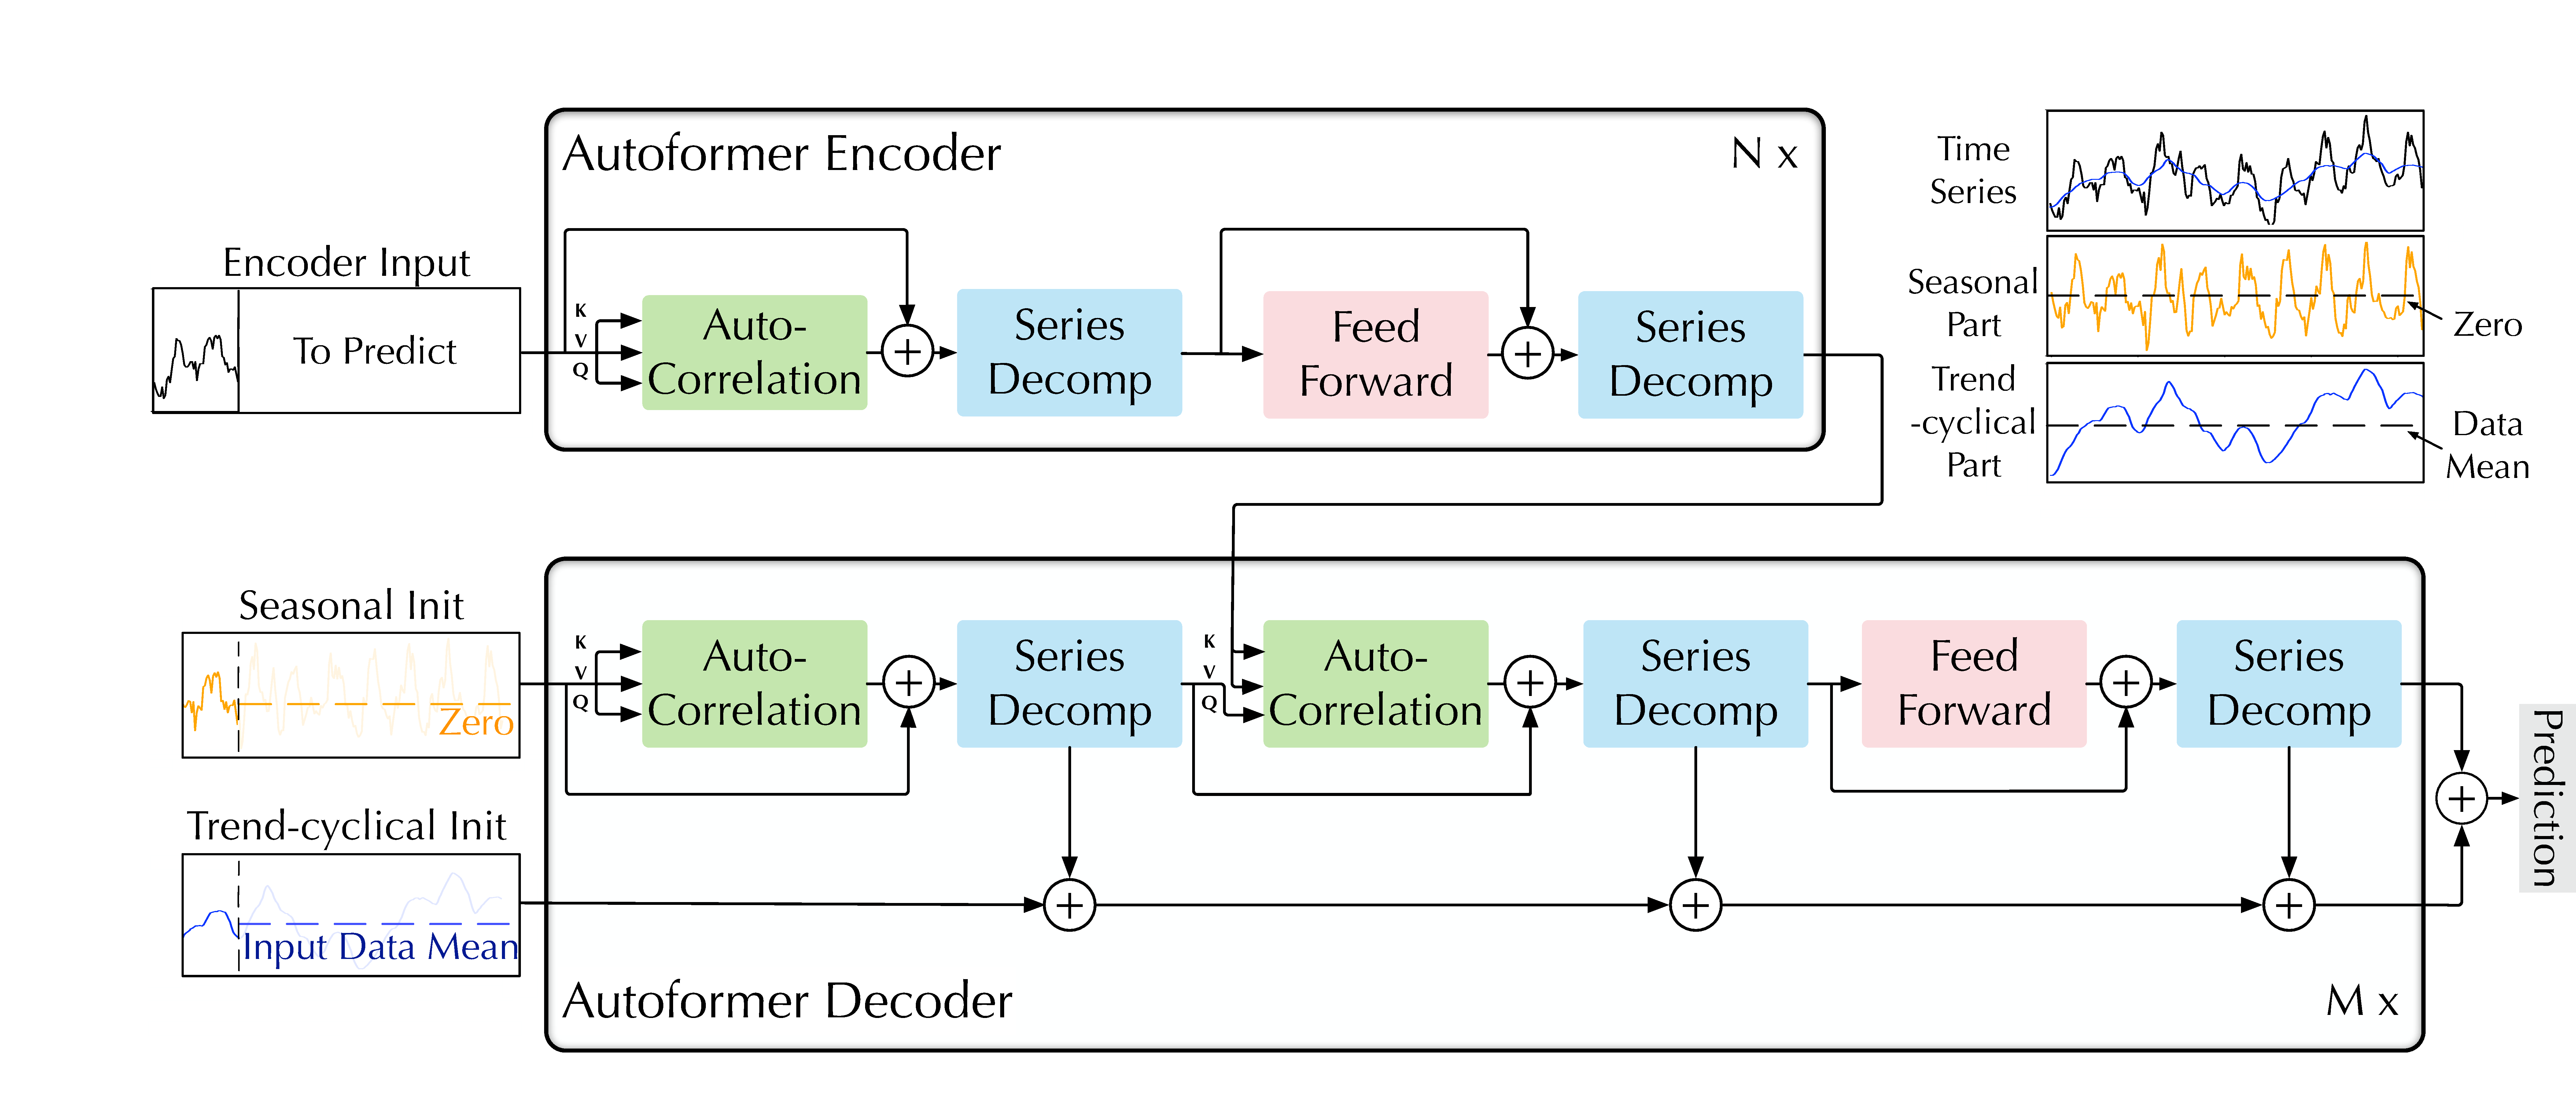
\includegraphics[width=15cm]{3_ChapterTranformerVariants/figuras/AutoformerArchitecture.pdf}
    \caption{Autoformer architecture. The encoder eliminates the long-term trend-cyclical part by series decomposition blocks (\textcolor{blue}{blue} blocks) and focuses on seasonal patterns modeling. The decoder accumulates the trend part extracted from hidden variables progressively. The past seasonal information from encoder is utilized by the encoder-decoder Auto-Correlation (center \textcolor[rgb]{0.15,0.7,0.15}{green} block in decoder), from Autoformer (Wu, Haixu, et al., 2021)\cite{wu2022autoformerdecompositiontransformersautocorrelation}}
    \LABFIG{FIG}
    \end{figure}



\subsection{Attention (Autocorrelation) Mechanism}
Autoformer introduces an innovative approach to the attention mechanism used in traditional transformers. Instead of the conventional self-attention, which calculates attention weights directly in the time domain, Autoformer utilizes an autocorrelation mechanism that operates in the frequency domain using the Fast Fourier Transform (FFT). This method helps the model better capture periodic dependencies in the data, thereby enhancing its forecasting performance.

\subsubsection{Understanding Autocorrelation}
Autocorrelation, also known as serial correlation, measures how a time series correlates with a lagged version of itself over successive time intervals. It is a crucial concept in time series analysis, as it helps identify patterns, trends, and periodic fluctuations within the data.

For a given time lag \( \tau \), autocorrelation quantifies the relationship (often measured by Pearson correlation) between the current value of the series at time \( t \) and its past value at time \( t - \tau \). Mathematically, it is expressed as:
\[
\text{Autocorrelation}(\tau) = \text{Corr}(y_t, y_{t-\tau})
\]
where \( y_t \) represents the value of the time series at time \( t \), and \( y_{t-\tau} \) represents the value at time \( t - \tau \).

Autocorrelation values range from -1 to 1:
\begin{itemize}
    \item A value of 1 indicates perfect positive correlation, meaning the series is perfectly aligned with its past values.
    \item A value of -1 indicates perfect negative correlation, meaning the series is perfectly inversely aligned with its past values.
    \item A value of 0 indicates no correlation, meaning there is no linear relationship between the current and past values.
\end{itemize}

In the context of Autoformer, this concept replaces the traditional dot-product attention mechanism used in transformers. Instead of directly comparing queries (Q) and keys (K) through dot-products, Autoformer leverages autocorrelation to capture dependencies over different time lags. This approach allows Autoformer to effectively model long-term dependencies and seasonal patterns in time series data, leading to improved forecasting performance.

\begin{figure}[htbp]
    \centering
    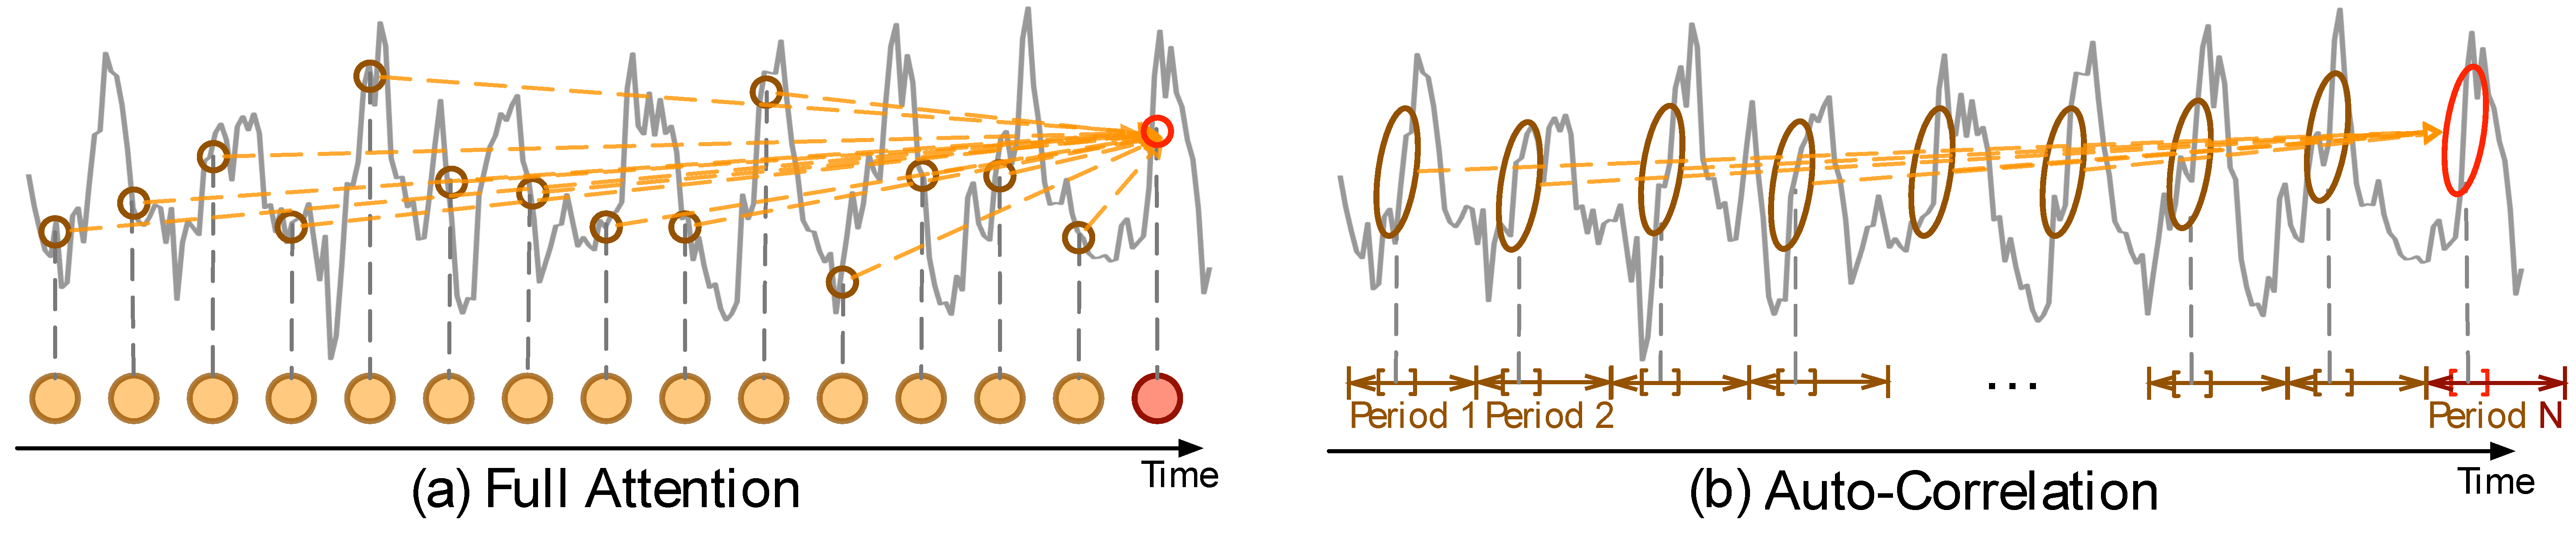
\includegraphics[width=15cm]{3_ChapterTranformerVariants/figuras/FullAttentionAutoCorrelation.pdf}
    \caption{Vanilla self attention vs Autocorrelation mechanism, from Autoformer (Wu, Haixu, et al., 2021)\cite{wu2022autoformerdecompositiontransformersautocorrelation}}
    \LABFIG{FIG}
    \end{figure}


\subsubsection{Implementing Autocorrelation with FFT}
The autocorrelation mechanism computes the attention weights using the Fast Fourier Transform (FFT). The FFT is an efficient algorithm to compute the Discrete Fourier Transform (DFT) and its inverse. It transforms a sequence of complex numbers into another sequence, representing the original sequence in the frequency domain. This approach allows all lags’ autocorrelations to be calculated simultaneously, making the process efficient with a time complexity of \( O(L \log L) \), where \( L \) is the length of the input time series.

Here’s how it works in practice:
\begin{enumerate}
    \item \textbf{FFT Transformation:} Convert the queries (Q) and keys (K) from the time domain to the frequency domain using FFT. This involves decomposing the input sequences into a sum of sinusoids of different frequencies, which represent the original data in the frequency domain.
    \item \textbf{Frequency Domain Multiplication:} Multiply the transformed Q and K element-wise in the frequency domain. This step leverages the convolution theorem, which states that convolution in the time domain corresponds to point-wise multiplication in the frequency domain.
    \item \textbf{Inverse FFT:} Apply the inverse FFT to transform the results back from the frequency domain to the time domain. This step reconstructs the autocorrelations from the frequency domain representation, yielding the desired autocorrelation values.
\end{enumerate}
    

\begin{figure}[htbp]
    \centering
    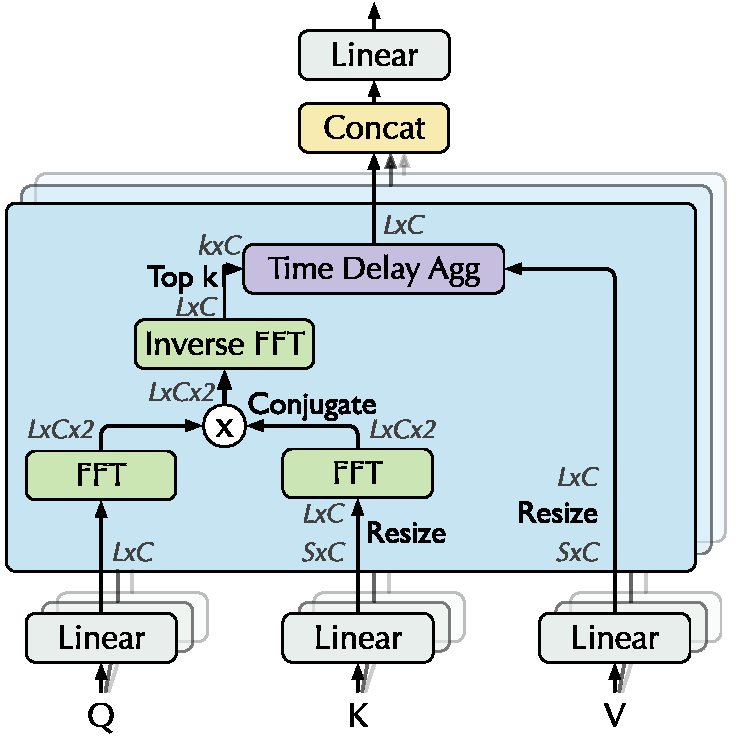
\includegraphics[width=8cm]{3_ChapterTranformerVariants/figuras/AttentionWeightsComputation.pdf}
    \caption{Attention weights computation in frequency domain using FFT, from Autoformer (Wu, Haixu, et al., 2021)\cite{wu2022autoformerdecompositiontransformersautocorrelation}}
    \LABFIG{FIG}
    \end{figure}



\subsubsection{Time Delay Aggregation}
Time Delay Aggregation (TDA) is a crucial step in the Autoformer model, designed to effectively capture the periodic dependencies in time series data. By aggregating information over different time delays, TDA ensures that the model can efficiently utilize the data, leading to better forecasting performance and improved accuracy for long-term time series forecasting.

Once the autocorrelation weights (referred to as \textit{attn\_weights}) are computed, they need to be aggregated with the values (V) to produce the final attention output. This process involves the following steps:

\begin{enumerate}
    \item \textbf{Rolling:} For each time delay \( \tau \), align the values (V) by shifting them by \( \tau \). This process is called rolling. It helps in aligning the values with their corresponding time delays, ensuring that the periodic patterns are captured accurately.
    \item \textbf{Element-wise Multiplication:} Multiply the rolled values by the corresponding autocorrelation weights. This step ensures that the influence of each time delay is weighted according to its importance, as determined by the autocorrelation weights.
    \item \textbf{Summation:} Sum the weighted values to get the final attention output. This aggregation step combines the information from different time delays, providing a comprehensive representation of the periodic dependencies in the data.
\end{enumerate}

The aggregation process can be formalized with the following equations:

\begin{enumerate}
    \item Identify the top-k lags with the highest autocorrelation values:
    \[
    \tau_1, \tau_2, \ldots, \tau_k = \text{arg Top-k}(R_{Q,K}(\tau))
    \]
    \item Apply softmax to normalize the autocorrelation values:
    \[
    \hat{R}_{Q,K}(\tau_1), \hat{R}_{Q,K}(\tau_2), \ldots, \hat{R}_{Q,K}(\tau_k) = \text{Softmax}(R_{Q,K}(\tau_1), R_{Q,K}(\tau_2), \ldots, R_{Q,K}(\tau_k))
    \]
    \item Compute the final attention output by summing the element-wise products of the rolled values and the normalized autocorrelation weights:
    \[
    \text{Autocorrelation-Attention} = \sum_{i=1}^{k} \text{Roll}(V, \tau_i) \cdot \hat{R}_{Q,K}(\tau_i)
    \]
\end{enumerate}

\begin{figure}[htbp]
    \centering
    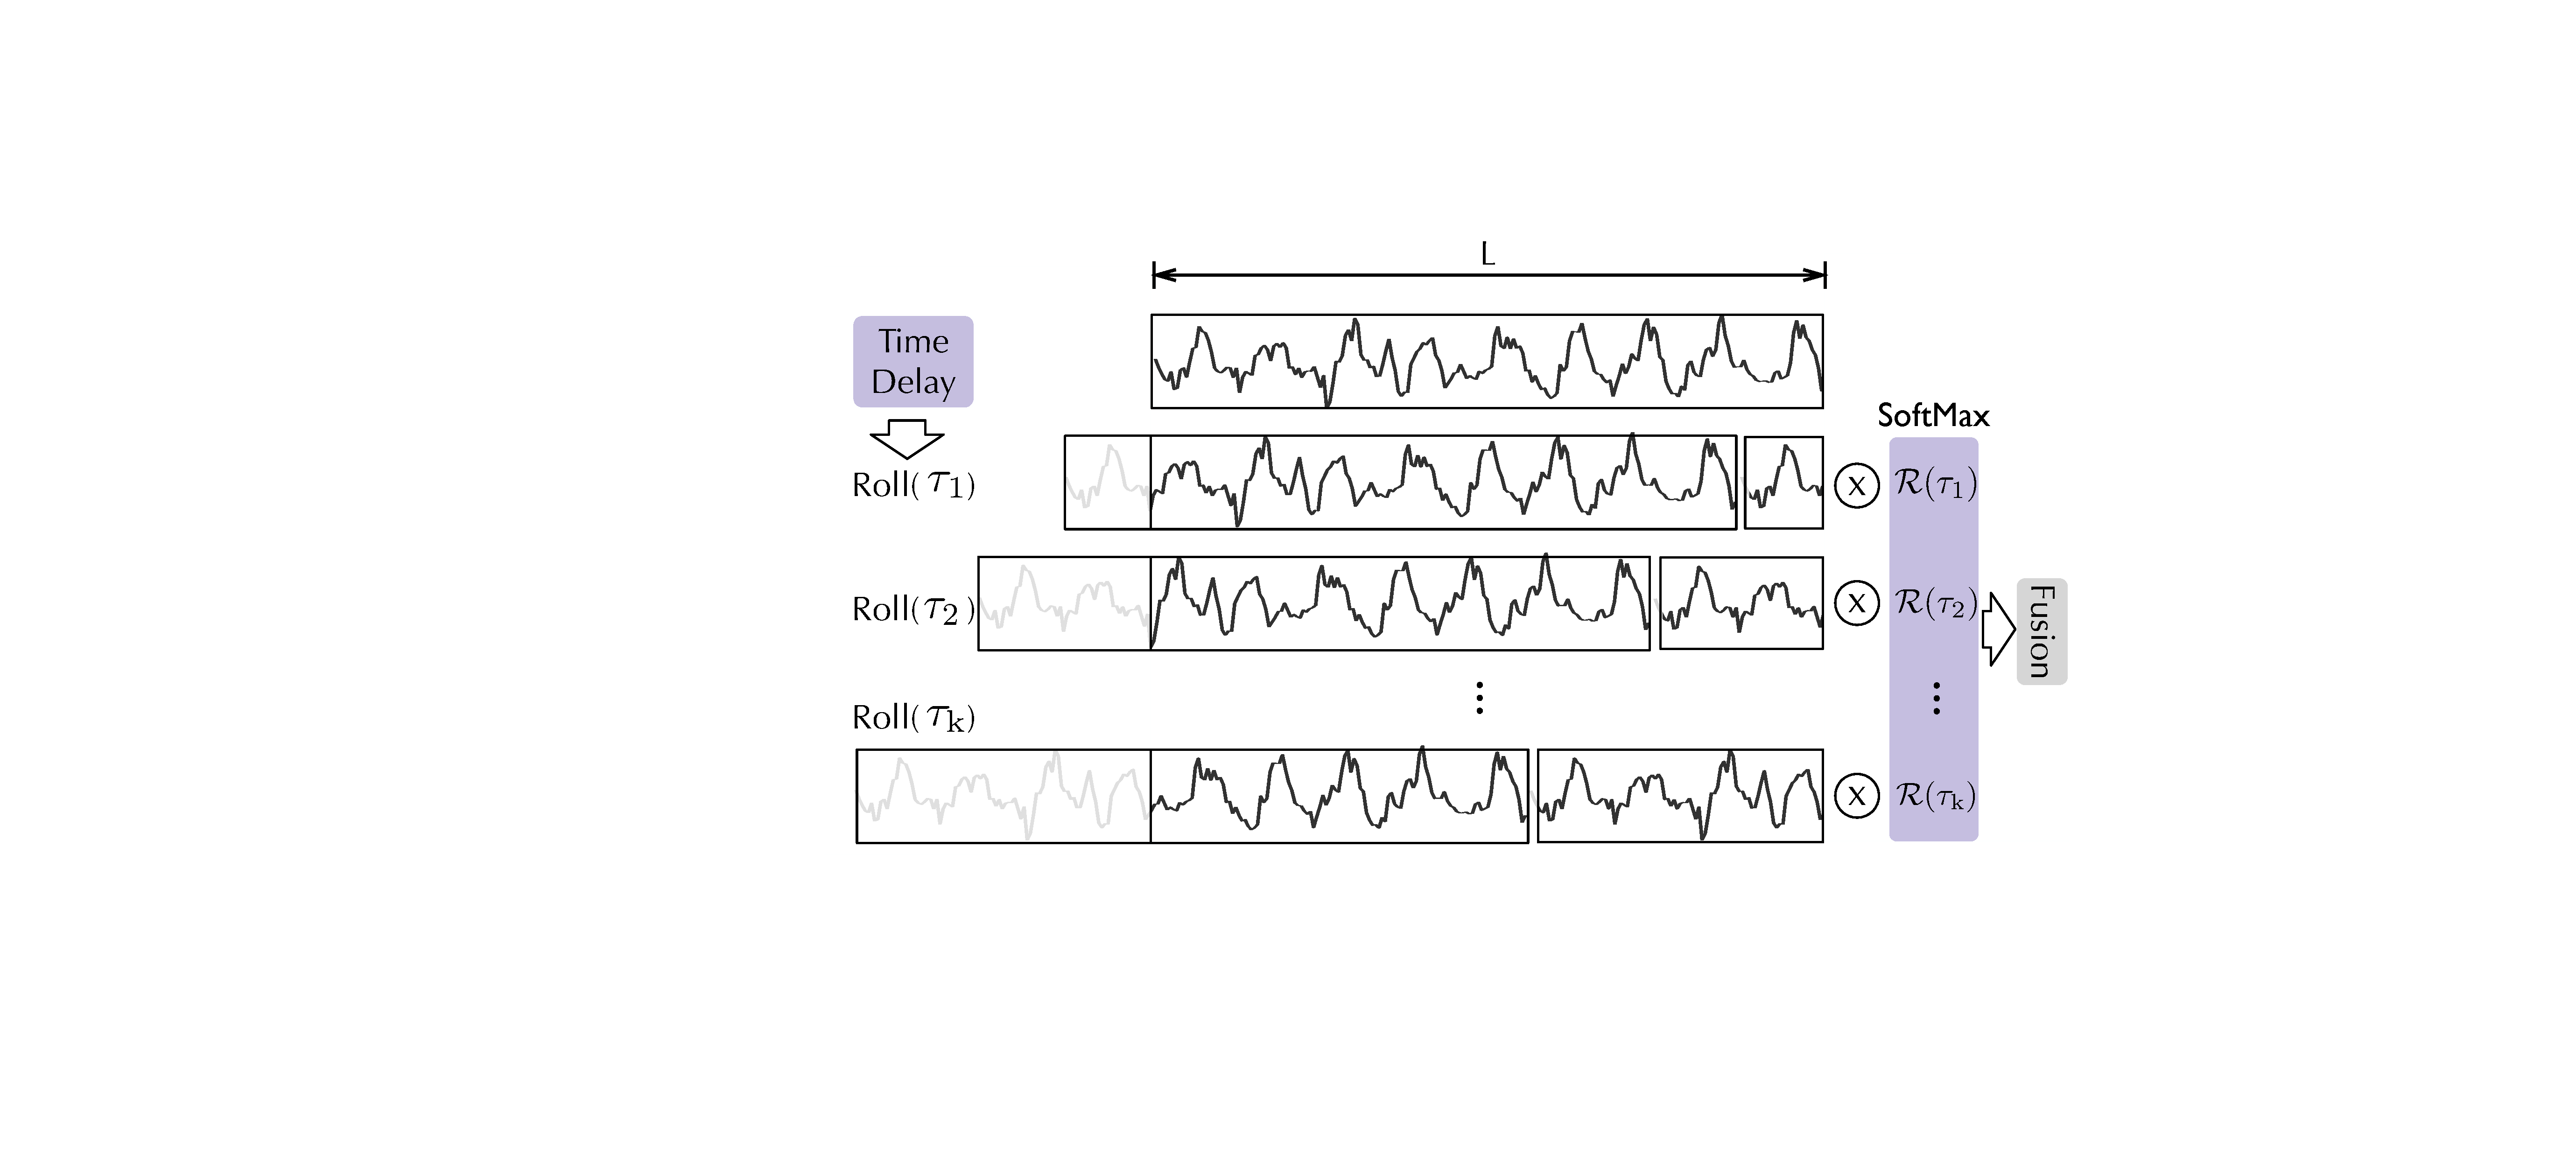
\includegraphics[width=12cm]{3_ChapterTranformerVariants/figuras/TimeDelay.pdf}
    \caption{Aggregation by time delay, from Autoformer (Wu, Haixu, et al., 2021)\cite{wu2022autoformerdecompositiontransformersautocorrelation}}
    \LABFIG{FIG}
    \end{figure}


\chapter{Materials and Methods}

\section{Datasets}

The dataset utilized in this study was provided by the supervisor and obtained by the company Ornavera. Ornavera is dedicated to generating actionable data insights for agricultural health. Their mission is to create tools for data collection in agriculture, automating mathematical and scientific processes to benefit farmers through artificial intelligence and precision agriculture.

\subsection{ORNAVERA Data Collection Device (DCD)}

The DCD is responsible for gathering and transmitting data from various geo-physical and plant sensors to the Ornavera Data Aggregation Device (DAD) using a certified LoRa® radio interface.
\begin{figure}[htbp]
    \centering
    \includegraphics[width=6 cm]{4_ChapterMaterials/figuras/DCDornavera.pdf}
    \caption{ORNAVERA Data Collection Device (DCD)\cite{ornavera2020dcd}}
    \LABFIG{FIG}
    \end{figure}

It features:
\begin{itemize}
    \item \textbf{Wireless Interface:} Utilizes LoRa® technology for long-range, low-power communication with a coverage radius of up to 15 km in rural areas and 5 km in urban areas.
    \item \textbf{Controller:} Equipped with a high-performance ARM® Cortex® microcontroller for efficient data handling and communication.
    \item \textbf{Power Supply:} Operates on a solar-assisted Li-ion battery with a backup life of 1-2 months depending on sensor usage.
    \item \textbf{Interfaces:} Supports multiple I2C, SPI, and RS485 connections for various sensors, with additional ports for future expansion.
    \item \textbf{Environmental Tolerance:} Designed to operate within a temperature range of -10°C to 55°C and humidity levels of 10\%-95\% RH.
\end{itemize}


The ORNAVERA Data Collection Device (DCD) is equipped with the following sensors:
\begin{itemize}
    \item \textbf{Temperature and Humidity Probe:} SHT20 from Sensirion, providing accurate measurements of ambient conditions around the pepper plant.
    \begin{figure}[htbp]
        \centering
        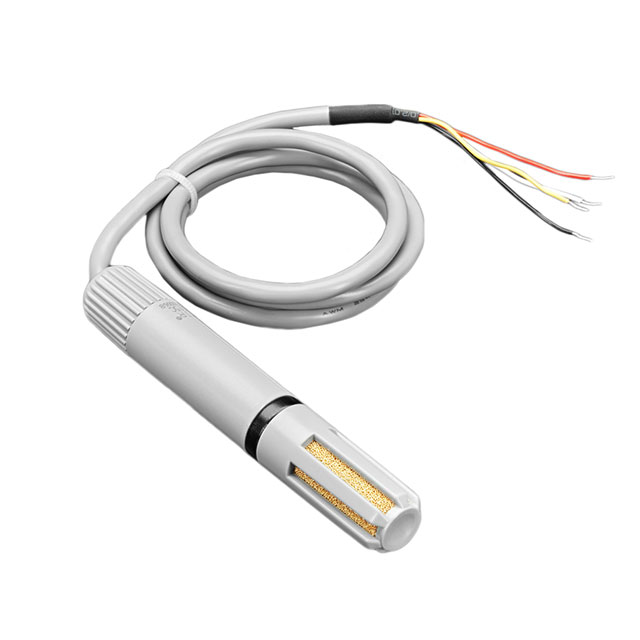
\includegraphics[width=6 cm]{4_ChapterMaterials/figuras/SHT20.jpg}
        \caption{Temperature and Humidity Probe: SHT20 from Sensirion\cite{ornavera2020dcd}}
        \LABFIG{FIG}
        \end{figure}

    \item \textbf{Soil Probe:} MEC-10, measuring soil moisture, pH, and other critical parameters for assessing soil health and suitability for pepper cultivation.
    \begin{figure}[htbp]
        \centering
        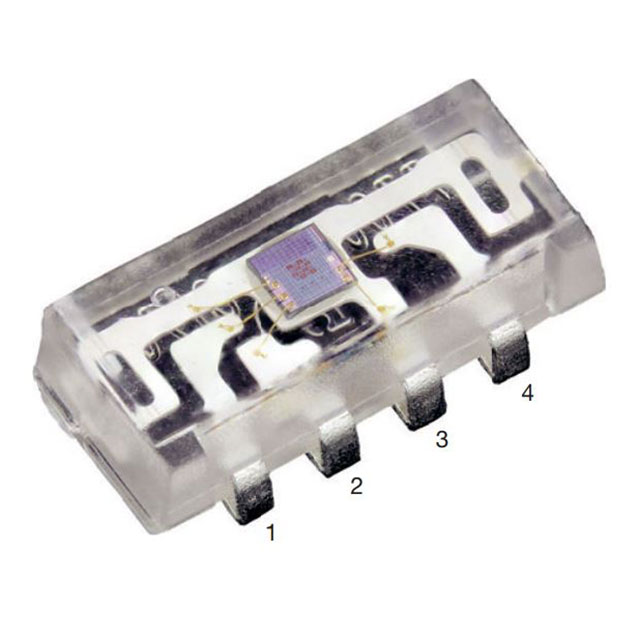
\includegraphics[width=6 cm]{4_ChapterMaterials/figuras/VEML7700.jpeg}
        \caption{Soil Probe: MEC-10 from Dalian Endeavour Technology Co. \cite{ornavera2020dcd}}
        \LABFIG{FIG}
        \end{figure}

    \item \textbf{Light Sensor:} VEML7700 from Vishay, used to measure light intensity impacting the pepper plant.
    \begin{figure}[htbp]
        \centering
        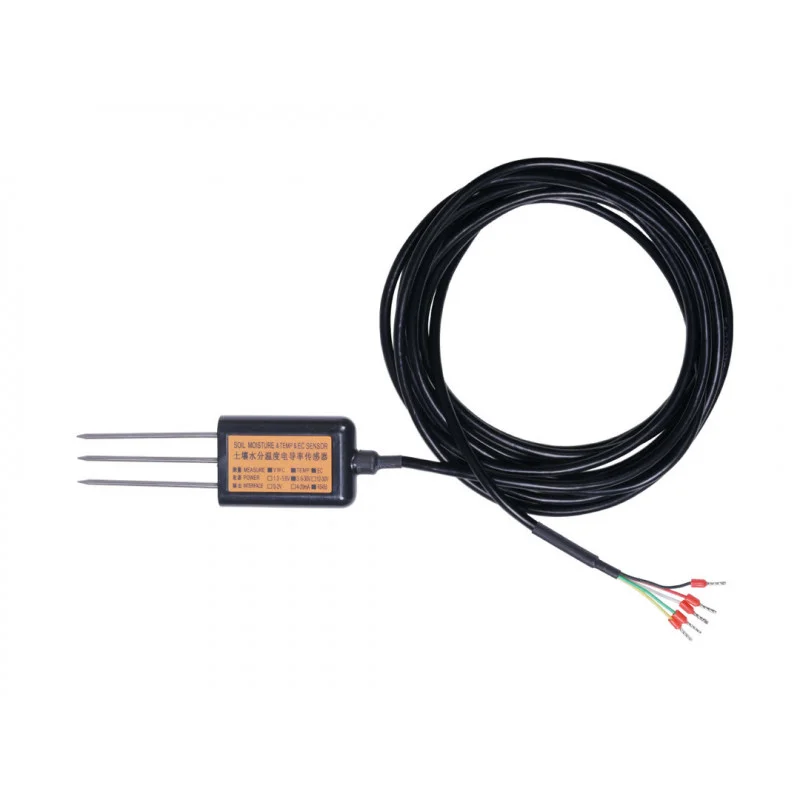
\includegraphics[width=6 cm]{4_ChapterMaterials/figuras/MEC10.png}
        \caption{Light Sensor: VEML7700 from Vishay.\cite{ornavera2020dcd}}
        \LABFIG{FIG}
        \end{figure}

    \item \textbf{Dendrometer:} Designed by Ornavera, used to measure the diameter of the pepper plant, essential for tracking its growth.
\end{itemize}


These sensors, integrated with the DCD, provided a detailed dataset for analyzing the environmental and soil conditions affecting pepper plant growth. The data collected was carefully recorded and analyzed to draw valuable insights for the study.


\section{Available Variables}

Thanks to the sensors mentioned previously, we have been able to extract a set of crucial variables for analyzing the growth of pepper plants. These data allow us to accurately assess the environmental and soil conditions that influence plant development. In the following section, the importance of these variables in plant growth is explained, highlighting how each one contributes to a better understanding of the agricultural environment and the optimization of cultivation practices.

\subsection{Temperature (t1)}

Temperature is a fundamental factor influencing plant growth, as it affects critical physiological processes such as photosynthesis, respiration, and transpiration. The variable \( t1 \) measures the ambient air temperature surrounding the plant, which is essential for determining whether environmental conditions are conducive to optimal growth. For instance, most plants have a specific temperature range within which they perform best. Outside this range, physiological processes can become less efficient, potentially leading to stress. For example, excessively high temperatures can increase respiration rates to the detriment of photosynthesis, ultimately hindering plant growth. Conversely, low temperatures can slow down metabolic activities, leading to reduced growth rates. Therefore, maintaining optimal temperature conditions can enhance the overall productivity and health of plants, making it a crucial variable to monitor.

\subsection{Relative Humidity (rh1)}

Relative humidity (\( rh1 \)) is another critical environmental factor, representing the percentage of moisture in the air relative to the maximum amount the air can hold at a given temperature. It plays a significant role in plant water use efficiency and disease management. High relative humidity can reduce transpiration rates, which might lead to an accumulation of water in the plant and potentially create conditions for disease, particularly fungal infections. Conversely, low humidity levels can cause increased transpiration, leading to water stress if not balanced by sufficient water uptake from the soil. Properly managing humidity levels is crucial for optimizing plant health, as it impacts everything from water uptake to disease resistance. Understanding relative humidity patterns allows farmers to adjust irrigation practices and greenhouse conditions to improve crop resilience and productivity.

\subsection{Vapor Pressure Deficit (vpd1)}

Vapor Pressure Deficit (VPD), derived from relative humidity and temperature, provides insights into the drying power of the air. It represents the difference between the amount of moisture in the air and how much moisture the air can hold when saturated. This measure is crucial for understanding plant transpiration rates and water stress levels. High VPD indicates drier air, which can increase transpiration and potentially lead to water stress if not adequately managed. On the other hand, low VPD suggests more humid conditions, which can reduce transpiration and, in some cases, lead to an excess of moisture around the plant, fostering mold and mildew. By monitoring VPD, growers can make informed decisions about irrigation and climate control, ensuring plants receive the optimal balance of moisture to thrive.

\subsection{Light Intensity (lux)}

Light intensity, measured in lumens (lux), is crucial for plant growth as it directly impacts photosynthesis—the process by which plants convert light into energy. Adequate light intensity is essential for driving this process, influencing growth rates and overall plant health. Insufficient light can limit photosynthesis, stunting growth and leading to weaker plants, while excessive light can cause photoinhibition, where too much light actually damages the photosynthetic apparatus, reducing efficiency. Understanding and managing light exposure is therefore vital for maximizing photosynthetic activity, especially in controlled environments like greenhouses. By ensuring that plants receive the right amount of light, farmers can enhance growth rates, improve flowering and fruiting patterns, and optimize crop yields.

\subsection{Soil Temperature (st1)}

Soil temperature (\( st1 \)) is a key variable that influences root activity and microbial processes in the soil, both of which are critical for nutrient uptake and plant growth. Soil temperature affects root metabolism, with optimal temperatures promoting vigorous root growth and nutrient absorption. If soil temperatures fall outside the optimal range, root activity can slow down, impairing the plant's ability to access water and nutrients, and potentially leading to stunted growth. Additionally, soil temperature affects the activity of soil microbes, which play a vital role in decomposing organic matter and releasing nutrients in forms that plants can absorb. Monitoring soil temperature helps in managing planting schedules and optimizing root zone conditions to ensure that plants have access to the nutrients they need for healthy growth and development.

\subsection{Permittivity (p1)}

Permittivity is a measure of a soil's ability to store and transmit electric fields, closely related to its moisture content. High permittivity often indicates a higher soil moisture level, which is crucial for nutrient transport and root uptake. Adequate soil moisture facilitates the movement of nutrients from the soil to the plant roots, thereby supporting healthy growth. However, too much moisture can lead to waterlogged conditions, which can suffocate roots and inhibit their ability to function properly. By measuring permittivity, growers can gain insights into soil moisture levels and make informed decisions about irrigation practices. This ensures that plants receive the optimal amount of water, reducing stress and enhancing growth conditions, which is particularly important for maintaining crop health in varying weather conditions.

\subsection{Electrical Conductivity (ec1)}

Electrical conductivity (\( ec1 \)) measures the soil's ability to conduct electricity, which is indicative of the concentration of soluble salts and nutrients in the soil. High electrical conductivity can indicate excessive salts, which may lead to osmotic stress and interfere with nutrient uptake. This can harm plant growth, especially in crops sensitive to salinity. On the other hand, low electrical conductivity may suggest nutrient deficiencies that can limit growth and yield. Monitoring electrical conductivity is essential for diagnosing soil fertility and salinity issues, allowing farmers to adjust fertilization practices accordingly. By maintaining balanced nutrient levels, plants can achieve optimal growth and productivity, highlighting the importance of regular soil EC monitoring.

\subsection{Volumetric Water Content (vwc1)}

Volumetric Water Content (\( vwc1 \)) measures the percentage of water present in the soil, reflecting the soil moisture status and availability for plant uptake. This variable is crucial for understanding the water dynamics within the soil and ensuring plants have sufficient water for physiological processes. Adequate soil moisture supports nutrient uptake and maintains plant turgor, which is vital for growth and stability. However, both insufficient and excessive moisture can cause stress: too little water can lead to drought stress, while too much can lead to root rot and decreased oxygen availability. By monitoring volumetric water content, growers can fine-tune irrigation practices to maintain optimal soil moisture levels, improving plant health, conserving water, and ensuring efficient use of resources.

\subsection{Diameter (diam1)}

The diameter of a plant's stem (\( diam1 \)) serves as a practical measure of its growth vigor and overall health. An increasing diameter generally indicates healthy growth and biomass accumulation, reflecting the plant's ability to assimilate nutrients and convert them into structural tissues. Consistent monitoring of stem diameter can reveal growth trends and potentially highlight stress conditions before they become severe. For instance, a sudden decrease in growth rate might indicate a nutrient deficiency, water stress, or pest problem. Additionally, a thicker stem provides better structural support for the plant, enabling it to withstand environmental stresses and support fruit load. By measuring changes in diameter, farmers can assess plant health and make timely interventions to support optimal growth conditions.

\subsection{Photosynthetically Active Radiation (par)}

Photosynthetically Active Radiation (PAR) is the portion of the light spectrum (400-700 nm) that plants use for photosynthesis. Unlike total light intensity, PAR specifically measures the wavelengths that drive photosynthesis, making it a more precise indicator of the light energy available for plant growth. The amount of PAR a plant receives directly influences its photosynthetic efficiency and, consequently, its growth and productivity. Variations in PAR can affect plant morphology, influencing factors such as leaf size, stem elongation, and flowering. By monitoring PAR, growers can optimize light conditions to ensure maximum photosynthetic activity, particularly in controlled environments like greenhouses where artificial lighting may be used. This helps in enhancing growth rates and improving yield quality, underscoring the importance of precise light management.

\chapter{Experimental Design}

\section{Dataset Preprocessing}

This section describes the preprocessing steps applied to the time series datasets used in this study. Initially, we had access to four different datasets: two containing measurements taken on sand and two on clay. Each dataset included various variables representing different environmental conditions and characteristics. However, during the data exploration phase, significant inconsistencies were identified in three of the datasets.

The errors detected included abrupt increases in the values of certain variables from one day to the next. In the sand datasets, it was observed that for diameter measurements, the values unexpectedly doubled or tripled overnight. This phenomenon could be explained by a possible change of sensors, which might have altered the measurements without prior notice.

\begin{figure}[htbp]
    \centering
    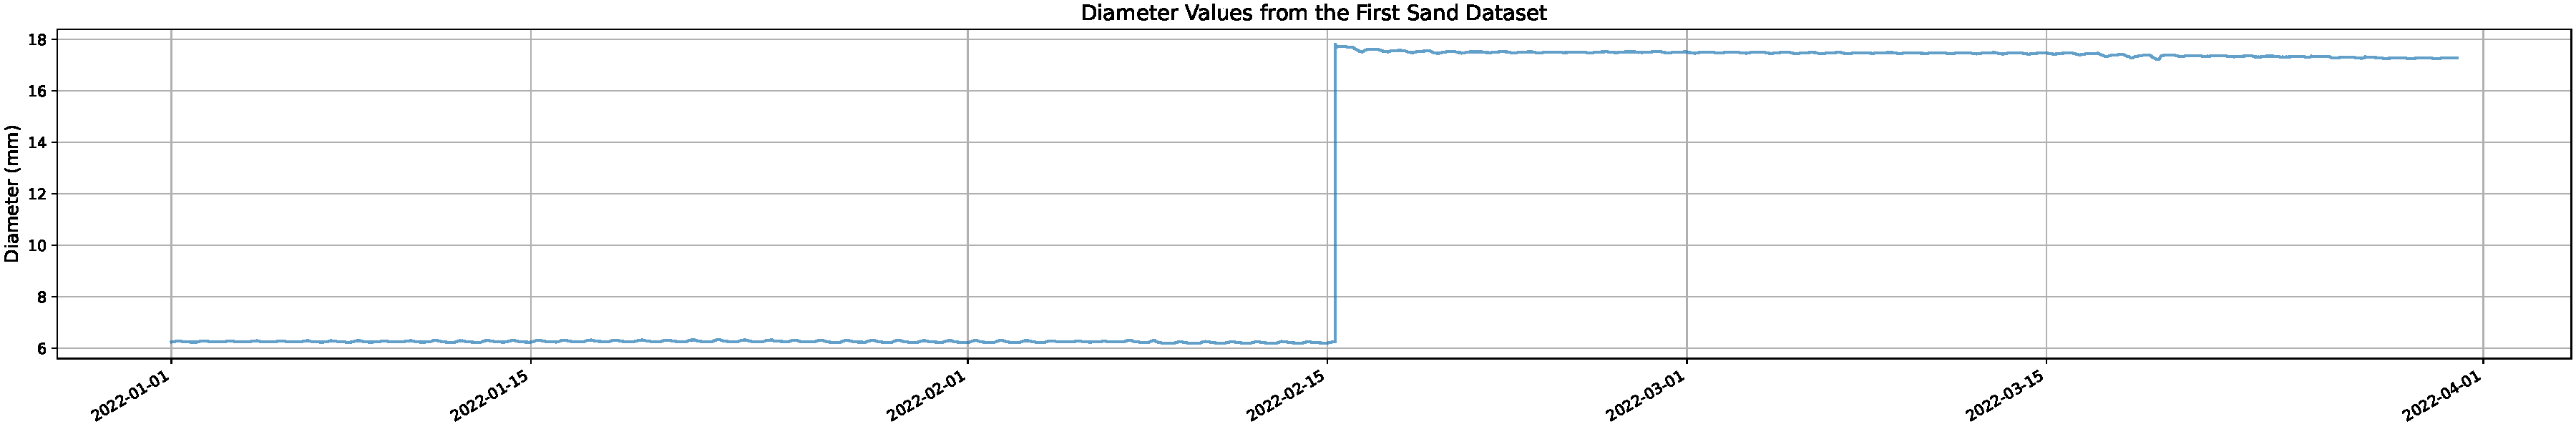
\includegraphics[width=15 cm]{5_ChapterDesign/figuras/1_DatasetIssues/Diameter_Sand_1}
    \caption{Example of Diameter Measurement Error in the First Sand Dataset}
    \LABFIG{FIG}
    \end{figure}

Similarly, the data related to light intensity showed sudden variations in lumens. In this case, it is likely that the sensor was either cleaned or repositioned, which could have caused a significant change in light measurements from one day to the next. The following image illustrates an example of these abrupt changes:

\begin{figure}[htbp]
    \centering
    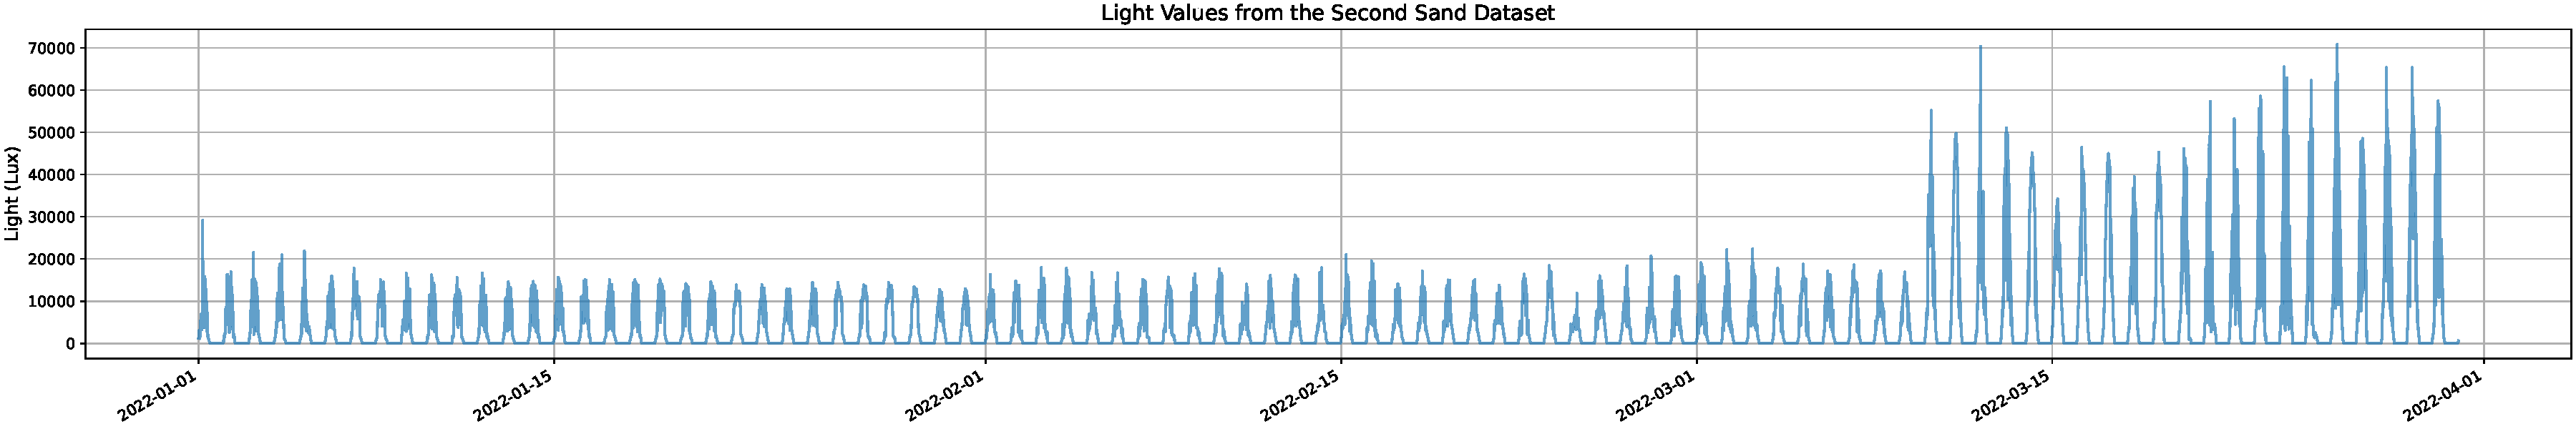
\includegraphics[width=15 cm]{5_ChapterDesign/figuras/1_DatasetIssues/Light_Sand_2}
    \caption{Example of Light Measurement Error in the Second Sand Dataset}
    \LABFIG{FIG}
    \end{figure}

Due to these inconsistencies and after a thorough evaluation of the data, we decided to use one of the clay datasets, which presented more reasonable and consistent measurements over time. This dataset was selected for further analysis as it offered a more stable and reliable framework for studying time series data.

However, even the selected dataset required significant preprocessing to transform its structure and ensure data quality. This preprocessing process included steps such as normalizing values, handling missing data, and removing potential outliers. The detailed steps carried out in this phase are presented below.

\subsection{Structure}

The initial dataset provided by Ornavera was in the \texttt{.mat} format, which is commonly used for MATLAB. To facilitate data analysis and manipulation in Python, it was necessary to convert this data into a \texttt{.csv} file format. This conversion was advantageous because \texttt{.csv} files are universally supported and can be easily imported into Python libraries such as Pandas, making data manipulation and analysis straightforward. Additionally, CSV files are text-based, making them easy to inspect and modify with a simple text editor, and they offer efficiency benefits for large datasets due to their simple structure, which can be quickly parsed by Python libraries.

To perform the conversion, we wrote a MATLAB function named \texttt{mat\_to\_csv}, which loads the data from the \texttt{.mat} file, eliminates unnecessary fields, and writes the cleaned data to a \texttt{.csv} file. The function specifically targeted fields that were not relevant to our analysis, such as various identifiers and redundant measurements. Removing these fields helped streamline the dataset, ensuring that it was focused on the variables that were of interest for our study.

\begin{lstlisting}[language=Matlab,caption={MATLAB function to convert .mat file to .csv}, label=lst:mat_to_csv]
function mat_to_csv(mat_file, csv_file)
    % Load the data from the .mat file
    load(mat_file, 'val');
    
    % Eliminate the fields we are not interested in
    fields_to_eliminate = {'rid', 'cid','lid','vpd1','dd1','wtlux','alux','ecb1','ecp1','st2', 'p2', 'ec2', 'vwc2', 'ecb2', 'ecp2', 'st3', 'p3', 'ec3', 'vwc3', 'ecb3', 'ecp3','par','dli'};
    val_cleaned = val; % Create a copy of the original structure
    for i = 1:numel(fields_to_eliminate)
        val_cleaned = rmfield(val_cleaned, fields_to_eliminate{i});
    end
    
    % Convert the data from a structure to a table
    val_table = struct2table(val_cleaned);
    
    % Change the field names of the table
    new_names = {'Identificator', 'Date', 'Month','Day','Year','Hour','Minute','Second','Temperature','Relative_humidity', 'Light', 'Soil_temperature', 'Permittivity', 'Electroconductivity', 'Volumetric_water_content', 'Diameter', 'Battery_voltage'};
    val_table.Properties.VariableNames = new_names;
    
    % Write the data to a .csv file
    writetable(val_table, csv_file, 'Delimiter', ';');
end
\end{lstlisting}

The code effectively transformed the data from a complex structure into a more usable format by converting it into a table and renaming the fields to be more descriptive. The \texttt{.csv} file was then generated with a delimiter suitable for easy parsing in Python. This preparation step was crucial in setting the stage for efficient data handling and analysis in the subsequent phases of the project.

\subsection{Signal smoothing}

To achieve the signal smoothing, we use a Savitzky-Golay filter with a window size of 11 and a polynomial order of 2. In this case, we start with the data signal after removing the initial slope. The window size is set to 11, meaning that 11 adjacent data points are used to calculate each smoothed value. This implies that the filter takes these 11 points and fits a second-degree polynomial, also known as a parabola, to the data within each window, allowing the signal to be smoothed without losing its essential characteristics.

The \texttt{savgol\_filter} function generates a smoothed version of the input signal. By applying this filter, the smoothed signal exhibits a significant reduction in noise, making it more continuous and less fluctuating than the original signal. The smoothing process enhances the visualization and analysis of the underlying trends in the data, allowing important features to stand out more clearly. This can be clearly observed in the graphs presented below.


\begin{figure}[htbp]
    \centering
    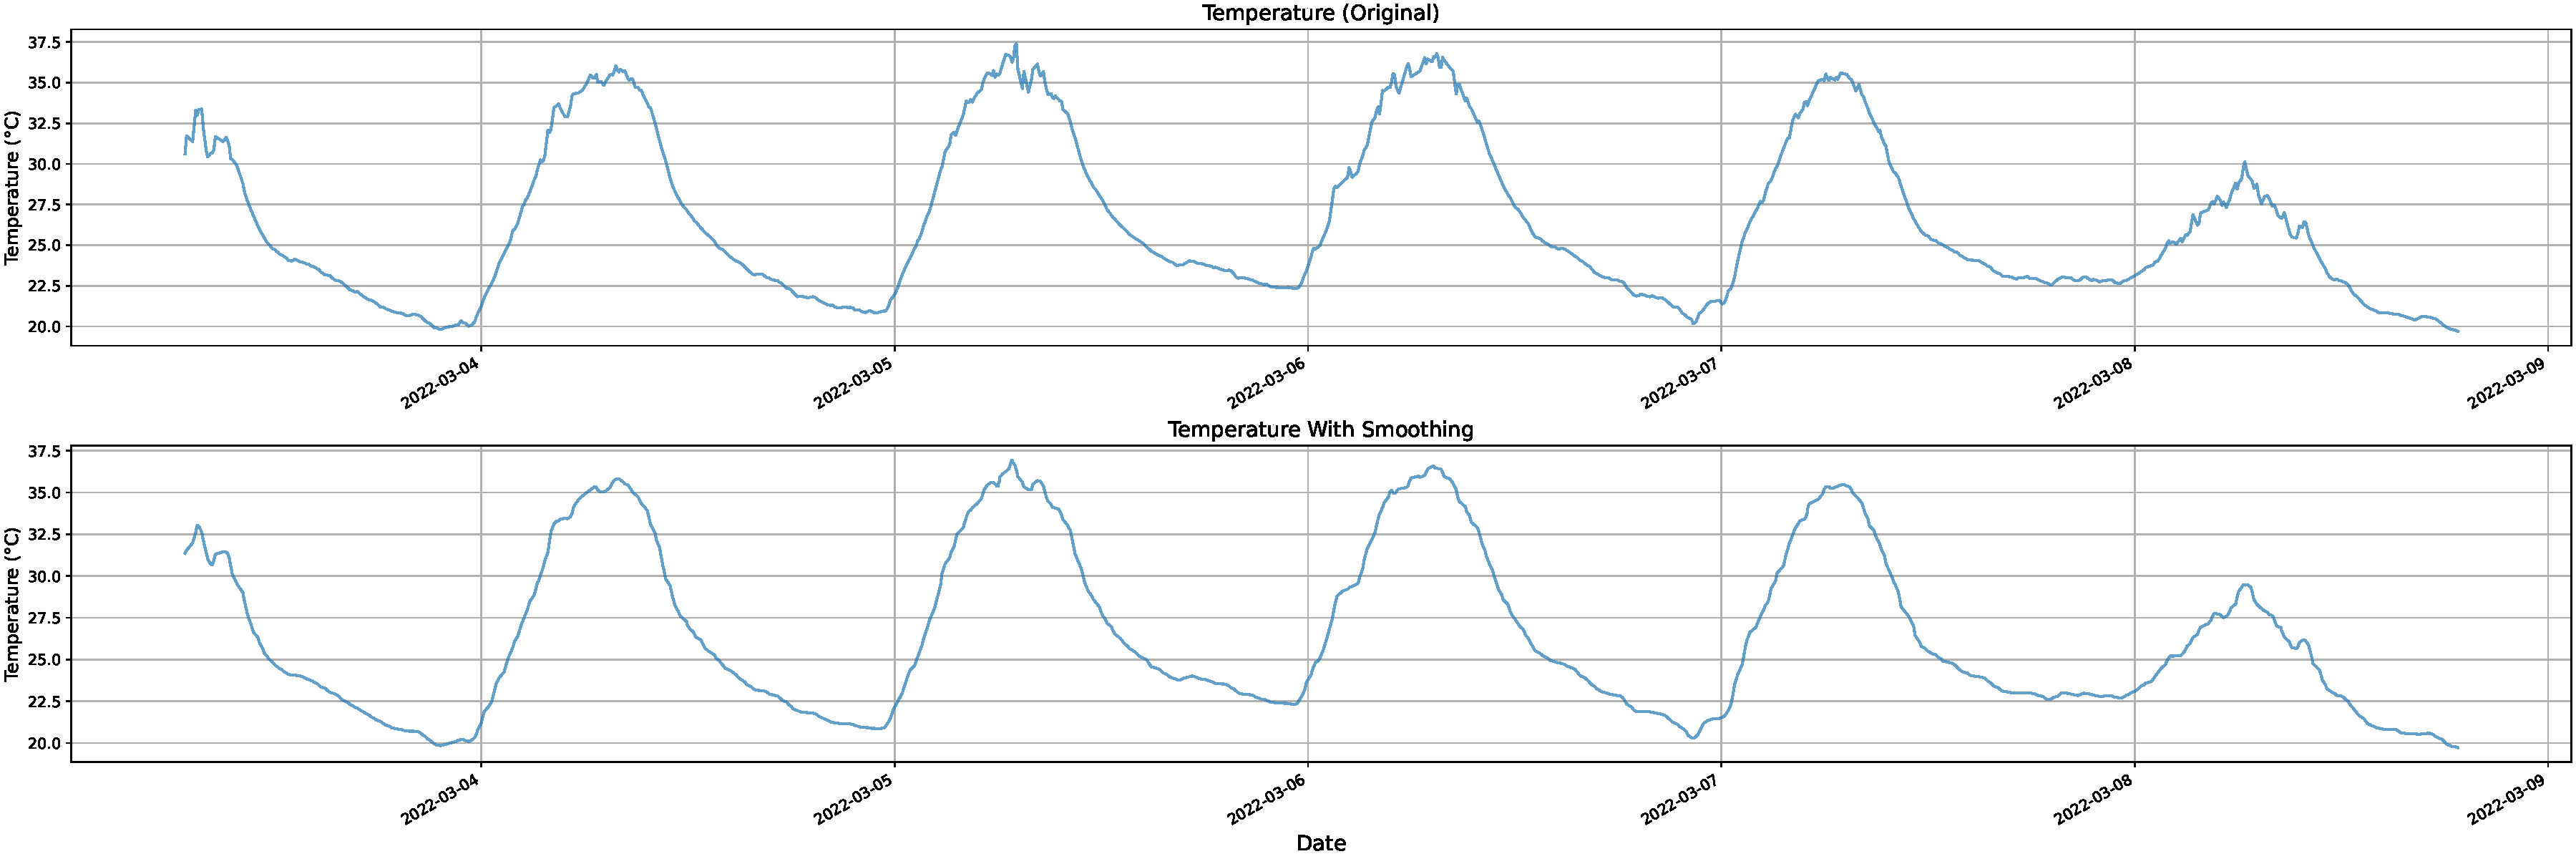
\includegraphics[width=15 cm]{5_ChapterDesign/figuras/2_Smoothing/Smoothing_Temperature}
    \caption{Original Temperature data (top) versus the Temperature smoothed data (bottom) after applying a Savitzky-Golay filter}
    \LABFIG{FIG}
\end{figure}

\begin{figure}[htbp]
    \centering
    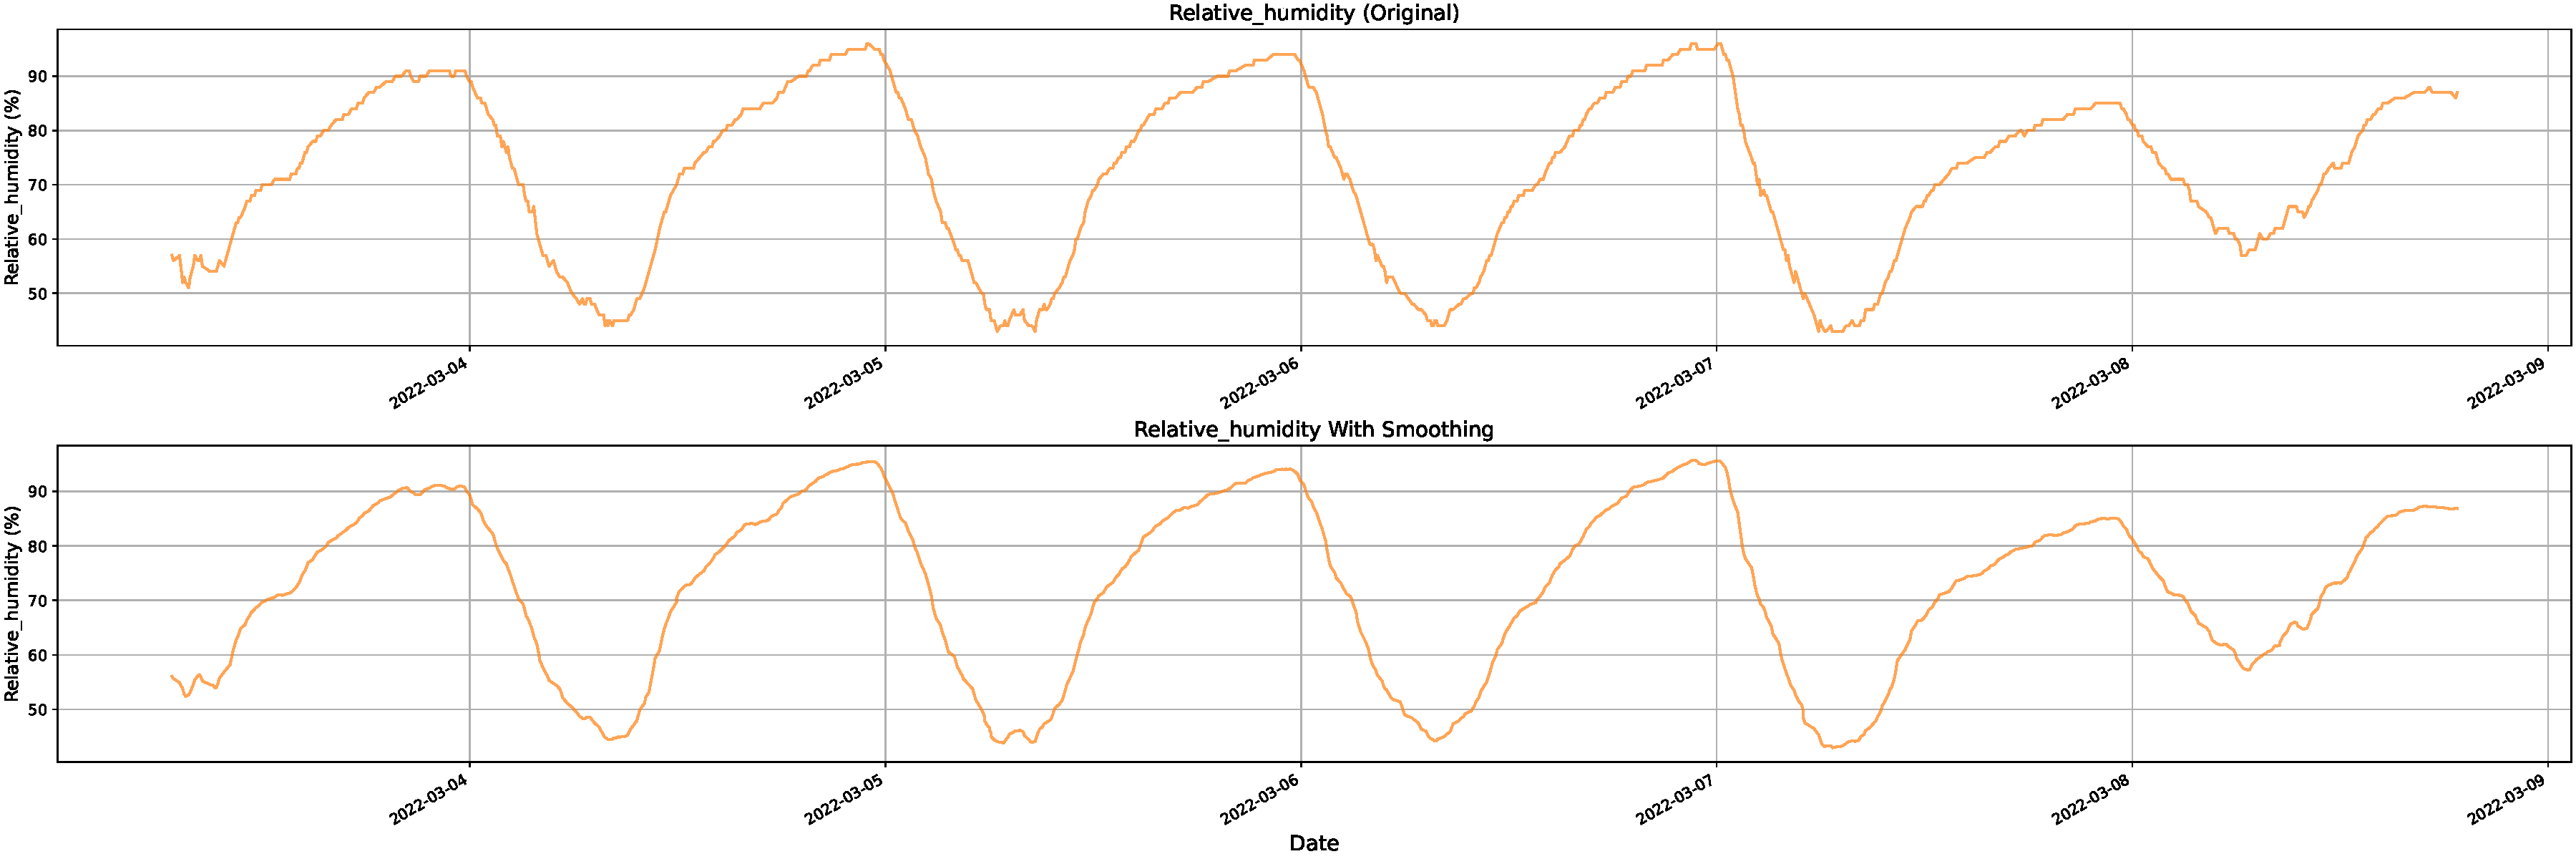
\includegraphics[width=15 cm]{5_ChapterDesign/figuras/2_Smoothing/Smoothing_Relative_humidity}
    \caption{Original Relative humidity data (top) versus the Relative humidity smoothed data (bottom) after applying a Savitzky-Golay filter}
    \LABFIG{FIG}
\end{figure}

\begin{figure}[htbp]
    \centering
    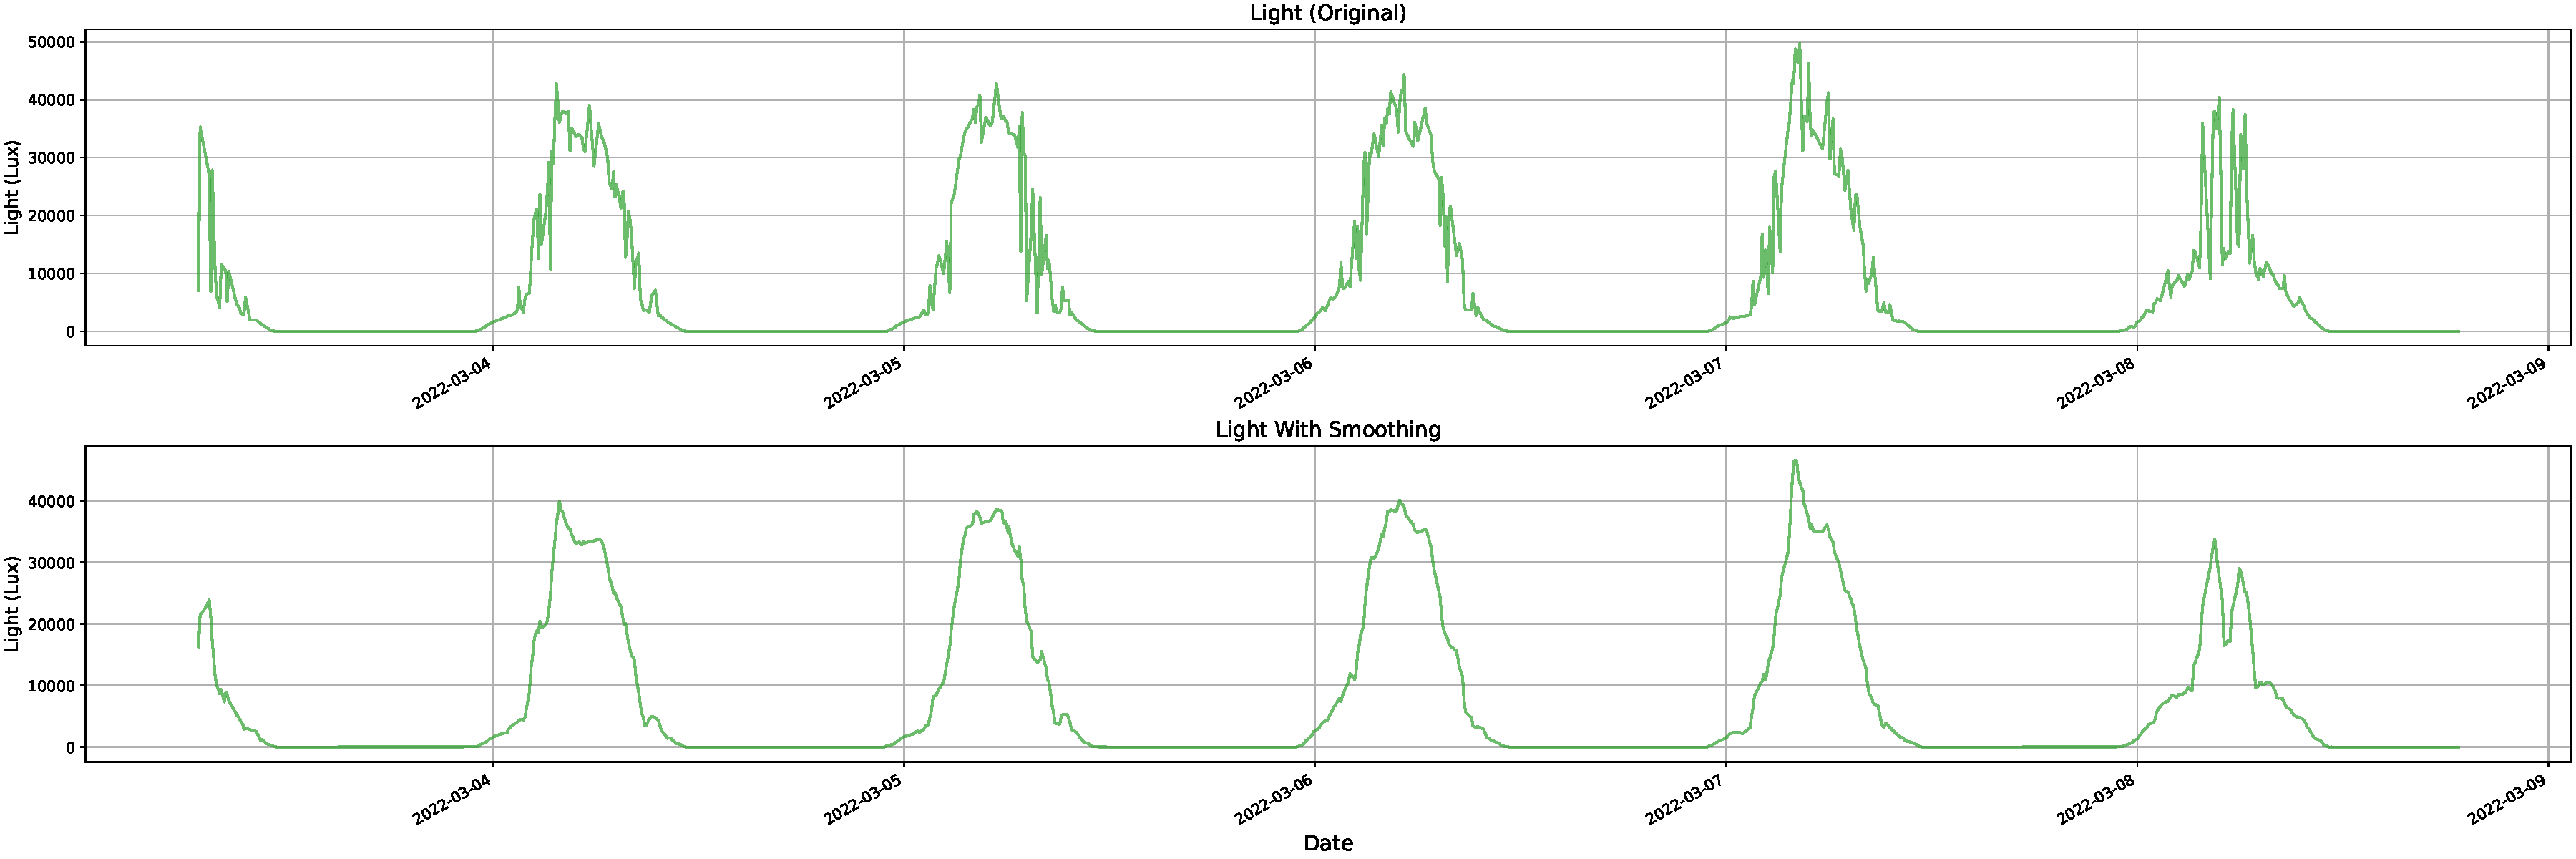
\includegraphics[width=15 cm]{5_ChapterDesign/figuras/2_Smoothing/Smoothing_Light}
    \caption{Original Light data (top) versus the Light smoothed data (bottom) after applying a Savitzky-Golay filter}
    \LABFIG{FIG}
\end{figure}

\begin{figure}[htbp]
    \centering
    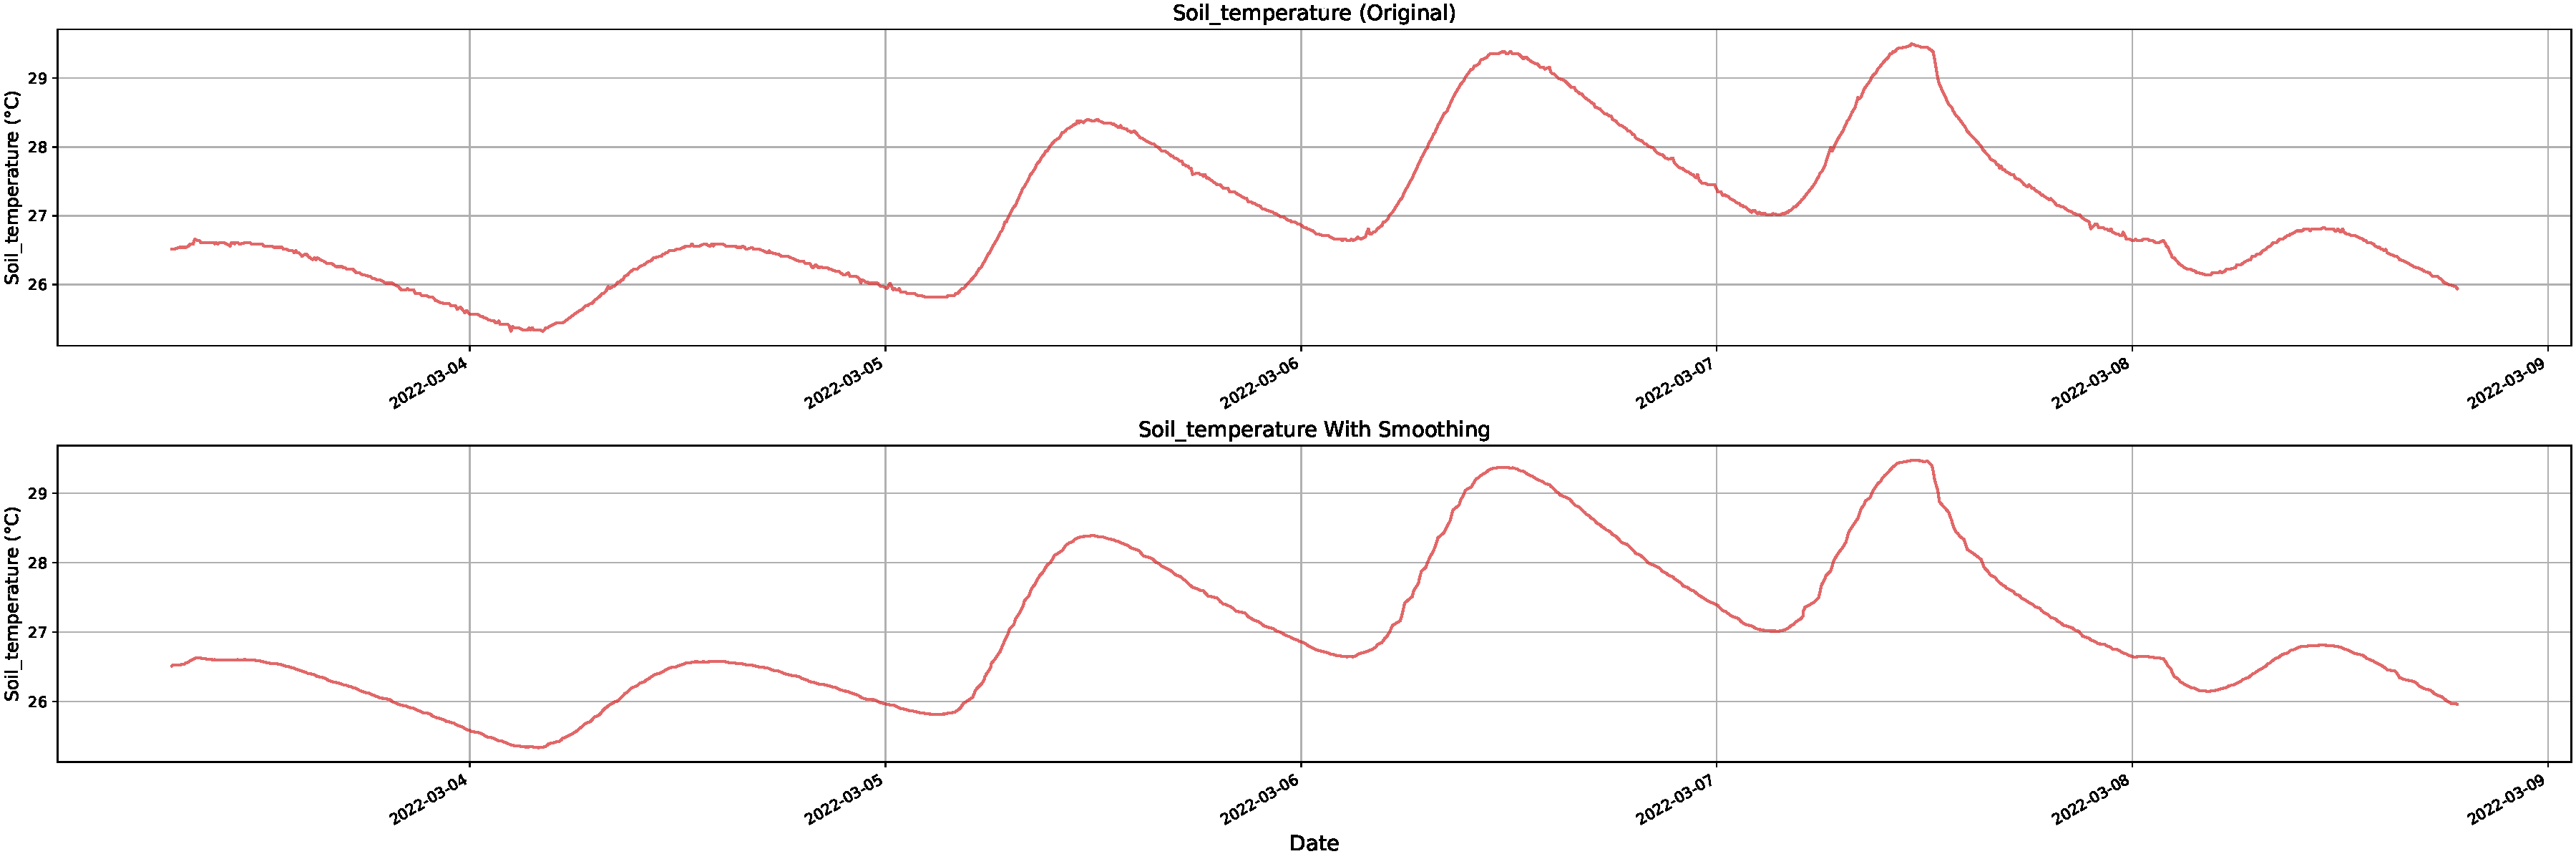
\includegraphics[width=15 cm]{5_ChapterDesign/figuras/2_Smoothing/Smoothing_Soil_temperature}
    \caption{Original Soil temperature data (top) versus the Soil temperature smoothed data (bottom) after applying a Savitzky-Golay filter}
    \LABFIG{FIG}
\end{figure}

\begin{figure}[htbp]
    \centering
    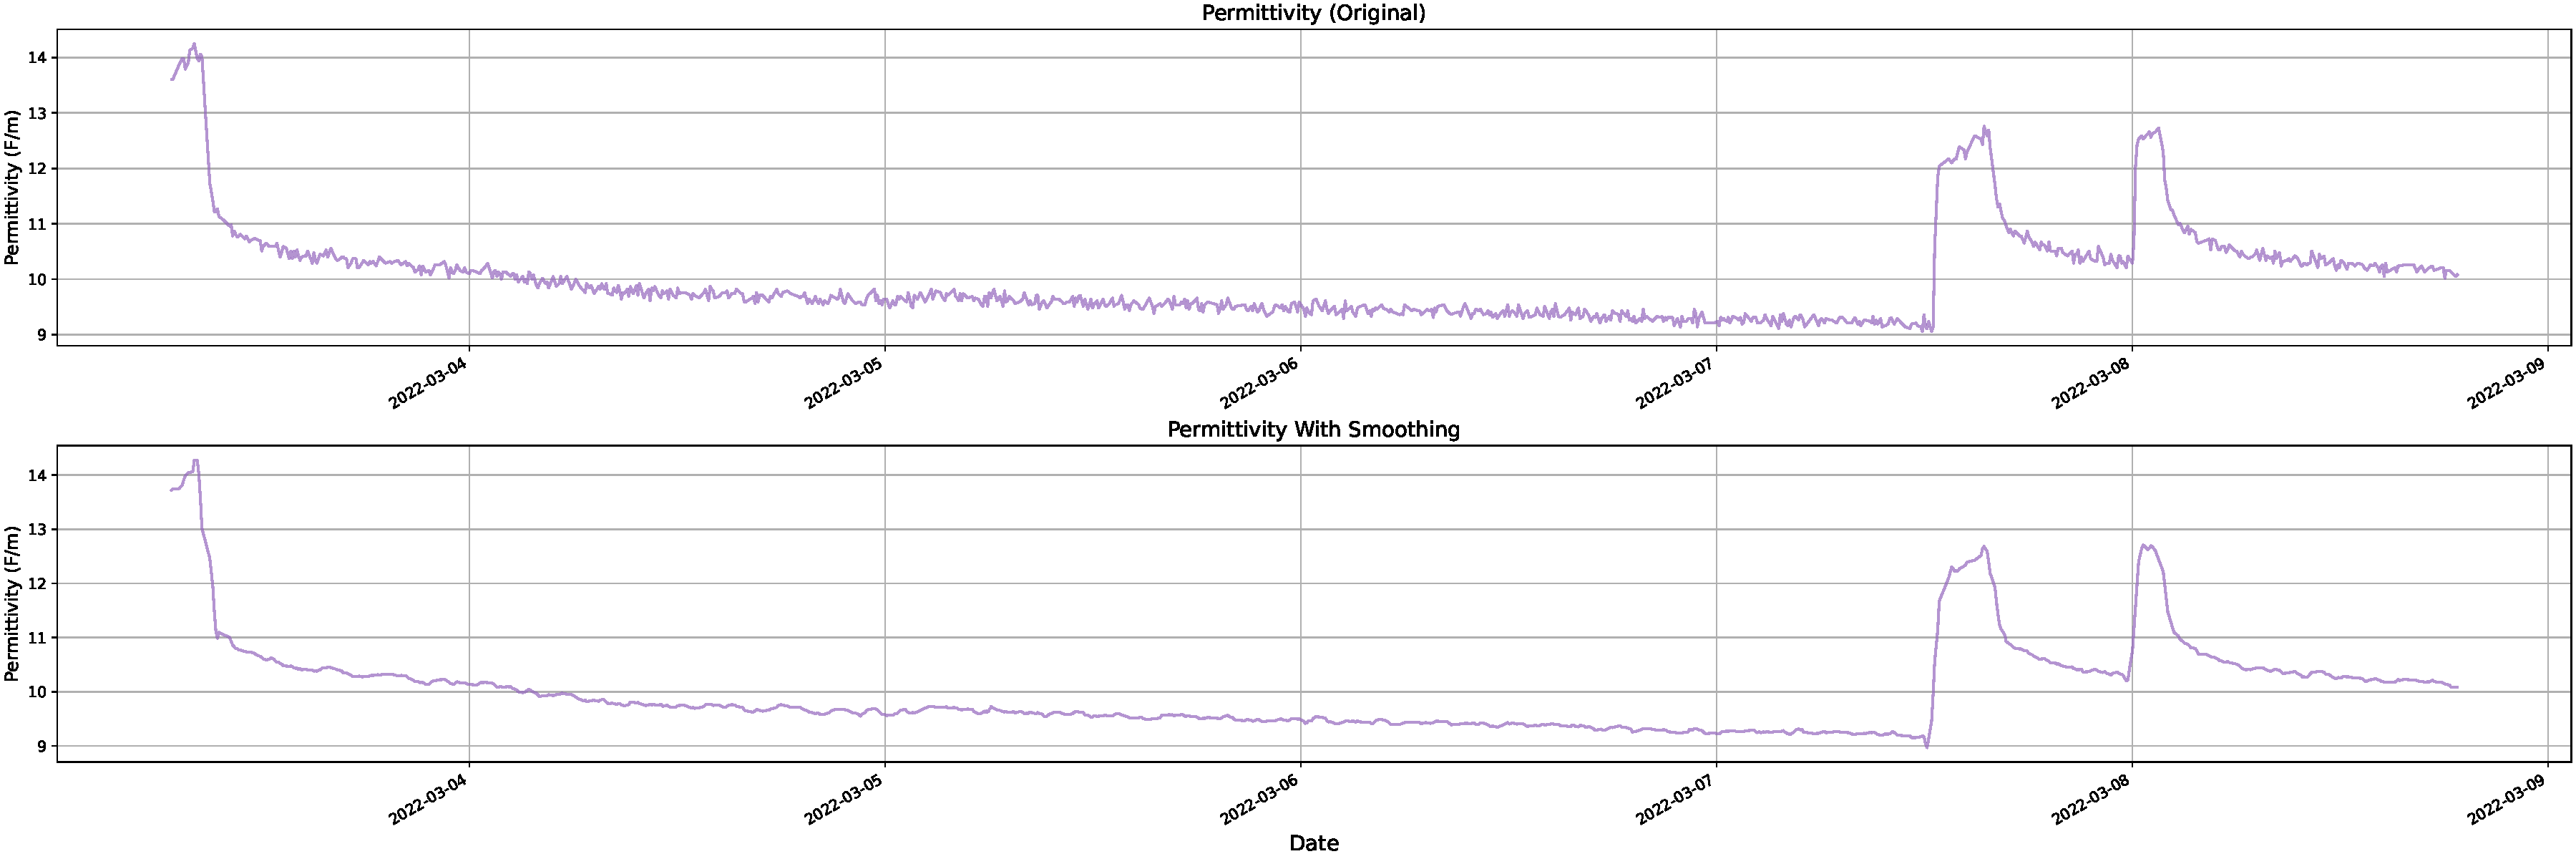
\includegraphics[width=15 cm]{5_ChapterDesign/figuras/2_Smoothing/Smoothing_Permittivity}
    \caption{Original Permittivity data (top) versus the Permittivity smoothed data (bottom) after applying a Savitzky-Golay filter}
    \LABFIG{FIG}
\end{figure}

\begin{figure}[htbp]
    \centering
    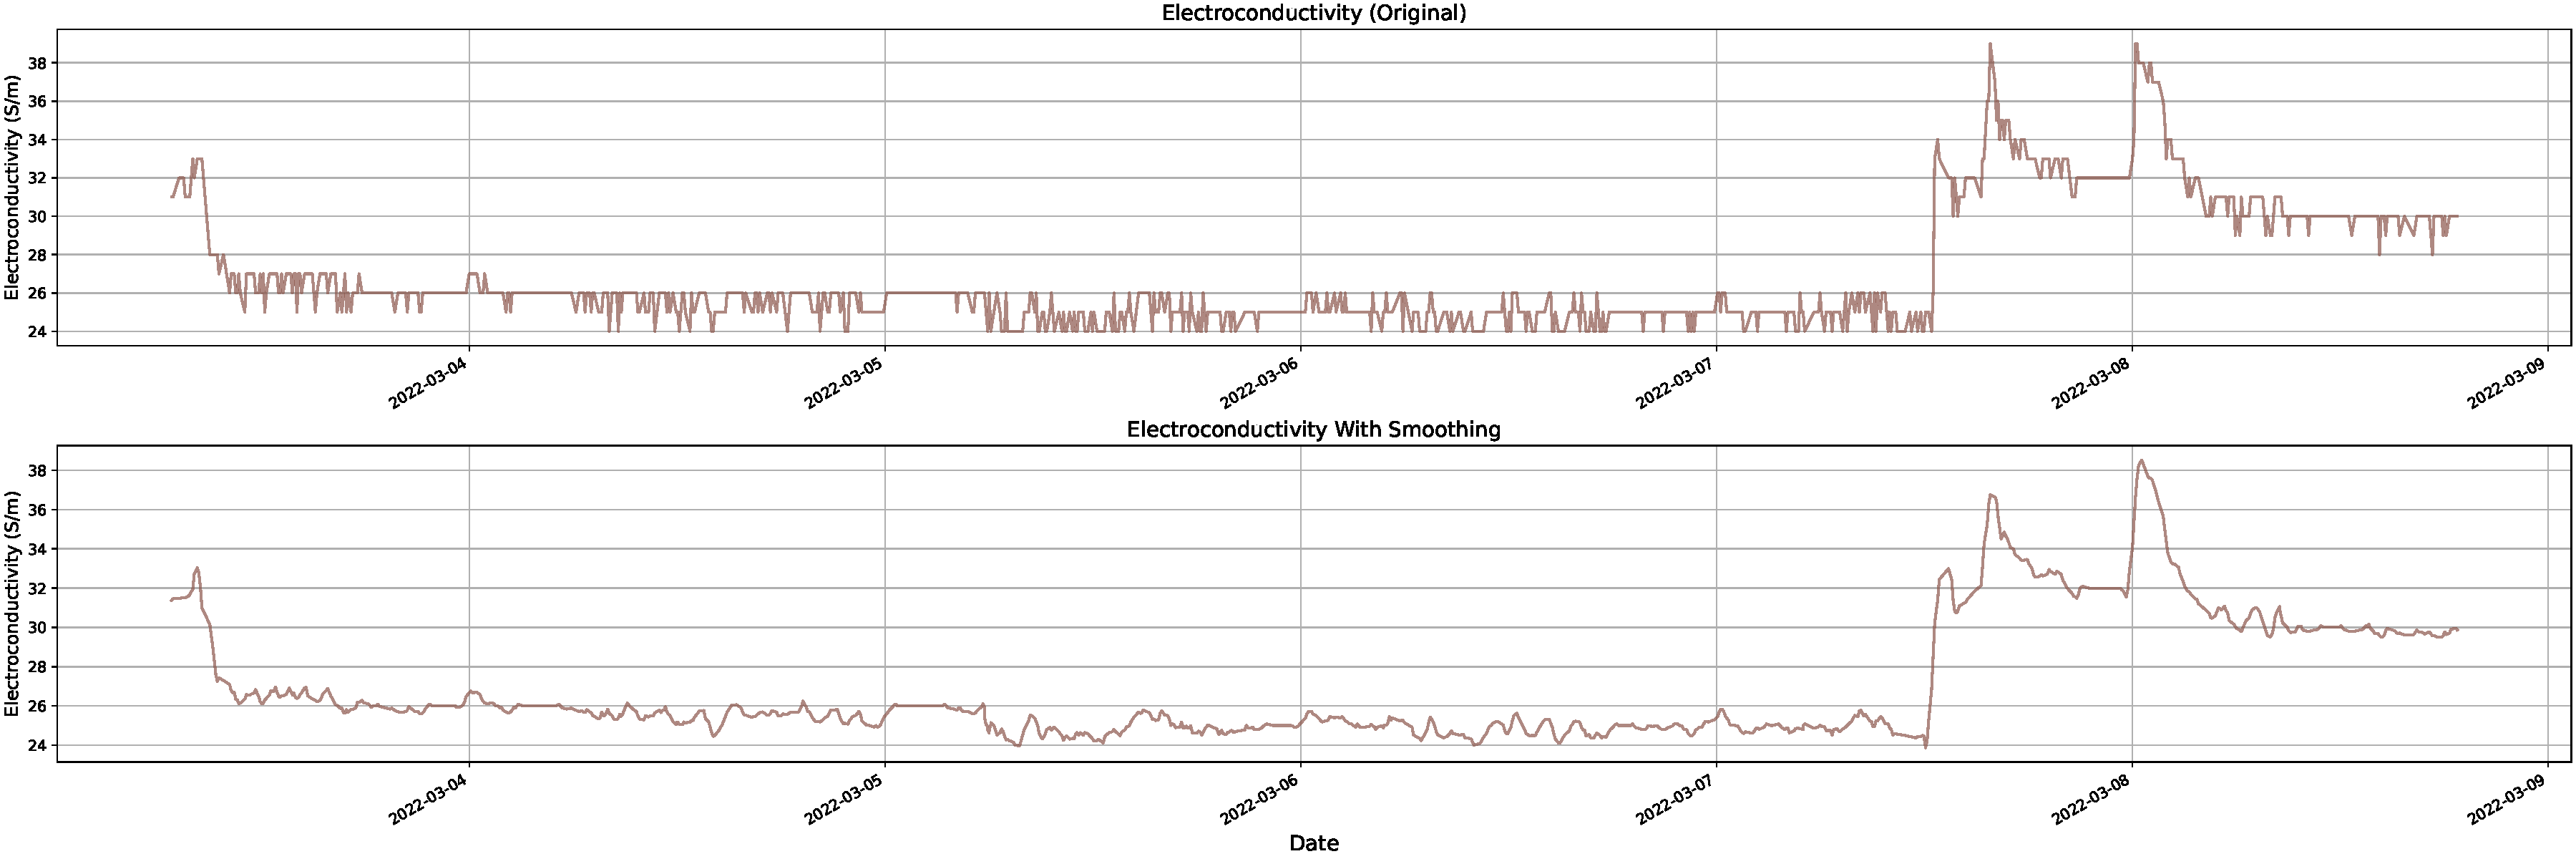
\includegraphics[width=15 cm]{5_ChapterDesign/figuras/2_Smoothing/Smoothing_Electroconductivity}
    \caption{Original Electroconductivity data (top) versus the Electroconductivity smoothed data (bottom) after applying a Savitzky-Golay filter}
    \LABFIG{FIG}
\end{figure}

\begin{figure}[htbp]
    \centering
    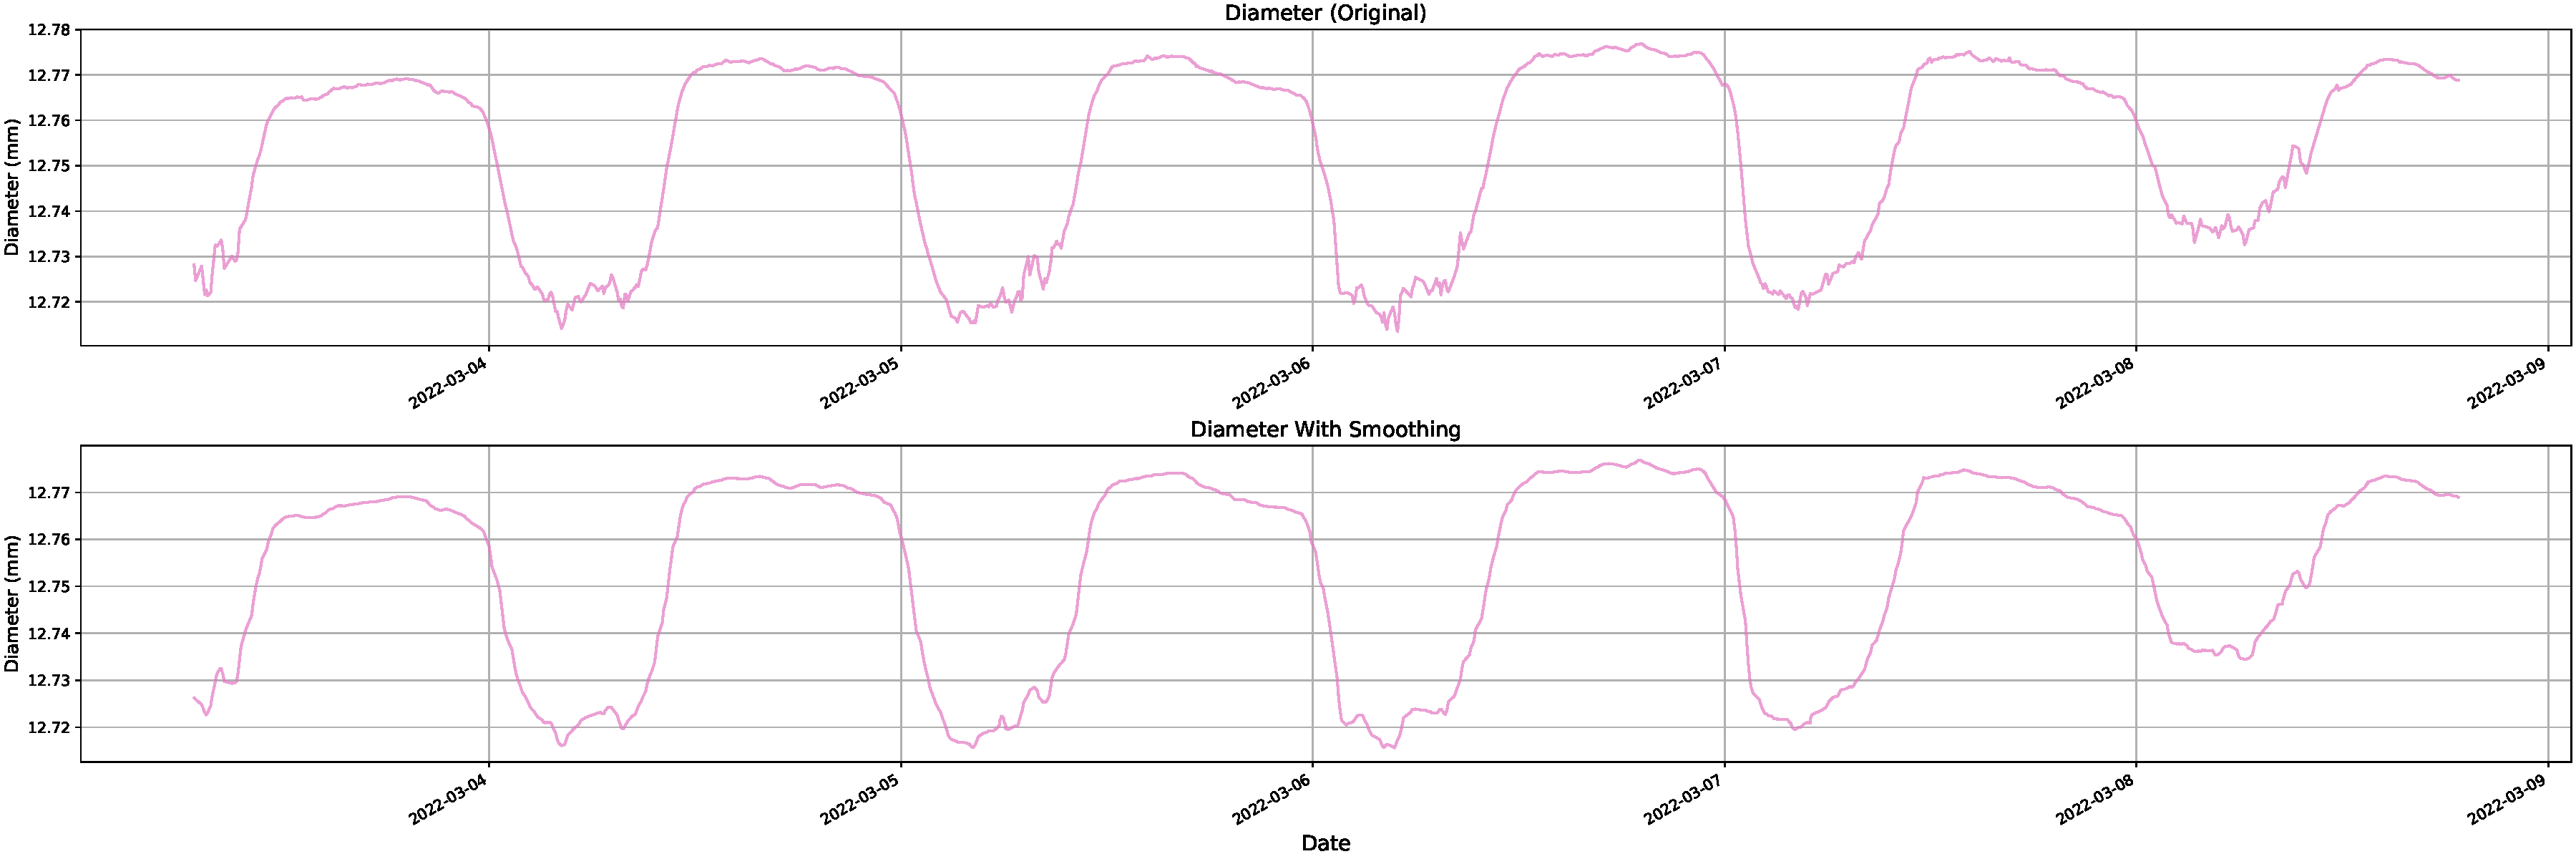
\includegraphics[width=15 cm]{5_ChapterDesign/figuras/2_Smoothing/Smoothing_Diameter}
    \caption{Original Diameter data (top) versus the Diameter smoothed data (bottom) after applying a Savitzky-Golay filter}
    \LABFIG{FIG}
\end{figure}

\begin{figure}[htbp]
    \centering
    
    % Primer par de figuras
    \begin{minipage}[b]{0.45\textwidth}
        \centering
        \begin{subfigure}{\textwidth}
            \centering
            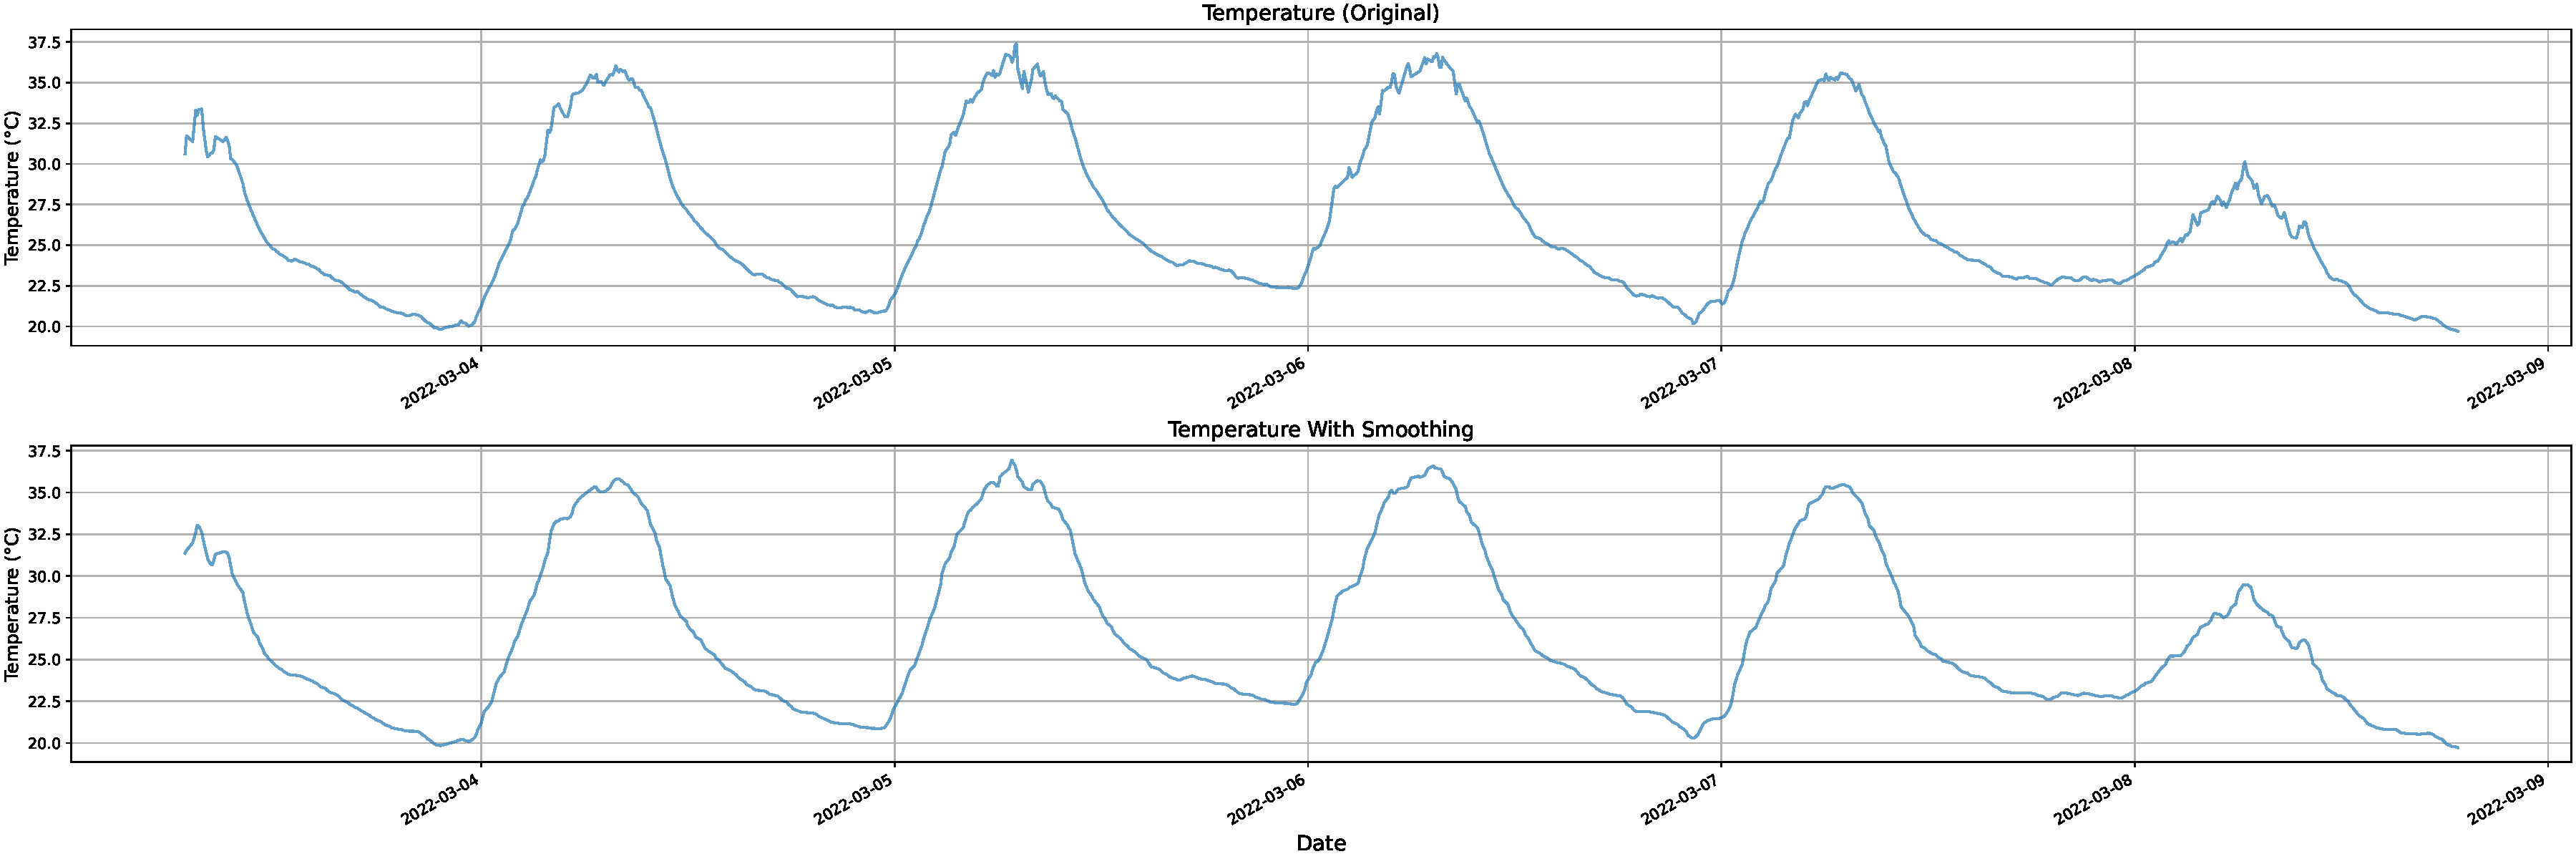
\includegraphics[width=\textwidth]{5_ChapterDesign/figuras/2_Smoothing/Smoothing_Temperature}
            \caption{Original Temperature data (top) versus the Temperature smoothed data (bottom)}
            \label{fig:temperature}
        \end{subfigure}
    \end{minipage}
    \hfill
    \begin{minipage}[b]{0.45\textwidth}
        \centering
        \begin{subfigure}{\textwidth}
            \centering
            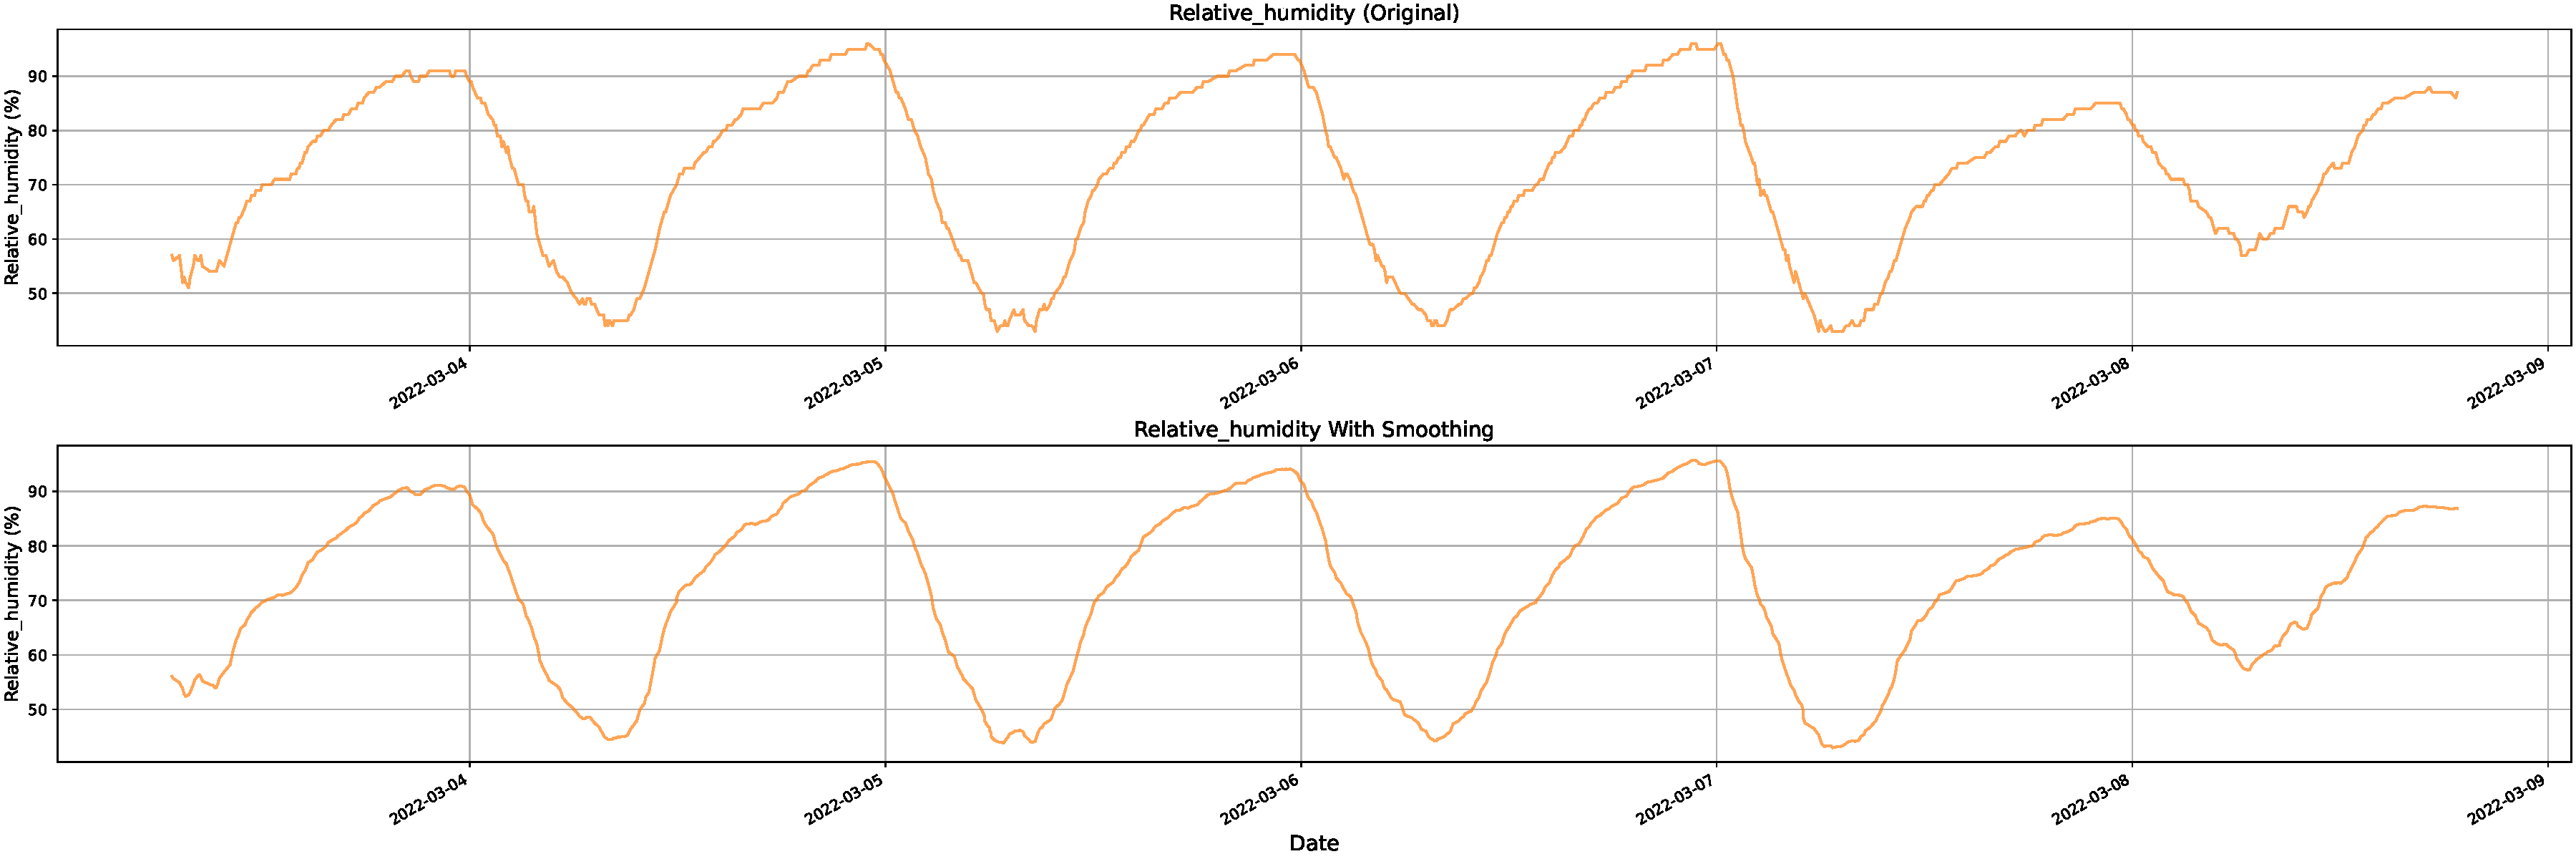
\includegraphics[width=\textwidth]{5_ChapterDesign/figuras/2_Smoothing/Smoothing_Relative_humidity}
            \caption{Original Relative humidity data (top) versus the Relative humidity smoothed data (bottom)}
            \label{fig:relative_humidity}
        \end{subfigure}
    \end{minipage}
    
    \vspace{1em}  % Espacio vertical entre las filas

    % Segundo par de figuras
    \begin{minipage}[b]{0.45\textwidth}
        \centering
        \begin{subfigure}{\textwidth}
            \centering
            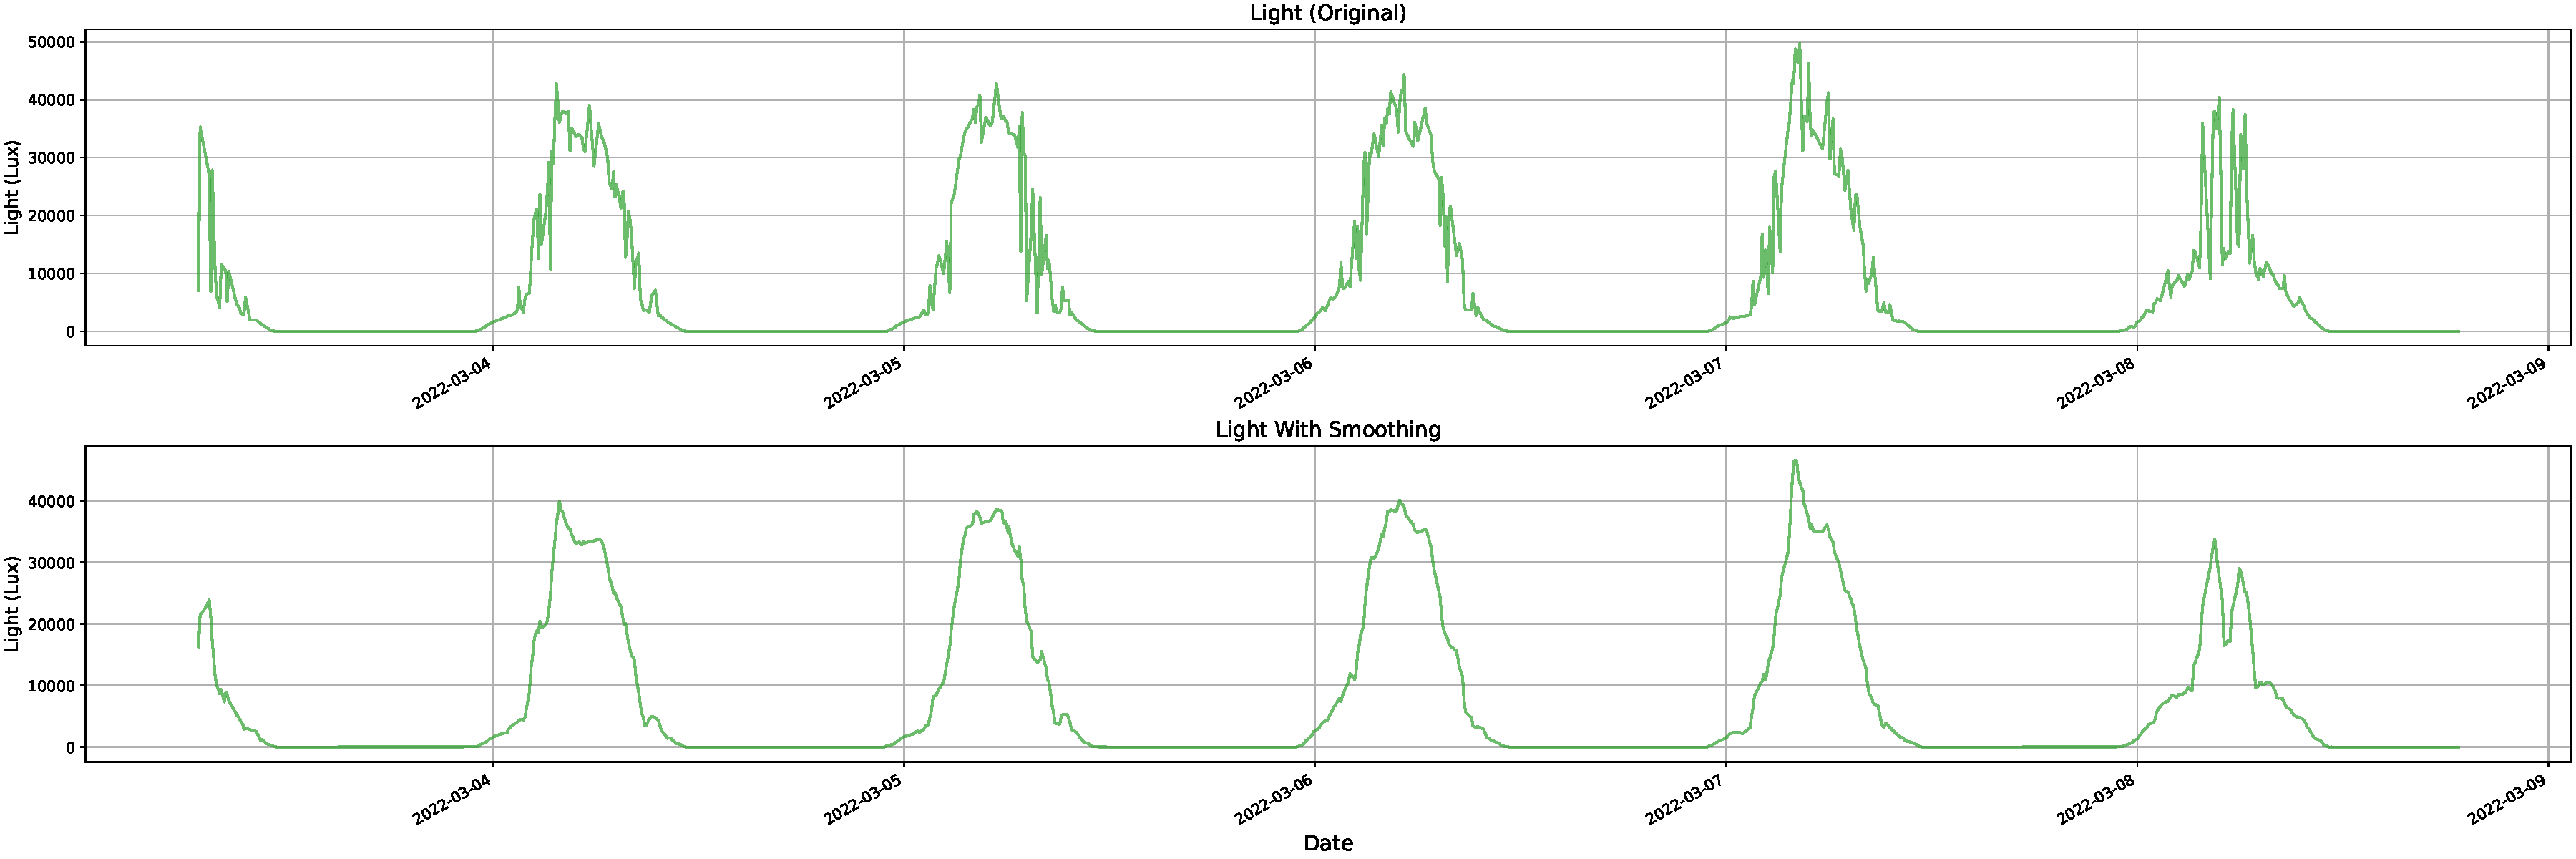
\includegraphics[width=\textwidth]{5_ChapterDesign/figuras/2_Smoothing/Smoothing_Light}
            \caption{Original Light data (top) versus the Light smoothed data (bottom)}
            \label{fig:light}
        \end{subfigure}
    \end{minipage}
    \hfill
    \begin{minipage}[b]{0.45\textwidth}
        \centering
        \begin{subfigure}{\textwidth}
            \centering
            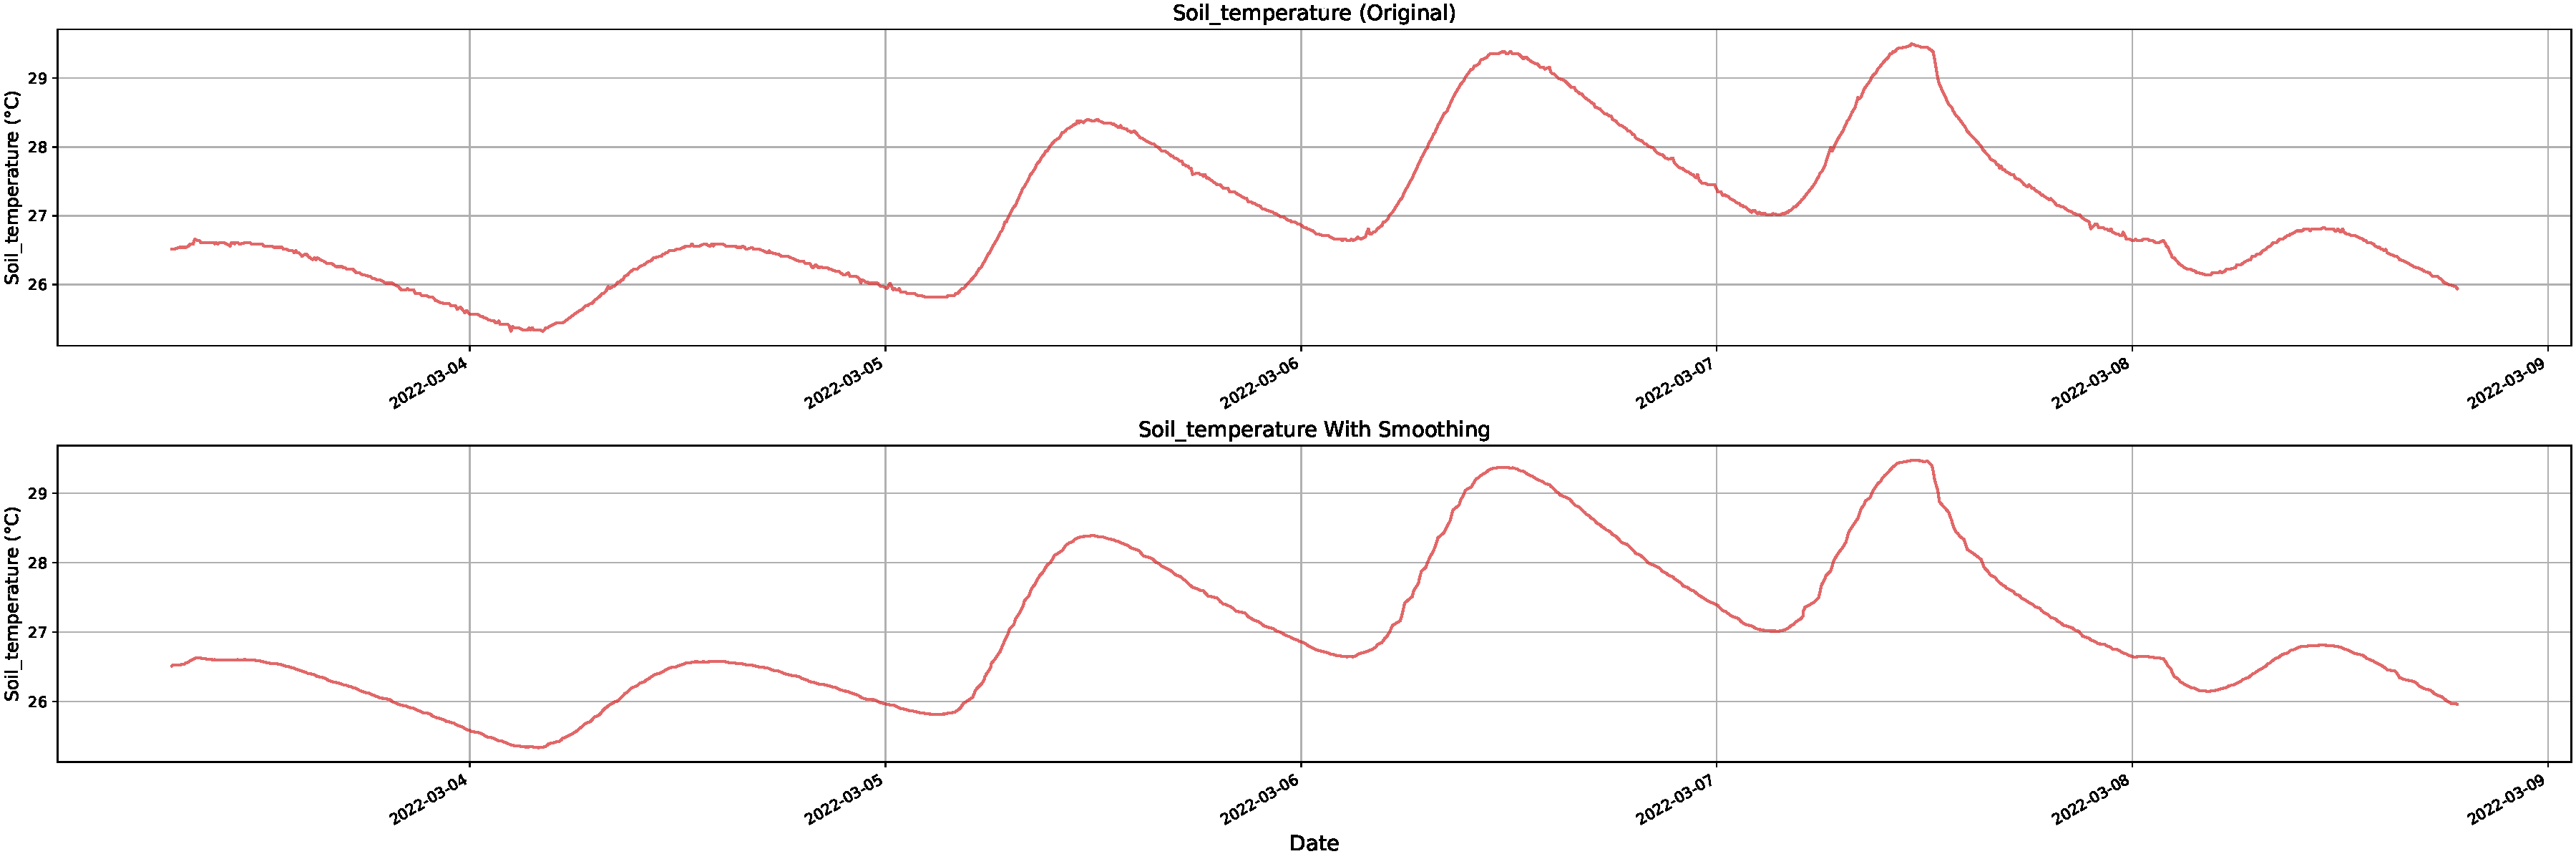
\includegraphics[width=\textwidth]{5_ChapterDesign/figuras/2_Smoothing/Smoothing_Soil_temperature}
            \caption{Original Soil temperature data (top) versus the Soil temperature smoothed data (bottom)}
            \label{fig:soil_temperature}
        \end{subfigure}
    \end{minipage}
    
    \vspace{1em}  % Espacio vertical entre las filas

    % Tercer par de figuras
    \begin{minipage}[b]{0.45\textwidth}
        \centering
        \begin{subfigure}{\textwidth}
            \centering
            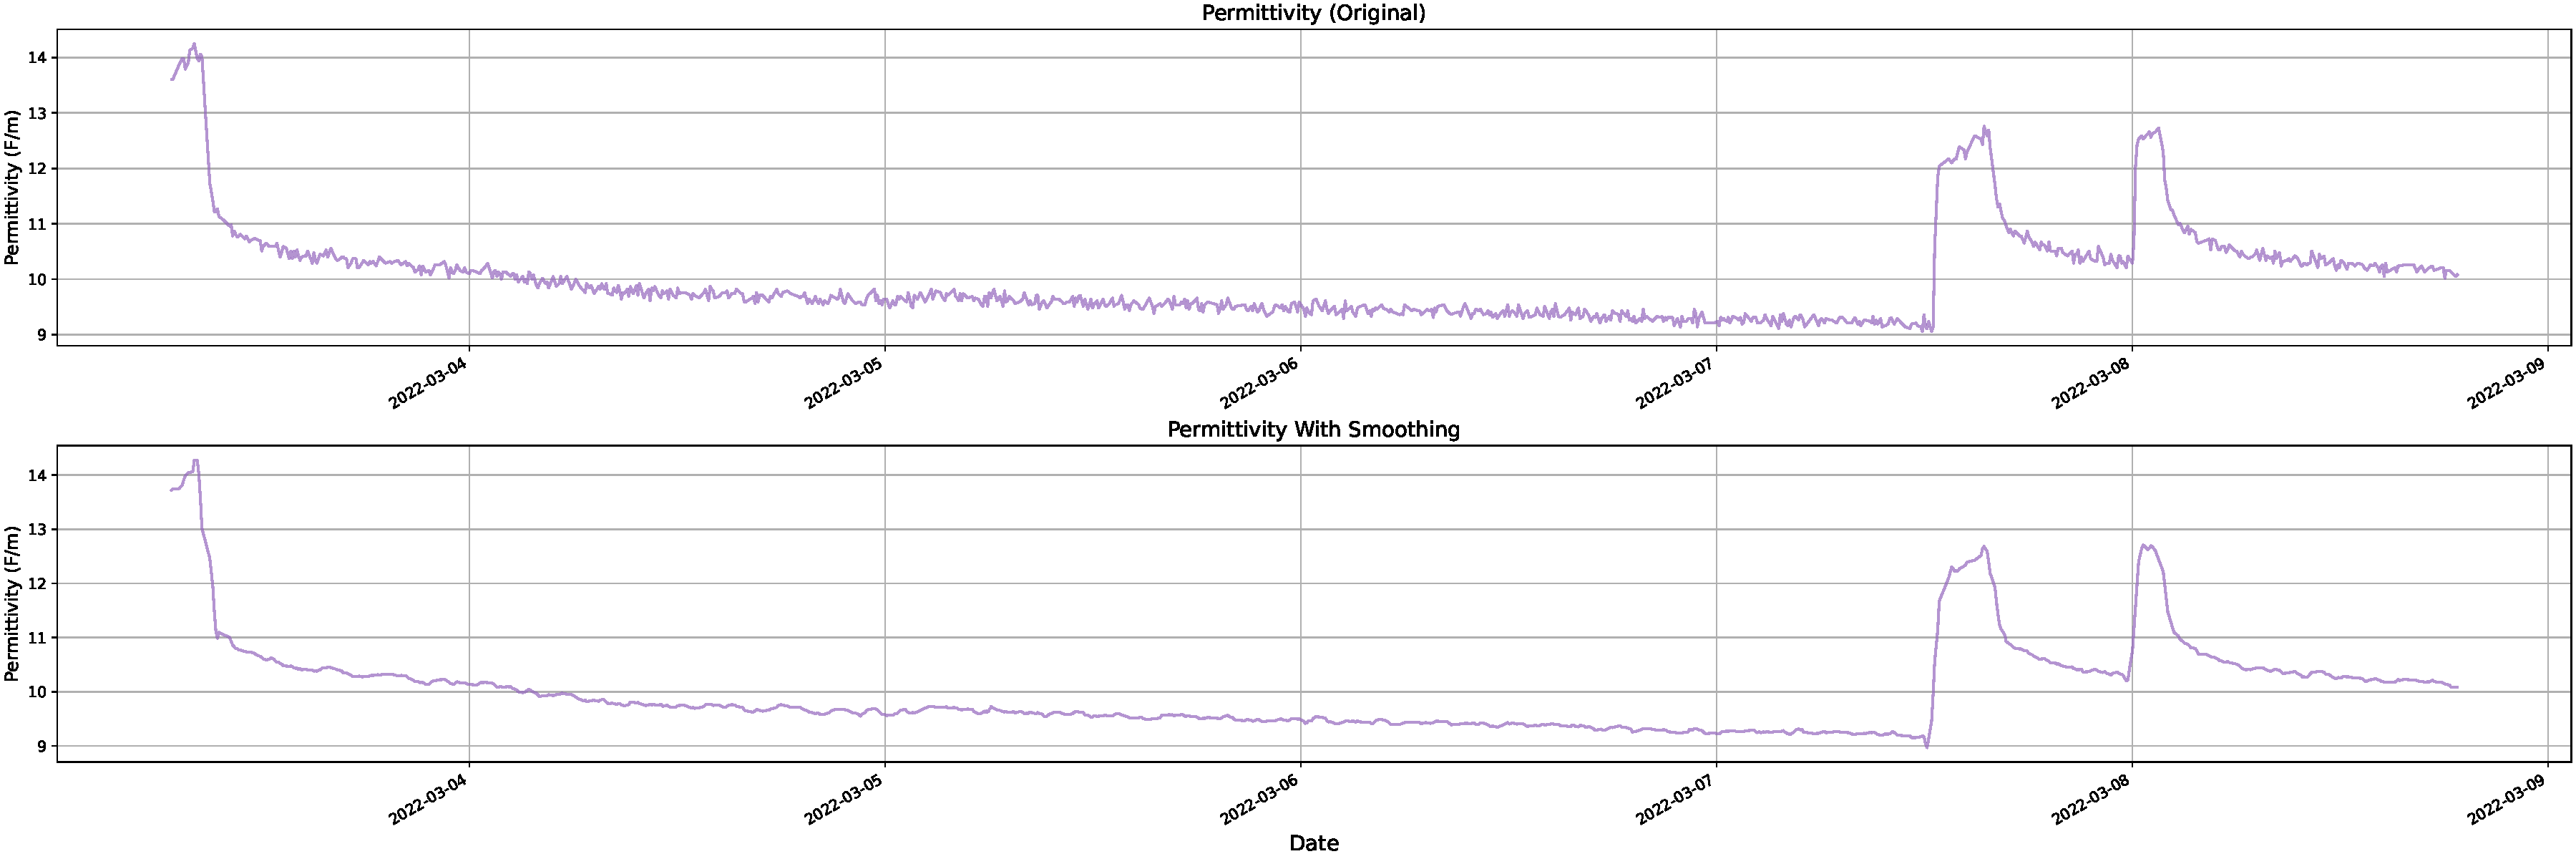
\includegraphics[width=\textwidth]{5_ChapterDesign/figuras/2_Smoothing/Smoothing_Permittivity}
            \caption{Original Permittivity data (top) versus the Permittivity smoothed data (bottom)}
            \label{fig:permittivity}
        \end{subfigure}
    \end{minipage}
    \hfill
    \begin{minipage}[b]{0.45\textwidth}
        \centering
        \begin{subfigure}{\textwidth}
            \centering
            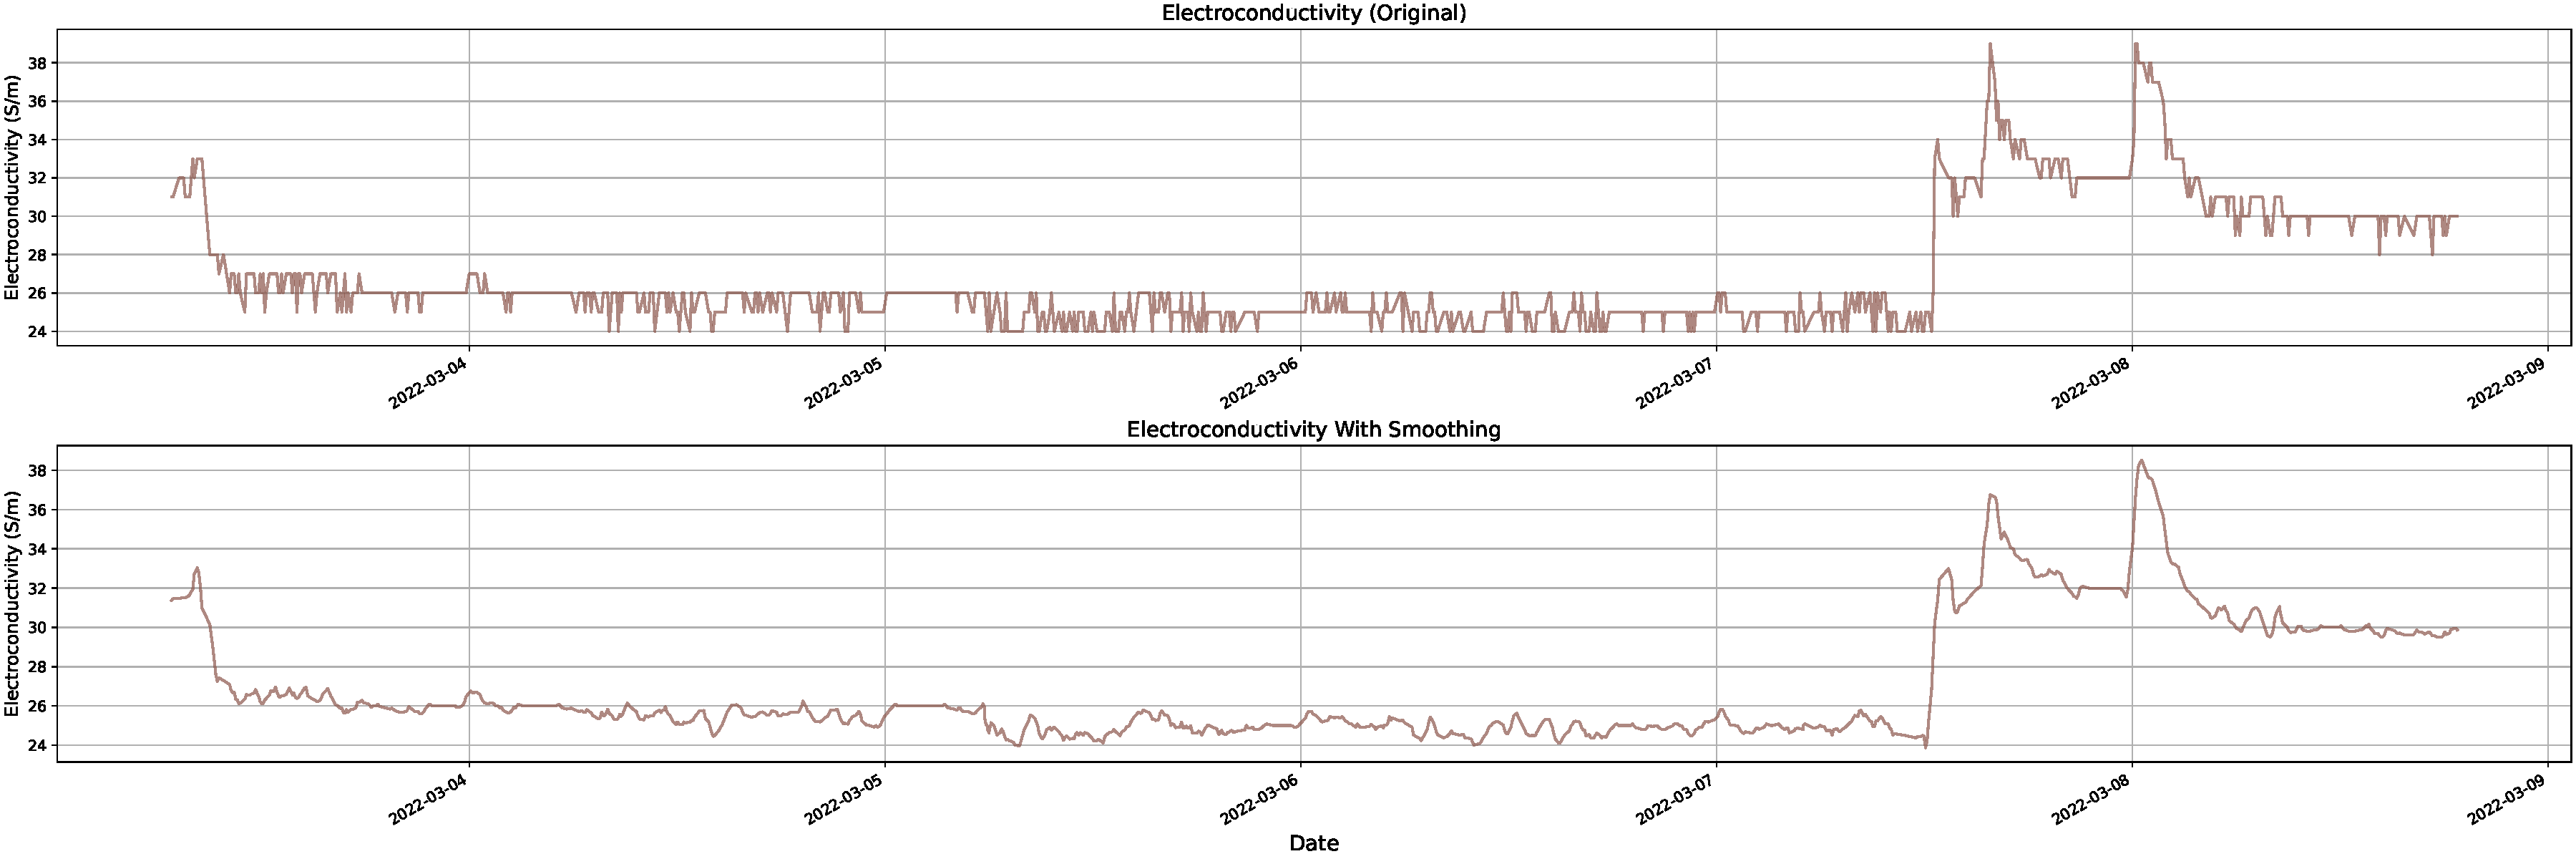
\includegraphics[width=\textwidth]{5_ChapterDesign/figuras/2_Smoothing/Smoothing_Electroconductivity}
            \caption{Original Electroconductivity data (top) versus the Electroconductivity smoothed data (bottom)}
            \label{fig:electroconductivity}
        \end{subfigure}
    \end{minipage}
\end{figure}

This type of smoothing is commonly used in signal processing to reduce noise in datasets and facilitate the identification of patterns and trends. By decreasing background noise, trends emerge more clearly, which is crucial for accurate analysis.


\chapter{Experimental Results}\LABCHAP{CAP6}
\pagestyle{esitscCD}

In this chapter, we present the experimental results obtained from the application of the different hyperparameter configurations for our models. The results are summarized in a series of tables, detailing the R-squared (R²), Mean Squared Error (MSE), and training time for each stage of the experimental development. These metrics provide a comprehensive comparison of the models' effectiveness and efficiency across different configurations.

\section{Results Changing the Prediction Length and Context Length}
This section presents the results obtained by varying the Prediction Length and Context Length parameters. These experiments aim to assess how different input and output sequence lengths impact the performance of the models.
In this initial phase, we do not select the best model solely based on error metrics; instead, we also consider the practical utility of the predicted information. For instance, while some early models achieved favorable error indices, predicting only half a day into the future is not practically useful for our purposes (we require predictions that extend several days ahead). Consequently, in this phase, we chose Models T3, I3, and A3 as the best options, as they provide the most useful predictions in practice, despite not having the lowest error indices.

\subsection{Transformer}
The results for the Transformer variant, as shown in Tables \ref{T1_M} and \ref{T1_R}, indicate that models T4, T7, and T8 perform worse than the other models due to working with larger datasets. This decline in performance might be due to the current selection of other hyperparameters, which could be limiting the model's ability to effectively handle increased Prediction Length and Context Length. On the other hand, as previously discussed, while models T1 and T2 achieve good error metrics, their short-term predictions are not practical for our objectives, as we need to predict at least two days into the future, as demonstrated by Model T3.

Additionally, Table \ref{T1_T}, shows that training time increases as the Prediction Length and Context Length grow, illustrating the trade-off between prediction horizon and computational cost.

A comparison between the predictions of the T3 model and the actual values of the 7 variables is illustrated in Figure \ref{T3}. This figure highlights the accuracy of the T3 model over a two-day prediction horizon, providing a clear visual representation of its performance across different variables.


\begin{table}[]
    \centering
    \resizebox{\textwidth}{!}{%
    \begin{tabular}{
    >{\columncolor[HTML]{FFFFFF}}c cccccccc}
    \multicolumn{9}{c}{\cellcolor[HTML]{FFFFFF}\textbf{MSE   (Sorted by model)}}                                                                                                                                                                                                                                                 \\
    Model & \cellcolor[HTML]{FFFFFF}Diameter & \cellcolor[HTML]{FFFFFF}Electroconductivity & \cellcolor[HTML]{FFFFFF}Light  & \cellcolor[HTML]{FFFFFF}Permittivity & \cellcolor[HTML]{FFFFFF}Relative Humidity & \cellcolor[HTML]{FFFFFF}Soil Temperature & \cellcolor[HTML]{FFFFFF}Temperature & \cellcolor[HTML]{FFFFFF}Mean   \\
    T1    & \cellcolor[HTML]{63BE7B}-21.03   & \cellcolor[HTML]{FFD981}-36.01              & \cellcolor[HTML]{E0E282}-15.53 & \cellcolor[HTML]{E5E382}-27.48       & \cellcolor[HTML]{63BE7B}-20.93            & \cellcolor[HTML]{DAE081}-20.54           & \cellcolor[HTML]{63BE7B}-22.36      & \cellcolor[HTML]{A3D07E}-23.41 \\
    T2    & \cellcolor[HTML]{90CB7D}-20.41   & \cellcolor[HTML]{92CB7D}-41.05              & \cellcolor[HTML]{63BE7B}-24.16 & \cellcolor[HTML]{6FC17B}-30.03       & \cellcolor[HTML]{7AC47C}-19.94            & \cellcolor[HTML]{FCEA83}-19.39           & \cellcolor[HTML]{DEE182}-18.66      & \cellcolor[HTML]{63BE7B}-24.80 \\
    T3    & \cellcolor[HTML]{CDDC81}-19.57   & \cellcolor[HTML]{63BE7B}-42.84              & \cellcolor[HTML]{FFEA84}-13.43 & \cellcolor[HTML]{F8696B}-22.45       & \cellcolor[HTML]{FBEA83}-14.39            & \cellcolor[HTML]{63BE7B}-24.66           & \cellcolor[HTML]{CCDC81}-19.19      & \cellcolor[HTML]{D5DE81}-22.36 \\
    T4    & \cellcolor[HTML]{FDBD7C}-17.29   & \cellcolor[HTML]{F8696B}-30.49              & \cellcolor[HTML]{FCB279}-12.61 & \cellcolor[HTML]{F97A6F}-23.01       & \cellcolor[HTML]{F8696B}-9.84             & \cellcolor[HTML]{F8696B}-10.60           & \cellcolor[HTML]{FB9975}-14.61      & \cellcolor[HTML]{F8696B}-16.92 \\
    T5    & \cellcolor[HTML]{FDBD7B}-17.29   & \cellcolor[HTML]{FFEB84}-36.85              & \cellcolor[HTML]{F8696B}-11.57 & \cellcolor[HTML]{FCAA78}-24.69       & \cellcolor[HTML]{FCB079}-12.22            & \cellcolor[HTML]{FCAD79}-15.14           & \cellcolor[HTML]{F96E6C}-13.02      & \cellcolor[HTML]{FB9C75}-18.68 \\
    T6    & \cellcolor[HTML]{6BC07B}-20.91   & \cellcolor[HTML]{83C77C}-41.59              & \cellcolor[HTML]{F1E783}-14.35 & \cellcolor[HTML]{64BE7B}-30.26       & \cellcolor[HTML]{97CD7E}-18.68            & \cellcolor[HTML]{FCB27A}-15.48           & \cellcolor[HTML]{8AC97D}-21.17      & \cellcolor[HTML]{ADD37F}-23.21 \\
    T7    & \cellcolor[HTML]{F8696B}-14.43   & \cellcolor[HTML]{FDEA83}-36.95              & \cellcolor[HTML]{F96D6C}-11.62 & \cellcolor[HTML]{FFDC81}-26.39       & \cellcolor[HTML]{FA7D6F}-10.51            & \cellcolor[HTML]{C5DA80}-21.29           & \cellcolor[HTML]{F8696B}-12.84      & \cellcolor[HTML]{FCA978}-19.15 \\
    T8    & \cellcolor[HTML]{FED881}-18.22   & \cellcolor[HTML]{FA8871}-31.98              & \cellcolor[HTML]{FEEA83}-13.46 & \cellcolor[HTML]{63BE7B}-30.30       & \cellcolor[HTML]{FFE784}-14.11            & \cellcolor[HTML]{FFEA84}-19.20           & \cellcolor[HTML]{FED17F}-16.70      & \cellcolor[HTML]{FED280}-20.57
    \end{tabular}%
    }
    \caption{Mean Squared Errors (MSE) for different Transformer models obtained by varying the prediction length and context length, sorted by model}
    \label{T1_M}
    \end{table}


\begin{table}[]
    \centering
    \resizebox{\textwidth}{!}{%
    \begin{tabular}{
    >{\columncolor[HTML]{FFFFFF}}c cccccccc}
    \multicolumn{9}{c}{\cellcolor[HTML]{FFFFFF}\textbf{R2 (Sorted by model)}}                                                                                                                                                                                                                                                         \\
    Model & \cellcolor[HTML]{FFFFFF}Diameter & \cellcolor[HTML]{FFFFFF}Electroconductivity & \cellcolor[HTML]{FFFFFF}Light    & \cellcolor[HTML]{FFFFFF}Permittivity & \cellcolor[HTML]{FFFFFF}Relative\_humidity & \cellcolor[HTML]{FFFFFF}Soil\_Temperature & \cellcolor[HTML]{FFFFFF}Temperature & \cellcolor[HTML]{FFFFFF}Mean    \\
    T1    & \cellcolor[HTML]{63BE7B}0.64     & \cellcolor[HTML]{FDD47F}-3.07               & \cellcolor[HTML]{63BE7B}0.48     & \cellcolor[HTML]{FBA376}-9.84        & \cellcolor[HTML]{63BE7B}0.85               & \cellcolor[HTML]{C0D981}-1.77             & \cellcolor[HTML]{63BE7B}0.85        & \cellcolor[HTML]{FEEA83}-1.69   \\
    T2    & \cellcolor[HTML]{FA9874}-0.28    & \cellcolor[HTML]{FDCE7E}-3.28               & \cellcolor[HTML]{F8696B}-1392.03 & \cellcolor[HTML]{F8696B}-13.68       & \cellcolor[HTML]{F86C6B}-1.04              & \cellcolor[HTML]{FEE482}-3.85             & \cellcolor[HTML]{F8696B}-7.68       & \cellcolor[HTML]{F8696B}-203.12 \\
    T3    & \cellcolor[HTML]{AAD380}0.50     & \cellcolor[HTML]{63BE7B}0.36                & \cellcolor[HTML]{CCDD82}0.21     & \cellcolor[HTML]{F98B71}-11.43       & \cellcolor[HTML]{CFDD82}0.28               & \cellcolor[HTML]{63BE7B}0.09              & \cellcolor[HTML]{91CC7E}0.69        & \cellcolor[HTML]{DCE182}-1.33   \\
    T4    & \cellcolor[HTML]{F9EA84}0.35     & \cellcolor[HTML]{FA8F72}-5.48               & \cellcolor[HTML]{FEEA83}-0.07    & \cellcolor[HTML]{AED480}-3.04        & \cellcolor[HTML]{F8696B}-1.08              & \cellcolor[HTML]{F8696B}-20.05            & \cellcolor[HTML]{FEE883}0.17        & \cellcolor[HTML]{FEE983}-4.17   \\
    T5    & \cellcolor[HTML]{FDD37F}0.16     & \cellcolor[HTML]{D3DF82}-1.54               & \cellcolor[HTML]{FEEA83}-0.22    & \cellcolor[HTML]{FED880}-6.42        & \cellcolor[HTML]{FDD27F}-0.19              & \cellcolor[HTML]{FDCB7D}-7.14             & \cellcolor[HTML]{FEE182}-0.27       & \cellcolor[HTML]{FEEA83}-2.23   \\
    T6    & \cellcolor[HTML]{67BF7C}0.63     & \cellcolor[HTML]{70C27C}0.15                & \cellcolor[HTML]{93CC7E}0.36     & \cellcolor[HTML]{64BF7C}-1.06        & \cellcolor[HTML]{79C57D}0.73               & \cellcolor[HTML]{FDD07E}-6.53             & \cellcolor[HTML]{71C27C}0.81        & \cellcolor[HTML]{63BE7B}-0.70   \\
    T7    & \cellcolor[HTML]{F8696B}-0.63    & \cellcolor[HTML]{D0DE82}-1.49               & \cellcolor[HTML]{FEEA83}-0.20    & \cellcolor[HTML]{D3DF82}-4.02        & \cellcolor[HTML]{FA8E72}-0.76              & \cellcolor[HTML]{99CE7F}-0.98             & \cellcolor[HTML]{FEE081}-0.33       & \cellcolor[HTML]{C3DA81}-1.20   \\
    T8    & \cellcolor[HTML]{FEE983}0.32     & \cellcolor[HTML]{F8696B}-6.80               & \cellcolor[HTML]{C9DC81}0.21     & \cellcolor[HTML]{63BE7B}-1.04        & \cellcolor[HTML]{D8E082}0.23               & \cellcolor[HTML]{D6E082}-2.20             & \cellcolor[HTML]{D6E082}0.46        & \cellcolor[HTML]{CFDE82}-1.26  
    \end{tabular}%
    }
    \caption{R-squared (R²) for different Transformer models obtained by varying the prediction length and context length, sorted by model}
    \label{T1_R}
    \end{table}

\begin{table}[]
    \begin{tabular}{
    >{\columncolor[HTML]{FFFFFF}}c cc
    >{\columncolor[HTML]{FFFFFF}}c c}
    \multicolumn{2}{c}{\cellcolor[HTML]{FFFFFF}\textbf{Training   Time (Sorted by model)}} & \cellcolor[HTML]{FFFFFF} & \multicolumn{2}{c}{\cellcolor[HTML]{FFFFFF}\textbf{Training Time (Sorted   by training time)}} \\
    Model                  & \cellcolor[HTML]{FFFFFF}Training time {[}s{]}                 & \cellcolor[HTML]{FFFFFF} & Model                      & \cellcolor[HTML]{FFFFFF}Training time {[}s{]}                     \\
    T1                     & \cellcolor[HTML]{76C37C}98.82                                 &                          & T2                         & \cellcolor[HTML]{63BE7B}82.07                                     \\
    T2                     & \cellcolor[HTML]{63BE7B}82.07                                 &                          & T1                         & \cellcolor[HTML]{76C37C}98.82                                     \\
    T3                     & \cellcolor[HTML]{FFDD82}249.05                                &                          & T5                         & \cellcolor[HTML]{A1D07E}137.13                                    \\
    T4                     & \cellcolor[HTML]{F8696B}495.8                                 &                          & T6                         & \cellcolor[HTML]{DCE081}188.07                                    \\
    T5                     & \cellcolor[HTML]{A1D07E}137.13                                &                          & T3                         & \cellcolor[HTML]{FFDD82}249.05                                    \\
    T6                     & \cellcolor[HTML]{DCE081}188.07                                &                          & T7                         & \cellcolor[HTML]{FDB47A}336.09                                    \\
    T7                     & \cellcolor[HTML]{FDB47A}336.09                                &                          & T8                         & \cellcolor[HTML]{FA8C72}422.95                                    \\
    T8                     & \cellcolor[HTML]{FA8C72}422.95                                &                          & T4                         & \cellcolor[HTML]{F8696B}495.8                                    
    \end{tabular}%
    \caption{Training times for different Transformer models obtained by varying the prediction length and context length, sorted by model and training time values}
    \label{T1_T}
    \end{table}

\begin{figure}[htbp]
    \centering
    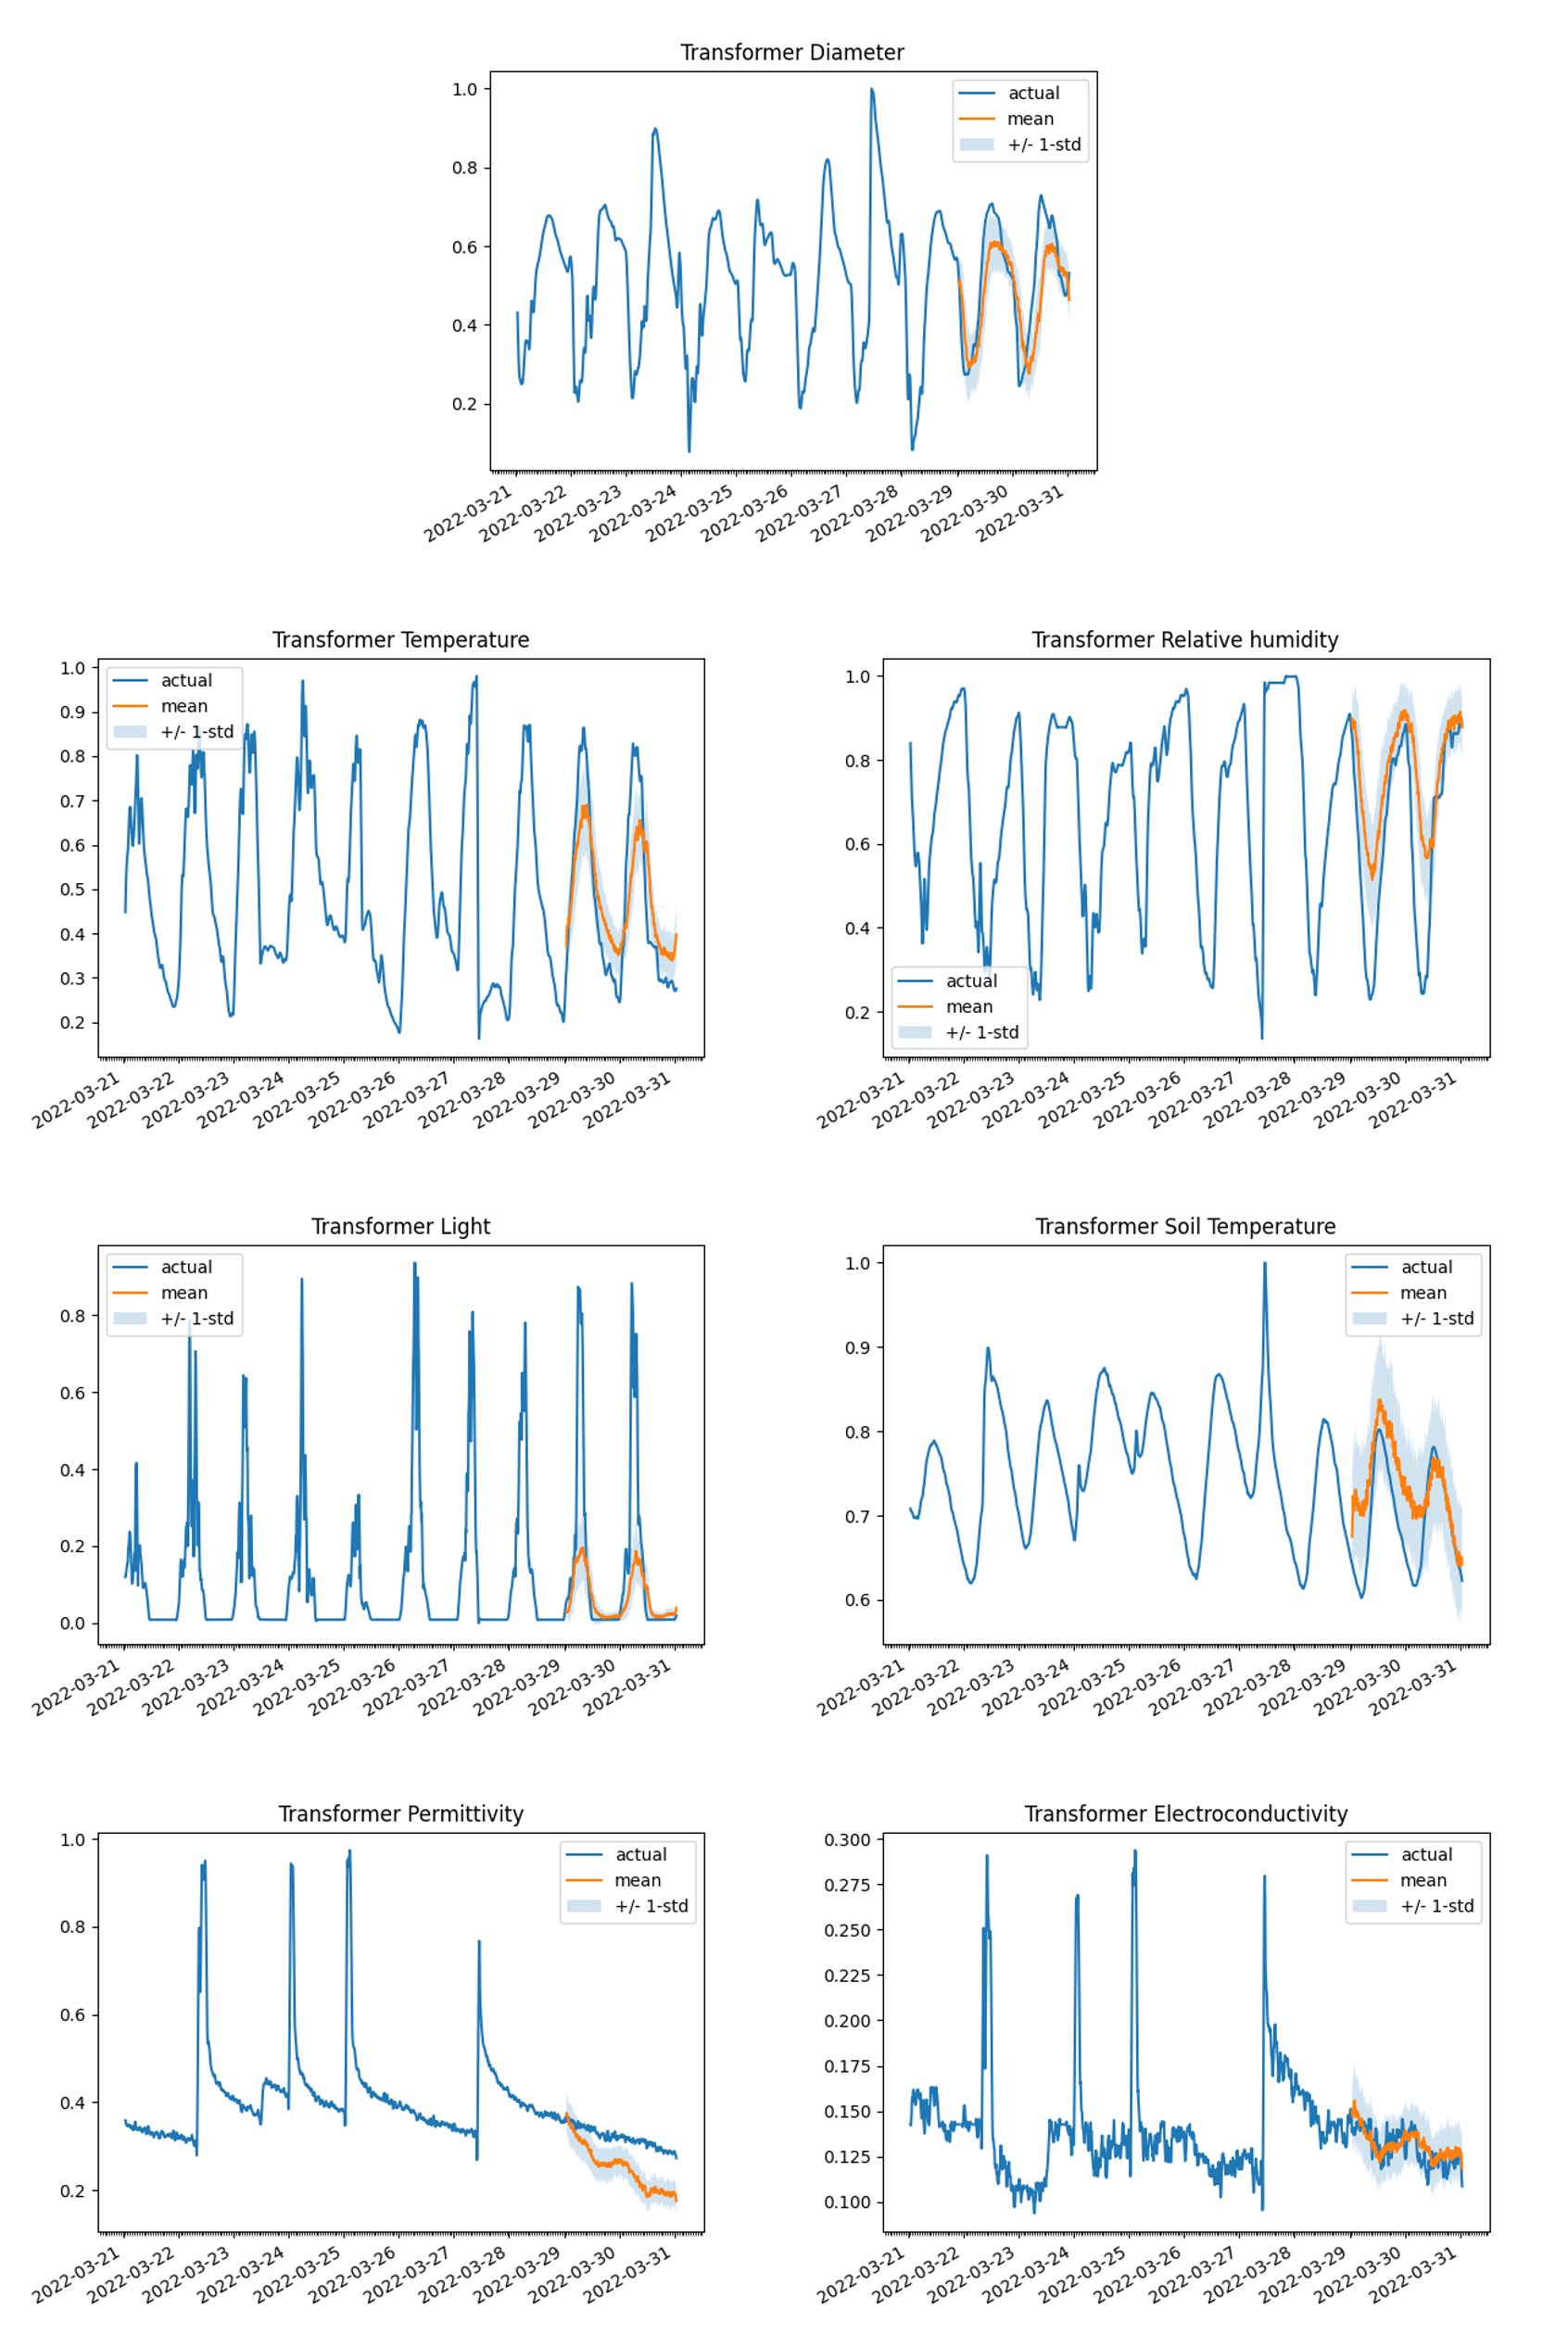
\includegraphics[width=15 cm]{6_ChapterResults/figuras/T3.png}
    \caption{Comparison between the predicted values generated by the T3 model and the actual observed values for the 7 variables over a two-day prediction horizon}
    \label{T3}
\end{figure}

\subsection{Informer}
The results for the Informer variant, as presented in Tables \ref{I1_M} and \ref{I1_R}, show similarities to those observed with the Transformer. However, unlike the Transformer, the Informer demonstrates a greater capability to handle larger Prediction Length and Context Length values more effectively. This suggests that the Informer is better suited for scenarios requiring longer forecasting horizons.

Additionally, Table \ref{I1_T} reveals a significant reduction in training time for models that work with larger datasets, such as T3, T4, T6, T7, and T8. Conversely, when the amount of data is smaller, as in models T1, T2, and T5, the training time increases. This highlights the Informer's efficiency in dealing with larger data volumes, while it may require more time when working with smaller datasets.

Figure \ref{I3} presents a comparison between the I3 model's predictions and the actual values of the 7 variables. This illustration emphasizes the I3 model's accuracy over a two-day prediction horizon, offering a clear visual insight into its performance across the variables.

\begin{table}[ht]
    \centering
    \resizebox{\textwidth}{!}{%
    \begin{tabular}{ccccccccc}
    \rowcolor[HTML]{FFFFFF} 
    \multicolumn{9}{c}{\cellcolor[HTML]{FFFFFF}\textbf{MSE   (Sorted by model)}} \\
    \rowcolor[HTML]{FFFFFF} 
    Model                      & Diameter                       & Electroconductivity            & Light                          & Permittivity                   & Relative\_humidity             & Soil\_Temperature              & Temperature                    & Mean                           \\
    \cellcolor[HTML]{FFFFFF}I1 & \cellcolor[HTML]{FA8070}-13.37 & \cellcolor[HTML]{63BE7B}-41.54 & \cellcolor[HTML]{FFE383}-11.66 & \cellcolor[HTML]{63BE7B}-34.17 & \cellcolor[HTML]{FDEA83}-11.18 & \cellcolor[HTML]{C0D880}-17.29 & \cellcolor[HTML]{FBEA83}-11.76 & \cellcolor[HTML]{DBE081}-20.14 \\
    \rowcolor[HTML]{63BE7B} 
    \cellcolor[HTML]{FFFFFF}I2 & -19.28                         & \cellcolor[HTML]{F5E883}-37.85 & -48.90                         & \cellcolor[HTML]{A7D17E}-30.25 & -27.19                         & -25.58                         & -18.46                         & -29.64                         \\
    \cellcolor[HTML]{FFFFFF}I3 & \cellcolor[HTML]{FFDF82}-14.42 & \cellcolor[HTML]{F8696B}-25.45 & \cellcolor[HTML]{FEEA83}-11.71 & \cellcolor[HTML]{F8696B}-17.95 & \cellcolor[HTML]{FAE983}-11.46 & \cellcolor[HTML]{E8E482}-13.71 & \cellcolor[HTML]{E0E282}-12.98 & \cellcolor[HTML]{F96D6C}-15.38 \\
    \cellcolor[HTML]{FFFFFF}I4 & \cellcolor[HTML]{FFDA81}-14.36 & \cellcolor[HTML]{FFDD82}-36.29 & \cellcolor[HTML]{FEEA83}-11.92 & \cellcolor[HTML]{E5E382}-26.62 & \cellcolor[HTML]{FFE583}-10.89 & \cellcolor[HTML]{F8696B}-6.04  & \cellcolor[HTML]{FDC37D}-11.00 & \cellcolor[HTML]{FDC57D}-16.73 \\
    \rowcolor[HTML]{F8696B} 
    \cellcolor[HTML]{FFFFFF}I5 & -13.12                         & \cellcolor[HTML]{FCAE79}-31.83 & -11.34                         & \cellcolor[HTML]{FED280}-23.74 & -7.91                          & \cellcolor[HTML]{FDBF7C}-9.77  & -9.64                          & -15.33                         \\
    \cellcolor[HTML]{FFFFFF}I6 & \cellcolor[HTML]{DAE081}-15.67 & \cellcolor[HTML]{FFE984}-37.37 & \cellcolor[HTML]{FECB7E}-11.60 & \cellcolor[HTML]{9ECF7E}-30.75 & \cellcolor[HTML]{FED680}-10.51 & \cellcolor[HTML]{FA8B72}-7.52  & \cellcolor[HTML]{FFE383}-11.49 & \cellcolor[HTML]{F8E983}-17.85 \\
    \cellcolor[HTML]{FFFFFF}I7 & \cellcolor[HTML]{FAE983}-14.69 & \cellcolor[HTML]{9ECF7E}-40.04 & \cellcolor[HTML]{FCA878}-11.51 & \cellcolor[HTML]{FDB57A}-22.17 & \cellcolor[HTML]{FA8070}-8.45  & \cellcolor[HTML]{FDB77A}-9.43  & \cellcolor[HTML]{FED680}-11.30 & \cellcolor[HTML]{FEC97E}-16.80 \\
    \cellcolor[HTML]{FFFFFF}I8 & \cellcolor[HTML]{9CCE7E}-17.53 & \cellcolor[HTML]{71C27B}-41.18 & \cellcolor[HTML]{FDEA83}-12.00 & \cellcolor[HTML]{FA8471}-19.44 & \cellcolor[HTML]{FBE983}-11.41 & \cellcolor[HTML]{E5E382}-14.00 & \cellcolor[HTML]{C1D980}-14.32 & \cellcolor[HTML]{EFE683}-18.55 \\
    \end{tabular}%
    }
    \caption{Mean Squared Errors (MSE) for different Informer models obtained by varying the prediction length and context length, sorted by model}
    \label{I1_M}
    \end{table}

\begin{table}[]
    \centering
    \resizebox{\textwidth}{!}{%
    \begin{tabular}{
    >{\columncolor[HTML]{FFFFFF}}c cccccccc}
    \multicolumn{9}{c}{\cellcolor[HTML]{FFFFFF}\textbf{R2 (Sorted by model)}}                                                                                                                                                                                                                                                     \\
    Model & \cellcolor[HTML]{FFFFFF}Diameter & \cellcolor[HTML]{FFFFFF}Electroconductivity & \cellcolor[HTML]{FFFFFF}Light & \cellcolor[HTML]{FFFFFF}Permittivity & \cellcolor[HTML]{FFFFFF}Relative\_humidity & \cellcolor[HTML]{FFFFFF}Soil\_Temperature & \cellcolor[HTML]{FFFFFF}Temperature & \cellcolor[HTML]{FFFFFF}Mean   \\
    I1    & \cellcolor[HTML]{F97D6E}-1.10    & \cellcolor[HTML]{82C77D}-0.14               & \cellcolor[HTML]{FEEA83}-0.26 & \cellcolor[HTML]{6DC17C}-1.32        & \cellcolor[HTML]{F3E884}-0.45              & \cellcolor[HTML]{8BCA7E}-4.85             & \cellcolor[HTML]{E9E583}-0.72       & \cellcolor[HTML]{63BE7B}-1.26  \\
    I2    & \cellcolor[HTML]{FEDB81}-0.66    & \cellcolor[HTML]{FDCF7E}-7.95               & \cellcolor[HTML]{F8696B}-3.67 & \cellcolor[HTML]{FEDC81}-12.95       & \cellcolor[HTML]{63BE7B}0.61               & \cellcolor[HTML]{63BE7B}-0.17             & \cellcolor[HTML]{F8696B}-8.10       & \cellcolor[HTML]{C7DB81}-4.70  \\
    I3    & \cellcolor[HTML]{FEE081}-0.63    & \cellcolor[HTML]{F8696B}-34.12              & \cellcolor[HTML]{B8D780}-0.18 & \cellcolor[HTML]{F8696B}-34.00       & \cellcolor[HTML]{EEE784}-0.41              & \cellcolor[HTML]{B9D780}-10.32            & \cellcolor[HTML]{9ECF7F}-0.29       & \cellcolor[HTML]{F8696B}-11.42 \\
    I4    & \cellcolor[HTML]{C5DB81}-0.29    & \cellcolor[HTML]{D6E082}-0.70               & \cellcolor[HTML]{FEEA83}-0.25 & \cellcolor[HTML]{63BE7B}-0.76        & \cellcolor[HTML]{FEE382}-0.63              & \cellcolor[HTML]{F8696B}-59.17            & \cellcolor[HTML]{FEE983}-0.91       & \cellcolor[HTML]{FBAC77}-8.96  \\
    I5    & \cellcolor[HTML]{F8696B}-1.20    & \cellcolor[HTML]{FDD37F}-7.08               & \cellcolor[HTML]{FEE983}-0.28 & \cellcolor[HTML]{DFE283}-8.24        & \cellcolor[HTML]{F8696B}-2.20              & \cellcolor[HTML]{FDD07E}-27.03            & \cellcolor[HTML]{FEDA80}-1.77       & \cellcolor[HTML]{FEE683}-6.83  \\
    I6    & \cellcolor[HTML]{B8D780}-0.22    & \cellcolor[HTML]{FEE983}-1.26               & \cellcolor[HTML]{D8E082}-0.21 & \cellcolor[HTML]{65BF7C}-0.84        & \cellcolor[HTML]{FED980}-0.76              & \cellcolor[HTML]{FA9373}-46.07            & \cellcolor[HTML]{F9EA84}-0.81       & \cellcolor[HTML]{FEDC81}-7.17  \\
    I7    & \cellcolor[HTML]{F6E984}-0.53    & \cellcolor[HTML]{8ECB7E}-0.22               & \cellcolor[HTML]{F5E884}-0.23 & \cellcolor[HTML]{FEE081}-12.24       & \cellcolor[HTML]{F98670}-1.83              & \cellcolor[HTML]{FDC87D}-29.34            & \cellcolor[HTML]{FEEA83}-0.89       & \cellcolor[HTML]{FAEA84}-6.47  \\
    I8    & \cellcolor[HTML]{63BE7B}0.20     & \cellcolor[HTML]{63BE7B}0.06                & \cellcolor[HTML]{63BE7B}-0.10 & \cellcolor[HTML]{FAA075}-23.83       & \cellcolor[HTML]{F1E784}-0.43              & \cellcolor[HTML]{B3D580}-9.58             & \cellcolor[HTML]{63BE7B}0.06        & \cellcolor[HTML]{CADC81}-4.80 
    \end{tabular}%
    }
    \caption{R-squared (R²) for different Informer models obtained by varying the prediction length and context length, sorted by model}
    \label{I1_R}
    \end{table}


\begin{table}[]
    \begin{tabular}{
    >{\columncolor[HTML]{FFFFFF}}c cc
    >{\columncolor[HTML]{FFFFFF}}c c}
    \multicolumn{2}{c}{\cellcolor[HTML]{FFFFFF}\textbf{Training   Time (Sorted by model)}} & \cellcolor[HTML]{FFFFFF} & \multicolumn{2}{c}{\cellcolor[HTML]{FFFFFF}\textbf{Training Time (Sorted   by training time)}} \\
    Model                  & \cellcolor[HTML]{FFFFFF}Training time {[}s{]}                 & \cellcolor[HTML]{FFFFFF} & Model                      & \cellcolor[HTML]{FFFFFF}Training time {[}s{]}                     \\
    I1                     & \cellcolor[HTML]{FECC7F}148.62                                &                          & I2                         & \cellcolor[HTML]{63BE7B}113.54                                    \\
    I2                     & \cellcolor[HTML]{63BE7B}113.54                                &                          & I6                         & \cellcolor[HTML]{BDD880}129.43                                    \\
    I3                     & \cellcolor[HTML]{D3DE81}133.22                                &                          & I3                         & \cellcolor[HTML]{D3DE81}133.22                                    \\
    I4                     & \cellcolor[HTML]{F8696B}173.61                                &                          & I5                         & \cellcolor[HTML]{F4E883}138.98                                    \\
    I5                     & \cellcolor[HTML]{F4E883}138.98                                &                          & I7                         & \cellcolor[HTML]{FFE483}142.6                                     \\
    I6                     & \cellcolor[HTML]{BDD880}129.43                                &                          & I1                         & \cellcolor[HTML]{FECC7F}148.62                                    \\
    I7                     & \cellcolor[HTML]{FFE483}142.6                                 &                          & I8                         & \cellcolor[HTML]{FDC47D}150.68                                    \\
    I8                     & \cellcolor[HTML]{FDC47D}150.68                                &                          & I4                         & \cellcolor[HTML]{F8696B}173.61                                   
    \end{tabular}%
    \caption{Training times for different Informer models obtained by varying the prediction length and context length, sorted by model and training time values}
    \label{I1_T}
    \end{table}

\begin{figure}[htbp]
    \centering
    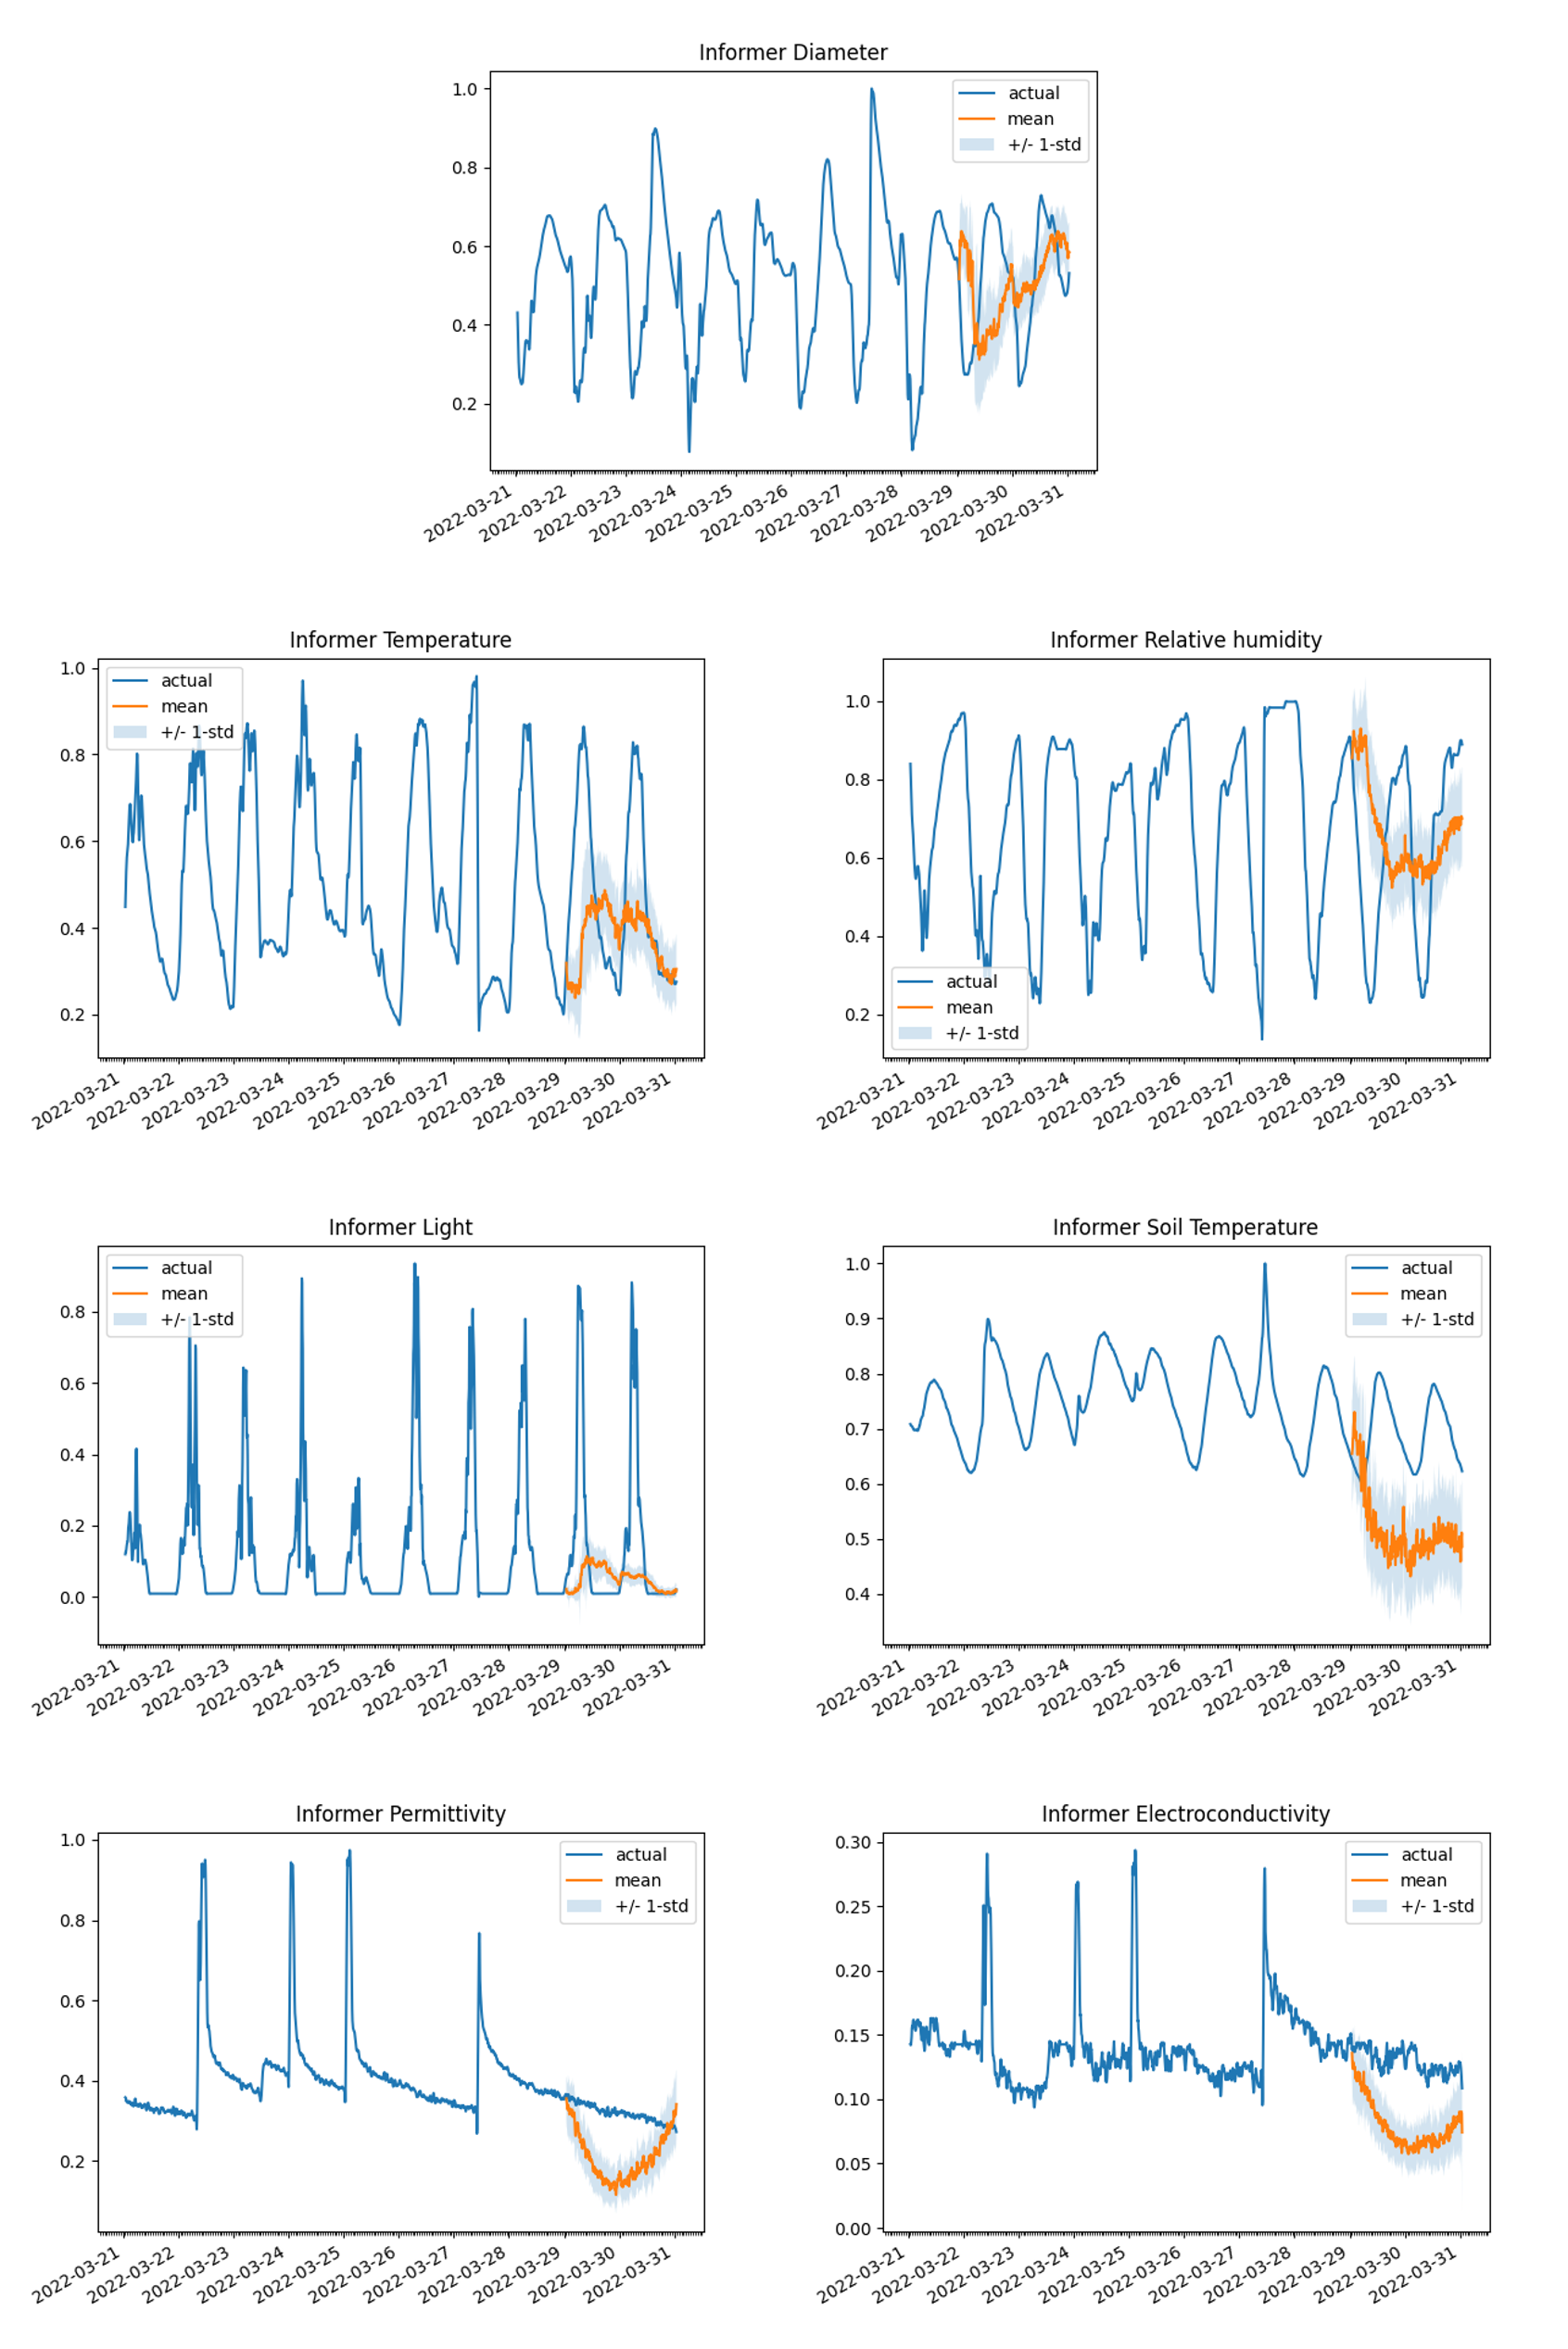
\includegraphics[width=15 cm]{6_ChapterResults/figuras/I3.png}
    \caption{Comparison between the predicted values generated by the I3 model and the actual observed values for the 7 variables over a two-day prediction horizon}
    \label{I3}
\end{figure}


\subsection{Autoformer}
The results for the Autoformer variant, as shown in Tables \ref{A1_M} and \ref{A1_R}, indicate better performance than the Transformer when more data is used, similar to the Informer. This demonstrates the Autoformer's strong scalability and ability to effectively manage larger Prediction Length and Context Length values.

Additionally, as seen in Table \ref{A1_T}, the Autoformer, like the Informer, is more efficient in terms of training time compared to the Transformer when working with large datasets. However, it's important to note that the Autoformer is not more efficient than the Informer in any of its models. Therefore, when comparing the three variants, the Informer stands out as the most computationally efficient model.

In Figure \ref{A3}, the predictions of the A3 model are compared with the actual observed values for the 7 variables. The figure demonstrates the model's precision over a two-day prediction period, providing a clear visual assessment of its performance across different variables.

\begin{table}[]
    \centering
    \resizebox{\textwidth}{!}{%
    \begin{tabular}{ccccccccc}
    \rowcolor[HTML]{FFFFFF} 
    \multicolumn{9}{c}{\cellcolor[HTML]{FFFFFF}\textbf{MSE   (Sorted by model)}}                                                                                                                                                                                                                       \\
    \rowcolor[HTML]{FFFFFF} 
    Model                      & Diameter                       & Electroconductivity            & Light                          & Permittivity                   & Relative\_humidity             & Soil\_Temperature              & Temperature                    & Mean                           \\
    \cellcolor[HTML]{FFFFFF}A1 & \cellcolor[HTML]{FEC97E}-20.51 & \cellcolor[HTML]{63BE7B}-40.48 & \cellcolor[HTML]{FCEA83}-11.84 & \cellcolor[HTML]{91CB7D}-37.39 & \cellcolor[HTML]{E0E282}-20.16 & \cellcolor[HTML]{6FC17B}-21.57 & \cellcolor[HTML]{FFE884}-21.91 & \cellcolor[HTML]{D4DE81}-24.84 \\
    \cellcolor[HTML]{FFFFFF}A2 & \cellcolor[HTML]{FA8170}-17.36 & \cellcolor[HTML]{B5D57F}-38.79 & \cellcolor[HTML]{63BE7B}-45.94 & \cellcolor[HTML]{63BE7B}-42.25 & \cellcolor[HTML]{63BE7B}-29.24 & \cellcolor[HTML]{FEEA83}-19.53 & \cellcolor[HTML]{FECF7F}-20.41 & \cellcolor[HTML]{63BE7B}-30.50 \\
    \cellcolor[HTML]{FFFFFF}A3 & \cellcolor[HTML]{63BE7B}-25.42 & \cellcolor[HTML]{FDBE7C}-35.20 & \cellcolor[HTML]{FEEA83}-11.44 & \cellcolor[HTML]{FAE983}-26.30 & \cellcolor[HTML]{FFEB84}-17.98 & \cellcolor[HTML]{63BE7B}-21.75 & \cellcolor[HTML]{6FC17B}-24.59 & \cellcolor[HTML]{F4E883}-23.24 \\
    \cellcolor[HTML]{FFFFFF}A4 & \cellcolor[HTML]{FFDA81}-21.25 & \cellcolor[HTML]{F8696B}-31.40 & \cellcolor[HTML]{FDEA83}-11.62 & \cellcolor[HTML]{FB8F73}-22.73 & \cellcolor[HTML]{F9E983}-18.41 & \cellcolor[HTML]{FAE983}-19.59 & \cellcolor[HTML]{8FCA7D}-24.03 & \cellcolor[HTML]{FDC27C}-21.29 \\
    \cellcolor[HTML]{FFFFFF}A5 & \cellcolor[HTML]{85C77C}-24.68 & \cellcolor[HTML]{95CC7D}-39.44 & \cellcolor[HTML]{FCAA78}-11.27 & \cellcolor[HTML]{FFE884}-25.68 & \cellcolor[HTML]{FED881}-17.00 & \cellcolor[HTML]{FFEB84}-19.52 & \cellcolor[HTML]{F3E783}-22.30 & \cellcolor[HTML]{FCEA83}-22.84 \\
    \cellcolor[HTML]{FFFFFF}A6 & \cellcolor[HTML]{DAE081}-22.83 & \cellcolor[HTML]{F1E783}-37.54 & \cellcolor[HTML]{FCAE79}-11.27 & \cellcolor[HTML]{FDEA83}-25.95 & \cellcolor[HTML]{FFEB84}-17.95 & \cellcolor[HTML]{FBA076}-18.12 & \cellcolor[HTML]{63BE7B}-24.81 & \cellcolor[HTML]{FFE984}-22.64 \\
    \rowcolor[HTML]{F8696B} 
    \cellcolor[HTML]{FFFFFF}A7 & -16.30                         & \cellcolor[HTML]{FECE7F}-35.93 & \cellcolor[HTML]{F9726D}-11.19 & -21.49                         & -11.42                         & -17.12                         & -14.34                         & -18.25                         \\
    \cellcolor[HTML]{FFFFFF}A8 & \cellcolor[HTML]{D5DF81}-22.94 & \cellcolor[HTML]{FFE583}-36.97 & \cellcolor[HTML]{F8696B}-11.18 & \cellcolor[HTML]{F9706D}-21.71 & \cellcolor[HTML]{FEEA83}-18.00 & \cellcolor[HTML]{FCA577}-18.22 & \cellcolor[HTML]{FED981}-20.99 & \cellcolor[HTML]{FDC67D}-21.43
    \end{tabular}%
    }
    \caption{Mean Squared Errors (MSE) for different Autoformer models obtained by varying the prediction length and context length, sorted by model}
    \label{A1_M}
    \end{table}


\begin{table}[]
    \centering
    \resizebox{\textwidth}{!}{%
    \begin{tabular}{ccccccccc}
    \rowcolor[HTML]{FFFFFF} 
    \multicolumn{9}{c}{\cellcolor[HTML]{FFFFFF}\textbf{R2 (Sorted by model)}}                                                                                                                                                                                                                  \\
    \rowcolor[HTML]{FFFFFF} 
    Model                      & Diameter                      & Electroconductivity           & Light                         & Permittivity                   & Relative\_humidity            & Soil\_Temperature             & Temperature                  & Mean                          \\
    \cellcolor[HTML]{FFFFFF}A1 & \cellcolor[HTML]{FEE282}0.59  & \cellcolor[HTML]{69C07C}-0.45 & \cellcolor[HTML]{63BE7B}-0.21 & \cellcolor[HTML]{6BC17C}-0.11  & \cellcolor[HTML]{63BE7B}0.82  & \cellcolor[HTML]{88C97E}-1.18 & \cellcolor[HTML]{FEEA83}0.83 & \cellcolor[HTML]{63BE7B}0.04  \\
    \rowcolor[HTML]{F8696B} 
    \cellcolor[HTML]{FFFFFF}A2 & -1.58                         & -6.21                         & -8.24                         & \cellcolor[HTML]{63BE7B}0.12   & \cellcolor[HTML]{A9D27F}0.76  & \cellcolor[HTML]{F98C71}-3.70 & -4.80                        & -3.38                         \\
    \cellcolor[HTML]{FFFFFF}A3 & \cellcolor[HTML]{63BE7B}0.87  & \cellcolor[HTML]{FDCF7E}-2.73 & \cellcolor[HTML]{A3D17F}-0.25 & \cellcolor[HTML]{F8E984}-4.12  & \cellcolor[HTML]{FEEA83}0.69  & \cellcolor[HTML]{63BE7B}-0.78 & \cellcolor[HTML]{6EC27C}0.91 & \cellcolor[HTML]{DEE283}-0.77 \\
    \cellcolor[HTML]{FFFFFF}A4 & \cellcolor[HTML]{FEEA83}0.74  & \cellcolor[HTML]{FBA276}-4.26 & \cellcolor[HTML]{FEEA83}-0.34 & \cellcolor[HTML]{DCE182}-3.32  & \cellcolor[HTML]{E1E383}0.71  & \cellcolor[HTML]{B4D680}-1.66 & \cellcolor[HTML]{7BC57D}0.91 & \cellcolor[HTML]{FEE983}-1.03 \\
    \cellcolor[HTML]{FFFFFF}A5 & \cellcolor[HTML]{84C87D}0.85  & \cellcolor[HTML]{63BE7B}-0.40 & \cellcolor[HTML]{EFE784}-0.31 & \cellcolor[HTML]{FEE382}-4.90  & \cellcolor[HTML]{FEE182}0.61  & \cellcolor[HTML]{D1DE82}-1.97 & \cellcolor[HTML]{EFE784}0.85 & \cellcolor[HTML]{DBE182}-0.75 \\
    \cellcolor[HTML]{FFFFFF}A6 & \cellcolor[HTML]{EDE683}0.77  & \cellcolor[HTML]{B8D780}-1.17 & \cellcolor[HTML]{ECE683}-0.30 & \cellcolor[HTML]{FEE883}-4.55  & \cellcolor[HTML]{FEEA83}0.68  & \cellcolor[HTML]{FCBB7A}-3.10 & \cellcolor[HTML]{63BE7B}0.92 & \cellcolor[HTML]{FBEA84}-0.97 \\
    \cellcolor[HTML]{FFFFFF}A7 & \cellcolor[HTML]{FCBD7B}-0.06 & \cellcolor[HTML]{FEE182}-2.15 & \cellcolor[HTML]{FEEA83}-0.33 & \cellcolor[HTML]{F8696B}-14.51 & \cellcolor[HTML]{F8696B}-0.43 & \cellcolor[HTML]{F8696B}-4.16 & \cellcolor[HTML]{FED880}0.06 & \cellcolor[HTML]{F8796E}-3.08 \\
    \cellcolor[HTML]{FFFFFF}A8 & \cellcolor[HTML]{E5E483}0.77  & \cellcolor[HTML]{DAE182}-1.47 & \cellcolor[HTML]{FEEA83}-0.33 & \cellcolor[HTML]{F8736C}-13.72 & \cellcolor[HTML]{FEEB84}0.69  & \cellcolor[HTML]{FCC37C}-3.00 & \cellcolor[HTML]{FEE983}0.80 & \cellcolor[HTML]{FBA276}-2.33
    \end{tabular}%
    }
    \caption{R-squared (R²) for different Autoformer models obtained by varying the prediction length and context length, sorted by model}
    \label{A1_R}
    \end{table}


\begin{table}[]
    \begin{tabular}{
    >{\columncolor[HTML]{FFFFFF}}c cc
    >{\columncolor[HTML]{FFFFFF}}c c}
    \multicolumn{2}{c}{\cellcolor[HTML]{FFFFFF}\textbf{Training   Time (Sorted by model)}} & \cellcolor[HTML]{FFFFFF} & \multicolumn{2}{c}{\cellcolor[HTML]{FFFFFF}\textbf{Training Time (Sorted   by training time)}} \\
    Model                  & \cellcolor[HTML]{FFFFFF}Training time {[}s{]}                 & \cellcolor[HTML]{FFFFFF} & Model                      & \cellcolor[HTML]{FFFFFF}Training time {[}s{]}                     \\
    A1                     & \cellcolor[HTML]{85C77C}268.74                                &                          & A2                         & \cellcolor[HTML]{63BE7B}263.36                                    \\
    A2                     & \cellcolor[HTML]{63BE7B}263.36                                &                          & A1                         & \cellcolor[HTML]{85C77C}268.74                                    \\
    A3                     & \cellcolor[HTML]{FFE784}290.26                                &                          & A5                         & \cellcolor[HTML]{D8DF81}281.66                                    \\
    A4                     & \cellcolor[HTML]{F8696B}372.63                                &                          & A6                         & \cellcolor[HTML]{EDE683}284.96                                    \\
    A5                     & \cellcolor[HTML]{D8DF81}281.66                                &                          & A3                         & \cellcolor[HTML]{FFE784}290.26                                    \\
    A6                     & \cellcolor[HTML]{EDE683}284.96                                &                          & A7                         & \cellcolor[HTML]{FCB079}326.78                                    \\
    A7                     & \cellcolor[HTML]{FCB079}326.78                                &                          & A8                         & \cellcolor[HTML]{FB9373}345.52                                    \\
    A8                     & \cellcolor[HTML]{FB9373}345.52                                &                          & A4                         & \cellcolor[HTML]{F8696B}372.63                                   
    \end{tabular}%
    \caption{Training times for different Autoformer models obtained by varying the prediction length and context length, sorted by model and training time values}
    \label{A1_T}
    \end{table}

\begin{figure}[htbp]
    \centering
    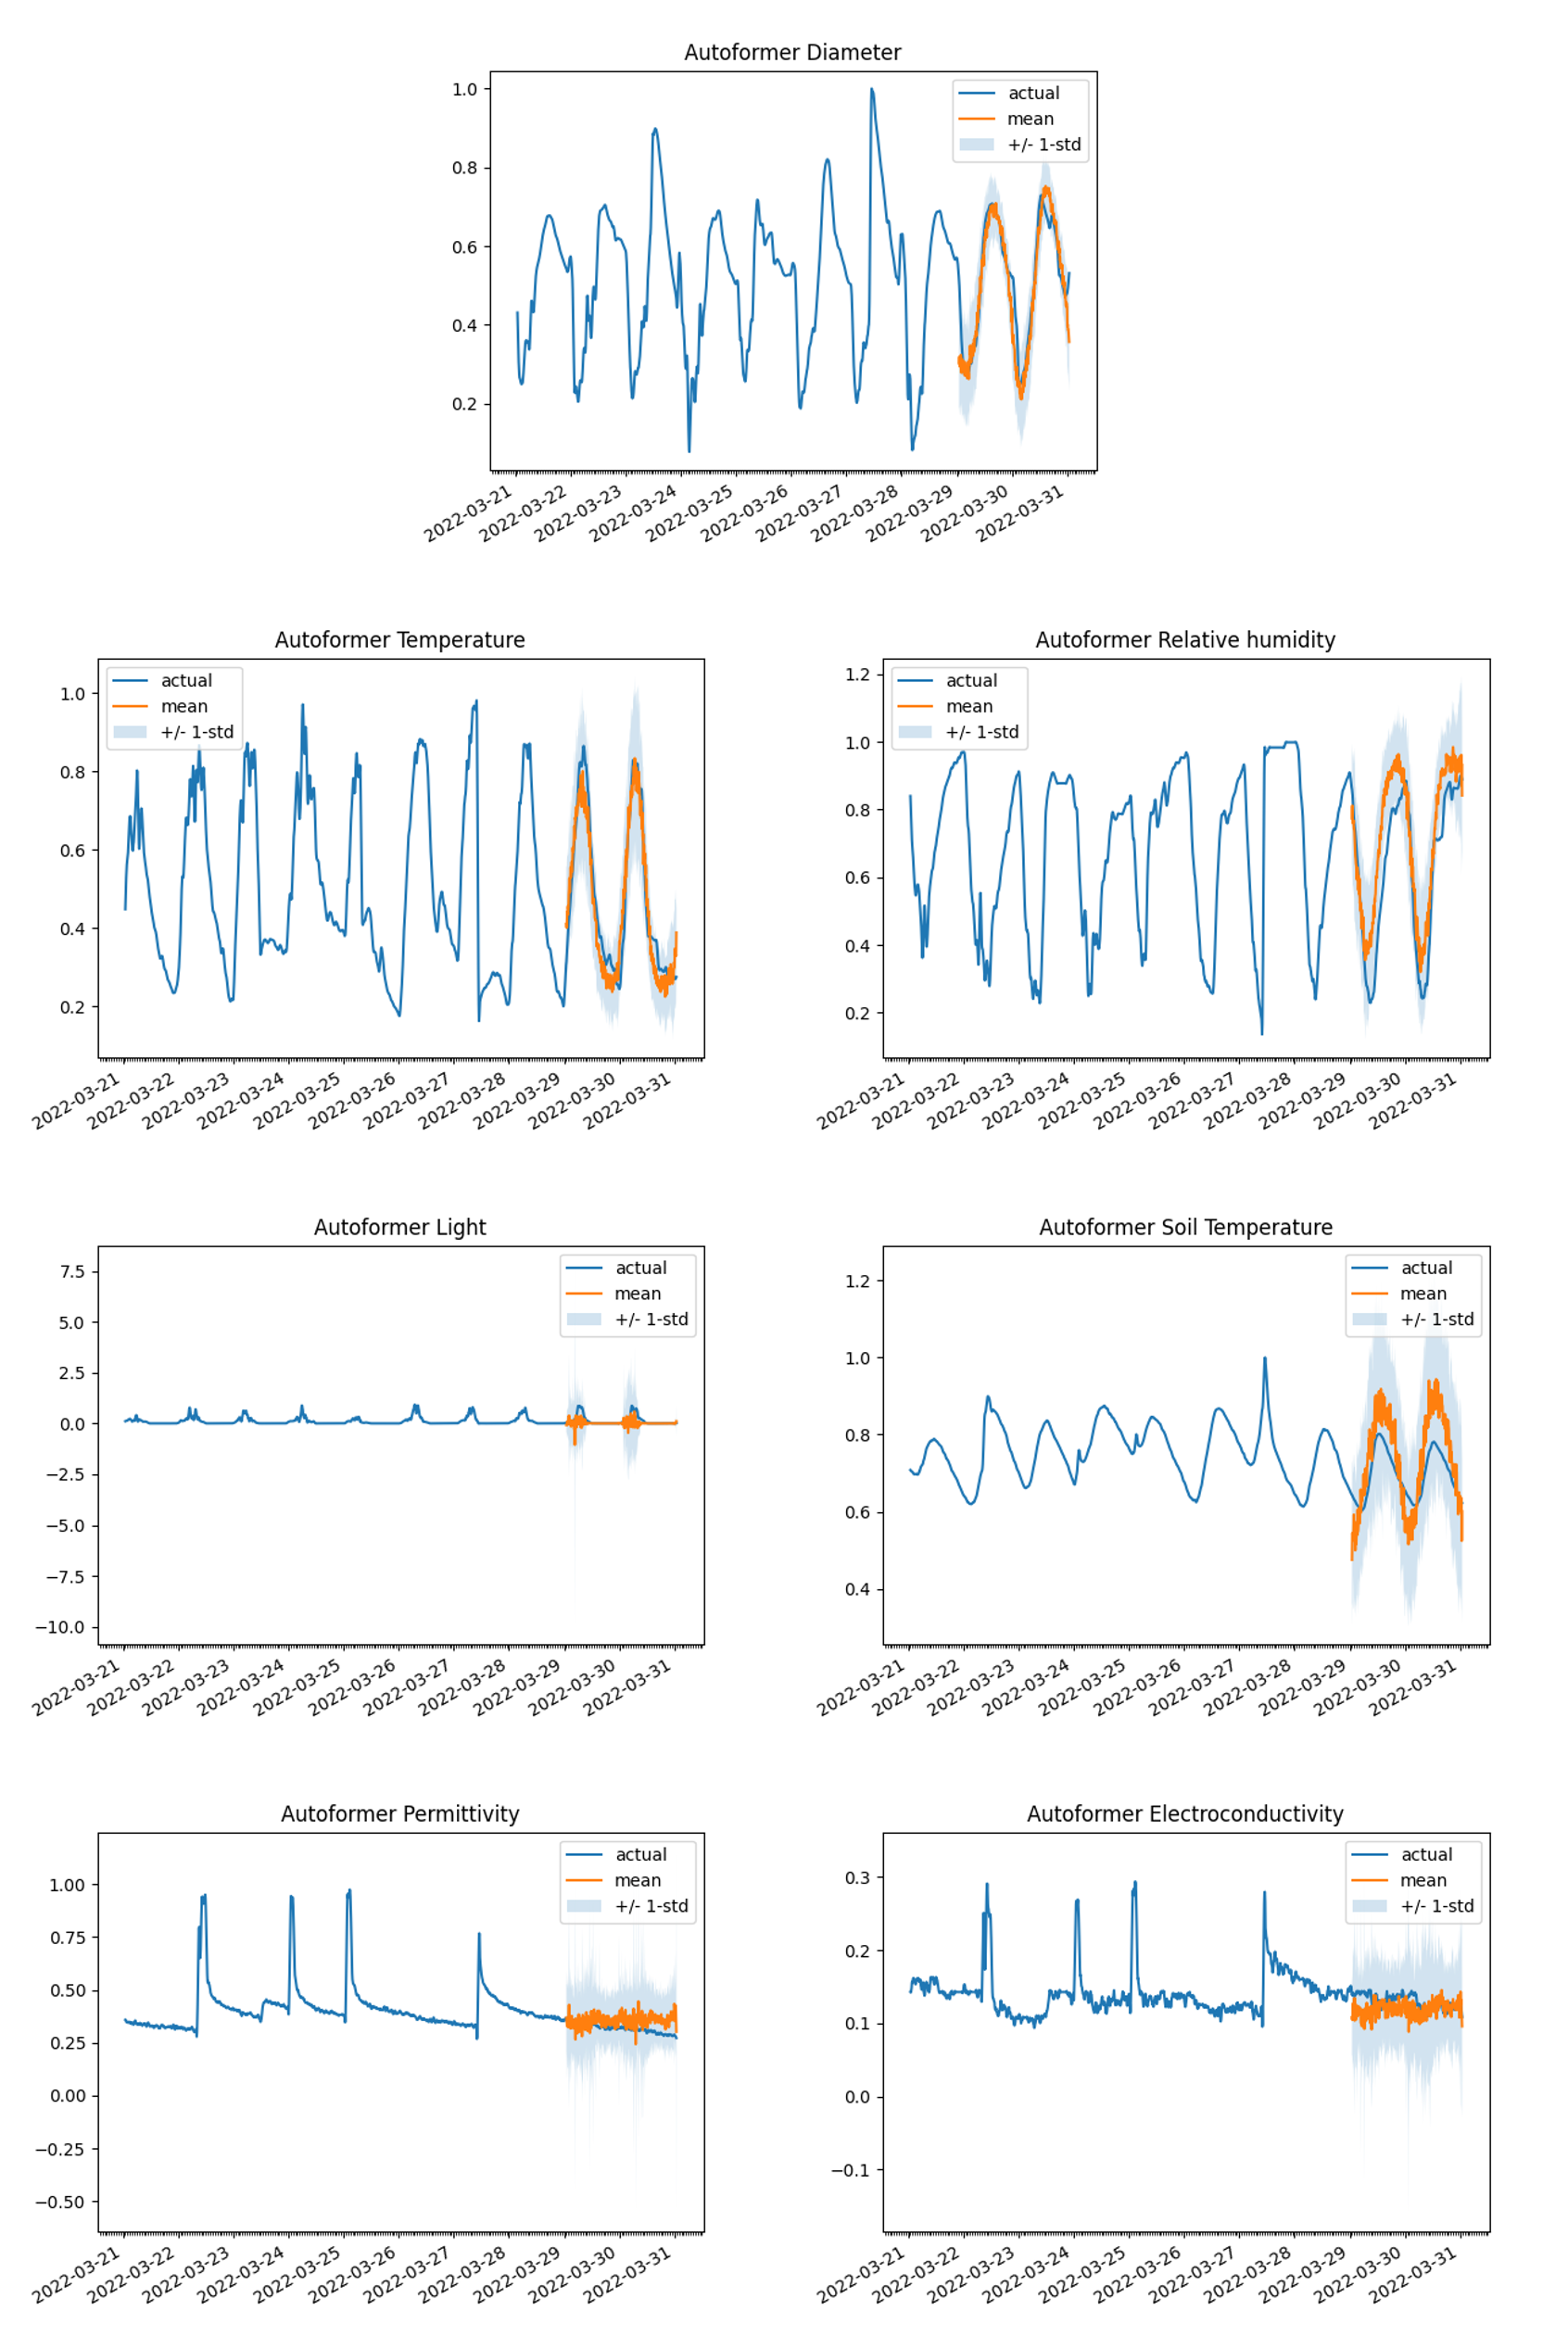
\includegraphics[width=15 cm]{6_ChapterResults/figuras/A3.png}
    \caption{Comparison between the predicted values generated by the A3 model and the actual observed values for the 7 variables over a two-day prediction horizon}
    \label{A3}
\end{figure}






\section{Results Changing the Lags Sequence}
In this section, we advance to the next phase of experimentation by focusing on models T3, I3, and A3, which were identified as the most practical in the previous phase. Here, we test these models with different values of Lags sequence to evaluate how variations in the lagged input data affect their predictive performance. This analysis aims to determine the optimal lag configuration that enhances model accuracy and utility, further refining our approach to time series forecasting.

\subsection{Transformer}
The results for the Transformer variant with added Lags Sequences, as shown in Tables \ref{T2_M} and \ref{T2_R}, indicate mixed outcomes. Compared to the original T3 model, which did not use any Lags Sequence, the performance deteriorates for models T9, T10, and T11. However, the results improve for models T12 and T13, suggesting that while smaller Lags Sequences might not be beneficial, a sufficiently large Lags Sequence can enhance the Transformer's predictive capabilities. Among all the models tested so far, we consider T13 to be the best, primarily due to its strong performance in predicting plant diameter.Figure \ref{T13} illustrates the comparison between the predictions generated by the T13 model and the actual observed values, highlighting the model's effectiveness.

On the other hand, as seen in Table \ref{T2_T}, the addition of Lags Sequences leads to increased training times, as working with Lags Sequences requires additional comparisons, resulting in a higher computational cost.


\begin{table}[]
    \centering
    \resizebox{\textwidth}{!}{%
    \begin{tabular}{ccccccccc}
    \rowcolor[HTML]{FFFFFF} 
    \multicolumn{9}{c}{\cellcolor[HTML]{FFFFFF}\textbf{MSE   (Sorted by model)}}                                                                                                                                                                                                                        \\
    \rowcolor[HTML]{FFFFFF} 
    Model                       & Diameter                       & Electroconductivity            & Light                          & Permittivity                   & Relative Humidity              & Soil Temperature               & Temperature                    & Mean                           \\
    \cellcolor[HTML]{FFFFFF}T9  & \cellcolor[HTML]{FB9D75}-17.25 & \cellcolor[HTML]{9FCF7E}-31.89 & \cellcolor[HTML]{FFEB84}-14.01 & \cellcolor[HTML]{F8696B}-17.64 & \cellcolor[HTML]{63BE7B}-14.98 & \cellcolor[HTML]{F96F6D}-12.27 & \cellcolor[HTML]{63BE7B}-18.33 & \cellcolor[HTML]{FFDD82}-18.05 \\
    \cellcolor[HTML]{FFFFFF}T10 & \cellcolor[HTML]{FFEB84}-19.55 & \cellcolor[HTML]{F8696B}-25.03 & \cellcolor[HTML]{FA8270}-13.33 & \cellcolor[HTML]{63BE7B}-31.58 & \cellcolor[HTML]{FFEB84}-14.16 & \cellcolor[HTML]{63BE7B}-22.43 & \cellcolor[HTML]{FFEB84}-16.63 & \cellcolor[HTML]{72C27B}-20.39 \\
    \rowcolor[HTML]{F8696B} 
    \cellcolor[HTML]{FFFFFF}T11 & -15.73                         & \cellcolor[HTML]{FFEB84}-27.28 & -13.18                         & \cellcolor[HTML]{FFEB84}-24.94 & -11.28                         & \cellcolor[HTML]{FFEB84}-16.59 & -15.22                         & -17.74                         \\
    \cellcolor[HTML]{FFFFFF}T12 & \cellcolor[HTML]{88C87D}-21.92 & \cellcolor[HTML]{63BE7B}-34.80 & \cellcolor[HTML]{63BE7B}-14.11 & \cellcolor[HTML]{C0D880}-27.61 & \cellcolor[HTML]{FECD7F}-13.49 & \cellcolor[HTML]{ECE582}-17.30 & \cellcolor[HTML]{F96A6C}-15.23 & \cellcolor[HTML]{63BE7B}-20.64 \\
    \cellcolor[HTML]{FFFFFF}T13 & \cellcolor[HTML]{63BE7B}-22.65 & \cellcolor[HTML]{F9766E}-25.25 & \cellcolor[HTML]{ABD27F}-14.06 & \cellcolor[HTML]{FCAC78}-21.35 & \cellcolor[HTML]{DAE081}-14.35 & \cellcolor[HTML]{F8696B}-12.06 & \cellcolor[HTML]{E3E382}-16.92 & \cellcolor[HTML]{FFEB84}-18.09
    \end{tabular}%
    }
    \caption{Mean Squared Errors (MSE) for different Transformer models obtained by varying the Lags Sequence values, sorted by model}
    \label{T2_M}
    \end{table}

\begin{table}[]
    \centering
    \resizebox{\textwidth}{!}{%
    \begin{tabular}{ccccccccc}
    \rowcolor[HTML]{FFFFFF} 
    \multicolumn{9}{c}{\cellcolor[HTML]{FFFFFF}\textbf{R2 (Sorted by model)}}                                                                                                                                                                                                                    \\
    \rowcolor[HTML]{FFFFFF} 
    Model                       & Diameter                      & Electroconductivity            & Light                        & Permittivity                   & Relative\_humidity            & Soil\_Temperature              & Temperature                  & Mean                          \\
    \cellcolor[HTML]{FFFFFF}T9  & \cellcolor[HTML]{FBAA77}0.15  & \cellcolor[HTML]{83C87D}-6.98  & \cellcolor[HTML]{FFEB84}0.31 & \cellcolor[HTML]{F8696B}-36.60 & \cellcolor[HTML]{63BE7B}0.37  & \cellcolor[HTML]{F8726C}-14.78 & \cellcolor[HTML]{63BE7B}0.63 & \cellcolor[HTML]{F98D72}-8.13 \\
    \cellcolor[HTML]{FFFFFF}T10 & \cellcolor[HTML]{FFEB84}0.50  & \cellcolor[HTML]{F8696B}-37.71 & \cellcolor[HTML]{F9826F}0.19 & \cellcolor[HTML]{63BE7B}-0.52  & \cellcolor[HTML]{FFEB84}0.24  & \cellcolor[HTML]{63BE7B}-0.52  & \cellcolor[HTML]{FFEB84}0.45 & \cellcolor[HTML]{FFEB84}-5.34 \\
    \cellcolor[HTML]{FFFFFF}T11 & \cellcolor[HTML]{F8696B}-0.21 & \cellcolor[HTML]{FFEB84}-22.07 & \cellcolor[HTML]{F8696B}0.16 & \cellcolor[HTML]{FFEB84}-6.00  & \cellcolor[HTML]{F8696B}-0.47 & \cellcolor[HTML]{FFEB84}-4.83  & \cellcolor[HTML]{F8696B}0.23 & \cellcolor[HTML]{E9E583}-4.74 \\
    \cellcolor[HTML]{FFFFFF}T12 & \cellcolor[HTML]{7FC67D}0.71  & \cellcolor[HTML]{63BE7B}-3.08  & \cellcolor[HTML]{63BE7B}0.32 & \cellcolor[HTML]{A4D17F}-2.79  & \cellcolor[HTML]{FDD47F}0.12  & \cellcolor[HTML]{E0E283}-3.96  & \cellcolor[HTML]{F86A6B}0.23 & \cellcolor[HTML]{63BE7B}-1.21 \\
    \cellcolor[HTML]{FFFFFF}T13 & \cellcolor[HTML]{63BE7B}0.76  & \cellcolor[HTML]{F8786E}-35.83 & \cellcolor[HTML]{A8D27F}0.32 & \cellcolor[HTML]{FCC47C}-15.01 & \cellcolor[HTML]{D8E082}0.27  & \cellcolor[HTML]{F8696B}-15.53 & \cellcolor[HTML]{DFE283}0.48 & \cellcolor[HTML]{F8696B}-9.22
    \end{tabular}%
    }
    \caption{R-squared (R²) for different Transformer models obtained by varying the Lags Sequence values, sorted by model}
    \label{T2_R}
    \end{table}


\begin{table}[]
    \begin{tabular}{ccccc}
    \multicolumn{2}{c}{\cellcolor[HTML]{FFFFFF}\textbf{Training   Time (Sorted by model)}} &  & \multicolumn{2}{c}{\cellcolor[HTML]{FFFFFF}\textbf{Training Time (Sorted   by training time)}} \\
    Model                         & Training time {[}s{]}                                  &  & Model                             & Training time {[}s{]}                                      \\
    T9                            & \cellcolor[HTML]{63BE7B}246.61                         &  & T9                                & \cellcolor[HTML]{63BE7B}246.61                             \\
    T10                           & \cellcolor[HTML]{E5E382}255.4                          &  & T10                               & \cellcolor[HTML]{E5E382}255.4                              \\
    T11                           & \cellcolor[HTML]{F8696B}260.8                          &  & T13                               & \cellcolor[HTML]{FFEB84}257.08                             \\
    T12                           & \cellcolor[HTML]{FFEA84}257.13                         &  & T12                               & \cellcolor[HTML]{FFEA84}257.13                             \\
    T13                           & \cellcolor[HTML]{FFEB84}257.08                         &  & T11                               & \cellcolor[HTML]{F8696B}260.8                             
    \end{tabular}%
    \caption{Training times for different Transformer models obtained  by varying the Lags Sequence values, sorted by model and training time values}
    \label{T2_T}
    \end{table}

\begin{figure}[htbp]
    \centering
    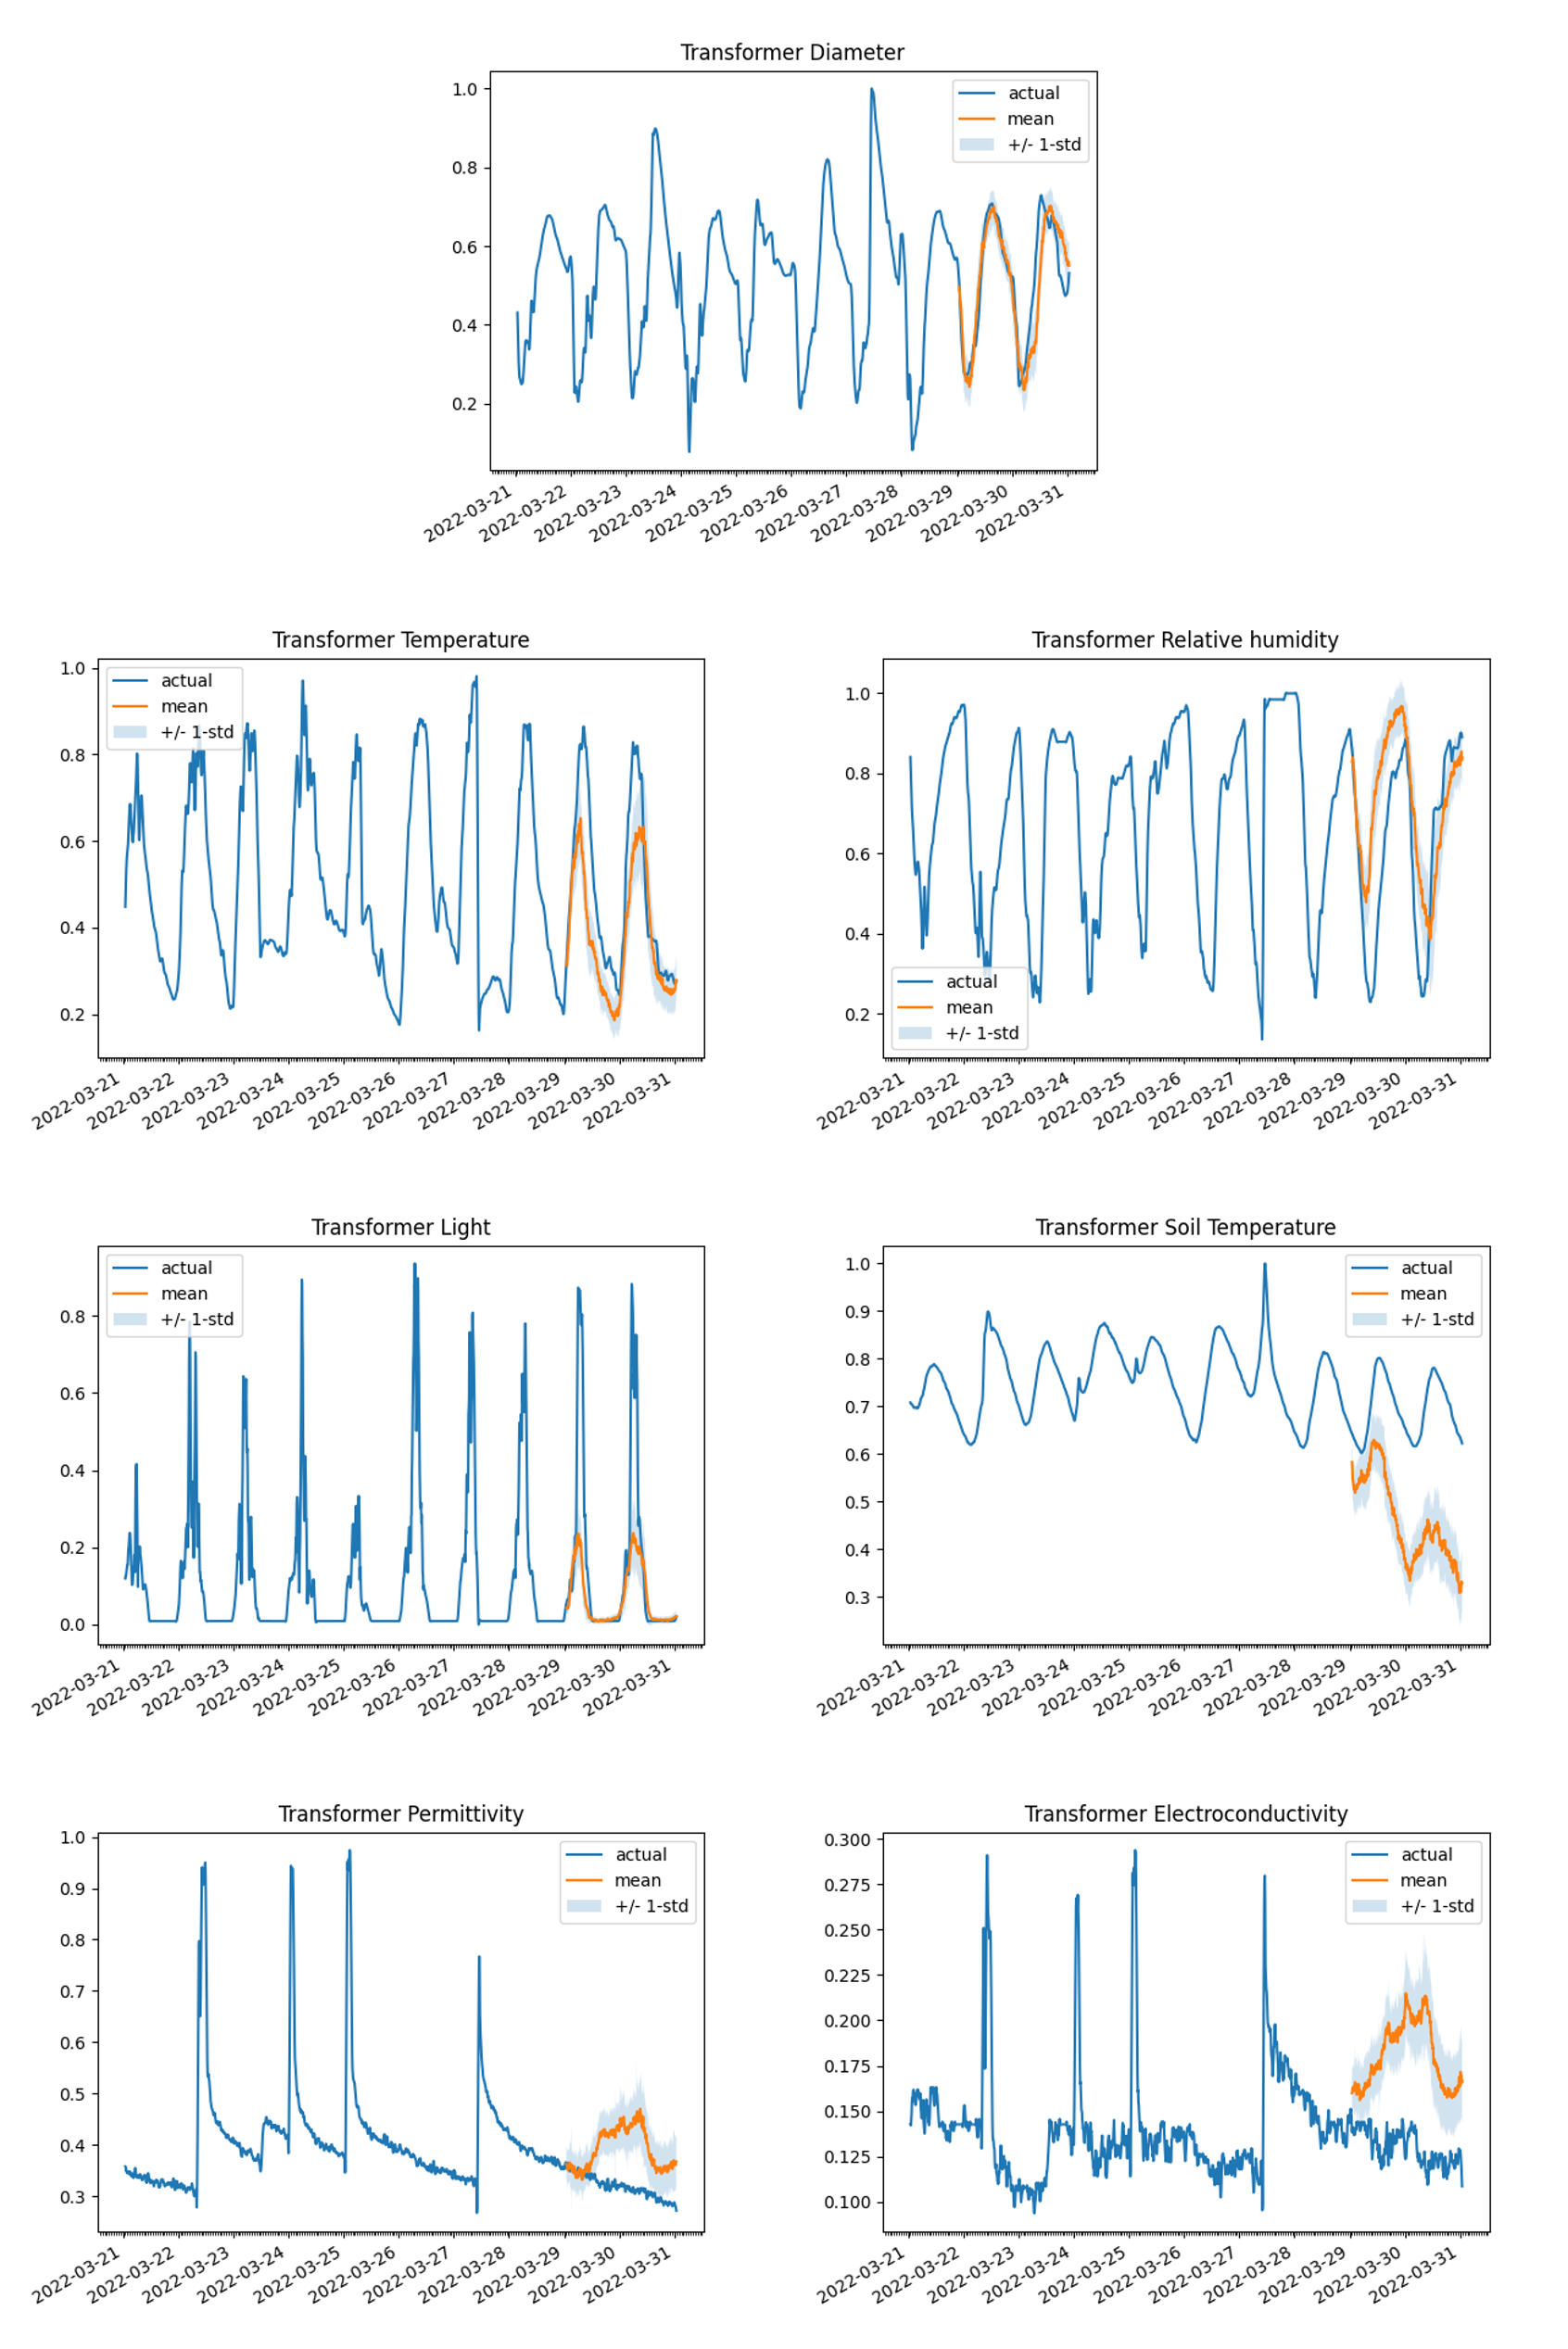
\includegraphics[width=15 cm]{6_ChapterResults/figuras/T13.png}
    \caption{Comparison between the predicted values generated by the T13 model and the actual observed values for the 7 variables over a two-day prediction horizon}
    \label{T13}
\end{figure}
    

\subsection{Informer}
The results for the Informer variant with added Lags Sequences, as shown in Tables \ref{I2_M} and \ref{I2_R}, demonstrate an improvement across all models compared to the original I3 model, which did not use any Lags Sequence. Each model that incorporates Lags Sequences shows better performance, indicating that this approach is beneficial for the Informer architecture. Once again, I13 has been chosen as the best overall model, not only for its strong performance in predicting plant diameter but also for its accuracy in forecasting other variables. Figure \ref{I13} illustrates the comparison between the predictions generated by the I13 model and the actual observed values, highlighting the model's effectiveness.

Additionally, as seen in Table \ref{I2_T}, the Informer variant proves to be more computationally efficient than the Transformer, reducing training times even with the added complexity of Lags Sequences.

\begin{table}[]
    \centering
    \resizebox{\textwidth}{!}{%
    \begin{tabular}{ccccccccc}
    \multicolumn{9}{c}{\textbf{MSE   (Sorted by model)}}                                                                                                                                                                                                                          \\
    Model & Diameter                       & Electroconductivity            & Light                          & Permittivity                   & Relative\_humidity             & Soil\_Temperature              & Temperature                    & Mean                           \\
    I9    & \cellcolor[HTML]{F8696B}-17.16 & \cellcolor[HTML]{FFEB84}-29.00 & \cellcolor[HTML]{FFEB84}-12.54 & \cellcolor[HTML]{FDBB7B}-17.83 & \cellcolor[HTML]{FFEB84}-11.75 & \cellcolor[HTML]{FB9073}-11.63 & \cellcolor[HTML]{75C37C}-15.37 & \cellcolor[HTML]{F8696B}-16.47 \\
    I10   & \cellcolor[HTML]{CBDC81}-20.80 & \cellcolor[HTML]{FFEB84}-29.01 & \cellcolor[HTML]{63BE7B}-13.14 & \cellcolor[HTML]{F8696B}-17.25 & \cellcolor[HTML]{FDBC7B}-11.24 & \cellcolor[HTML]{FFEB84}-15.74 & \cellcolor[HTML]{63BE7B}-15.40 & \cellcolor[HTML]{FCB37A}-17.51 \\
    I11   & \cellcolor[HTML]{FFEB84}-20.70 & \cellcolor[HTML]{F8696B}-24.60 & \cellcolor[HTML]{FFDC82}-12.49 & \cellcolor[HTML]{9DCE7E}-25.99 & \cellcolor[HTML]{63BE7B}-12.61 & \cellcolor[HTML]{E7E482}-16.73 & \cellcolor[HTML]{FFEB84}-15.16 & \cellcolor[HTML]{FFEB84}-18.32 \\
    I12   & \cellcolor[HTML]{63BE7B}-21.01 & \cellcolor[HTML]{91CB7D}-34.80 & \cellcolor[HTML]{D5DF81}-12.70 & \cellcolor[HTML]{63BE7B}-30.64 & \cellcolor[HTML]{B2D47F}-12.17 & \cellcolor[HTML]{F8696B}-9.89  & \cellcolor[HTML]{F8696B}-11.77 & \cellcolor[HTML]{63BE7B}-19.00 \\
    I13   & \cellcolor[HTML]{FBA076}-18.64 & \cellcolor[HTML]{63BE7B}-37.29 & \cellcolor[HTML]{F8696B}-12.05 & \cellcolor[HTML]{FFEB84}-18.17 & \cellcolor[HTML]{F8696B}-10.35 & \cellcolor[HTML]{63BE7B}-22.38 & \cellcolor[HTML]{FCA878}-13.41 & \cellcolor[HTML]{79C47C}-18.90
    \end{tabular}%
    }
    \caption{Mean Squared Errors (MSE) for different Informer models obtained by varying the Lags Sequence values, sorted by model}
    \label{I2_M}
    \end{table}

\begin{table}[]
    \centering
    \resizebox{\textwidth}{!}{%
    \begin{tabular}{ccccccccc}
    \multicolumn{9}{c}{\textbf{R2 (Sorted by model)}}                                                                                                                                                                                                                       \\
    Model & Diameter                     & Electroconductivity            & Light                         & Permittivity                   & Relative\_humidity            & Soil\_Temperature              & Temperature                   & Mean                          \\
    I9    & \cellcolor[HTML]{F8696B}0.13 & \cellcolor[HTML]{FEEA83}-14.51 & \cellcolor[HTML]{FFEB84}0.03  & \cellcolor[HTML]{FCBD7B}-35.01 & \cellcolor[HTML]{FFEB84}-0.32 & \cellcolor[HTML]{FBA276}-17.29 & \cellcolor[HTML]{76C47D}0.26  & \cellcolor[HTML]{F8696B}-9.53 \\
    I10   & \cellcolor[HTML]{C9DC81}0.63 & \cellcolor[HTML]{FFEB84}-14.49 & \cellcolor[HTML]{63BE7B}0.15  & \cellcolor[HTML]{F8696B}-40.09 & \cellcolor[HTML]{FCC07B}-0.49 & \cellcolor[HTML]{FFEB84}-6.09  & \cellcolor[HTML]{63BE7B}0.26  & \cellcolor[HTML]{FA9C74}-8.59 \\
    I11   & \cellcolor[HTML]{FFEB84}0.62 & \cellcolor[HTML]{F8696B}-41.77 & \cellcolor[HTML]{FEDC81}0.01  & \cellcolor[HTML]{75C47D}-4.49  & \cellcolor[HTML]{63BE7B}-0.09 & \cellcolor[HTML]{D7E082}-4.65  & \cellcolor[HTML]{FFEB84}0.22  & \cellcolor[HTML]{FFEB84}-7.16 \\
    I12   & \cellcolor[HTML]{63BE7B}0.64 & \cellcolor[HTML]{79C57D}-3.08  & \cellcolor[HTML]{D4DF82}0.06  & \cellcolor[HTML]{63BE7B}-0.88  & \cellcolor[HTML]{AFD480}-0.20 & \cellcolor[HTML]{F8696B}-26.30 & \cellcolor[HTML]{F8696B}-0.70 & \cellcolor[HTML]{63BE7B}-4.35 \\
    I13   & \cellcolor[HTML]{FBAC77}0.38 & \cellcolor[HTML]{63BE7B}-1.30  & \cellcolor[HTML]{F8696B}-0.09 & \cellcolor[HTML]{FFEB84}-32.31 & \cellcolor[HTML]{F8696B}-0.83 & \cellcolor[HTML]{63BE7B}-0.54  & \cellcolor[HTML]{FCB479}-0.16 & \cellcolor[HTML]{86C97E}-4.98
    \end{tabular}%
    }
    \caption{R-squared (R²) for different Informer models obtained by varying the Lags Sequence values, sorted by model}
    \label{I2_R}
    \end{table}


\begin{table}[]
    \begin{tabular}{ccccc}
    \multicolumn{2}{c}{\textbf{Training   Time (Sorted by model)}} &  & \multicolumn{2}{c}{\textbf{Training Time (Sorted   by training time)}} \\
    Model             & Training time {[}s{]}                      &  & Model                 & Training time {[}s{]}                          \\
    I9                & \cellcolor[HTML]{63BE7B}128.38             &  & I9                    & \cellcolor[HTML]{63BE7B}128.38                 \\
    I10               & \cellcolor[HTML]{FB9374}149.6              &  & I10                   & \cellcolor[HTML]{FB9374}149.6                  \\
    I11               & \cellcolor[HTML]{F8696B}154.53             &  & I11                   & \cellcolor[HTML]{F8696B}154.53                 \\
    I12               & \cellcolor[HTML]{A4D07E}132.9              &  & I12                   & \cellcolor[HTML]{A4D07E}132.9                  \\
    I13               & \cellcolor[HTML]{FFEB84}139.2              &  & I13                   & \cellcolor[HTML]{FFEB84}139.2                 
    \end{tabular}
    \caption{Training times for different Informer models obtained  by varying the Lags Sequence values, sorted by model and training time values}
    \label{I2_T}
    \end{table}

\begin{figure}[htbp]
    \centering
    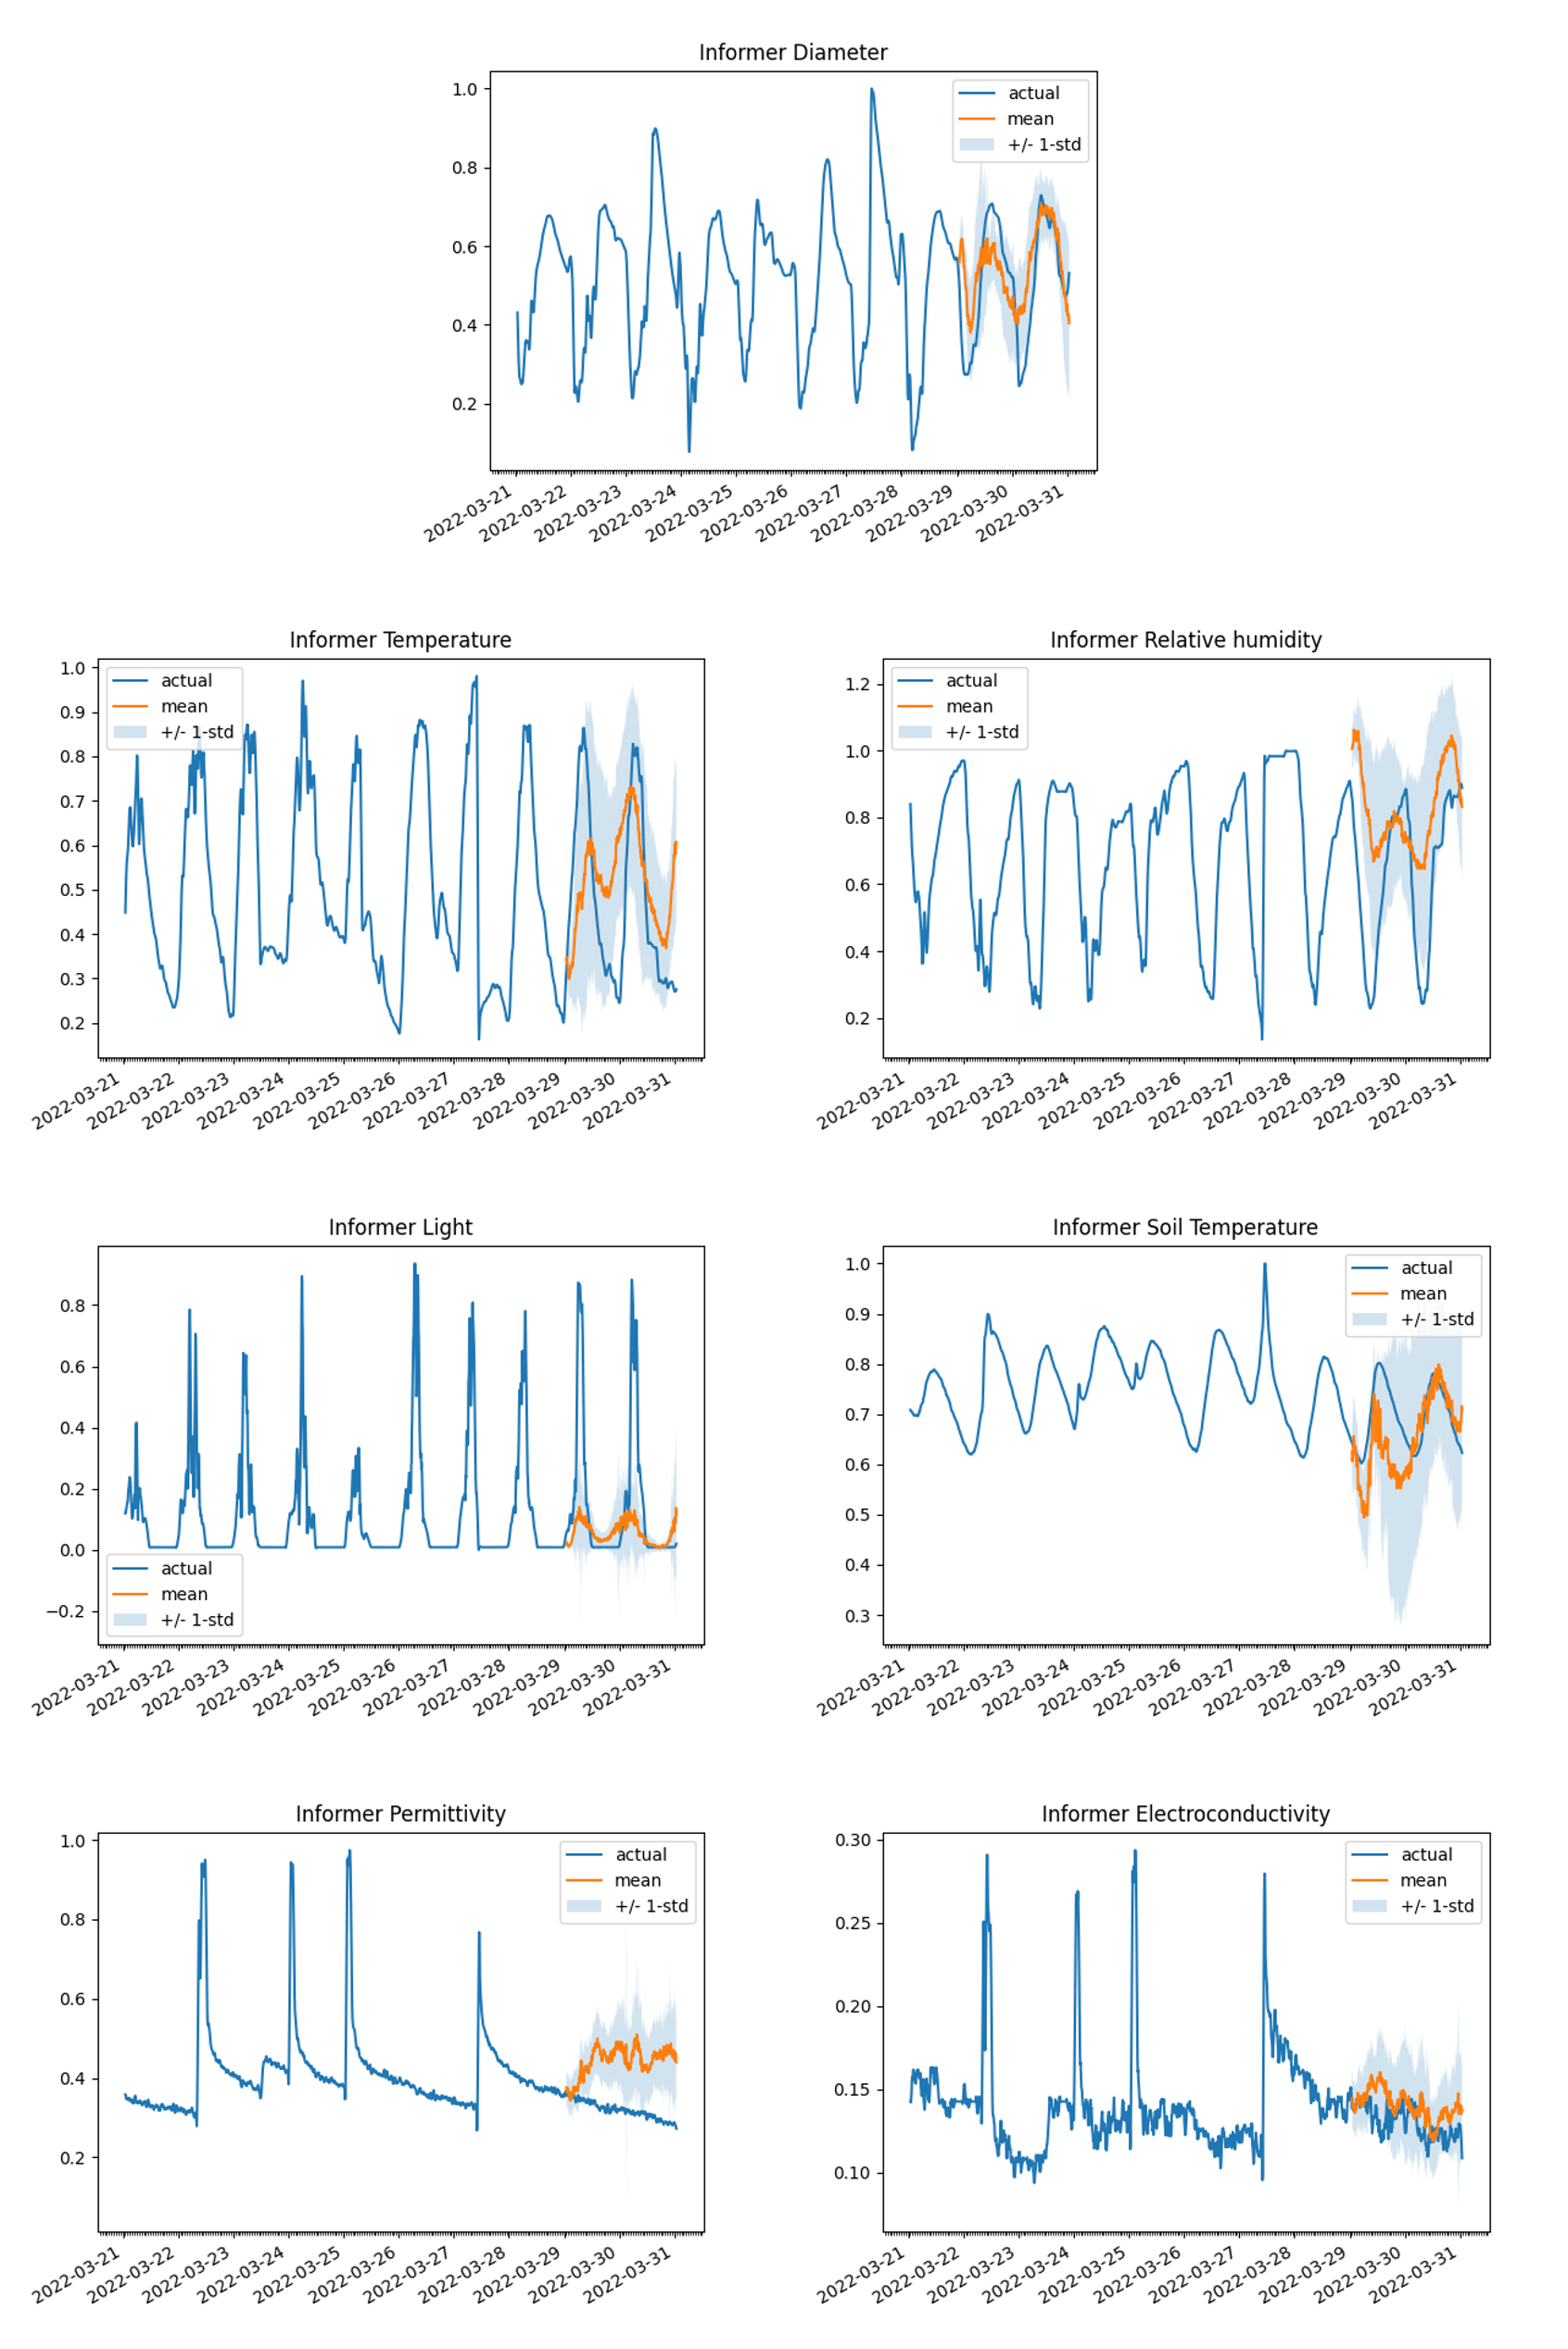
\includegraphics[width=15 cm]{6_ChapterResults/figuras/I13.png}
    \caption{Comparison between the predicted values generated by the I13 model and the actual observed values for the 7 variables over a two-day prediction horizon}
    \label{I13}
\end{figure}

\subsection{Autoformer}
The results for the Autoformer variant with added Lags Sequences, as shown in Tables \ref{A2_M} and \ref{A2_R}, reveal a significant improvement compared to the original A3 model, which did not utilize any Lags Sequence. This enhancement is particularly notable in the prediction of environmental variables, demonstrating the effectiveness of Lags Sequences in boosting the model's overall accuracy. Among the models tested, A11 is considered the best so far, due to its superior performance across key metrics. Figure \ref{A11} illustrates the comparison between the predictions generated by the A11 model and the actual observed values, highlighting the model's effectiveness.

However, as observed in Table \ref{A2_T}, there is an increase in computational cost, similar to what was seen with the Transformer and Informer variants. The addition of Lags Sequences requires more computational resources, leading to longer training times.


\begin{table}[]
    \centering
    \resizebox{\textwidth}{!}{%
    \begin{tabular}{ccccccccc}
    \multicolumn{9}{c}{\textbf{MSE   (Sorted by model)}}                                                                                                                                                                                                                          \\
    Model & Diameter                       & Electroconductivity            & Light                          & Permittivity                   & Relative\_humidity             & Soil\_Temperature              & Temperature                    & Mean                           \\
    A9    & \cellcolor[HTML]{63BE7B}-25.58 & \cellcolor[HTML]{FFEB84}-36.22 & \cellcolor[HTML]{FB9C75}-11.17 & \cellcolor[HTML]{FFEB84}-22.81 & \cellcolor[HTML]{FDC07C}-17.45 & \cellcolor[HTML]{FCA276}-20.25 & \cellcolor[HTML]{C4DA80}-22.55 & \cellcolor[HTML]{FFEB84}-22.29 \\
    A10   & \cellcolor[HTML]{FFEB84}-24.50 & \cellcolor[HTML]{94CC7D}-38.19 & \cellcolor[HTML]{F8696B}-11.10 & \cellcolor[HTML]{63BE7B}-24.76 & \cellcolor[HTML]{F8696B}-16.62 & \cellcolor[HTML]{F8696B}-20.06 & \cellcolor[HTML]{F8696B}-21.00 & \cellcolor[HTML]{F9E983}-22.32 \\
    A11   & \cellcolor[HTML]{D1DD81}-24.81 & \cellcolor[HTML]{63BE7B}-39.10 & \cellcolor[HTML]{FFEB84}-11.27 & \cellcolor[HTML]{8BC97D}-24.25 & \cellcolor[HTML]{63BE7B}-18.67 & \cellcolor[HTML]{63BE7B}-21.70 & \cellcolor[HTML]{FDB67A}-21.38 & \cellcolor[HTML]{63BE7B}-23.03 \\
    A12   & \cellcolor[HTML]{FB9E76}-23.22 & \cellcolor[HTML]{FCAF79}-32.57 & \cellcolor[HTML]{63BE7B}-11.38 & \cellcolor[HTML]{FB9E76}-20.65 & \cellcolor[HTML]{FFEB84}-17.87 & \cellcolor[HTML]{FFEB84}-20.49 & \cellcolor[HTML]{63BE7B}-24.07 & \cellcolor[HTML]{FCB37A}-21.47 \\
    A13   & \cellcolor[HTML]{F8696B}-22.35 & \cellcolor[HTML]{F8696B}-28.35 & \cellcolor[HTML]{A8D27F}-11.33 & \cellcolor[HTML]{F8696B}-19.21 & \cellcolor[HTML]{88C87D}-18.48 & \cellcolor[HTML]{88C87D}-21.41 & \cellcolor[HTML]{FFEB84}-21.64 & \cellcolor[HTML]{F8696B}-20.40
    \end{tabular}%
    }
    \caption{Mean Squared Errors (MSE) for different Autoformer models obtained by varying the Lags Sequence values, sorted by model}
    \label{A2_M}
    \end{table}

\begin{table}[]
    \centering
    \resizebox{\textwidth}{!}{%
    \begin{tabular}{ccccccccc}
    \multicolumn{9}{c}{\textbf{R2 (Sorted by model)}}                                                                                                                                                                                                                    \\
    Model & Diameter                     & Electroconductivity            & Light                         & Permittivity                   & Relative\_humidity           & Soil\_Temperature             & Temperature                  & Mean                          \\
    A9    & \cellcolor[HTML]{63BE7B}0.88 & \cellcolor[HTML]{FFEB84}-1.94  & \cellcolor[HTML]{FA9C74}-0.34 & \cellcolor[HTML]{FFEB84}-10.44 & \cellcolor[HTML]{FCC37C}0.64 & \cellcolor[HTML]{FBA376}-1.51 & \cellcolor[HTML]{BBD881}0.86 & \cellcolor[HTML]{FFEB84}-1.69 \\
    A10   & \cellcolor[HTML]{FFEB84}0.84 & \cellcolor[HTML]{8ACA7E}-0.87  & \cellcolor[HTML]{F8696B}-0.36 & \cellcolor[HTML]{63BE7B}-6.30  & \cellcolor[HTML]{F8696B}0.57 & \cellcolor[HTML]{F8696B}-1.62 & \cellcolor[HTML]{F8696B}0.80 & \cellcolor[HTML]{72C37C}-0.99 \\
    A11   & \cellcolor[HTML]{CEDD82}0.85 & \cellcolor[HTML]{63BE7B}-0.52  & \cellcolor[HTML]{FFEB84}-0.30 & \cellcolor[HTML]{85C87D}-7.20  & \cellcolor[HTML]{63BE7B}0.73 & \cellcolor[HTML]{63BE7B}-0.80 & \cellcolor[HTML]{FCB77A}0.81 & \cellcolor[HTML]{63BE7B}-0.92 \\
    A12   & \cellcolor[HTML]{FBA476}0.79 & \cellcolor[HTML]{FDC97D}-5.82  & \cellcolor[HTML]{63BE7B}-0.27 & \cellcolor[HTML]{FBAA77}-17.79 & \cellcolor[HTML]{FFEB84}0.68 & \cellcolor[HTML]{FFEB84}-1.38 & \cellcolor[HTML]{63BE7B}0.90 & \cellcolor[HTML]{FCBA7A}-3.27 \\
    A13   & \cellcolor[HTML]{F8696B}0.74 & \cellcolor[HTML]{F8696B}-17.02 & \cellcolor[HTML]{A8D27F}-0.29 & \cellcolor[HTML]{F8696B}-25.21 & \cellcolor[HTML]{88C97E}0.72 & \cellcolor[HTML]{85C87D}-0.92 & \cellcolor[HTML]{FFEB84}0.83 & \cellcolor[HTML]{F8696B}-5.88
    \end{tabular}%
    }
    \caption{R-squared (R²) for different Autoformer models obtained by varying the Lags Sequence values, sorted by model}
    \label{A2_R}
    \end{table}


\begin{table}[]
    \begin{tabular}{ccccc}
    \multicolumn{2}{c}{\textbf{Training   Time (Sorted by model)}} &  & \multicolumn{2}{c}{\textbf{Training Time (Sorted   by training time)}} \\
    Model             & Training time {[}s{]}                      &  & Model                 & Training time {[}s{]}                          \\
    A9                & \cellcolor[HTML]{63BE7B}299.49             &  & A9                    & \cellcolor[HTML]{63BE7B}299.49                 \\
    A10               & \cellcolor[HTML]{CEDD81}307.03             &  & A10                   & \cellcolor[HTML]{CEDD81}307.03                 \\
    A11               & \cellcolor[HTML]{F8696B}321.64             &  & A13                   & \cellcolor[HTML]{FFEB84}310.43                 \\
    A12               & \cellcolor[HTML]{FFEA84}310.6              &  & A12                   & \cellcolor[HTML]{FFEA84}310.6                  \\
    A13               & \cellcolor[HTML]{FFEB84}310.43             &  & A11                   & \cellcolor[HTML]{F8696B}321.64                
    \end{tabular}
    \caption{Training times for different Autoformer models obtained  by varying the Lags Sequence values, sorted by model and training time values}
    \label{A2_T}
    \end{table}


\begin{figure}[htbp]
    \centering
    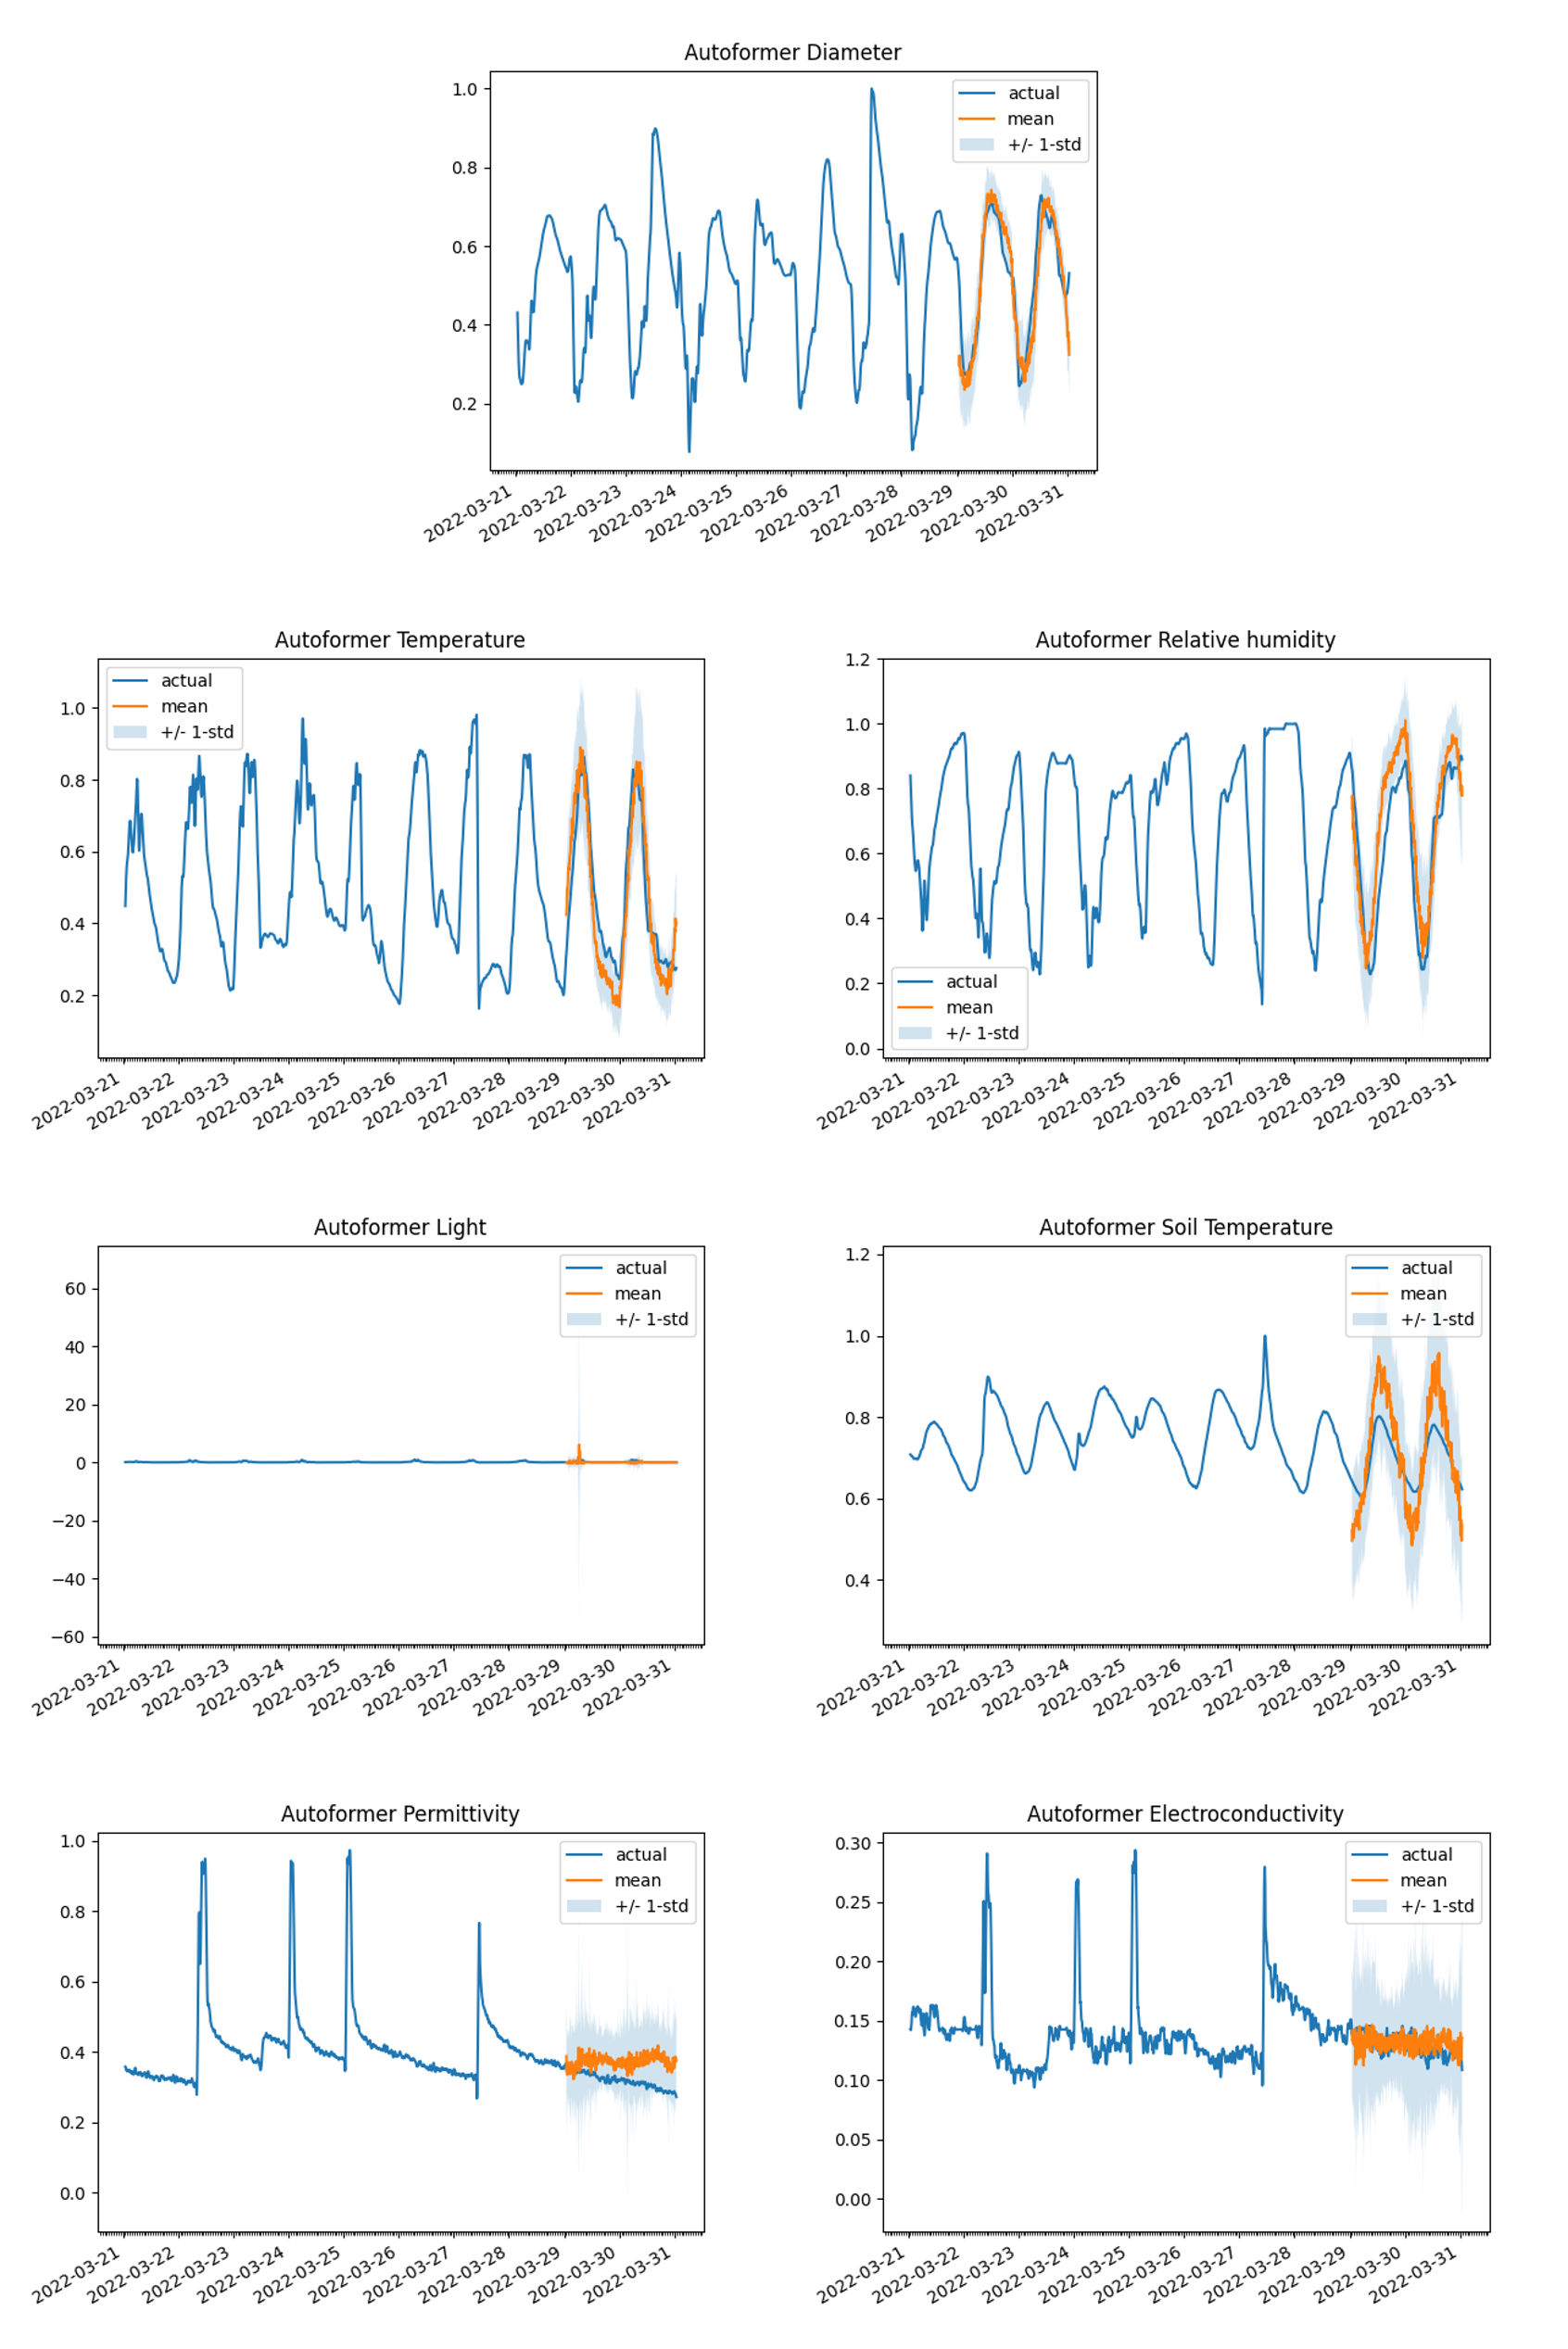
\includegraphics[width=15 cm]{6_ChapterResults/figuras/A11.png}
    \caption{Comparison between the predicted values generated by the A11 model and the actual observed values for the 7 variables over a two-day prediction horizon}
    \label{A11}
\end{figure}

\section{Results Changing the Dropout}
In this section, we examine the results of experiments that involved varying the Dropout rates across different models. Dropout is a regularization technique used to prevent overfitting by randomly dropping units during training, and its impact on model performance can be significant. By adjusting Dropout rates, we aim to understand how this parameter influences the models' ability to generalize, specifically in terms of their predictive accuracy and stability.

\subsection{Transformer}
The results for the Transformer variant with modified Dropout values, as shown in Tables \ref{T3_M} and \ref{T3_R}, indicate mixed performance compared to the T13 model, which served as the baseline for this experimental phase. While these models underperform in predicting the plant diameter, they show improvement in forecasting the other environmental variables. Due to this enhanced ability to predict a broader range of variables, Model T15 is considered the best model in this phase. Figure \ref{T15} presents a side-by-side comparison of the T15 model's predictions against the actual values, showcasing the model's predictive accuracy.

Additionally, as seen in \ref{T3_T}, adjusting the Dropout values has minimal impact on training times, with little to no variation observed.


\begin{table}[]
    \centering
    \resizebox{\textwidth}{!}{%
    \begin{tabular}{ccccccccc}
    \multicolumn{9}{c}{\textbf{MSE   (Sorted by model)}}                                                                                                                                                                                                                          \\
    Model & Diameter                       & Electroconductivity            & Light                          & Permittivity                   & Relative Humidity              & Soil Temperature               & Temperature                    & Mean                           \\
    T14   & \cellcolor[HTML]{F8696B}-19.46 & \cellcolor[HTML]{F8696B}-23.07 & \cellcolor[HTML]{FFEB84}-14.03 & \cellcolor[HTML]{F8696B}-5.46  & \cellcolor[HTML]{63BE7B}-19.15 & \cellcolor[HTML]{F8696B}-12.16 & \cellcolor[HTML]{63BE7B}-20.31 & \cellcolor[HTML]{F8696B}-16.23 \\
    T15   & \cellcolor[HTML]{63BE7B}-20.48 & \cellcolor[HTML]{FFEB84}-30.30 & \cellcolor[HTML]{63BE7B}-14.25 & \cellcolor[HTML]{63BE7B}-34.57 & \cellcolor[HTML]{FFEB84}-15.44 & \cellcolor[HTML]{63BE7B}-23.28 & \cellcolor[HTML]{FFEB84}-17.85 & \cellcolor[HTML]{63BE7B}-22.31 \\
    T16   & \cellcolor[HTML]{FFEB84}-19.75 & \cellcolor[HTML]{63BE7B}-37.64 & \cellcolor[HTML]{F8696B}-13.06 & \cellcolor[HTML]{FFEB84}-24.54 & \cellcolor[HTML]{F8696B}-8.32  & \cellcolor[HTML]{FFEB84}-12.23 & \cellcolor[HTML]{F8696B}-16.79 & \cellcolor[HTML]{FFEB84}-18.91
    \end{tabular}%
    }
    \caption{Mean Squared Errors (MSE) for different Transformer models obtained by varying the Dropout, sorted by model}
    \label{T3_M}
    \end{table}


\begin{table}[]
    \centering
    \resizebox{\textwidth}{!}{%
    \begin{tabular}{ccccccccc}
    \multicolumn{9}{c}{\textbf{R2 (Sorted by model)}}                                                                                                                                                                                                                       \\
    Model & Diameter                     & Electroconductivity            & Light                        & Permittivity                    & Relative\_humidity            & Soil\_Temperature              & Temperature                  & Mean                           \\
    T14   & \cellcolor[HTML]{F8696B}0.49 & \cellcolor[HTML]{F8696B}-59.79 & \cellcolor[HTML]{FFEB84}0.31 & \cellcolor[HTML]{F8696B}-620.24 & \cellcolor[HTML]{63BE7B}0.76  & \cellcolor[HTML]{F8696B}-15.16 & \cellcolor[HTML]{63BE7B}0.76 & \cellcolor[HTML]{F8696B}-98.98 \\
    T15   & \cellcolor[HTML]{63BE7B}0.60 & \cellcolor[HTML]{FFEB84}-10.51 & \cellcolor[HTML]{63BE7B}0.34 & \cellcolor[HTML]{63BE7B}0.24    & \cellcolor[HTML]{FFEB84}0.44  & \cellcolor[HTML]{63BE7B}-0.25  & \cellcolor[HTML]{FFEB84}0.58 & \cellcolor[HTML]{63BE7B}-1.22  \\
    T16   & \cellcolor[HTML]{FFEB84}0.52 & \cellcolor[HTML]{63BE7B}-1.12  & \cellcolor[HTML]{F8696B}0.14 & \cellcolor[HTML]{FFEB84}-6.68   & \cellcolor[HTML]{F8696B}-1.91 & \cellcolor[HTML]{FFEB84}-14.90 & \cellcolor[HTML]{F8696B}0.47 & \cellcolor[HTML]{FFEB84}-3.36 
    \end{tabular}%
    }
    \caption{R-squared (R²) for different Transformer models obtained by varying the Dropout, sorted by model}
    \label{T3_R}
    \end{table}



\begin{table}[]
    \begin{tabular}{cc}
    \multicolumn{2}{c}{\textbf{Training   Time (Sorted by model)}} \\
    Model             & Training time {[}s{]}                      \\
    T14               & \cellcolor[HTML]{63BE7B}252.21             \\
    T15               & \cellcolor[HTML]{FFEB84}257.21             \\
    T16               & \cellcolor[HTML]{F8696B}258.09            
    \end{tabular}
    \caption{Training times for different Transformer models obtained by varying the Dropout, sorted by model}
    \label{T3_T}
    \end{table}

\begin{figure}[htbp]
    \centering
    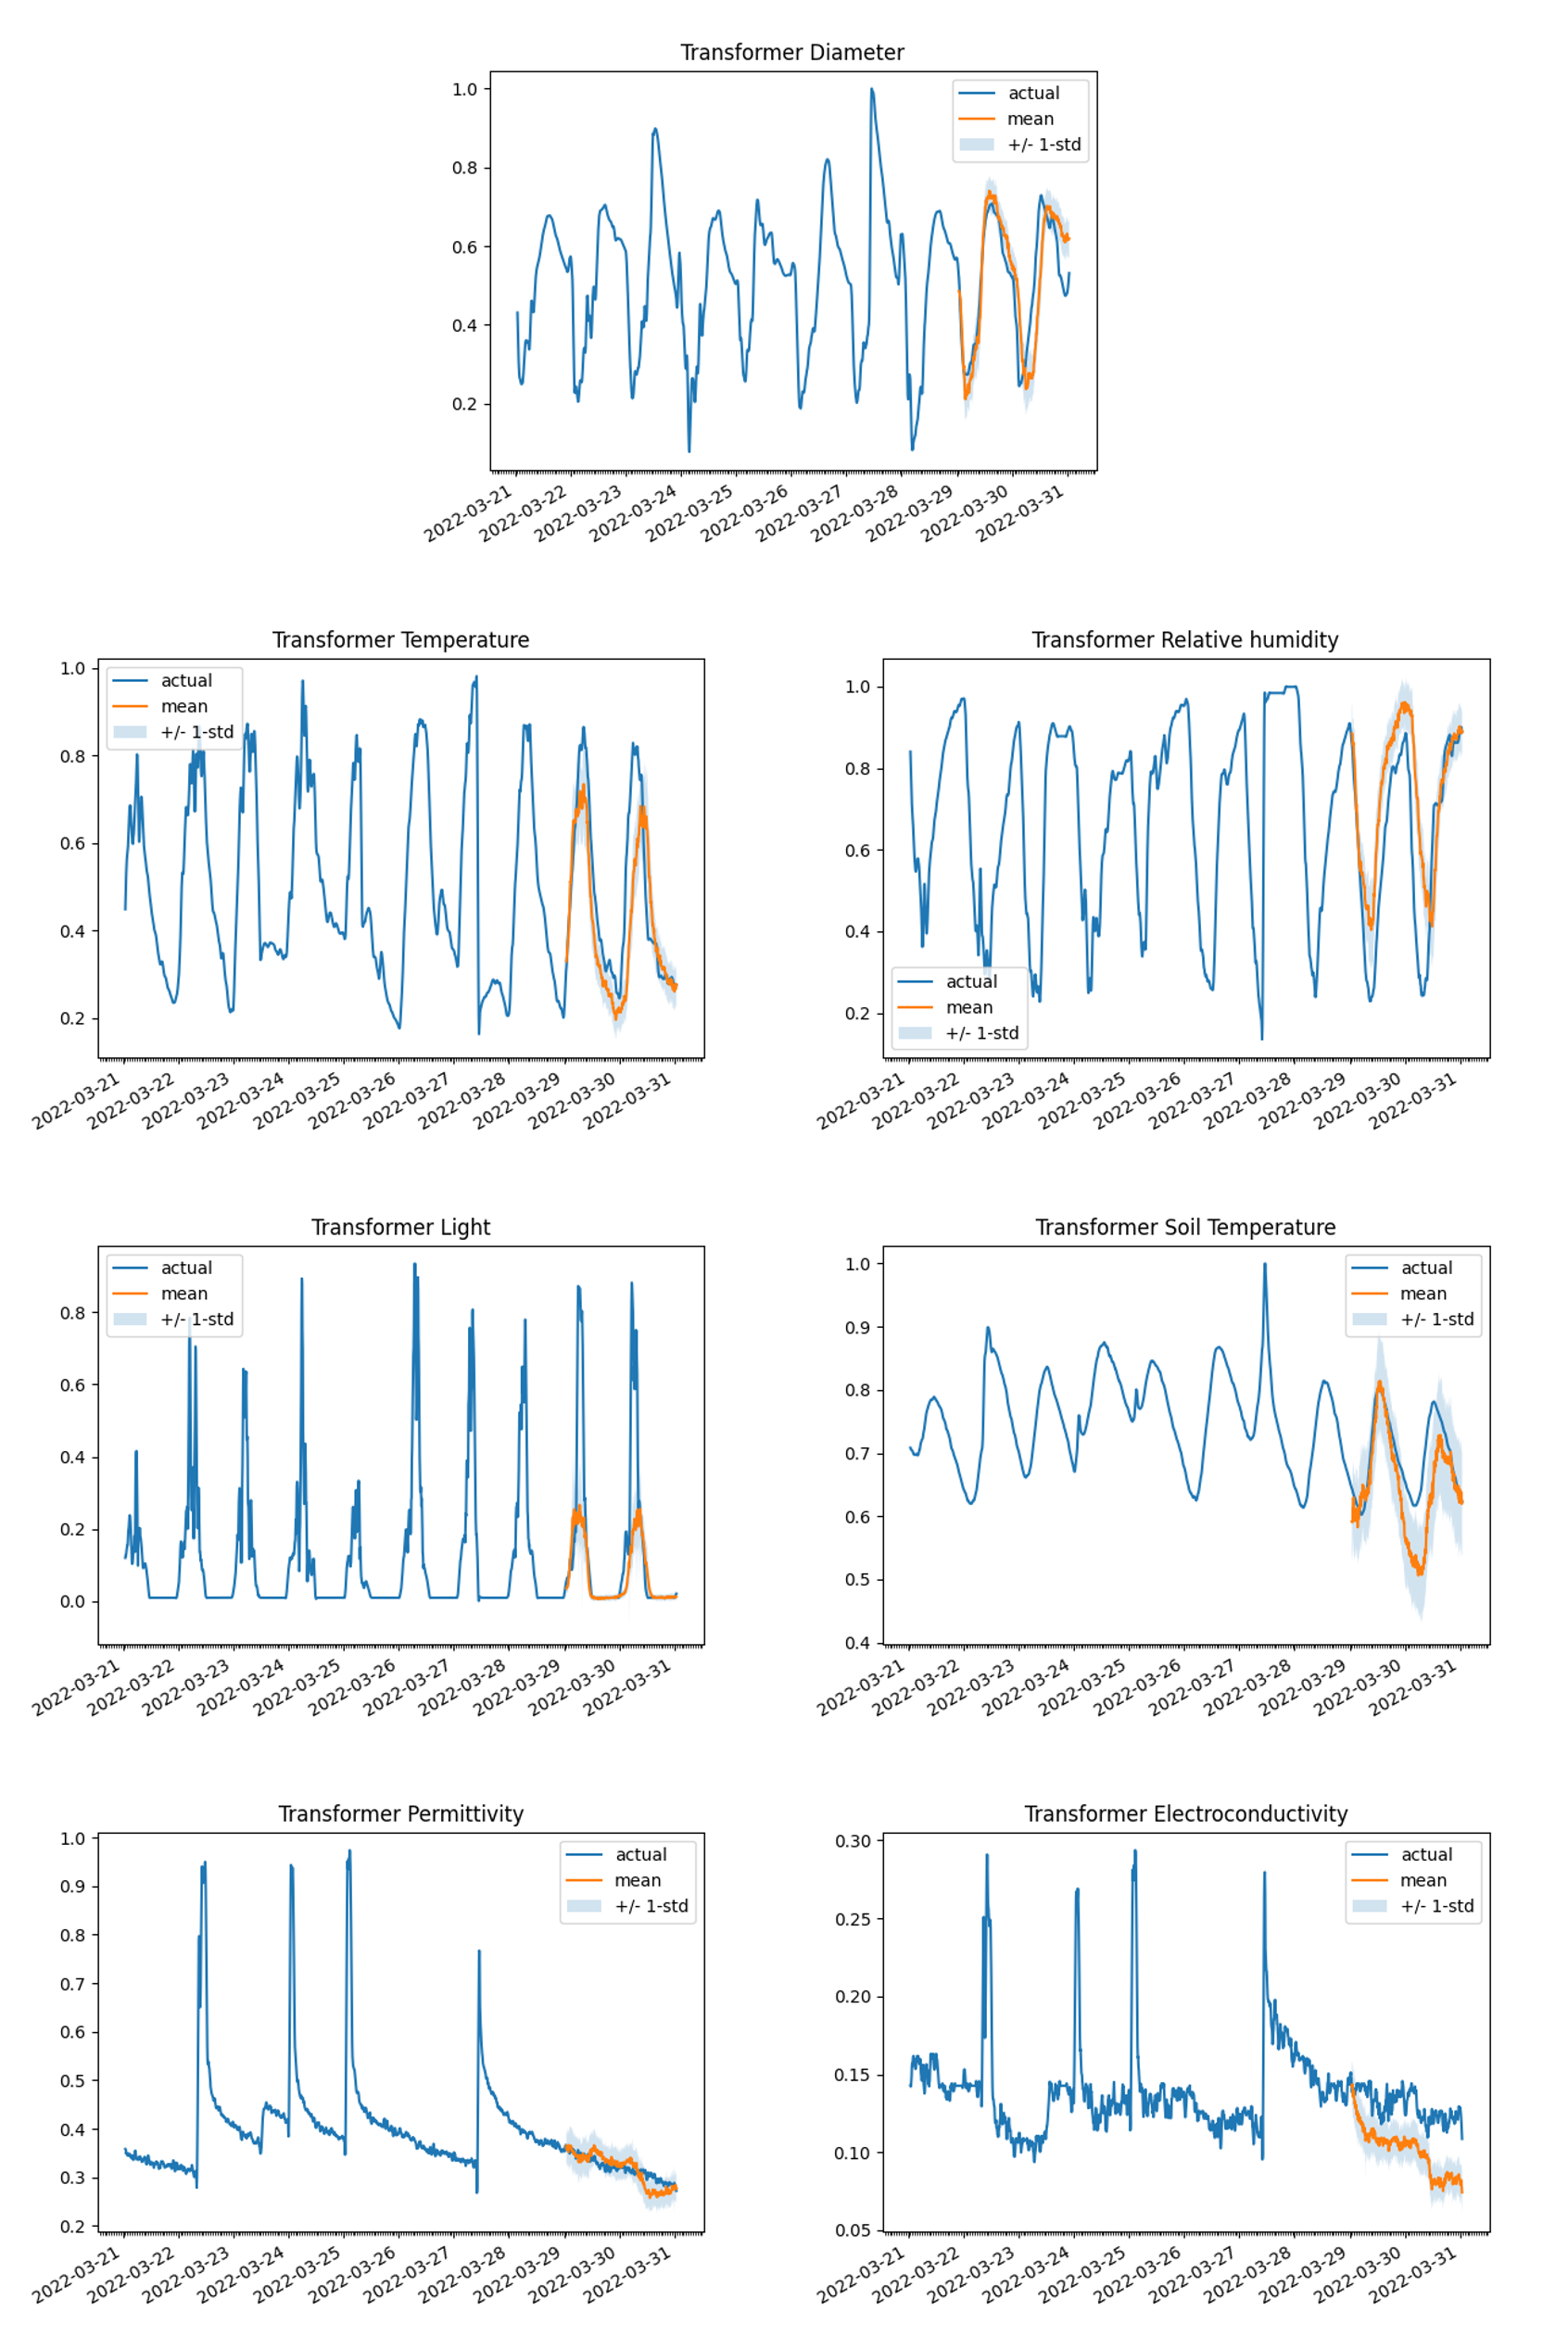
\includegraphics[width=15 cm]{6_ChapterResults/figuras/T15.png}
    \caption{Comparison between the predicted values generated by the T15 model and the actual observed values for the 7 variables over a two-day prediction horizon}
    \label{T15}
\end{figure}

\subsection{Informer}
The results for the Informer variant with modified Dropout values, as shown in Tables \ref{I3_M} and \ref{I3_R}, reveal slight improvements in predicting plant diameter compared to the I13 model, which served as the baseline for this experimental phase. However, these models perform slightly worse when predicting other environmental variables. As a result, I13 remains the best model obtained so far.

Additionally, as seen in Table \ref{I3_T}, training times increase slightly with changes in Dropout values, but the impact on computational efficiency is minimal.


\begin{table}[]
    \centering
    \resizebox{\textwidth}{!}{%
    \begin{tabular}{ccccccccc}
    \multicolumn{9}{c}{\textbf{MSE   (Sorted by model)}}                                                                                                                                                                                                                          \\
    Model & Diameter                       & Electroconductivity            & Light                          & Permittivity                   & Relative\_humidity             & Soil\_Temperature              & Temperature                    & Mean                           \\
    I14   & \cellcolor[HTML]{F8696B}-18.29 & \cellcolor[HTML]{FFEB84}-28.35 & \cellcolor[HTML]{F8696B}-12.21 & \cellcolor[HTML]{F8696B}-24.76 & \cellcolor[HTML]{63BE7B}-11.89 & \cellcolor[HTML]{FFEB84}-9.29  & \cellcolor[HTML]{FFEB84}-13.23 & \cellcolor[HTML]{F8696B}-16.86 \\
    I15   & \cellcolor[HTML]{FFEB84}-22.29 & \cellcolor[HTML]{63BE7B}-33.13 & \cellcolor[HTML]{FFEB84}-12.63 & \cellcolor[HTML]{63BE7B}-29.98 & \cellcolor[HTML]{FFEB84}-11.37 & \cellcolor[HTML]{F8696B}-8.38  & \cellcolor[HTML]{F8696B}-11.97 & \cellcolor[HTML]{63BE7B}-18.54 \\
    I16   & \cellcolor[HTML]{63BE7B}-22.99 & \cellcolor[HTML]{F8696B}-25.84 & \cellcolor[HTML]{63BE7B}-12.76 & \cellcolor[HTML]{FFEB84}-24.76 & \cellcolor[HTML]{F8696B}-9.70  & \cellcolor[HTML]{63BE7B}-10.53 & \cellcolor[HTML]{63BE7B}-13.48 & \cellcolor[HTML]{FFEB84}-17.15
    \end{tabular}%
    }
    \caption{Mean Squared Errors (MSE) for different Informer models obtained by varying the Dropout, sorted by model}
    \label{I3_M}
    \end{table}

\begin{table}[]
    \centering
    \resizebox{\textwidth}{!}{%
    \begin{tabular}{ccccccccc}
    \multicolumn{9}{c}{\textbf{R2 (Sorted by model)}}                                                                                                                                                                                                                      \\
    Model & Diameter                     & Electroconductivity            & Light                         & Permittivity                  & Relative\_humidity            & Soil\_Temperature              & Temperature                   & Mean                          \\
    I14   & \cellcolor[HTML]{F8696B}0.33 & \cellcolor[HTML]{FFEB84}-17.00 & \cellcolor[HTML]{F8696B}-0.05 & \cellcolor[HTML]{F8696B}-6.30 & \cellcolor[HTML]{63BE7B}-0.28 & \cellcolor[HTML]{FFEB84}-30.30 & \cellcolor[HTML]{FFEB84}-0.21 & \cellcolor[HTML]{FFEB84}-7.69 \\
    I15   & \cellcolor[HTML]{FFEB84}0.73 & \cellcolor[HTML]{63BE7B}-4.99  & \cellcolor[HTML]{FFEB84}0.05  & \cellcolor[HTML]{63BE7B}-1.19 & \cellcolor[HTML]{FFEB84}-0.44 & \cellcolor[HTML]{F8696B}-37.60 & \cellcolor[HTML]{F8696B}-0.62 & \cellcolor[HTML]{63BE7B}-6.29 \\
    I16   & \cellcolor[HTML]{63BE7B}0.77 & \cellcolor[HTML]{F8696B}-31.09 & \cellcolor[HTML]{63BE7B}0.07  & \cellcolor[HTML]{FFEB84}-6.30 & \cellcolor[HTML]{F8696B}-1.12 & \cellcolor[HTML]{63BE7B}-22.52 & \cellcolor[HTML]{63BE7B}-0.14 & \cellcolor[HTML]{F8696B}-8.62
    \end{tabular}%
    }
    \caption{R-squared (R²) for different Informer models obtained by varying the Dropout, sorted by model}
    \label{I3_R}
    \end{table}


\begin{table}[]
    \begin{tabular}{cc}
    \multicolumn{2}{c}{\textbf{Training   Time (Sorted by model)}} \\
    Model             & Training time {[}s{]}                      \\
    I14               & \cellcolor[HTML]{63BE7B}140.69             \\
    I15               & \cellcolor[HTML]{FFEB84}142.24             \\
    I16               & \cellcolor[HTML]{F8696B}145.03            
    \end{tabular}
    \caption{Training times for different Informer models obtained by varying the Dropout, sorted by model}
    \label{I3_T}
    \end{table}


\subsection{Autoformer}
The results for the Autoformer variant with modified Dropout values, as shown in Tables \ref{A3_M} and \ref{A3_R}, indicate varied outcomes compared to the A11 model, which served as the baseline for this experimental phase. While specific details about performance changes are not provided, the variations in Dropout likely influenced the model's ability to generalize and prevent overfitting.

Additionally, as seen in Table \ref{A3_T}, training times were reduced when Dropout was applied. This reduction in training time suggests that the model may have been more efficient during training, likely due to the regularization effect of Dropout, which reduces the complexity of the model during the learning process.


\begin{table}[]
    \centering
    \resizebox{\textwidth}{!}{%
    \begin{tabular}{ccccccccc}
    \multicolumn{9}{c}{\textbf{MSE   (Sorted by model)}}                                                                                                                                                                                                                          \\
    Model & Diameter                       & Electroconductivity            & Light                          & Permittivity                   & Relative\_humidity             & Soil\_Temperature              & Temperature                    & Mean                           \\
    A14   & \cellcolor[HTML]{63BE7B}-25.21 & \cellcolor[HTML]{F8696B}-37.91 & \cellcolor[HTML]{FFEB84}-11.47 & \cellcolor[HTML]{F8696B}-23.76 & \cellcolor[HTML]{63BE7B}-20.63 & \cellcolor[HTML]{63BE7B}-18.92 & \cellcolor[HTML]{63BE7B}-23.66 & \cellcolor[HTML]{63BE7B}-23.08 \\
    A15   & \cellcolor[HTML]{FFEB84}-20.46 & \cellcolor[HTML]{FFEB84}-38.95 & \cellcolor[HTML]{63BE7B}-11.67 & \cellcolor[HTML]{FFEB84}-24.51 & \cellcolor[HTML]{FFEB84}-15.36 & \cellcolor[HTML]{F8696B}-16.75 & \cellcolor[HTML]{FFEB84}-20.50 & \cellcolor[HTML]{FFEB84}-21.17 \\
    A16   & \cellcolor[HTML]{F8696B}-18.64 & \cellcolor[HTML]{63BE7B}-39.43 & \cellcolor[HTML]{F8696B}-11.18 & \cellcolor[HTML]{63BE7B}-27.39 & \cellcolor[HTML]{F8696B}-14.12 & \cellcolor[HTML]{FFEB84}-18.22 & \cellcolor[HTML]{F8696B}-16.85 & \cellcolor[HTML]{F8696B}-20.83
    \end{tabular}%
    }
    \caption{Mean Squared Errors (MSE) for different Autoformer models obtained by varying the Dropout, sorted by model}
    \label{A3_M}
    \end{table}


\begin{table}[]
    \centering
    \resizebox{\textwidth}{!}{%
    \begin{tabular}{ccccccccc}
    \multicolumn{9}{c}{\textbf{R2 (Sorted by model)}}                                                                                                                                                                                                                  \\
    Model & Diameter                     & Electroconductivity           & Light                         & Permittivity                  & Relative\_humidity           & Soil\_Temperature             & Temperature                  & Mean                          \\
    A14   & \cellcolor[HTML]{63BE7B}0.86 & \cellcolor[HTML]{F8696B}-0.99 & \cellcolor[HTML]{FFEB84}-0.25 & \cellcolor[HTML]{F8696B}-8.20 & \cellcolor[HTML]{63BE7B}0.83 & \cellcolor[HTML]{63BE7B}-2.41 & \cellcolor[HTML]{63BE7B}0.89 & \cellcolor[HTML]{FFEB84}-1.32 \\
    A15   & \cellcolor[HTML]{FFEB84}0.59 & \cellcolor[HTML]{FFEB84}-0.57 & \cellcolor[HTML]{63BE7B}-0.19 & \cellcolor[HTML]{FFEB84}-6.72 & \cellcolor[HTML]{FFEB84}0.42 & \cellcolor[HTML]{F8696B}-4.62 & \cellcolor[HTML]{FFEB84}0.77 & \cellcolor[HTML]{F8696B}-1.47 \\
    A16   & \cellcolor[HTML]{F8696B}0.38 & \cellcolor[HTML]{63BE7B}-0.41 & \cellcolor[HTML]{F8696B}-0.33 & \cellcolor[HTML]{63BE7B}-2.98 & \cellcolor[HTML]{F8696B}0.24 & \cellcolor[HTML]{FFEB84}-3.00 & \cellcolor[HTML]{F8696B}0.47 & \cellcolor[HTML]{63BE7B}-0.80
    \end{tabular}%
    }
    \caption{R-squared (R²) for different Autoformer models obtained by varying the Dropout, sorted by model}
    \label{A3_R}
    \end{table}


\begin{table}[]
    \begin{tabular}{cc}
    \multicolumn{2}{c}{\textbf{Training   Time (Sorted by model)}} \\
    Model             & Training time {[}s{]}                      \\
    A14               & \cellcolor[HTML]{F8696B}308.12             \\
    A15               & \cellcolor[HTML]{FFEB84}304.43             \\
    A16               & \cellcolor[HTML]{63BE7B}298.24            
    \end{tabular}
    \caption{Training times for different Autoformer models obtained by varying the Dropout, sorted by model}
    \label{A3_T}
    \end{table}

\section{Results Changing the Encoder Layers, Decoder Layers, and Dimensionality of the Transformer Layers}

In this section, we present the results of experiments involving changes to the Encoder Layers, Decoder Layers, and Dimensionality of the Transformer Layers across various model variants. This phase of experimentation aims to explore how modifications in these architectural parameters impact the performance of the Transformer, Informer, and Autoformer models. By systematically adjusting these key aspects of the model architecture, we seek to identify configurations that optimize predictive accuracy while balancing computational efficiency.

\subsection{Transformer}
The results for the Transformer variant with modified Encoder Layers, Decoder Layers, and Dimensionality, as shown in Tables \ref{T4_M} and \ref{T4_R}, exhibit mixed performance compared to the T15 model, which served as the baseline for this phase of experimentation. Some models showed better results in specific variables, while others performed worse. These variations can be attributed to changes in model complexity. On one hand, adding layers or increasing dimensionality can enhance the model's ability to capture complex patterns; on the other hand, it can also lead to overfitting or increased difficulty in effective training. However, none of these models significantly outperformed the existing ones, and as a result, T15 remains the best model among those tested.

Additionally, as seen in Table \ref{T4_T}, increasing the number of layers leads to higher computational costs and, consequently, longer training times.


\begin{table}[]
    \centering
    \resizebox{\textwidth}{!}{%
    \begin{tabular}{ccccccccc}
    \multicolumn{9}{c}{\textbf{MSE   (Sorted by model)}}                                                                                                                                                                                                                          \\
    Model & Diameter                       & Electroconductivity            & Light                          & Permittivity                   & Relative Humidity              & Soil Temperature               & Temperature                    & Mean                           \\
    T17   & \cellcolor[HTML]{FDB47A}-18.99 & \cellcolor[HTML]{A7D17E}-36.81 & \cellcolor[HTML]{F8696B}-12.59 & \cellcolor[HTML]{7AC47C}-27.62 & \cellcolor[HTML]{FA8E72}-10.95 & \cellcolor[HTML]{FFE182}-12.36 & \cellcolor[HTML]{FB9073}-15.53 & \cellcolor[HTML]{F0E683}-19.26 \\
    T18   & \cellcolor[HTML]{CDDC81}-21.58 & \cellcolor[HTML]{F8696B}-19.96 & \cellcolor[HTML]{FED280}-13.93 & \cellcolor[HTML]{F8696B}-9.39  & \cellcolor[HTML]{F8696B}-10.04 & \cellcolor[HTML]{F8696B}-8.74  & \cellcolor[HTML]{F0E683}-18.71 & \cellcolor[HTML]{F8696B}-14.62 \\
    T19   & \cellcolor[HTML]{E6E382}-20.99 & \cellcolor[HTML]{63BE7B}-43.19 & \cellcolor[HTML]{D9E081}-14.58 & \cellcolor[HTML]{C2D980}-23.41 & \cellcolor[HTML]{FAE983}-13.54 & \cellcolor[HTML]{9CCE7E}-21.04 & \cellcolor[HTML]{D9E081}-19.58 & \cellcolor[HTML]{63BE7B}-22.33 \\
    T20   & \cellcolor[HTML]{F8696B}-17.07 & \cellcolor[HTML]{DBE081}-31.96 & \cellcolor[HTML]{FCAC78}-13.45 & \cellcolor[HTML]{FFDC81}-18.60 & \cellcolor[HTML]{FFE283}-13.08 & \cellcolor[HTML]{FBE983}-13.01 & \cellcolor[HTML]{F8696B}-14.41 & \cellcolor[HTML]{FDBC7B}-17.37 \\
    T21   & \cellcolor[HTML]{63BE7B}-24.14 & \cellcolor[HTML]{FCA577}-23.93 & \cellcolor[HTML]{63BE7B}-15.60 & \cellcolor[HTML]{E9E482}-21.13 & \cellcolor[HTML]{63BE7B}-21.40 & \cellcolor[HTML]{FECF7F}-11.83 & \cellcolor[HTML]{63BE7B}-23.90 & \cellcolor[HTML]{C1D980}-20.28 \\
    T22   & \cellcolor[HTML]{FDEA83}-20.43 & \cellcolor[HTML]{91CB7D}-38.85 & \cellcolor[HTML]{FB9574}-13.14 & \cellcolor[HTML]{63BE7B}-29.00 & \cellcolor[HTML]{FDB87B}-12.01 & \cellcolor[HTML]{89C97D}-22.70 & \cellcolor[HTML]{EFE683}-18.75 & \cellcolor[HTML]{6CC07B}-22.13 \\
    T23   & \cellcolor[HTML]{FFDD82}-20.03 & \cellcolor[HTML]{FDB97B}-25.21 & \cellcolor[HTML]{D6DF81}-14.61 & \cellcolor[HTML]{FB9674}-12.95 & \cellcolor[HTML]{8CC97D}-19.25 & \cellcolor[HTML]{FA8671}-9.61  & \cellcolor[HTML]{FCAA78}-16.29 & \cellcolor[HTML]{FCAC78}-16.85 \\
    T24   & \cellcolor[HTML]{FFEA84}-20.38 & \cellcolor[HTML]{FB9C75}-23.34 & \cellcolor[HTML]{C7DB80}-14.73 & \cellcolor[HTML]{FCA978}-14.51 & \cellcolor[HTML]{F5E883}-13.79 & \cellcolor[HTML]{63BE7B}-25.97 & \cellcolor[HTML]{FFDA81}-17.68 & \cellcolor[HTML]{FFE283}-18.63
    \end{tabular}%
    }
    \caption{Mean Squared Errors (MSE) for different Transformer models obtained by varying the number of Encoder Layers, Decoder Layers, and Dimensionality of the Transformer Layers, sorted by model}
    \label{T4_M}
    \end{table}

\begin{table}[]
    \centering
    \resizebox{\textwidth}{!}{%
    \begin{tabular}{ccccccccc}
    \multicolumn{9}{c}{\textbf{R2 (Sorted by model)}}                                                                                                                                                                                                                        \\
    Model & Diameter                     & Electroconductivity             & Light                        & Permittivity                    & Relative\_humidity            & Soil\_Temperature              & Temperature                  & Mean                           \\
    T17   & \cellcolor[HTML]{FCBF7B}0.43 & \cellcolor[HTML]{72C37C}-1.57   & \cellcolor[HTML]{F8696B}0.04 & \cellcolor[HTML]{6BC17C}-2.77   & \cellcolor[HTML]{FA9773}-0.59 & \cellcolor[HTML]{FEE482}-14.46 & \cellcolor[HTML]{FA9C74}0.29 & \cellcolor[HTML]{8FCB7E}-2.66  \\
    T18   & \cellcolor[HTML]{BFD981}0.69 & \cellcolor[HTML]{F8696B}-123.50 & \cellcolor[HTML]{FDD680}0.29 & \cellcolor[HTML]{F8696B}-250.10 & \cellcolor[HTML]{F8696B}-0.96 & \cellcolor[HTML]{F8696B}-34.52 & \cellcolor[HTML]{E6E483}0.66 & \cellcolor[HTML]{F8696B}-58.21 \\
    T19   & \cellcolor[HTML]{DEE283}0.64 & \cellcolor[HTML]{63BE7B}0.41    & \cellcolor[HTML]{D5DF82}0.39 & \cellcolor[HTML]{9ACE7F}-8.95   & \cellcolor[HTML]{F6E984}0.12  & \cellcolor[HTML]{74C37C}-1.09  & \cellcolor[HTML]{C4DA81}0.72 & \cellcolor[HTML]{73C37C}-1.11  \\
    T20   & \cellcolor[HTML]{F8696B}0.12 & \cellcolor[HTML]{97CD7E}-6.85   & \cellcolor[HTML]{FBB279}0.21 & \cellcolor[HTML]{FEE783}-29.17  & \cellcolor[HTML]{FEE482}0.03  & \cellcolor[HTML]{F3E884}-12.29 & \cellcolor[HTML]{F8696B}0.08 & \cellcolor[HTML]{D9E082}-6.84  \\
    T21   & \cellcolor[HTML]{63BE7B}0.83 & \cellcolor[HTML]{FDC87D}-48.88  & \cellcolor[HTML]{63BE7B}0.52 & \cellcolor[HTML]{CDDD82}-15.83  & \cellcolor[HTML]{63BE7B}0.86  & \cellcolor[HTML]{FDD880}-16.43 & \cellcolor[HTML]{63BE7B}0.90 & \cellcolor[HTML]{FEE582}-11.15 \\
    T22   & \cellcolor[HTML]{FEEB84}0.59 & \cellcolor[HTML]{6BC17C}-0.61   & \cellcolor[HTML]{FA9A74}0.15 & \cellcolor[HTML]{63BE7B}-1.75   & \cellcolor[HTML]{FCC27C}-0.24 & \cellcolor[HTML]{6CC17C}-0.43  & \cellcolor[HTML]{E5E483}0.66 & \cellcolor[HTML]{63BE7B}-0.23  \\
    T23   & \cellcolor[HTML]{FEE082}0.55 & \cellcolor[HTML]{FDD880}-36.09  & \cellcolor[HTML]{D1DE82}0.40 & \cellcolor[HTML]{FCB97A}-109.74 & \cellcolor[HTML]{76C47D}0.77  & \cellcolor[HTML]{FA9072}-28.06 & \cellcolor[HTML]{FCB77A}0.40 & \cellcolor[HTML]{FCC17C}-24.54 \\
    T24   & \cellcolor[HTML]{FEEA83}0.59 & \cellcolor[HTML]{FCBE7B}-56.16  & \cellcolor[HTML]{C2DA81}0.41 & \cellcolor[HTML]{FDCC7E}-76.37  & \cellcolor[HTML]{ECE683}0.17  & \cellcolor[HTML]{63BE7B}0.33   & \cellcolor[HTML]{FEDF81}0.56 & \cellcolor[HTML]{FDD17F}-18.64
    \end{tabular}%
    }
    \caption{R-squared (R²) for different Transformer models obtained by varying the number of Encoder Layers, Decoder Layers, and Dimensionality of the Transformer Layers, sorted by model}
    \label{T4_R}
    \end{table}



\begin{table}[]
    \begin{tabular}{ccccc}
    \multicolumn{2}{c}{\textbf{Training   Time (Sorted by model)}} &  & \multicolumn{2}{c}{\textbf{Training Time (Sorted   by model)}} \\
    Model             & Training time {[}s{]}                      &  & Model             & Training time {[}s{]}                      \\
    T17               & \cellcolor[HTML]{63BE7B}143.56             &  & T17               & \cellcolor[HTML]{63BE7B}143.56             \\
    T18               & \cellcolor[HTML]{A8D17E}197.91             &  & T18               & \cellcolor[HTML]{A8D17E}197.91             \\
    T19               & \cellcolor[HTML]{FFE483}275.11             &  & T20               & \cellcolor[HTML]{A8D17E}198.02             \\
    T20               & \cellcolor[HTML]{A8D17E}198.02             &  & T22               & \cellcolor[HTML]{F3E783}257.47             \\
    T21               & \cellcolor[HTML]{FBA176}351.72             &  & T19               & \cellcolor[HTML]{FFE483}275.11             \\
    T22               & \cellcolor[HTML]{F3E783}257.47             &  & T23               & \cellcolor[HTML]{FDC17C}315.29             \\
    T23               & \cellcolor[HTML]{FDC17C}315.29             &  & T21               & \cellcolor[HTML]{FBA176}351.72             \\
    T24               & \cellcolor[HTML]{F8696B}415.78             &  & T24               & \cellcolor[HTML]{F8696B}415.78            
    \end{tabular}
    \caption{Training times for different Transformer models obtained by varying the number of Encoder Layers, Decoder Layers, and Dimensionality of the Transformer Layers, sorted by model and training time values}
    \label{T4_T}
    \end{table}


\subsection{Informer}
The results for the Informer variant with modified Encoder Layers, Decoder Layers, and Dimensionality of the Transformer Layers, as shown in Tables \ref{I4_M} and \ref{I4_R}, reveal a range of performance outcomes when compared to the I13 model, which was used as the baseline for this experimental phase. Similar to the Transformer results, the performance across these models is quite varied. Among all the models tested, I20 is considered the best due to its superior overall performance. The effectiveness of the I20 model is demonstrated in Figure \ref{I20}, where its predictions are compared with the corresponding real values.

Additionally, as seen in Table \ref{I4_T}, increasing the number of layers results in higher computational costs, just as with the Transformer models. However, when compared to the Transformer models, the Informer models remain more computationally efficient despite the increased complexity.




\begin{table}[]
    \centering
    \resizebox{\textwidth}{!}{%
    \begin{tabular}{ccccccccc}
    \multicolumn{9}{c}{\textbf{MSE   (Sorted by model)}}                                                                                                                                                                                                                          \\
    Model & Diameter                       & Electroconductivity            & Light                          & Permittivity                   & Relative\_humidity             & Soil\_Temperature              & Temperature                    & Mean                           \\
    I17   & \cellcolor[HTML]{97CD7E}-21.74 & \cellcolor[HTML]{DEE182}-29.26 & \cellcolor[HTML]{63BE7B}-13.13 & \cellcolor[HTML]{E1E282}-16.98 & \cellcolor[HTML]{63BE7B}-11.97 & \cellcolor[HTML]{E0E282}-17.31 & \cellcolor[HTML]{A7D17E}-15.57 & \cellcolor[HTML]{9FCF7E}-18.00 \\
    I18   & \cellcolor[HTML]{FFDB81}-19.94 & \cellcolor[HTML]{63BE7B}-34.20 & \cellcolor[HTML]{C9DB80}-12.68 & \cellcolor[HTML]{63BE7B}-28.54 & \cellcolor[HTML]{FFDD82}-11.06 & \cellcolor[HTML]{FCAF79}-13.65 & \cellcolor[HTML]{F9E983}-13.84 & \cellcolor[HTML]{63BE7B}-19.13 \\
    I19   & \cellcolor[HTML]{FDB97B}-18.59 & \cellcolor[HTML]{F97C6F}-23.47 & \cellcolor[HTML]{FB9F76}-11.87 & \cellcolor[HTML]{FECB7E}-13.04 & \cellcolor[HTML]{E6E382}-11.42 & \cellcolor[HTML]{D1DD81}-17.94 & \cellcolor[HTML]{FFE683}-13.60 & \cellcolor[HTML]{FDBF7C}-15.70 \\
    I20   & \cellcolor[HTML]{C0D980}-21.30 & \cellcolor[HTML]{F8696B}-22.74 & \cellcolor[HTML]{CEDD81}-12.65 & \cellcolor[HTML]{F8696B}-9.33  & \cellcolor[HTML]{D7DF81}-11.48 & \cellcolor[HTML]{C1D980}-18.62 & \cellcolor[HTML]{63BE7B}-17.01 & \cellcolor[HTML]{FFE784}-16.16 \\
    I21   & \cellcolor[HTML]{FB9F76}-17.53 & \cellcolor[HTML]{F2E783}-28.47 & \cellcolor[HTML]{F8696B}-11.46 & \cellcolor[HTML]{FA8A72}-10.58 & \cellcolor[HTML]{FFE583}-11.21 & \cellcolor[HTML]{FA8972}-12.19 & \cellcolor[HTML]{FA7F70}-11.48 & \cellcolor[HTML]{F8696B}-14.70 \\
    I22   & \cellcolor[HTML]{63BE7B}-22.32 & \cellcolor[HTML]{F9706D}-22.99 & \cellcolor[HTML]{FFDF82}-12.35 & \cellcolor[HTML]{FDBD7C}-12.49 & \cellcolor[HTML]{B7D67F}-11.61 & \cellcolor[HTML]{63BE7B}-22.68 & \cellcolor[HTML]{A4D07E}-15.63 & \cellcolor[HTML]{CCDC81}-17.15 \\
    I23   & \cellcolor[HTML]{A1D07E}-21.63 & \cellcolor[HTML]{FFDF82}-27.44 & \cellcolor[HTML]{EAE582}-12.53 & \cellcolor[HTML]{C8DB80}-19.23 & \cellcolor[HTML]{FFDE82}-11.09 & \cellcolor[HTML]{F8696B}-10.97 & \cellcolor[HTML]{F8696B}-11.03 & \cellcolor[HTML]{FBEA83}-16.28 \\
    I24   & \cellcolor[HTML]{F8696B}-15.39 & \cellcolor[HTML]{B6D67F}-30.86 & \cellcolor[HTML]{F9786E}-11.58 & \cellcolor[HTML]{F1E783}-15.46 & \cellcolor[HTML]{F8696B}-9.11  & \cellcolor[HTML]{FEC97E}-14.66 & \cellcolor[HTML]{F9736D}-11.22 & \cellcolor[HTML]{FCAB78}-15.47
    \end{tabular}%
    }
    \caption{Mean Squared Errors (MSE) for different Informer models obtained by varying the number of Encoder Layers, Decoder Layers, and Dimensionality of the Transformer Layers, sorted by model}
    \label{I4_M}
    \end{table}


    


\begin{table}[]
    \centering
    \resizebox{\textwidth}{!}{%
    \begin{tabular}{ccccccccc}
    \multicolumn{9}{c}{\textbf{R2 (Sorted by model)}}                                                                                                                                                                                                                          \\
    Model & Diameter                      & Electroconductivity            & Light                         & Permittivity                    & Relative\_humidity            & Soil\_Temperature              & Temperature                   & Mean                           \\
    I17   & \cellcolor[HTML]{90CB7E}0.70  & \cellcolor[HTML]{CADC81}-13.62 & \cellcolor[HTML]{63BE7B}0.15  & \cellcolor[HTML]{B1D580}-42.75  & \cellcolor[HTML]{63BE7B}-0.26 & \cellcolor[HTML]{C5DB81}-3.94  & \cellcolor[HTML]{99CE7F}0.29  & \cellcolor[HTML]{A2D17F}-8.49  \\
    I18   & \cellcolor[HTML]{FEE282}0.54  & \cellcolor[HTML]{63BE7B}-3.68  & \cellcolor[HTML]{C7DB81}0.06  & \cellcolor[HTML]{63BE7B}-2.05   & \cellcolor[HTML]{FEDF81}-0.55 & \cellcolor[HTML]{FCC27C}-10.47 & \cellcolor[HTML]{F8E984}-0.06 & \cellcolor[HTML]{63BE7B}-2.32  \\
    I19   & \cellcolor[HTML]{FDCA7D}0.38  & \cellcolor[HTML]{F98570}-54.40 & \cellcolor[HTML]{FBA276}-0.14 & \cellcolor[HTML]{FED980}-107.44 & \cellcolor[HTML]{E5E483}-0.43 & \cellcolor[HTML]{B3D580}-3.27  & \cellcolor[HTML]{FEE683}-0.11 & \cellcolor[HTML]{FDCF7E}-23.63 \\
    I20   & \cellcolor[HTML]{B7D780}0.67  & \cellcolor[HTML]{F8696B}-64.56 & \cellcolor[HTML]{CCDD82}0.05  & \cellcolor[HTML]{F8696B}-253.73 & \cellcolor[HTML]{D5DF82}-0.41 & \cellcolor[HTML]{A2D07F}-2.65  & \cellcolor[HTML]{63BE7B}0.49  & \cellcolor[HTML]{F8696B}-45.73 \\
    I21   & \cellcolor[HTML]{FBB178}0.20  & \cellcolor[HTML]{E8E583}-16.54 & \cellcolor[HTML]{F8696B}-0.25 & \cellcolor[HTML]{FA9974}-190.27 & \cellcolor[HTML]{FEE683}-0.50 & \cellcolor[HTML]{FA9874}-15.06 & \cellcolor[HTML]{F98470}-0.82 & \cellcolor[HTML]{FBA877}-31.89 \\
    I22   & \cellcolor[HTML]{63BE7B}0.74  & \cellcolor[HTML]{F8736C}-60.91 & \cellcolor[HTML]{FEE081}-0.02 & \cellcolor[HTML]{FDCE7E}-121.98 & \cellcolor[HTML]{B5D680}-0.36 & \cellcolor[HTML]{63BE7B}-0.43  & \cellcolor[HTML]{97CD7E}0.30  & \cellcolor[HTML]{FCC37C}-26.09 \\
    I23   & \cellcolor[HTML]{9ACE7F}0.69  & \cellcolor[HTML]{FEE482}-21.21 & \cellcolor[HTML]{E9E583}0.03  & \cellcolor[HTML]{8FCB7E}-25.07  & \cellcolor[HTML]{FEE082}-0.54 & \cellcolor[HTML]{F8696B}-20.26 & \cellcolor[HTML]{F8696B}-1.01 & \cellcolor[HTML]{AED480}-9.63  \\
    I24   & \cellcolor[HTML]{F8696B}-0.31 & \cellcolor[HTML]{9BCF7F}-9.11  & \cellcolor[HTML]{F8796E}-0.22 & \cellcolor[HTML]{D3DF82}-61.05  & \cellcolor[HTML]{F8696B}-1.43 & \cellcolor[HTML]{FDD880}-8.09  & \cellcolor[HTML]{F8756D}-0.93 & \cellcolor[HTML]{C2DA81}-11.59
    \end{tabular}%
    }
    \caption{R-squared (R²) for different Informer models obtained by varying the number of Encoder Layers, Decoder Layers, and Dimensionality of the Transformer Layers, sorted by model}
    \label{I4_R}
    \end{table}



    

\begin{table}[]
    \begin{tabular}{ccccc}
    \multicolumn{2}{c}{\textbf{Training   Time (Sorted by model)}} &  & \multicolumn{2}{c}{\textbf{Training Time (Sorted   by training time)}} \\
    Model             & Training time {[}s{]}                      &  & Model                 & Training time {[}s{]}                          \\
    I17               & \cellcolor[HTML]{63BE7B}102.57             &  & I17                   & \cellcolor[HTML]{63BE7B}102.57                 \\
    I18               & \cellcolor[HTML]{E1E282}138.04             &  & I20                   & \cellcolor[HTML]{A9D27F}122.21                 \\
    I19               & \cellcolor[HTML]{F9776E}191.89             &  & I22                   & \cellcolor[HTML]{C0D980}128.8                  \\
    I20               & \cellcolor[HTML]{A9D27F}122.21             &  & I18                   & \cellcolor[HTML]{E1E282}138.04                 \\
    I21               & \cellcolor[HTML]{FA7D6F}189.34             &  & I23                   & \cellcolor[HTML]{FED781}154.3                  \\
    I22               & \cellcolor[HTML]{C0D980}128.8              &  & I21                   & \cellcolor[HTML]{FA7D6F}189.34                 \\
    I23               & \cellcolor[HTML]{FED781}154.3              &  & I19                   & \cellcolor[HTML]{F9776E}191.89                 \\
    I24               & \cellcolor[HTML]{F8696B}196.99             &  & I24                   & \cellcolor[HTML]{F8696B}196.99                
    \end{tabular}
    \caption{Training times for different Informer models obtained by varying the number of Encoder Layers, Decoder Layers, and Dimensionality of the Transformer Layers, sorted by model and training time values}
    \label{I4_T}
    \end{table}

\begin{figure}[htbp]
    \centering
    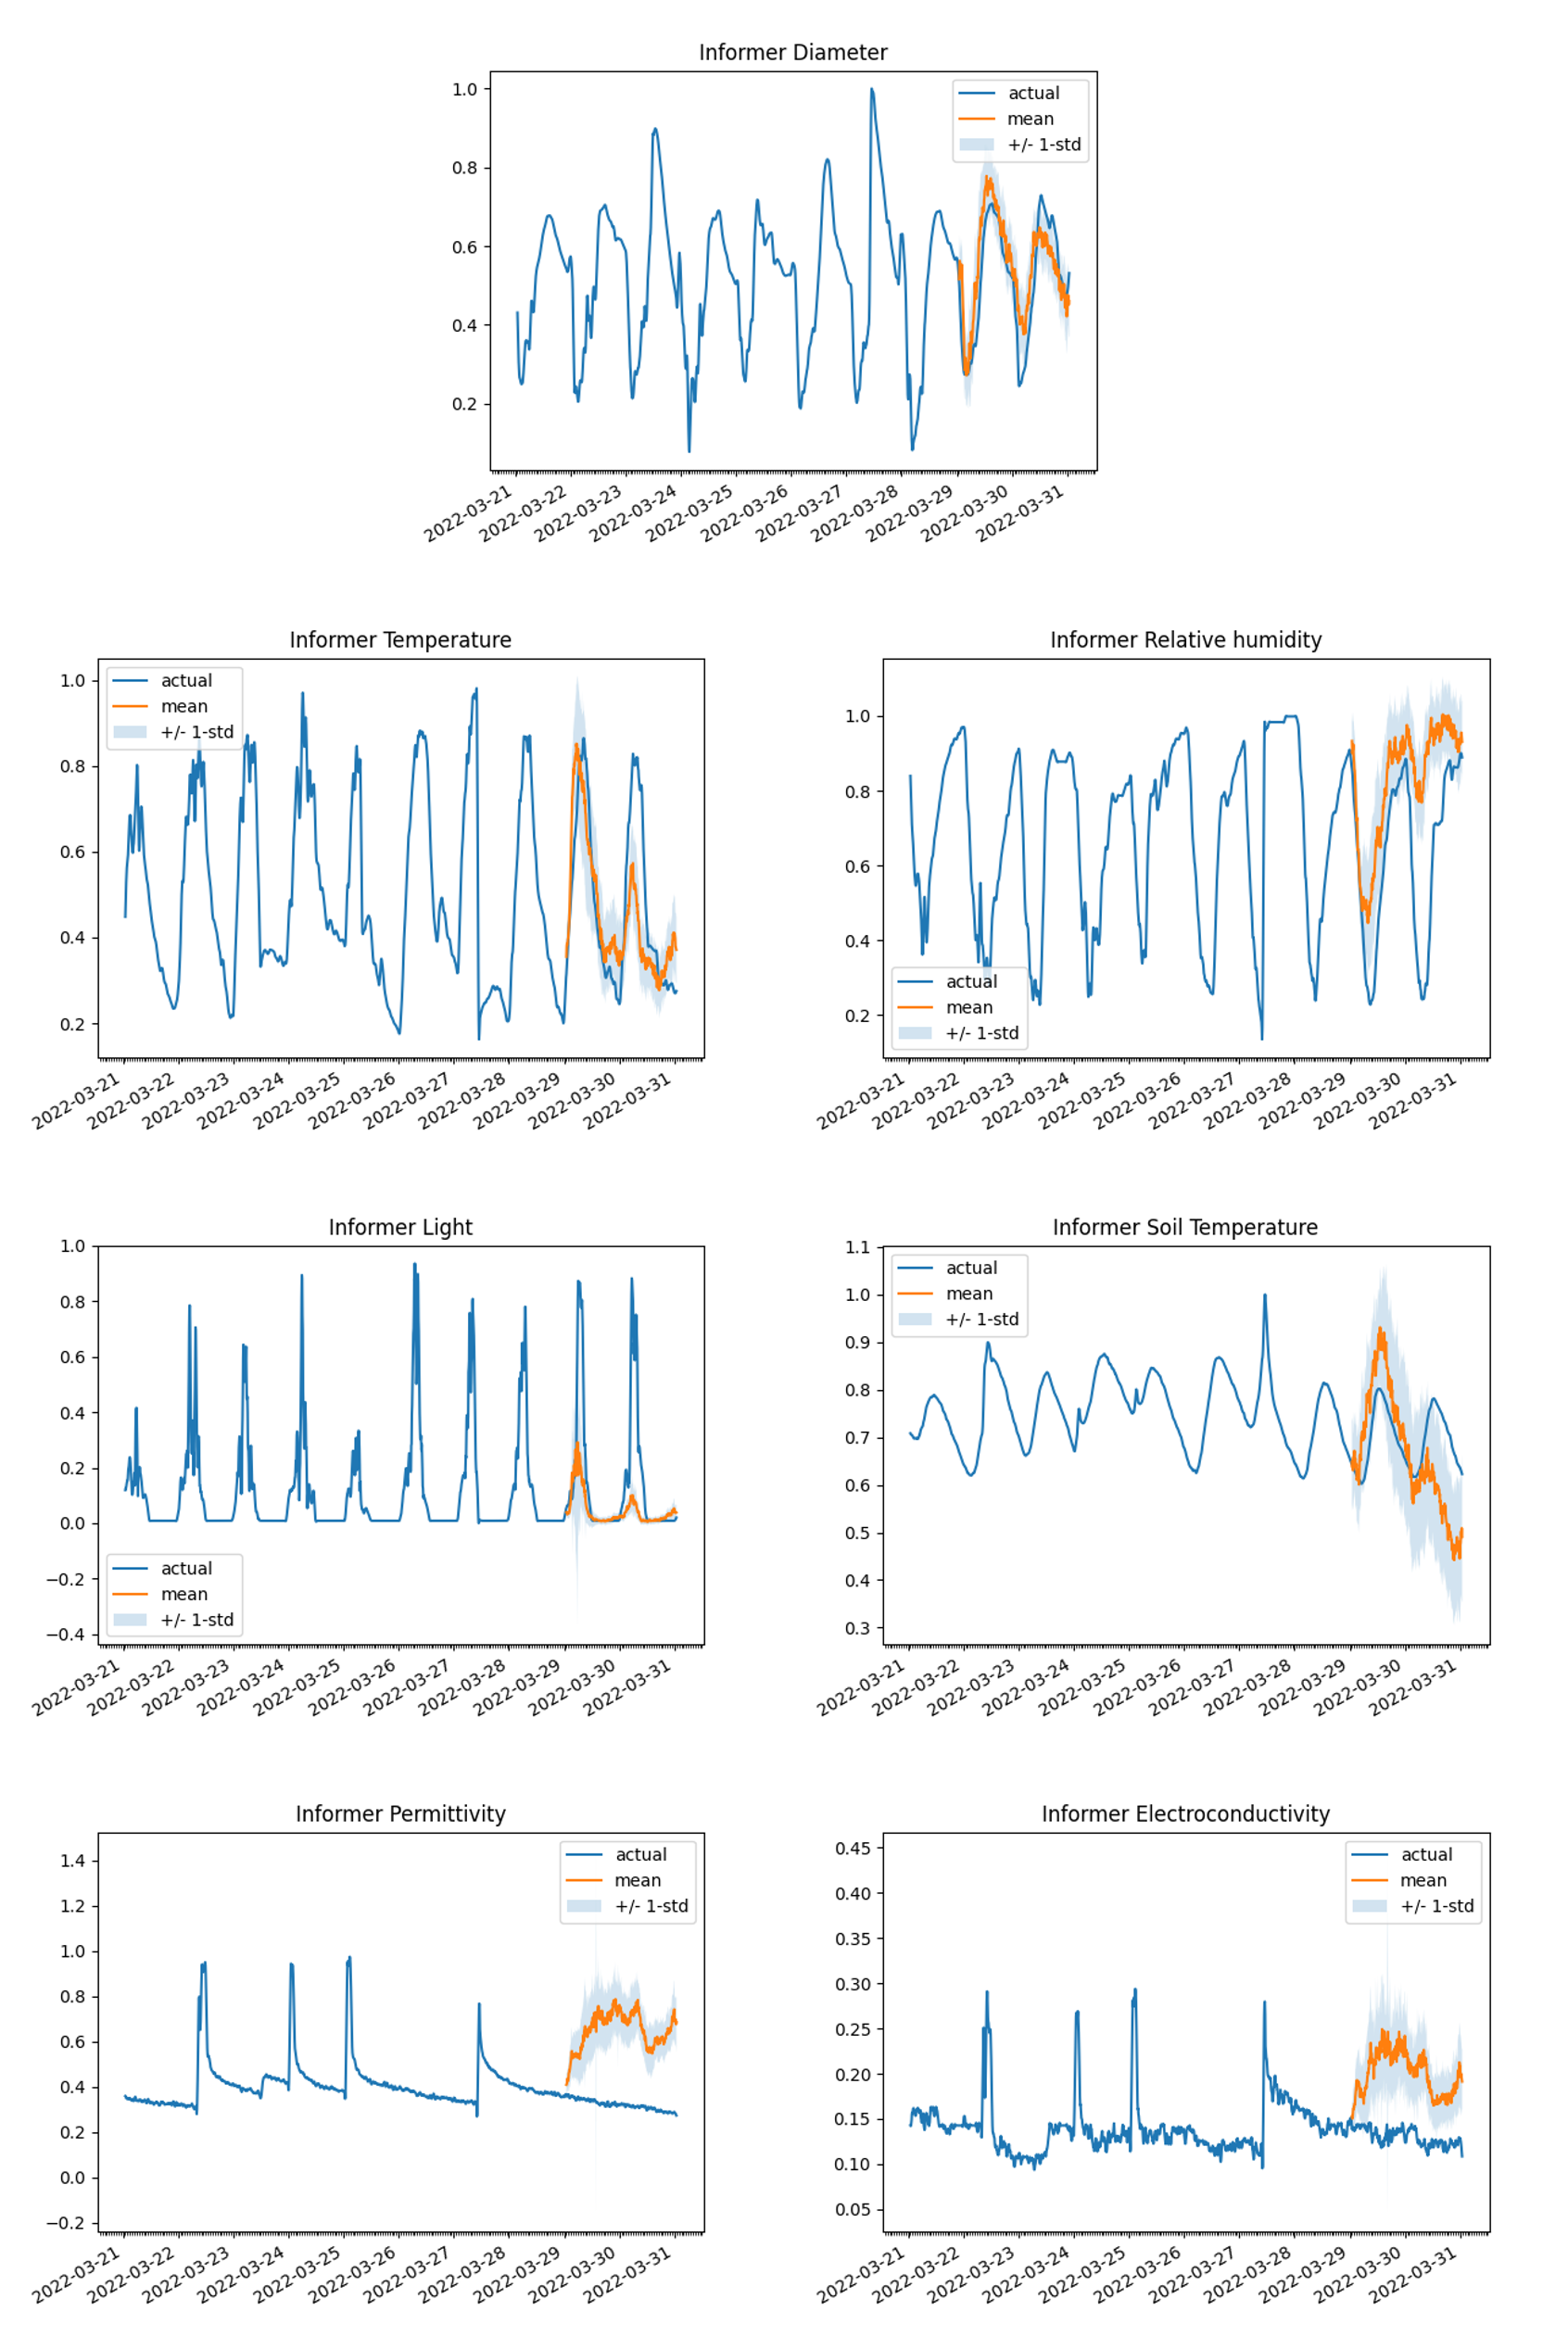
\includegraphics[width=15 cm]{6_ChapterResults/figuras/I20.png}
    \caption{Comparison between the predicted values generated by the I20 model and the actual observed values for the 7 variables over a two-day prediction horizon}
    \label{I20}
\end{figure}

\subsection{Autoformer}
The results for the Autoformer variant with modified Encoder Layers, Decoder Layers, and Dimensionality of the Transformer Layers, as shown in Tables \ref{A4_M} and \ref{A4_R}, reveal a range of performance outcomes when compared to the A11 model, which was used as the baseline for this experimental phase. Similar to the results observed with Transformer and Informer models, the performance across these Autoformer models is quite varied. Among all the models tested, A21 is considered the best due to its particularly strong performance in predicting the diameter. Figure \ref{A21} shows how the predictions from the A21 model align with the actual values, offering insight into the model's performance.

Additionally, as seen in Table \ref{A4_T}, increasing the number of layers leads to higher computational costs, consistent with the patterns observed in both Transformer and Informer models.



\begin{table}[]
    \centering
    \resizebox{\textwidth}{!}{%
    \begin{tabular}{ccccccccc}
    \multicolumn{9}{c}{\textbf{MSE   (Sorted by model)}}                                                                                                                                                                                                                          \\
    Model & Diameter                       & Electroconductivity            & Light                          & Permittivity                   & Relative\_humidity             & Soil\_Temperature              & Temperature                    & Mean                           \\
    A17   & \cellcolor[HTML]{8AC97D}-24.17 & \cellcolor[HTML]{F8696B}-35.47 & \cellcolor[HTML]{FED07F}-11.04 & \cellcolor[HTML]{F4E883}-24.02 & \cellcolor[HTML]{FED580}-16.68 & \cellcolor[HTML]{D5DF81}-21.84 & \cellcolor[HTML]{E3E382}-20.62 & \cellcolor[HTML]{F8E983}-21.98 \\
    A18   & \cellcolor[HTML]{F8696B}-15.94 & \cellcolor[HTML]{F8E983}-37.94 & \cellcolor[HTML]{89C97D}-11.33 & \cellcolor[HTML]{FFE583}-23.71 & \cellcolor[HTML]{F8696B}-12.72 & \cellcolor[HTML]{63BE7B}-24.18 & \cellcolor[HTML]{F8696B}-14.95 & \cellcolor[HTML]{F8696B}-20.11 \\
    A19   & \cellcolor[HTML]{FFE182}-19.12 & \cellcolor[HTML]{AFD37F}-38.86 & \cellcolor[HTML]{ADD37F}-11.29 & \cellcolor[HTML]{FCA477}-22.11 & \cellcolor[HTML]{FB9A75}-14.51 & \cellcolor[HTML]{82C77C}-23.53 & \cellcolor[HTML]{FCAE79}-17.51 & \cellcolor[HTML]{FCA877}-20.99 \\
    A20   & \cellcolor[HTML]{FB9874}-17.17 & \cellcolor[HTML]{FFE784}-37.79 & \cellcolor[HTML]{63BE7B}-11.39 & \cellcolor[HTML]{F8696B}-20.67 & \cellcolor[HTML]{ABD27F}-19.19 & \cellcolor[HTML]{FFDA81}-20.20 & \cellcolor[HTML]{FEC77D}-18.42 & \cellcolor[HTML]{FB9273}-20.69 \\
    A21   & \cellcolor[HTML]{63BE7B}-25.76 & \cellcolor[HTML]{FDB97B}-36.94 & \cellcolor[HTML]{F6E883}-11.19 & \cellcolor[HTML]{CFDD81}-24.59 & \cellcolor[HTML]{FDB67A}-15.54 & \cellcolor[HTML]{FFE383}-20.60 & \cellcolor[HTML]{FEEA83}-19.80 & \cellcolor[HTML]{E8E482}-22.06 \\
    A22   & \cellcolor[HTML]{F8E983}-19.68 & \cellcolor[HTML]{7EC57C}-39.47 & \cellcolor[HTML]{FFDD82}-11.10 & \cellcolor[HTML]{D1DD81}-24.56 & \cellcolor[HTML]{D5DF81}-18.34 & \cellcolor[HTML]{FFE182}-20.51 & \cellcolor[HTML]{FFEB84}-19.77 & \cellcolor[HTML]{FFE984}-21.92 \\
    A23   & \cellcolor[HTML]{FFDC82}-18.99 & \cellcolor[HTML]{FDBF7C}-37.04 & \cellcolor[HTML]{F8696B}-10.50 & \cellcolor[HTML]{FCA878}-22.22 & \cellcolor[HTML]{63BE7B}-20.63 & \cellcolor[HTML]{ECE582}-21.37 & \cellcolor[HTML]{63BE7B}-24.61 & \cellcolor[HTML]{CCDC81}-22.19 \\
    A24   & \cellcolor[HTML]{9BCE7E}-23.45 & \cellcolor[HTML]{63BE7B}-39.80 & \cellcolor[HTML]{FFE984}-11.17 & \cellcolor[HTML]{63BE7B}-26.22 & \cellcolor[HTML]{9FCF7E}-19.41 & \cellcolor[HTML]{F8696B}-15.08 & \cellcolor[HTML]{79C47C}-23.90 & \cellcolor[HTML]{63BE7B}-22.72
    \end{tabular}%
    }
    \caption{Mean Squared Errors (MSE) for different Autoformer models obtained by varying the number of Encoder Layers, Decoder Layers, and Dimensionality of the Transformer Layers, sorted by model}
    \label{A4_M}
    \end{table}



    
\begin{table}[]
    \centering
    \resizebox{\textwidth}{!}{%
    \begin{tabular}{ccccccccc}
    \multicolumn{9}{c}{\textbf{R2 (Sorted by model)}}                                                                                                                                                                                                                     \\
    Model & Diameter                      & Electroconductivity           & Light                         & Permittivity                   & Relative\_humidity            & Soil\_Temperature             & Temperature                  & Mean                          \\
    A17   & \cellcolor[HTML]{78C47D}0.83  & \cellcolor[HTML]{F8696B}-2.50 & \cellcolor[HTML]{FDD17F}-0.38 & \cellcolor[HTML]{F2E884}-7.65  & \cellcolor[HTML]{FEDE81}0.58  & \cellcolor[HTML]{C9DC81}-0.74 & \cellcolor[HTML]{D7E082}0.78 & \cellcolor[HTML]{E2E383}-1.30 \\
    A18   & \cellcolor[HTML]{F8696B}-0.15 & \cellcolor[HTML]{F8E984}-0.98 & \cellcolor[HTML]{89C97E}-0.29 & \cellcolor[HTML]{FEE683}-8.28  & \cellcolor[HTML]{F8696B}-0.06 & \cellcolor[HTML]{63BE7B}-0.02 & \cellcolor[HTML]{F8696B}0.18 & \cellcolor[HTML]{FEEB84}-1.37 \\
    A19   & \cellcolor[HTML]{FEE482}0.45  & \cellcolor[HTML]{A7D27F}-0.60 & \cellcolor[HTML]{ACD380}-0.30 & \cellcolor[HTML]{FBAF78}-12.44 & \cellcolor[HTML]{FBAB77}0.30  & \cellcolor[HTML]{7AC57D}-0.18 & \cellcolor[HTML]{FCBF7B}0.55 & \cellcolor[HTML]{FDC67D}-1.75 \\
    A20   & \cellcolor[HTML]{FBA376}0.14  & \cellcolor[HTML]{FEE783}-1.05 & \cellcolor[HTML]{63BE7B}-0.27 & \cellcolor[HTML]{F8696B}-17.70 & \cellcolor[HTML]{9CCF7F}0.76  & \cellcolor[HTML]{FEE282}-1.54 & \cellcolor[HTML]{FDD37F}0.63 & \cellcolor[HTML]{F8696B}-2.72 \\
    A21   & \cellcolor[HTML]{63BE7B}0.88  & \cellcolor[HTML]{FCC07B}-1.49 & \cellcolor[HTML]{F7E984}-0.33 & \cellcolor[HTML]{C7DB81}-6.60  & \cellcolor[HTML]{FDC67D}0.45  & \cellcolor[HTML]{FEE783}-1.31 & \cellcolor[HTML]{FFEB84}0.73 & \cellcolor[HTML]{94CC7E}-1.10 \\
    A22   & \cellcolor[HTML]{F3E884}0.51  & \cellcolor[HTML]{7AC57D}-0.39 & \cellcolor[HTML]{FEDD81}-0.36 & \cellcolor[HTML]{C9DC81}-6.65  & \cellcolor[HTML]{C7DB81}0.71  & \cellcolor[HTML]{FEE583}-1.37 & \cellcolor[HTML]{FEEA83}0.73 & \cellcolor[HTML]{63BE7B}-0.97 \\
    A23   & \cellcolor[HTML]{FEE082}0.43  & \cellcolor[HTML]{FDC67C}-1.43 & \cellcolor[HTML]{F8696B}-0.56 & \cellcolor[HTML]{FCB379}-12.10 & \cellcolor[HTML]{63BE7B}0.83  & \cellcolor[HTML]{E5E483}-0.94 & \cellcolor[HTML]{63BE7B}0.91 & \cellcolor[HTML]{FCBE7B}-1.84 \\
    A24   & \cellcolor[HTML]{84C87D}0.80  & \cellcolor[HTML]{63BE7B}-0.29 & \cellcolor[HTML]{FEE883}-0.34 & \cellcolor[HTML]{63BE7B}-4.21  & \cellcolor[HTML]{92CC7E}0.77  & \cellcolor[HTML]{F8696B}-7.25 & \cellcolor[HTML]{71C37C}0.90 & \cellcolor[HTML]{FEEA83}-1.37
    \end{tabular}%
    }
    \caption{R-squared (R²) for different Autoformer models obtained by varying the number of Encoder Layers, Decoder Layers, and Dimensionality of the Transformer Layers, sorted by model}
    \label{A4_R}
    \end{table}


    

\begin{table}[]
    \begin{tabular}{ccccc}
    \multicolumn{2}{c}{\textbf{Training   Time (Sorted by model)}} &  & \multicolumn{2}{c}{\textbf{Training Time (Sorted   by training time)}} \\
    Model             & Training time {[}s{]}                      &  & Model                 & Training time {[}s{]}                          \\
    A17               & \cellcolor[HTML]{63BE7B}182.03             &  & A17                   & \cellcolor[HTML]{63BE7B}182.03                 \\
    A18               & \cellcolor[HTML]{E5E382}276.08             &  & A20                   & \cellcolor[HTML]{97CD7E}219.77                 \\
    A19               & \cellcolor[HTML]{FCB279}426.11             &  & A22                   & \cellcolor[HTML]{CDDC81}258.71                 \\
    A20               & \cellcolor[HTML]{97CD7E}219.77             &  & A18                   & \cellcolor[HTML]{E5E382}276.08                 \\
    A21               & \cellcolor[HTML]{FFE483}312.17             &  & A21                   & \cellcolor[HTML]{FFE483}312.17                 \\
    A22               & \cellcolor[HTML]{CDDC81}258.71             &  & A23                   & \cellcolor[HTML]{FECC7E}367.55                 \\
    A23               & \cellcolor[HTML]{FECC7E}367.55             &  & A19                   & \cellcolor[HTML]{FCB279}426.11                 \\
    A24               & \cellcolor[HTML]{F8696B}592.64             &  & A24                   & \cellcolor[HTML]{F8696B}592.64                
    \end{tabular}
    \caption{Training times for different Autoformer models obtained by varying the number of Encoder Layers, Decoder Layers, and Dimensionality of the Transformer Layers, sorted by model and training time values}
    \label{A4_T}
    \end{table}

\begin{figure}[htbp]
    \centering
    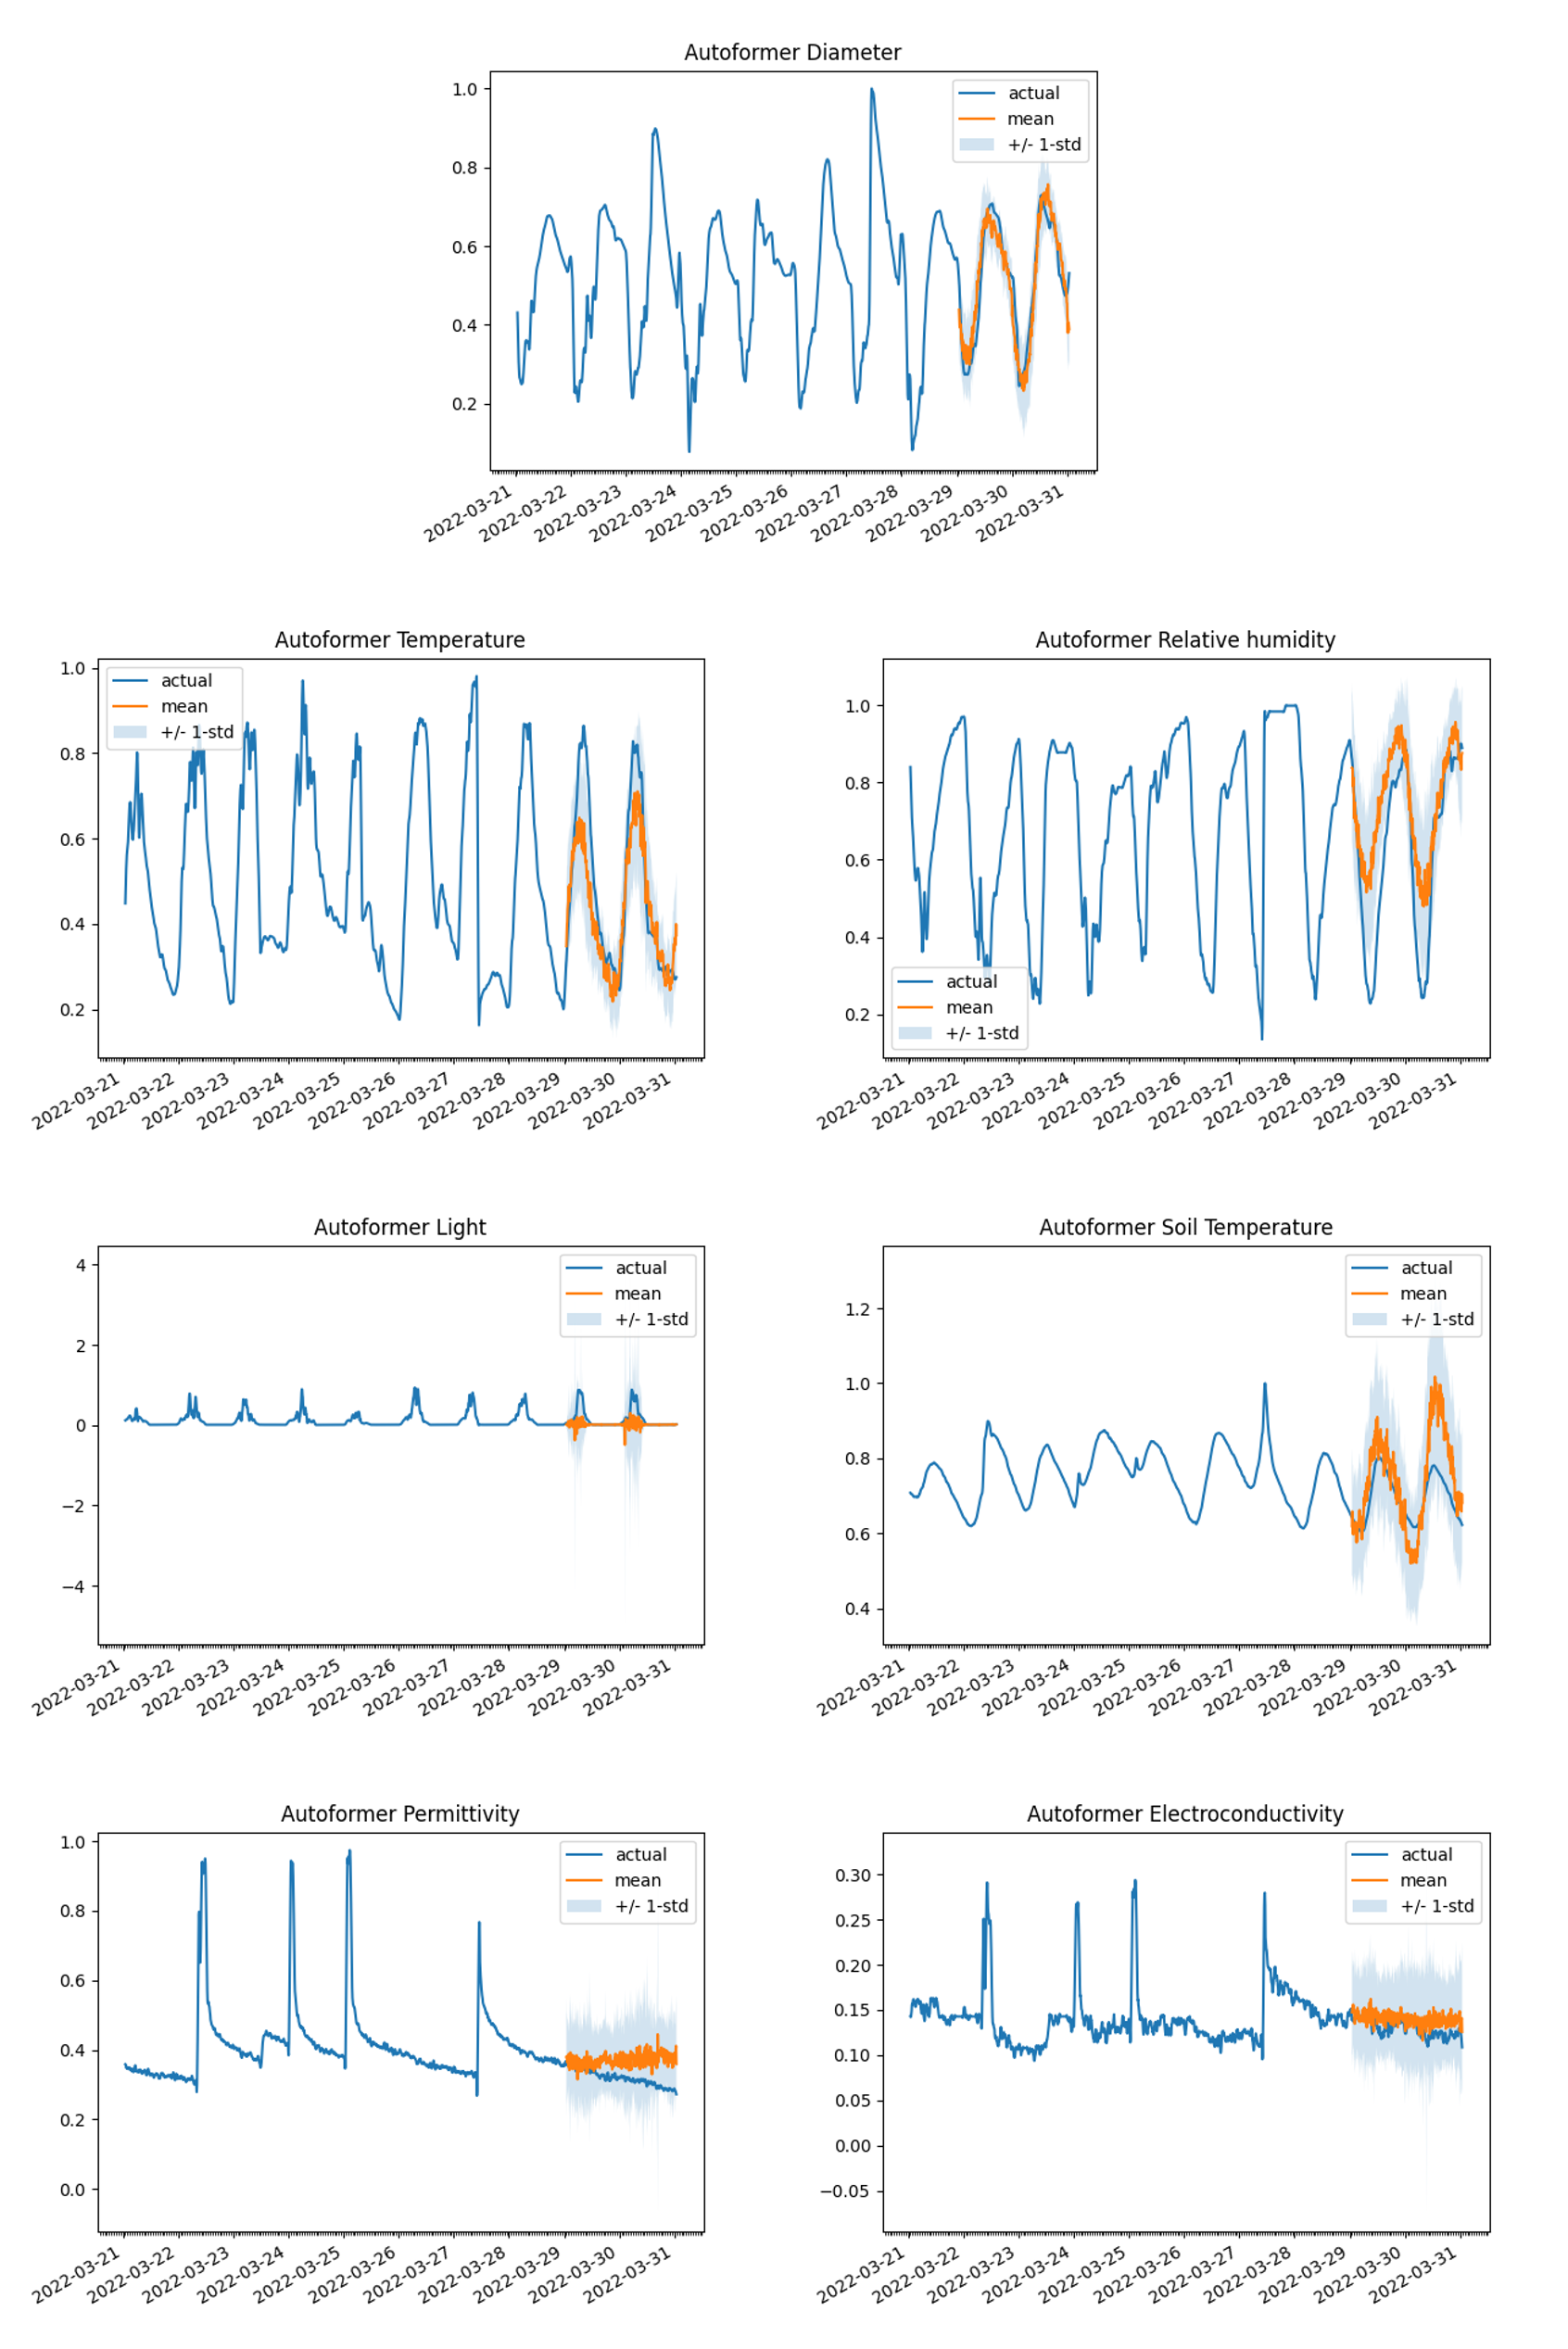
\includegraphics[width=15 cm]{6_ChapterResults/figuras/A21.png}
    \caption{Comparison between the predicted values generated by the A21 model and the actual observed values for the 7 variables over a two-day prediction horizon}
    \label{A21}
\end{figure}

\section{Results Changing the Batch Size and Number of Epochs}
In this section, we present the results of experiments conducted by altering the Batch Size and Number of Epochs across different model variants. These hyperparameters play a crucial role in determining the model's learning process, with Batch Size influencing the number of samples processed before the model’s weights are updated, and Number of Epochs determining the number of times the model iterates over the entire training dataset.

\subsection{Transformer}
The results for the Transformer variant with modified Batch Size and Number of Epochs, as shown in Tables \ref{T5_M} and \ref{T5_R}, exhibit diverse outcomes compared to the T15 model, which was used as the baseline for this experimental phase. Generally, increasing the Batch Size and Number of Epochs leads to improved performance, suggesting that these hyperparameters are crucial for the scalability of Transformer models.

One of the most notable models developed during this phase is the T30 model, which stands out for its strong performance. A detailed comparison of its predictions against the actual values of the seven variables is illustrated in Figure \ref{T30}, demonstrating the model's effectiveness in this experimental setup.

However, as observed in Table \ref{T5_T}, increasing the Batch Size and Number of Epochs also results in higher computational costs and, consequently, longer training times. This trade-off between performance gains and computational efficiency highlights the importance of carefully tuning these hyperparameters to balance accuracy with practical training times.
    

    

\begin{table}[]
    \centering
    \resizebox{\textwidth}{!}{%
    \begin{tabular}{ccccccccc}
    \multicolumn{9}{c}{\textbf{MSE   (Sorted by model)}}                                                                                                                                                                                                                          \\
    Model & Diameter                       & Electroconductivity            & Light                          & Permittivity                   & Relative Humidity              & Soil Temperature               & Temperature                    & Mean                           \\
    T25   & \cellcolor[HTML]{E9E482}-21.84 & \cellcolor[HTML]{F8696B}-19.67 & \cellcolor[HTML]{FDB67A}-13.20 & \cellcolor[HTML]{F8696B}-9.52  & \cellcolor[HTML]{FFEA84}-15.57 & \cellcolor[HTML]{F8696B}-4.95  & \cellcolor[HTML]{FDEA83}-18.15 & \cellcolor[HTML]{F8696B}-14.70 \\
    T26   & \cellcolor[HTML]{F8696B}-17.02 & \cellcolor[HTML]{64BE7B}-35.76 & \cellcolor[HTML]{F8696B}-12.65 & \cellcolor[HTML]{82C67C}-24.94 & \cellcolor[HTML]{F8696B}-9.38  & \cellcolor[HTML]{FFE683}-15.36 & \cellcolor[HTML]{F8696B}-11.96 & \cellcolor[HTML]{FFE383}-18.15 \\
    T27   & \cellcolor[HTML]{FFE082}-21.05 & \cellcolor[HTML]{63BE7B}-35.87 & \cellcolor[HTML]{97CD7E}-14.49 & \cellcolor[HTML]{63BE7B}-25.82 & \cellcolor[HTML]{FBEA83}-15.73 & \cellcolor[HTML]{C3D980}-21.04 & \cellcolor[HTML]{A8D27F}-20.66 & \cellcolor[HTML]{63BE7B}-22.09 \\
    T28   & \cellcolor[HTML]{A8D27F}-23.01 & \cellcolor[HTML]{FFE383}-25.19 & \cellcolor[HTML]{FA8871}-12.87 & \cellcolor[HTML]{7FC67C}-25.03 & \cellcolor[HTML]{FCAF79}-12.71 & \cellcolor[HTML]{F9E983}-16.24 & \cellcolor[HTML]{FCAF79}-15.25 & \cellcolor[HTML]{F5E883}-18.61 \\
    T29   & \cellcolor[HTML]{FCB179}-19.46 & \cellcolor[HTML]{F9E983}-25.98 & \cellcolor[HTML]{D2DE81}-13.97 & \cellcolor[HTML]{FA8972}-12.42 & \cellcolor[HTML]{E3E282}-16.29 & \cellcolor[HTML]{FB9975}-8.94  & \cellcolor[HTML]{FFEB84}-18.08 & \cellcolor[HTML]{FCA777}-16.45 \\
    T30   & \cellcolor[HTML]{63BE7B}-24.28 & \cellcolor[HTML]{FEC87E}-23.97 & \cellcolor[HTML]{63BE7B}-14.94 & \cellcolor[HTML]{FDC57D}-17.90 & \cellcolor[HTML]{63BE7B}-19.24 & \cellcolor[HTML]{63BE7B}-29.52 & \cellcolor[HTML]{63BE7B}-22.70 & \cellcolor[HTML]{6FC17B}-21.79
    \end{tabular}%
    }
    \caption{Mean Squared Errors (MSE) for different Transformer models obtained by varying the Batch Size and Number of Epochs values, sorted by model}
    \label{T5_M}
    \end{table}


    

\begin{table}[]
    \centering
    \resizebox{\textwidth}{!}{%
    \begin{tabular}{ccccccccc}
    \multicolumn{9}{c}{\textbf{R2 (Sorted by model)}}                                                                                                                                                                                                                         \\
    Model & Diameter                     & Electroconductivity             & Light                        & Permittivity                    & Relative\_humidity            & Soil\_Temperature              & Temperature                   & Mean                           \\
    T25   & \cellcolor[HTML]{E3E383}0.70 & \cellcolor[HTML]{F8696B}-131.83 & \cellcolor[HTML]{FCBA7A}0.16 & \cellcolor[HTML]{F8696B}-242.90 & \cellcolor[HTML]{FEEA83}0.45  & \cellcolor[HTML]{F8696B}-83.96 & \cellcolor[HTML]{FDEB84}0.61  & \cellcolor[HTML]{F8696B}-65.25 \\
    T26   & \cellcolor[HTML]{F8696B}0.11 & \cellcolor[HTML]{64BF7C}-2.27   & \cellcolor[HTML]{F8696B}0.05 & \cellcolor[HTML]{70C27C}-6.00   & \cellcolor[HTML]{F8696B}-1.28 & \cellcolor[HTML]{FEE983}-6.74  & \cellcolor[HTML]{F8696B}-0.62 & \cellcolor[HTML]{82C77D}-2.39  \\
    T27   & \cellcolor[HTML]{FEE482}0.65 & \cellcolor[HTML]{63BE7B}-2.19   & \cellcolor[HTML]{92CC7E}0.38 & \cellcolor[HTML]{63BE7B}-4.72   & \cellcolor[HTML]{FBEA84}0.47  & \cellcolor[HTML]{8DCA7E}-1.09  & \cellcolor[HTML]{95CD7E}0.78  & \cellcolor[HTML]{63BE7B}-0.82  \\
    T28   & \cellcolor[HTML]{9DCF7F}0.77 & \cellcolor[HTML]{FEE683}-36.29  & \cellcolor[HTML]{F98A71}0.10 & \cellcolor[HTML]{6FC27C}-5.87   & \cellcolor[HTML]{FCC47C}-0.06 & \cellcolor[HTML]{EFE784}-5.32  & \cellcolor[HTML]{FCC47C}0.24  & \cellcolor[HTML]{D3DF82}-6.63  \\
    T29   & \cellcolor[HTML]{FCC07B}0.49 & \cellcolor[HTML]{F0E784}-30.12  & \cellcolor[HTML]{CDDD82}0.30 & \cellcolor[HTML]{FBAE78}-123.95 & \cellcolor[HTML]{D9E082}0.54  & \cellcolor[HTML]{FCBE7B}-32.95 & \cellcolor[HTML]{FEEA83}0.60  & \cellcolor[HTML]{FCC27C}-26.44 \\
    T30   & \cellcolor[HTML]{63BE7B}0.83 & \cellcolor[HTML]{FDD780}-48.35  & \cellcolor[HTML]{63BE7B}0.44 & \cellcolor[HTML]{FEE282}-34.42  & \cellcolor[HTML]{63BE7B}0.77  & \cellcolor[HTML]{63BE7B}0.70   & \cellcolor[HTML]{63BE7B}0.86  & \cellcolor[HTML]{FEE582}-11.31
    \end{tabular}%
    }
    \caption{R-squared (R²) for different Transformer models obtained by varying the Batch Size and Number of Epochs values, sorted by model}
    \label{T5_R}
    \end{table}



    
\begin{table}[]
    \begin{tabular}{ccccc}
    \multicolumn{2}{c}{\textbf{Training   Time (Sorted by model)}} &  & \multicolumn{2}{c}{\textbf{Training Time (Sorted   by training time)}} \\
    Model             & Training time {[}s{]}                      &  & Model                 & Training time {[}s{]}                          \\
    T25               & \cellcolor[HTML]{63BE7B}130.65             &  & T25                   & \cellcolor[HTML]{63BE7B}130.65                 \\
    T26               & \cellcolor[HTML]{E3E382}387.01             &  & T27                   & \cellcolor[HTML]{9DCF7E}248.18                 \\
    T27               & \cellcolor[HTML]{9DCF7E}248.18             &  & T26                   & \cellcolor[HTML]{E3E382}387.01                 \\
    T28               & \cellcolor[HTML]{FDC67D}756.21             &  & T29                   & \cellcolor[HTML]{FFE583}495.93                 \\
    T29               & \cellcolor[HTML]{FFE583}495.93             &  & T28                   & \cellcolor[HTML]{FDC67D}756.21                 \\
    T30               & \cellcolor[HTML]{F8696B}1542.75            &  & T30                   & \cellcolor[HTML]{F8696B}1542.75               
    \end{tabular}
    \caption{Training times for different Transformer models obtained by varying the Batch Size and Number of Epochs values, sorted by model and training time values}
    \label{T5_T}
    \end{table}

\begin{figure}[htbp]
    \centering
    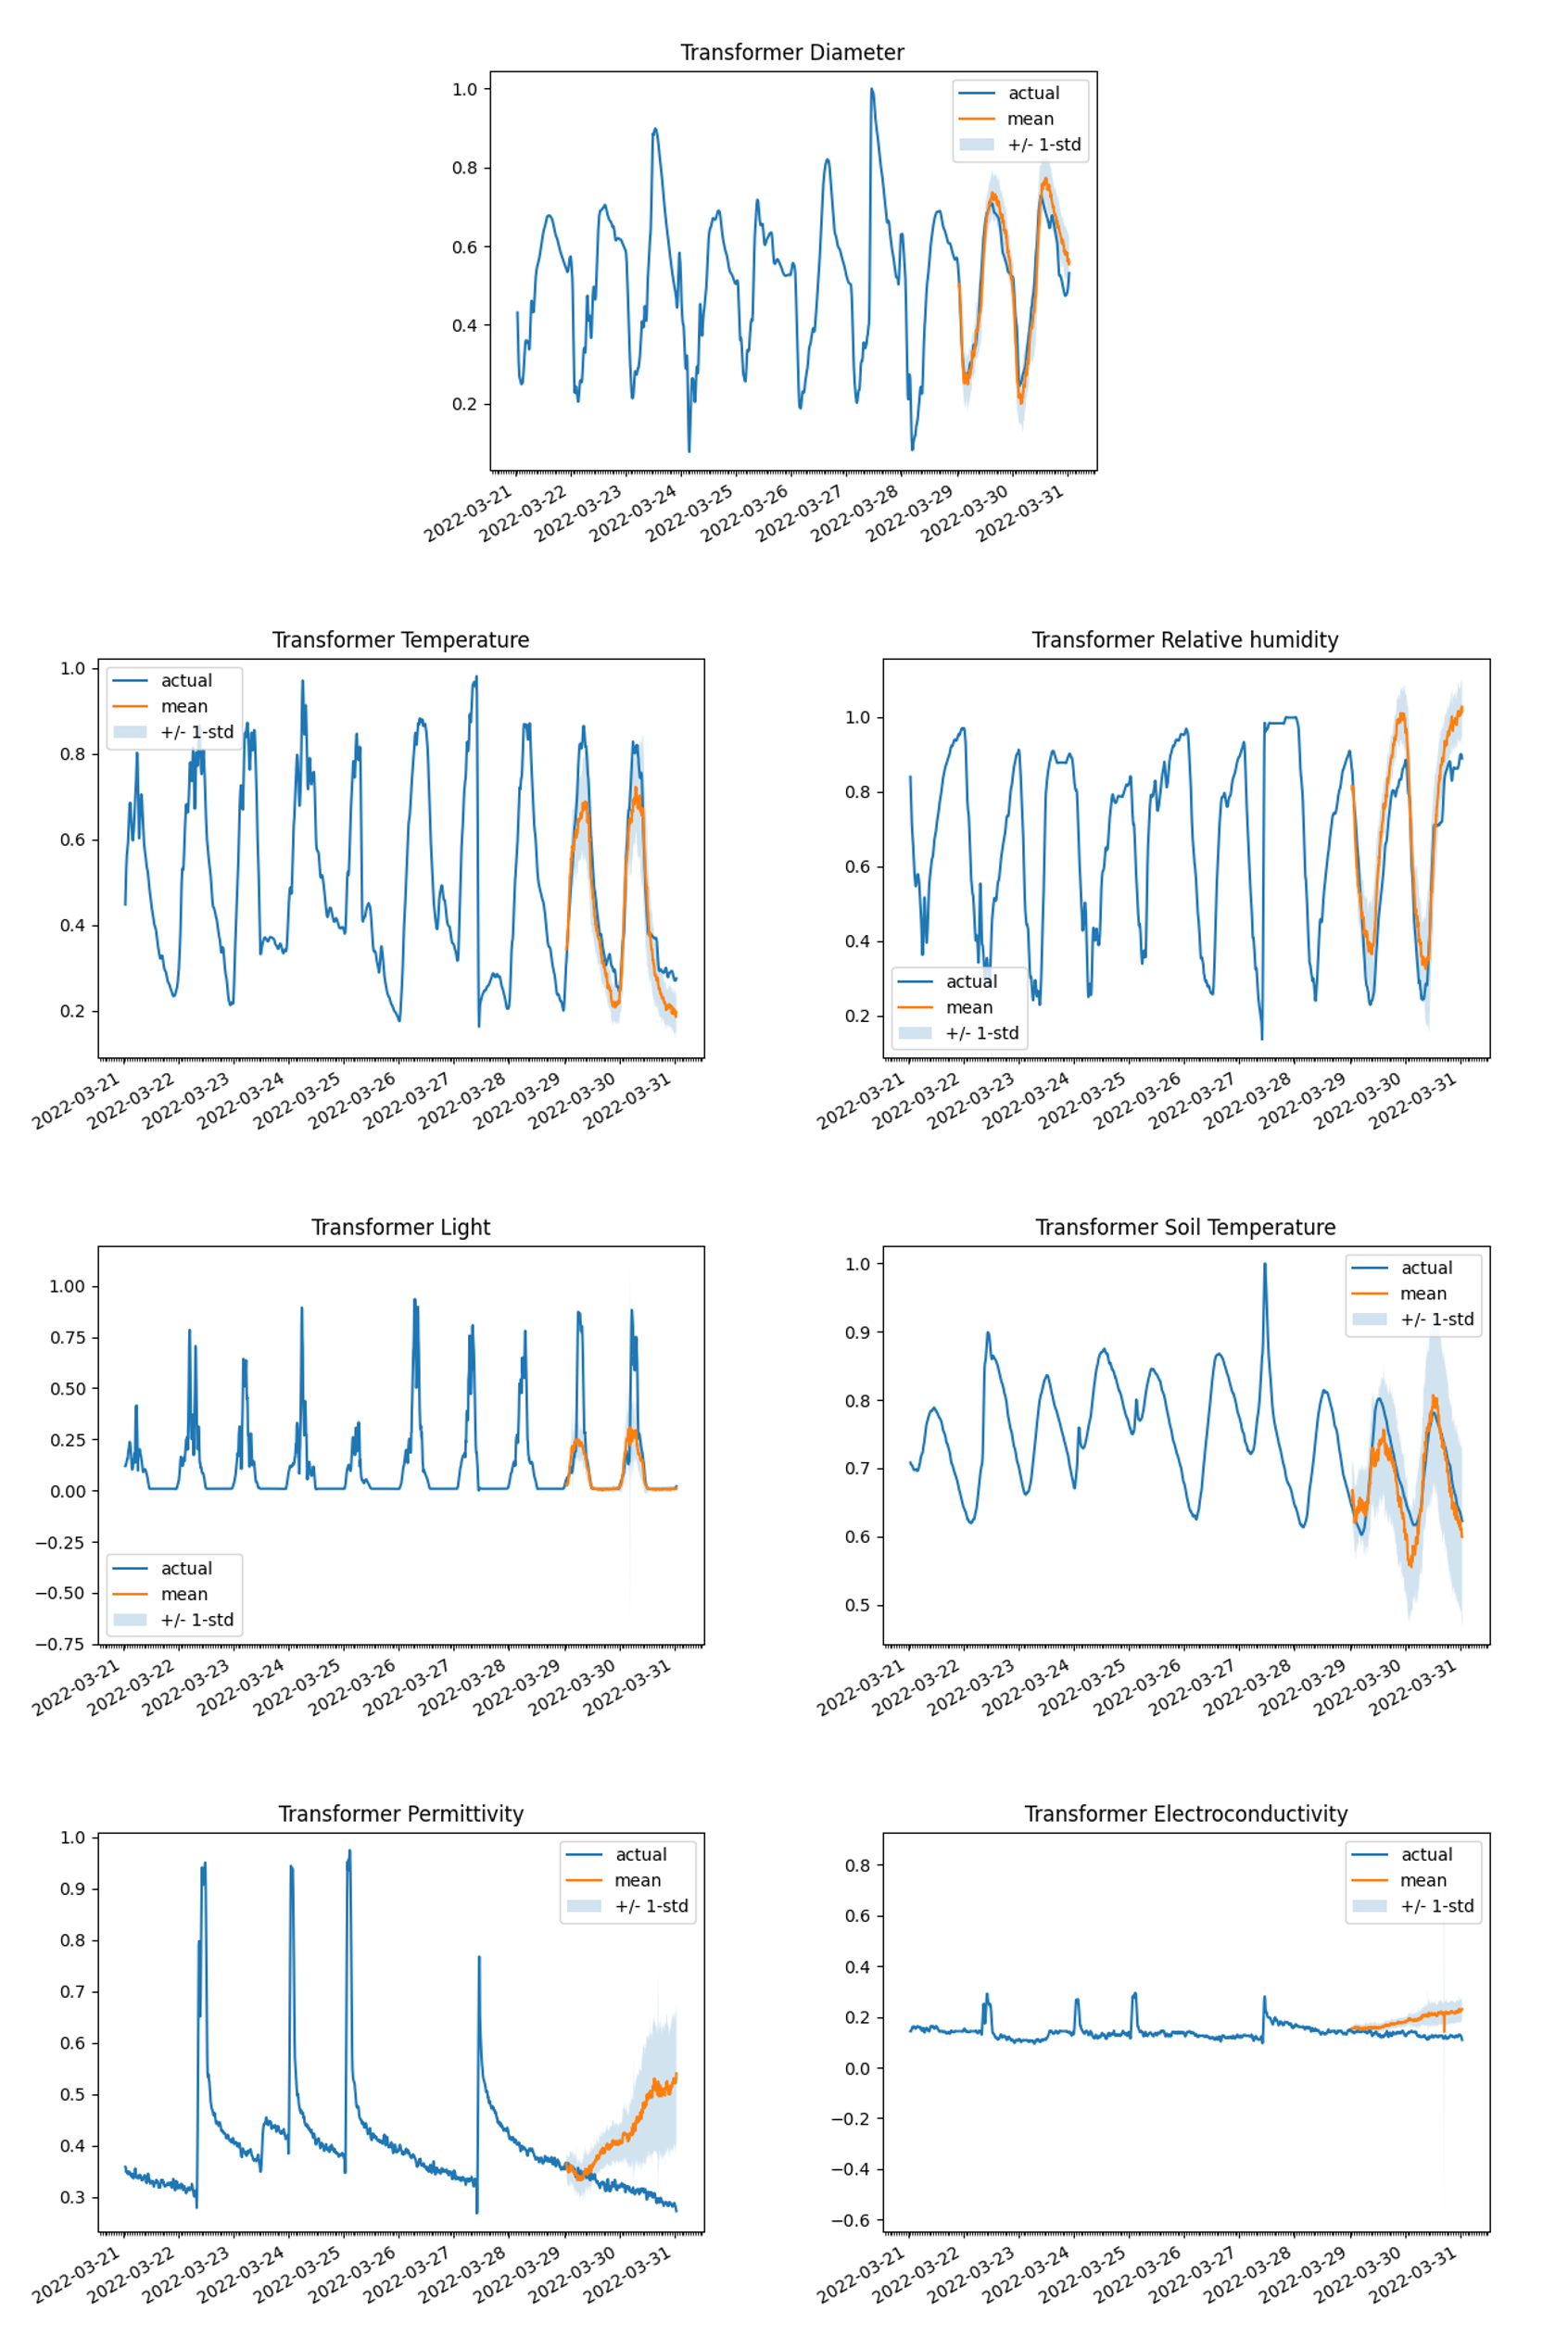
\includegraphics[width=15 cm]{6_ChapterResults/figuras/T30.png}
    \caption{Comparison between the predicted values generated by the T30 model and the actual observed values for the 7 variables over a two-day prediction horizon}
    \label{T30}
\end{figure}

\subsection{Informer}
The results for the Informer variant with modified Batch Size and Number of Epochs, as shown in Tables \ref{I5_M} and \ref{I5_R}, display varied outcomes compared to the I20 model, which served as the baseline for this experimental phase. Generally, increasing the Batch Size and Number of Epochs leads to improved performance, similar to what was observed with the Transformer models. This indicates that these hyperparameters are also important for optimizing the Informer's predictive capabilities.

Among the models evaluated in this phase, the I30 model emerged as a top performer, showing remarkable accuracy in predictions. Figure \ref{I30} provides a visual comparison between the predicted and actual values of the seven variables, underscoring the model's success in this phase of the experiment.

However, as seen in Table \ref{I5_T}, increasing the Batch Size and Number of Epochs results in higher computational costs and longer training times. Despite this, the Informer remains more efficient compared to the Transformer, maintaining better computational efficiency even with these adjustments.
    

    
\begin{table}[]
    \centering
    \resizebox{\textwidth}{!}{%
    \begin{tabular}{ccccccccc}
    \multicolumn{9}{c}{\textbf{MSE   (Sorted by model)}}                                                                                                                                                                                                                          \\
    Model & Diameter                       & Electroconductivity            & Light                          & Permittivity                   & Relative\_humidity             & Soil\_Temperature              & Temperature                    & Mean                           \\
    I25   & \cellcolor[HTML]{F8696B}-16.77 & \cellcolor[HTML]{FCAA78}-29.75 & \cellcolor[HTML]{FDBD7B}-12.62 & \cellcolor[HTML]{FB9975}-15.51 & \cellcolor[HTML]{F8696B}-11.20 & \cellcolor[HTML]{FB9073}-10.05 & \cellcolor[HTML]{F8696B}-9.60  & \cellcolor[HTML]{F8696B}-15.07 \\
    I26   & \cellcolor[HTML]{C2D980}-22.58 & \cellcolor[HTML]{FFE383}-35.67 & \cellcolor[HTML]{A3D07E}-13.74 & \cellcolor[HTML]{63BE7B}-29.67 & \cellcolor[HTML]{88C87D}-16.02 & \cellcolor[HTML]{98CD7E}-26.51 & \cellcolor[HTML]{AAD27F}-18.55 & \cellcolor[HTML]{6DC17B}-23.25 \\
    I27   & \cellcolor[HTML]{FEC97E}-19.74 & \cellcolor[HTML]{DBE081}-37.34 & \cellcolor[HTML]{F8696B}-12.19 & \cellcolor[HTML]{C5DA80}-26.03 & \cellcolor[HTML]{E2E282}-13.88 & \cellcolor[HTML]{F8696B}-6.48  & \cellcolor[HTML]{FB9474}-11.65 & \cellcolor[HTML]{FED380}-18.19 \\
    I28   & \cellcolor[HTML]{63BE7B}-25.39 & \cellcolor[HTML]{F8696B}-23.12 & \cellcolor[HTML]{E5E382}-13.11 & \cellcolor[HTML]{F8696B}-10.63 & \cellcolor[HTML]{FDBE7C}-12.50 & \cellcolor[HTML]{A3D07E}-25.60 & \cellcolor[HTML]{A4D07E}-18.75 & \cellcolor[HTML]{FFDC82}-18.44 \\
    I29   & \cellcolor[HTML]{FDC27D}-19.52 & \cellcolor[HTML]{63BE7B}-40.22 & \cellcolor[HTML]{FCB079}-12.55 & \cellcolor[HTML]{C2D980}-26.13 & \cellcolor[HTML]{FDC07C}-12.53 & \cellcolor[HTML]{FB9F76}-11.41 & \cellcolor[HTML]{FCB37A}-13.11 & \cellcolor[HTML]{EFE683}-19.35 \\
    I30   & \cellcolor[HTML]{DBE081}-21.86 & \cellcolor[HTML]{AAD27F}-38.52 & \cellcolor[HTML]{63BE7B}-14.36 & \cellcolor[HTML]{FED780}-21.75 & \cellcolor[HTML]{63BE7B}-16.90 & \cellcolor[HTML]{63BE7B}-30.65 & \cellcolor[HTML]{63BE7B}-20.88 & \cellcolor[HTML]{63BE7B}-23.56
    \end{tabular}%
    }
    \caption{Mean Squared Errors (MSE) for different Informer models obtained by varying the Batch Size and Number of Epochs values, sorted by model}
    \label{I5_M}
    \end{table}


    
\begin{table}[]
    \centering
    \resizebox{\textwidth}{!}{%
    \begin{tabular}{ccccccccc}
    \multicolumn{9}{c}{\textbf{R2 (Sorted by model)}}                                                                                                                                                                                                                         \\
    Model & Diameter                     & Electroconductivity            & Light                         & Permittivity                    & Relative\_humidity            & Soil\_Temperature              & Temperature                   & Mean                           \\
    I25   & \cellcolor[HTML]{F8696B}0.05 & \cellcolor[HTML]{FDD37F}-12.06 & \cellcolor[HTML]{FCBF7B}0.05  & \cellcolor[HTML]{FCC57C}-60.38  & \cellcolor[HTML]{F8696B}-0.50 & \cellcolor[HTML]{FCC07B}-25.26 & \cellcolor[HTML]{F8696B}-1.80 & \cellcolor[HTML]{FDC67D}-14.27 \\
    I26   & \cellcolor[HTML]{ACD380}0.75 & \cellcolor[HTML]{FEE983}-2.34  & \cellcolor[HTML]{9DCF7F}0.26  & \cellcolor[HTML]{63BE7B}-1.36   & \cellcolor[HTML]{7DC67D}0.51  & \cellcolor[HTML]{69C07C}0.41   & \cellcolor[HTML]{8ACA7E}0.64  & \cellcolor[HTML]{63BE7B}-0.16  \\
    I27   & \cellcolor[HTML]{FDD57F}0.52 & \cellcolor[HTML]{CCDD82}-1.27  & \cellcolor[HTML]{F8696B}-0.06 & \cellcolor[HTML]{A2D17F}-4.45   & \cellcolor[HTML]{D6E082}0.19  & \cellcolor[HTML]{F8696B}-58.73 & \cellcolor[HTML]{FBAD78}-0.75 & \cellcolor[HTML]{FEDD81}-9.22  \\
    I28   & \cellcolor[HTML]{63BE7B}0.87 & \cellcolor[HTML]{F8696B}-59.13 & \cellcolor[HTML]{E2E383}0.15  & \cellcolor[HTML]{F8696B}-188.09 & \cellcolor[HTML]{FCC57C}-0.11 & \cellcolor[HTML]{6CC17C}0.27   & \cellcolor[HTML]{86C97E}0.66  & \cellcolor[HTML]{F8696B}-35.05 \\
    I29   & \cellcolor[HTML]{FDCF7E}0.50 & \cellcolor[HTML]{63BE7B}-0.17  & \cellcolor[HTML]{FBB279}0.03  & \cellcolor[HTML]{A0D07F}-4.33   & \cellcolor[HTML]{FDC77D}-0.11 & \cellcolor[HTML]{FDD27F}-18.22 & \cellcolor[HTML]{FDCD7E}-0.25 & \cellcolor[HTML]{B2D580}-3.22  \\
    I30   & \cellcolor[HTML]{C7DB81}0.71 & \cellcolor[HTML]{99CE7F}-0.73  & \cellcolor[HTML]{63BE7B}0.36  & \cellcolor[HTML]{FEE783}-13.59  & \cellcolor[HTML]{63BE7B}0.60  & \cellcolor[HTML]{63BE7B}0.77   & \cellcolor[HTML]{63BE7B}0.79  & \cellcolor[HTML]{88C97E}-1.59 
    \end{tabular}%
    }
    \caption{R-squared (R²) for different Informer models obtained by varying the Batch Size and Number of Epochs values, sorted by model}
    \label{I5_R}
    \end{table}



\begin{table}[]
    \begin{tabular}{ccccc}
    \multicolumn{2}{c}{\textbf{Training   Time (Sorted by model)}} &  & \multicolumn{2}{c}{\textbf{Training Time (Sorted   by training time)}} \\
    Model             & Training time {[}s{]}                      &  & Model                 & Training time {[}s{]}                          \\
    I25               & \cellcolor[HTML]{63BE7B}59.53              &  & I25                   & \cellcolor[HTML]{63BE7B}59.53                  \\
    I26               & \cellcolor[HTML]{FFE784}163.53             &  & I27                   & \cellcolor[HTML]{90CB7D}86.82                  \\
    I27               & \cellcolor[HTML]{90CB7D}86.82              &  & I29                   & \cellcolor[HTML]{EDE582}142.6                  \\
    I28               & \cellcolor[HTML]{FDBC7B}255.43             &  & I26                   & \cellcolor[HTML]{FFE784}163.53                 \\
    I29               & \cellcolor[HTML]{EDE582}142.6              &  & I28                   & \cellcolor[HTML]{FDBC7B}255.43                 \\
    I30               & \cellcolor[HTML]{F8696B}432.91             &  & I30                   & \cellcolor[HTML]{F8696B}432.91                
    \end{tabular}
    \caption{Training times for different Informer models obtained by varying the Batch Size and Number of Epochs values, sorted by model and training time values}
    \label{I5_T}
    \end{table}

\begin{figure}[htbp]
    \centering
    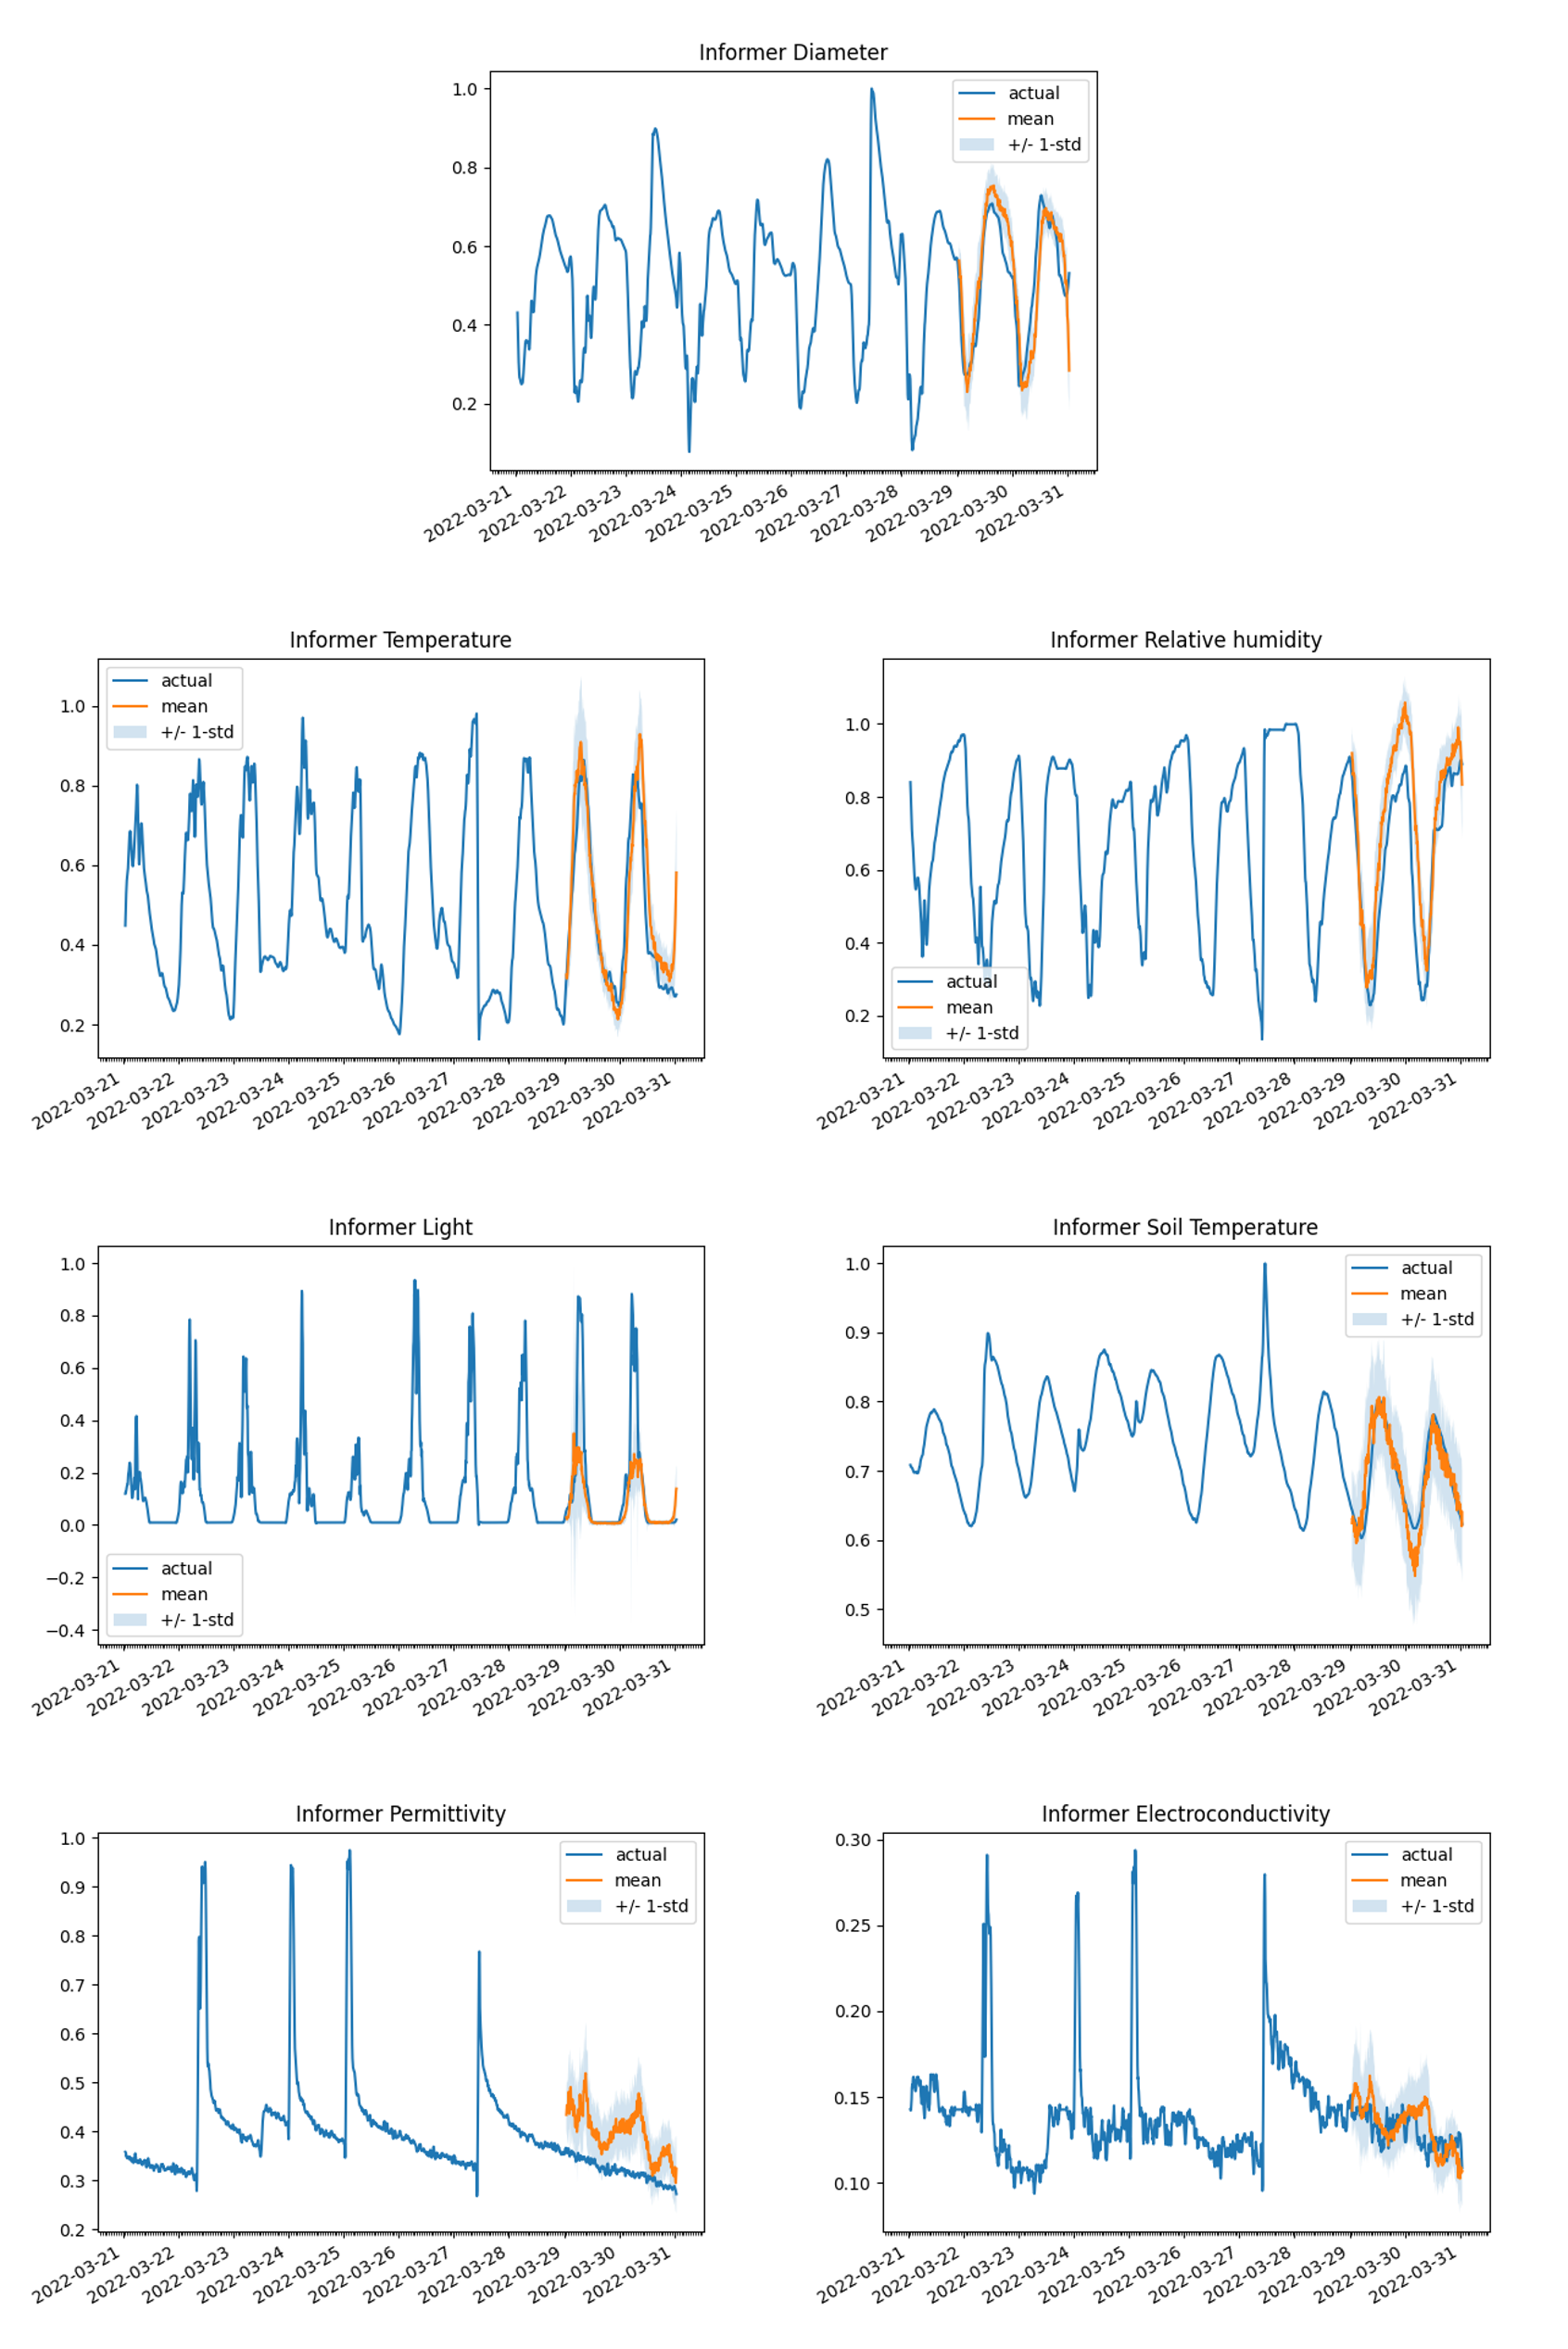
\includegraphics[width=15 cm]{6_ChapterResults/figuras/I30.png}
    \caption{Comparison between the predicted values generated by the I30 model and the actual observed values for the 7 variables over a two-day prediction horizon}
    \label{I30}
\end{figure}

\subsection{Autoformer}
The results for the Autoformer variant with modified Batch Size and Number of Epochs, as shown in Tables \ref{A5_M} and \ref{A5_R}, exhibit varied outcomes compared to the A21 model, which served as the baseline for this experimental phase. In this case, the modifications did not lead to significant improvements over the previous models.

The A29 model, recognized as one of the best outcomes in this phase, has shown significant predictive capability. This is evident in Figure \ref{A29}, where a comparison between the model's predictions and the actual values for the seven variables is presented, highlighting its superior performance.

However, as observed in Table \ref{A5_T}, similar to the results with Transformers and Informers, increasing the Batch Size and Number of Epochs results in higher computational costs and, consequently, longer training times. This highlights the trade-off between potentially better performance and increased computational demands when adjusting these hyperparameters.
    


\begin{table}[]
    \centering
    \resizebox{\textwidth}{!}{%
    \begin{tabular}{ccccccccc}
    \multicolumn{9}{c}{\textbf{MSE   (Sorted by model)}}                                                                                                                                                                                                                          \\
    Model & Diameter                       & Electroconductivity            & Light                          & Permittivity                   & Relative\_humidity             & Soil\_Temperature              & Temperature                    & Mean                           \\
    A25   & \cellcolor[HTML]{FB9073}-19.10 & \cellcolor[HTML]{63BE7B}-39.74 & \cellcolor[HTML]{F8696B}-11.07 & \cellcolor[HTML]{FCA878}-20.41 & \cellcolor[HTML]{FFE683}-16.46 & \cellcolor[HTML]{FCA276}-16.73 & \cellcolor[HTML]{FCB37A}-17.69 & \cellcolor[HTML]{FCB279}-20.17 \\
    A26   & \cellcolor[HTML]{F7E883}-21.55 & \cellcolor[HTML]{FBE983}-38.41 & \cellcolor[HTML]{FDC67D}-11.16 & \cellcolor[HTML]{FEEA83}-21.47 & \cellcolor[HTML]{E1E282}-17.06 & \cellcolor[HTML]{63BE7B}-21.72 & \cellcolor[HTML]{63BE7B}-23.03 & \cellcolor[HTML]{A2D07E}-22.06 \\
    A27   & \cellcolor[HTML]{FFE884}-21.39 & \cellcolor[HTML]{FCAA78}-36.98 & \cellcolor[HTML]{63BE7B}-11.34 & \cellcolor[HTML]{63BE7B}-28.37 & \cellcolor[HTML]{FED17F}-15.40 & \cellcolor[HTML]{F8696B}-15.05 & \cellcolor[HTML]{91CB7D}-22.38 & \cellcolor[HTML]{FFEA84}-21.56 \\
    A28   & \cellcolor[HTML]{F8696B}-18.12 & \cellcolor[HTML]{F8696B}-35.60 & \cellcolor[HTML]{FFDC81}-11.18 & \cellcolor[HTML]{F8696B}-19.47 & \cellcolor[HTML]{F8696B}-9.98  & \cellcolor[HTML]{91CB7D}-20.90 & \cellcolor[HTML]{F8696B}-13.50 & \cellcolor[HTML]{F8696B}-18.39 \\
    A29   & \cellcolor[HTML]{63BE7B}-23.10 & \cellcolor[HTML]{8FCA7D}-39.35 & \cellcolor[HTML]{DEE182}-11.23 & \cellcolor[HTML]{95CC7D}-26.12 & \cellcolor[HTML]{D6DF81}-17.17 & \cellcolor[HTML]{FDB57A}-17.33 & \cellcolor[HTML]{99CD7E}-22.28 & \cellcolor[HTML]{63BE7B}-22.37 \\
    A30   & \cellcolor[HTML]{C4DA80}-22.07 & \cellcolor[HTML]{FFEA84}-38.34 & \cellcolor[HTML]{EDE582}-11.21 & \cellcolor[HTML]{FFE984}-21.39 & \cellcolor[HTML]{63BE7B}-18.35 & \cellcolor[HTML]{A2D07E}-20.60 & \cellcolor[HTML]{FED380}-19.50 & \cellcolor[HTML]{F7E883}-21.64
    \end{tabular}%
    }
    \caption{Mean Squared Errors (MSE) for different Autoformer models obtained by varying the Batch Size and Number of Epochs values, sorted by model}
    \label{A5_M}
    \end{table}



    
\begin{table}[]
    \centering
    \resizebox{\textwidth}{!}{%
    \begin{tabular}{ccccccccc}
    \multicolumn{9}{c}{\textbf{R2 (Sorted by model)}}                                                                                                                                                                                                                     \\
    Model & Diameter                     & Electroconductivity           & Light                         & Permittivity                   & Relative\_humidity            & Soil\_Temperature             & Temperature                   & Mean                          \\
    A25   & \cellcolor[HTML]{FA9A74}0.45 & \cellcolor[HTML]{63BE7B}-0.31 & \cellcolor[HTML]{F8696B}-0.37 & \cellcolor[HTML]{FBAE78}-18.85 & \cellcolor[HTML]{FEE883}0.55  & \cellcolor[HTML]{FBB379}-4.64 & \cellcolor[HTML]{FDCC7E}0.57  & \cellcolor[HTML]{FA9F75}-3.23 \\
    A26   & \cellcolor[HTML]{F6E984}0.68 & \cellcolor[HTML]{FBEA84}-0.78 & \cellcolor[HTML]{FCC47C}-0.34 & \cellcolor[HTML]{FEEB84}-14.57 & \cellcolor[HTML]{DCE182}0.61  & \cellcolor[HTML]{63BE7B}-0.79 & \cellcolor[HTML]{63BE7B}0.87  & \cellcolor[HTML]{F7E984}-2.04 \\
    A27   & \cellcolor[HTML]{FEE883}0.67 & \cellcolor[HTML]{FCB479}-1.47 & \cellcolor[HTML]{63BE7B}-0.28 & \cellcolor[HTML]{63BE7B}-2.18  & \cellcolor[HTML]{FEDE81}0.43  & \cellcolor[HTML]{F8696B}-7.32 & \cellcolor[HTML]{86C87D}0.85  & \cellcolor[HTML]{95CD7E}-1.33 \\
    A28   & \cellcolor[HTML]{F8696B}0.30 & \cellcolor[HTML]{F8696B}-2.40 & \cellcolor[HTML]{FEDB80}-0.33 & \cellcolor[HTML]{F8696B}-23.65 & \cellcolor[HTML]{F8696B}-0.99 & \cellcolor[HTML]{84C87D}-1.16 & \cellcolor[HTML]{F8696B}-0.14 & \cellcolor[HTML]{F8696B}-4.05 \\
    A29   & \cellcolor[HTML]{63BE7B}0.78 & \cellcolor[HTML]{8BCA7E}-0.43 & \cellcolor[HTML]{DEE283}-0.32 & \cellcolor[HTML]{7EC67D}-4.33  & \cellcolor[HTML]{D0DE82}0.62  & \cellcolor[HTML]{FDC77D}-3.91 & \cellcolor[HTML]{8CCA7E}0.85  & \cellcolor[HTML]{63BE7B}-0.96 \\
    A30   & \cellcolor[HTML]{BFD981}0.72 & \cellcolor[HTML]{FEE983}-0.81 & \cellcolor[HTML]{EDE683}-0.32 & \cellcolor[HTML]{FEE883}-14.87 & \cellcolor[HTML]{63BE7B}0.71  & \cellcolor[HTML]{91CC7E}-1.32 & \cellcolor[HTML]{FEE182}0.71  & \cellcolor[HTML]{FEE683}-2.17
    \end{tabular}%
    }
    \caption{R-squared (R²) for different Autoformer models obtained by varying the Batch Size and Number of Epochs values, sorted by model}
    \label{A5_R}
    \end{table}



\begin{table}[]
    \begin{tabular}{ccccc}
    \multicolumn{2}{c}{\textbf{Training   Time (Sorted by model)}} &  & \multicolumn{2}{c}{\textbf{Training Time (Sorted   by training time)}} \\
    Model             & Training time {[}s{]}                      &  & Model                 & Training time {[}s{]}                          \\
    A25               & \cellcolor[HTML]{63BE7B}252.2              &  & A25                   & \cellcolor[HTML]{63BE7B}252.2                  \\
    A26               & \cellcolor[HTML]{FFE383}767.71             &  & A27                   & \cellcolor[HTML]{B2D47F}449.36                 \\
    A27               & \cellcolor[HTML]{B2D47F}449.36             &  & A29                   & \cellcolor[HTML]{CADB80}509.57                 \\
    A28               & \cellcolor[HTML]{FDBB7B}1365.26            &  & A26                   & \cellcolor[HTML]{FFE383}767.71                 \\
    A29               & \cellcolor[HTML]{CADB80}509.57             &  & A28                   & \cellcolor[HTML]{FDBB7B}1365.26                \\
    A30               & \cellcolor[HTML]{F8696B}2585.23            &  & A30                   & \cellcolor[HTML]{F8696B}2585.23               
    \end{tabular}
    \caption{Training times for different Autoformer models obtained by varying the Batch Size and Number of Epochs values, sorted by model and training time values}
    \label{A5_T}
    \end{table}

\begin{figure}[htbp]
    \centering
    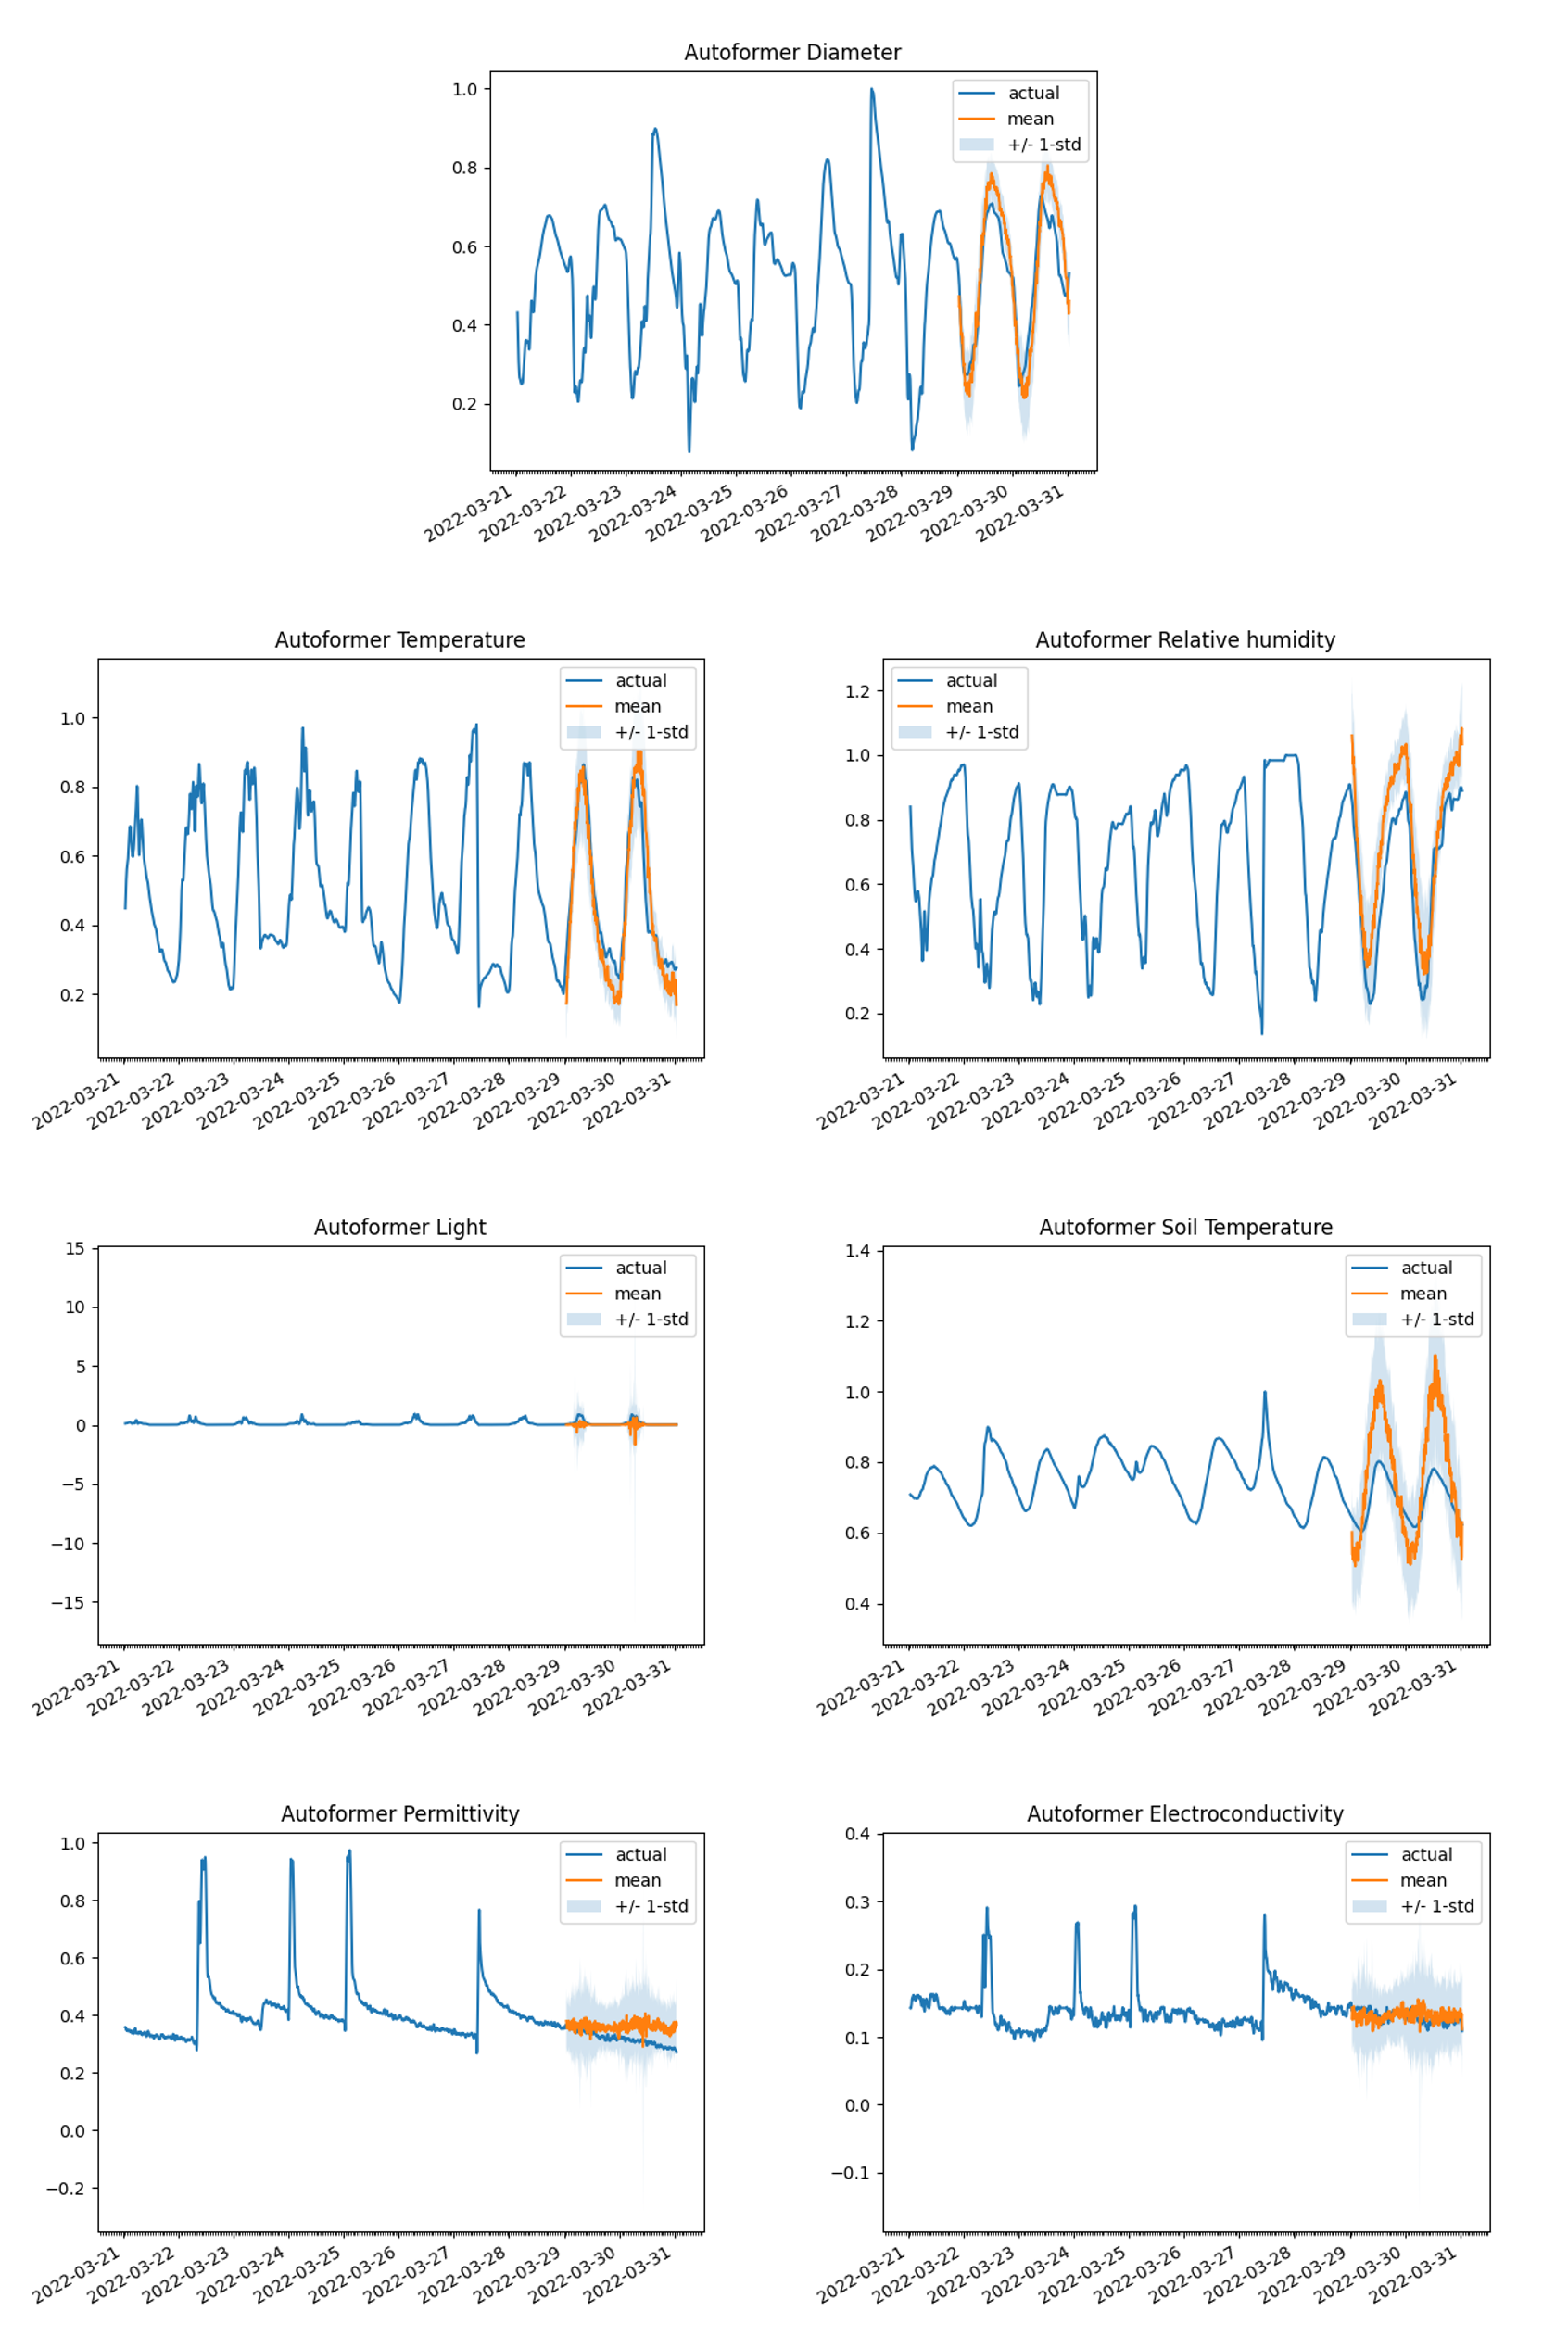
\includegraphics[width=15 cm]{6_ChapterResults/figuras/A29.png}
    \caption{Comparison between the predicted values generated by the A29 model and the actual observed values for the 7 variables over a two-day prediction horizon}
    \label{A29}
\end{figure}
\chapter{Conclusions}\LABCHAP{CAP7}
\pagestyle{esitscCD}

This thesis has explored the use of Transformer architectures, specifically the Vanilla Transformer, Informer, and Autoformer, for time series forecasting. Through our research and experiments, we have gained valuable insights into the strengths and limitations of these models and their relative performance when compared to more traditional methods such as Recurrent Neural Networks (RNN) and Long Short-Term Memory networks (LSTM).

Transformers, as a general architecture, exhibit several notable advantages. They are highly effective at capturing long-term dependencies within data, which is crucial for time series forecasting tasks where understanding patterns over extended periods is essential. Moreover, Transformers are scalable and versatile, allowing them to be adapted to various tasks and data types. However, these benefits come at a cost. Standard Transformer models can be computationally intensive, requiring significant memory and processing power. Additionally, they often need a large amount of data to train effectively, which can be a limitation in situations where data is scarce.

Despite these strengths, our results indicate that the Vanilla Transformer architecture does not perform as well as its more recent counterparts, the Informer and Autoformer, especially considering the trade-offs between computational efficiency and performance. The Informer, in particular, has demonstrated remarkable efficiency, making it the most efficient of the three architectures we examined. This makes it a compelling choice when computational resources are limited or when quick predictions are needed without compromising too much on accuracy.

On the other hand, the Autoformer has shown itself to be the most promising architecture due to its innovative design that specifically targets the forecasting of time series data. However, the improvements in performance were not as significant as anticipated. It is likely that with a different approach to hyperparameter tuning, better results could have been achieved. This suggests that while the Autoformer has a strong foundation, there is room for optimization and improvement in its application to real-world data.

Overall, while these Transformer-based methods did not always surpass traditional methods such as RNNs and LSTMs in our experiments, they demonstrated considerable potential and effectiveness. The ability of Transformers to capture complex, long-range dependencies within time series data suggests that with further research and development, they could potentially outperform current standard methods.

Furthermore, our exploration of multivariate time series forecasting revealed important insights regarding hyperparameter tuning. Specifically, our findings suggest that focusing on optimizing for a single variable can often lead to better performance than attempting to tune hyperparameters for multiple variables simultaneously. This highlights a trade-off between variables, where improving the predictive accuracy for one variable can negatively impact the accuracy for others. This was particularly evident for variables such as electrical conductivity and permittivity, which displayed behavior distinct from other variables, largely due to their dependence on unpredictable factors like rainfall rather than more regular daily or seasonal patterns.

In conclusion, while the Transformer architecture, including its advanced variants like the Informer and Autoformer, offers a promising direction for time series forecasting, there remains a need for further research to optimize their performance fully. This study contributes to the understanding of these models and provides a foundation for future exploration, particularly in refining hyperparameter tuning and exploring how best to leverage the unique strengths of Transformers in different forecasting contexts.

\section{Future Work}

Based on the findings of this thesis, several avenues for future research could further enhance the understanding and application of Transformer architectures for time series forecasting. These directions focus on exploring additional Transformer variants, optimizing hyperparameters more effectively, and deepening the analysis of multivariate time series forecasting.

Firstly, expanding the exploration to include more recent variants of the Transformer architecture, such as SageFormer, InParformer, Stecformer, and SAMformer, could provide valuable insights into how these models compare to the ones studied in this work. Each of these newer models introduces unique modifications and improvements over the original Transformer design, which could potentially address some of the limitations observed in our experiments. For instance, SageFormer and Stecformer are specifically designed to handle sparse data and reduce computational costs, while InParformer and SAMformer offer advanced mechanisms for parallelization and self-attention. Investigating these architectures could not only improve forecasting accuracy but also optimize resource utilization, which is crucial for practical applications.

Another promising direction for future research involves experimenting with various hyperparameter optimization methods. The performance of machine learning models, including Transformers, heavily depends on the choice of hyperparameters, which can significantly influence the model's ability to learn from data and generalize to unseen cases. In this thesis, we primarily utilized a basic approach to hyperparameter tuning, but future studies could benefit from employing more sophisticated techniques such as grid search, random search, Bayesian optimization, gradient-based optimization, and evolutionary optimization. These methods offer different strategies for navigating the hyperparameter space, potentially leading to more optimal configurations and improved model performance. For example, Bayesian optimization uses probabilistic models to predict the performance of different hyperparameter settings, which can efficiently find the best parameters with fewer evaluations compared to random or grid search.

Lastly, there is a substantial opportunity to delve deeper into multivariate time series forecasting. This involves studying how different combinations of input variables affect the forecasting results and understanding the impact of using redundant or irrelevant variables. In our current study, we observed that including certain variables, particularly those that do not have a clear relationship with the target variable, can degrade model performance. Future research could systematically investigate the effects of variable selection on model accuracy and explore techniques for identifying and excluding redundant features. This analysis is crucial, especially in domains where multivariate data can exhibit complex interdependencies, and careful selection of relevant features can lead to more accurate and reliable forecasts.


%% !TEX root =../LibroTipoETSI.tex
\chapter{Transformer}\LABCHAP{CAPEJ}
\pagestyle{esitscCD}

\lettrine[lraise=-0.1, lines=2, loversize=0.25]{E}n este capitulo explicaremos qué es un transformer

\section{What is a Transformer?}

\subsection{Origin and Basic Concept of Transformers}

Transformers were introduced by Vaswani et al. in their seminal 2017 paper titled "Attention is All You Need" \cite{vaswani2023attention}. The primary innovation of the Transformer model is its use of a mechanism called \textit{self-attention} or \textit{scaled dot-product attention}. This allows the model to weigh the importance of different words in a sentence regardless of their position, addressing the limitations of previous recurrent and convolutional neural networks which struggled with long-range dependencies and parallelization.

\subsection{Fundamental Differences from Other Neural Models}

Unlike Recurrent Neural Networks (RNNs) and Long Short-Term Memory networks (LSTMs), which process inputs sequentially, Transformers process the entire sequence of data at once. This parallelization significantly speeds up training and inference times. Additionally, the self-attention mechanism enables the model to capture dependencies between distant words more effectively than RNNs or Convolutional Neural Networks (CNNs), which are limited by their fixed-size receptive fields.

\section{Basic Structure of a Transformer}

\subsection{Attention Mechanism}

The core component of the Transformer architecture is the attention mechanism. It allows the model to focus on different parts of the input sequence when producing each element of the output sequence. The attention mechanism computes a weighted sum of input values (the \textit{values}), with the weights derived from the similarity between a query and corresponding keys. Mathematically, this is expressed as:

\begin{equation}
\text{Attention}(Q, K, V) = \text{softmax}\left(\frac{QK^T}{\sqrt{d_k}}\right)V
\end{equation}

where \( Q \) represents the queries, \( K \) the keys, \( V \) the values, and \( d_k \) the dimensionality of the keys.

\subsection{Encoder and Decoder}

The Transformer architecture consists of two main components: the \textit{encoder} and the \textit{decoder}. 

\par{Encoder:} The encoder is a stack of identical layers, each containing two main sub-layers: a multi-head self-attention mechanism and a position-wise fully connected feed-forward network. Layer normalization and residual connections are employed around each sub-layer to facilitate training.

\par{Decoder:} The decoder is also composed of a stack of identical layers, but with an additional attention sub-layer that attends to the output of the encoder stack. This allows the decoder to condition its predictions on the entire input sequence, not just on the preceding elements of the target sequence.

\subsection{Examples of Applications in Other Fields}

Transformers have found applications beyond their original scope in Natural Language Processing (NLP). They are now widely used in various domains:

\par{Natural Language Processing (NLP):} Models such as BERT \cite{devlin2018bert} and GPT-3 \cite{brown2020language} leverage the Transformer architecture for tasks including language modeling, translation, and text generation.

\par{Computer Vision:} Vision Transformers (ViTs) \cite{dosovitskiy2020image} apply the Transformer architecture to image classification tasks, achieving state-of-the-art performance by treating image patches as sequences of tokens.

\par{Other Fields:} Transformers have also been successfully applied in areas such as audio processing, protein structure prediction \cite{jumper2021highly}, and reinforcement learning, demonstrating the versatility and effectiveness of the model across various types of data and tasks.



%% !TEX root =../LibroTipoETSI.tex
\chapter{Time series Transformer}\LABCHAP{CAPEJ}
\pagestyle{esitscCD}

\section{Overview}

\subsection{Enhancing Time Series Models with Transformers}

Transformers, through their use of multi-head attention, have the potential to significantly enhance time series models' ability to manage long-term dependencies. This approach offers distinct advantages over current methodologies. To illustrate the effectiveness of transformers in handling long-term dependencies, consider how ChatGPT generates extensive and detailed responses in language models. By applying multi-head attention to time series, similar benefits can be achieved: one attention head can concentrate on long-term dependencies, while another focuses on short-term dependencies. This division of attention enables a more comprehensive analysis of the data. Consequently, we believe that transformers could enable time series models to forecast up to 1,000 data points into the future, or possibly even more.

\subsection{The Challenge of Quadratic Complexity}

Transformers face a significant challenge in calculating multi-head self-attention for time series. Since each data point in the series must interact with every other data point, adding more data points exponentially increases the computation time required. This phenomenon, known as quadratic complexity, results in a computational bottleneck when processing lengthy sequences.




%%:Empezamos con los apéndices, que irían en uno o más ficheros. Es necesario incluir estos ficheros entre el entorno \begin{appendices}....\end{appendices} debido a que se ha deseado utilizar un formato diferente para el título de los apéndices, incluyendo la palabra apéndice, para la numeración de los apéndices, alfabético, y para las cabeceras de las páginas.
%
%\begin{appendices}
%
%% Fichero en el que se incluyen los apéndices
%% !TEX root =../LibroTipoETSI.tex



%APENDICE A
\chapter{Codes for Designing Transformer, Informer, and Autoformer Models}\LABAPEN{ApA}
{This appendix provides the Python code utilized for designing and implementing various models discussed in this work, specifically Transformer, Informer, and Autoformer. The included scripts cover different stages of the model development process, including data loading and preprocessing, model definition, training, and evaluation.}
%%%%%%%%%%%%%%%%%
\section{Orchestrator Code}

The main.py script serves as the central execution point for time series forecasting using different model architectures: Transformer, Informer, and Autoformer. The script is structured in a modular manner to facilitate a clear understanding of each step in the forecasting process. Initially, it loads and preprocesses the dataset tailored to the required frequency and prediction length. The script then defines the model architecture based on the chosen model variant and configures the training and backtesting data loaders. The model is trained over a specified number of epochs, leveraging the training data to learn and improve its forecasting capabilities. Once trained, the model's forecasting performance is evaluated on unseen data, and relevant metrics are computed to assess accuracy. Finally, the script generates plots to visually compare the forecasted values with the actual data, offering insights into the model's predictive performance across different variables.

\begin{lstlisting}[language=Python, caption={Code for entry point and orchestration of the time series forecasting pipeline}, breaklines=true, label=code1]

    # %% IMPORT LIBRARIES

    from T1_Load_Dataset import load_and_preprocess_dataset
    from T2_Define_Model import define_my_model
    from T3_Create_DataLoader import create_train_dataloader, create_backtest_dataloader
    from T4_Train_Model import train_model
    from T5_Evaluate_Model import forecasting, see_metrics, plot
    
    # %% DEFINE PARAMETERS
    
    # Select the model variant to use: "Transformer", "Informer", "Autoformer"
    model_variant = "Autoformer"
    
    # Define the frequency of the data sampling and the length of the forecast horizon
    freq = "7min52s"
    prediction_length = 366
    
    # Set the number of epochs for model training
    num_of_epochs = 20
    
    # %% LOAD, SPLIT AND PREPROCESS DATASET
    
    # Load and preprocess the dataset according to the specified frequency and prediction length.
    # The function returns the training and test datasets, the number of variables in the dataset,
    # and the test dataset in its original format for evaluation.
    (multi_variate_train_dataset,
     multi_variate_test_dataset,
     num_of_variates,
     test_dataset) = load_and_preprocess_dataset(freq, prediction_length)
    
    # %% DEFINE THE MODEL
    
    # Define the model architecture based on the selected variant (e.g., Autoformer).
    # The model configuration depends on the number of variables, training data, frequency,
    # and prediction length.
    model = define_my_model(num_of_variates, multi_variate_train_dataset, model_variant, freq, prediction_length)
    
    # %% CREATE DATA LOADERS
    
    # Create a data loader for the training dataset, specifying the batch size and number of batches per epoch.
    # The data loader enables efficient loading of data during training.
    train_dataloader = create_train_dataloader(
        config=model.config,
        freq=freq,
        data=multi_variate_train_dataset,
        batch_size=32,
        num_batches_per_epoch=100,
        num_workers=2,
    )
    
    # Create a data loader for the backtesting dataset to evaluate the model on unseen data.
    test_dataloader = create_backtest_dataloader(
        config=model.config,
        freq=freq,
        data=multi_variate_test_dataset,
        batch_size=32,
    )
    
    # %% TRAIN THE MODEL
    
    # Train the model using the training data loader for the specified number of epochs.
    # The loss function used during training is determined by the model variant.
    train_model(num_of_epochs, model, train_dataloader, model_variant + "_Loss")
    
    # %% FORECASTING AND EVALUATION
    
    # Generate forecasts using the trained model and the test data loader.
    forecasts = forecasting(model, test_dataloader)
    
    # Evaluate the model's performance by calculating relevant metrics and saving them to a file.
    see_metrics(forecasts, test_dataset, prediction_length, freq, "metrics.txt", model_variant + "_Metrics")
    
    # Plot the forecasted and actual values for different variables to visually assess the model's performance.
    plot(forecasts, 0, 0, multi_variate_test_dataset, freq, prediction_length, model_variant + "_Temperature")
    plot(forecasts, 0, 1, multi_variate_test_dataset, freq, prediction_length, model_variant + "_Relative_humidity")
    plot(forecasts, 0, 2, multi_variate_test_dataset, freq, prediction_length, model_variant + "_Light")
    plot(forecasts, 0, 3, multi_variate_test_dataset, freq, prediction_length, model_variant + "_Soil_Temperature")
    plot(forecasts, 0, 4, multi_variate_test_dataset, freq, prediction_length, model_variant + "_Permittivity")
    plot(forecasts, 0, 5, multi_variate_test_dataset, freq, prediction_length, model_variant + "_Electroconductivity")
    plot(forecasts, 0, 6, multi_variate_test_dataset, freq, prediction_length, model_variant + "_Diameter")
    

\end{lstlisting}

\section{Data Preprocessing Code}

The \texttt{T1\_Load\_Dataset.py} script is responsible for the comprehensive loading and preprocessing of time series data, preparing it for use with forecasting models such as Transformers, Informers, and Autoformers. This script consists of two primary functions: \texttt{load\_and\_preprocess\_dataset} and \texttt{load\_my\_own\_dataset}.

The \texttt{load\_and\_preprocess\_dataset} function coordinates the conversion of raw data into a format suitable for multivariate time series forecasting. It begins by calling \texttt{load\_my\_own\_dataset} to read and preprocess the data. Subsequent transformations are applied, including handling missing values, detrending, and smoothing. After normalization, the data is split into training, validation, and test sets. These datasets are then reformatted using GluonTS tools, which are essential for time series modeling.

The \texttt{load\_my\_own\_dataset} function performs specific tasks related to data loading and initial preprocessing. It reads the dataset from a CSV file, selects relevant features, removes missing values, and applies trend removal techniques. It also normalizes the data and splits it into training, validation, and test subsets. Additionally, this function includes visualization steps to evaluate the quality of the data and the effects of preprocessing.



\begin{lstlisting}[language=Python, caption={Code for loading and preprocessing the time series data}, breaklines=true, label=code2]

    # %% LIBRARIES

    from gluonts.dataset.multivariate_grouper import MultivariateGrouper
    from functools import partial, lru_cache
    import pandas as pd
    import matplotlib.pyplot as plt
    import os
    from scipy.signal import savgol_filter
    from datasets import Dataset
    from sklearn.preprocessing import MinMaxScaler
    import matplotlib.dates as mdates
    import numpy as np

    # %% LOAD AND PREPROCESS DATASET FUNCTION

    def load_and_preprocess_dataset(freq, prediction_length):
    """
    Loads and preprocesses the dataset, then converts it into a multivariate time series
    suitable for training and testing forecasting models.

    Parameters:
    - freq (str): The frequency of data points in the dataset (e.g., '7min52s').
    - prediction_length (int): The number of time steps to predict.

    Returns:
    - tuple: Contains the multivariate training dataset, multivariate testing dataset,
                the number of variables, and the original test dataset.
    """

    # Load custom dataset using a helper function
    validationtest_dataset, test_dataset, train_dataset = load_my_own_dataset(prediction_length)

    # Cache for converting date to pandas period
    @lru_cache(maxsize=10_000)
    def convert_to_pandas_period(date, freq):
        return pd.Period(date, freq)

    # Transform function for dataset start field
    def transform_start_field(batch, freq):
        batch["start"] = [convert_to_pandas_period(date, freq) for date in batch["start"]]
        return batch

    # Apply the transformation to datasets
    train_dataset.set_transform(partial(transform_start_field, freq=freq))
    test_dataset.set_transform(partial(transform_start_field, freq=freq))

    # Determine the number of variables in the dataset
    num_of_variates = len(train_dataset)

    # Group datasets for multivariate time series forecasting
    train_grouper = MultivariateGrouper(max_target_dim=num_of_variates)
    test_grouper = MultivariateGrouper(max_target_dim=num_of_variates, num_test_dates=len(test_dataset) // num_of_variates)

    # Transform datasets into multivariate format
    multi_variate_train_dataset = train_grouper(train_dataset)
    multi_variate_test_dataset = test_grouper(test_dataset)

    return multi_variate_train_dataset, multi_variate_test_dataset, num_of_variates, test_dataset

    # %% LOAD CUSTOM DATASET FROM CSV FUNCTION

    def load_my_own_dataset(prediction_length):
    """
    Loads and preprocesses the custom dataset from a CSV file, normalizes the data, 
    and splits it into training, validation, and testing datasets.

    Parameters:
    - prediction_length (int): The number of time steps to predict.

    Returns:
    - tuple: Contains the validation, test, and training datasets in GluonTS format.
    """

    # Construct the file path to the dataset
    current_path = os.path.dirname(os.path.abspath(__file__))
    directory_name = 'Create_2024_dataset'
    file_name = 'Clay_2.csv'
    file_path = os.path.join(current_path, directory_name, file_name)

    # Load the dataset into a pandas DataFrame
    df = pd.read_csv(file_path, sep=";")

    # Select relevant variables for forecasting
    data = df[['Temperature', 'Relative_humidity', 'Light', 'Soil_temperature',
                'Permittivity', 'Electroconductivity', 'Diameter']]

    # Remove rows with NaN values
    index_nan = data[data.isna().any(axis=1)].index
    data = data.dropna()

    # Detrend data by removing the rolling mean
    window_value = 100
    for col in ['Diameter']:
        data.loc[:, col] = data[col] - data[col].rolling(window=window_value).mean()

    # Drop rows with NaN values created by detrending
    data = data.dropna()

    # Visualize the distribution of eliminated data points
    plt.figure(figsize=(10, 2))
    plt.plot(index_nan, np.ones_like(index_nan), 'ro', markersize=2)
    plt.title(f'Nan index distribution. \n Number of eliminated measurements: {len(index_nan)}')
    plt.xlabel('Index')
    plt.ylabel('Frequency')
    plt.yticks([])
    plt.grid(True)
    plt.xlim(0, len(df))
    plt.show()

    # Smooth the data using Savitzky-Golay filter
    for col in data.columns:
        data[col] = savgol_filter(data[col], 11, 2)

    # Convert date column to datetime and calculate the sampling period
    dates = pd.to_datetime(df['Date'].drop(index_nan))
    intervals = dates.diff()
    sampling_period = intervals.mean()
    print("\nAverage sampling period:\n", sampling_period)

    # Normalize the data using Min-Max Scaler
    scaler = MinMaxScaler()
    scaled_data = scaler.fit_transform(data)
    data[data.columns] = scaled_data

    # Split data into training, validation, and test sets
    data_test = data
    data_validation = data.iloc[:-prediction_length]
    data_train = data.iloc[:-2 * prediction_length]

    # Prepare datasets for GluonTS
    dict_validation = {'start': [], 'target': [], 'feat_static_cat': [], 'feat_dynamic_real': [], 'item_id': []}
    dict_test = {'start': [], 'target': [], 'feat_static_cat': [], 'feat_dynamic_real': [], 'item_id': []}
    dict_train = {'start': [], 'target': [], 'feat_static_cat': [], 'feat_dynamic_real': [], 'item_id': []}

    # Populate dictionaries with data for GluonTS
    for i in range(1, 8):
        dict_validation['target'].append(data_validation.iloc[:, i-1].values.astype('float32'))
        dict_test['target'].append(data_test.iloc[:, i-1].values.astype('float32'))
        dict_train['target'].append(data_train.iloc[:, i-1].values.astype('float32'))

        for d in [dict_validation, dict_test, dict_train]:
            d['start'].append(pd.Timestamp('2022-01-01 13:14:26'))
            d['feat_static_cat'].append(i)
            d['feat_dynamic_real'].append(None)
            d['item_id'].append(f'T{i}')

    # Convert dictionaries to GluonTS datasets
    dataset_validation = Dataset.from_pandas(pd.DataFrame(dict_validation))
    dataset_test = Dataset.from_pandas(pd.DataFrame(dict_test))
    dataset_train = Dataset.from_pandas(pd.DataFrame(dict_train))

    # Visualize training and test data
    plot_dataset(train_dataset=dataset_train, test_dataset=dataset_test, data=data, prediction_length=prediction_length)

    return dataset_validation, dataset_test, dataset_train

    # %% HELPER FUNCTION TO PLOT DATASETS

    def plot_dataset(train_dataset, test_dataset, data, prediction_length):
    """
    Plots the training and test datasets to visualize the time series data used for forecasting.

    Parameters:
    - train_dataset (Dataset): The training dataset in GluonTS format.
    - test_dataset (Dataset): The test dataset in GluonTS format.
    - data (pd.DataFrame): The original data used for forecasting.
    - prediction_length (int): The number of time steps to predict.
    """

    start_date = "2022-01-01"
    frequency = '7min52s'

    def generate_dates(start, num_periods, freq):
        return pd.date_range(start=start, periods=num_periods, freq=freq)

    for var in range(7):
        num_periods_train = len(train_dataset[var]["target"])
        num_periods_test = len(test_dataset[var]["target"])

        train_dates = generate_dates(start_date, num_periods_train, frequency)
        test_dates = generate_dates(start_date, num_periods_test, frequency)

        # Plot full data
        plt.figure(figsize=(20, 6.4))
        plt.plot(train_dates, train_dataset[var]["target"], color="blue", label="Train")
        plt.plot(test_dates[-2*prediction_length:], test_dataset[var]["target"][-2*prediction_length:], color="red", label="Test")
        plt.title(data.columns[var].replace('_', ' '))
        plt.legend()
        plt.xticks(rotation=30, ha='right')
        plt.gca().xaxis.set_major_formatter(mdates.DateFormatter('%Y-%m-%d'))
        plt.show()

        # Plot zoomed segment
        plt.figure()
        plt.plot(train_dates[-3*prediction_length:], train_dataset[var]["target"][-3*prediction_length:], color="blue", label="Train (zoom)")
        plt.plot(test_dates[-2*prediction_length:], test_dataset[var]["target"][-2*prediction_length:], color="red", label="Test (zoom)")
        plt.title(data.columns[var].replace('_', ' '))
        plt.legend()
        plt.xticks(rotation=30, ha='right')
        plt.gca().xaxis.set_major_formatter(mdates.DateFormatter('%Y-%m-%d'))
        plt.show()
    

\end{lstlisting}

\section{Model Definition Code}

The \texttt{define\_my\_model} function is designed to create and configure a time series forecasting model based on the specified variant: "Transformer", "Informer", or "Autoformer". The function takes several parameters, including the number of variates in the time series, the dataset, the chosen model variant, the frequency of the time series data, and the prediction length.

Firstly, the function retrieves default lag values and time features based on the given frequency using GluonTS utilities. It then configures the model according to the selected variant.

If an invalid model variant is provided, the function raises a \texttt{ValueError}. The function returns the configured model instance, ready for training and evaluation. This approach ensures that the model architecture is tailored to the specific needs of the time series data and forecasting task.

\begin{lstlisting}[language=Python, caption={Code for defining the architecture and hyperparameters of the forecasting model}, breaklines=true, label=code3]

    # %% LIBRARIES

    from transformers import InformerConfig, InformerForPrediction
    from transformers import AutoformerConfig, AutoformerForPrediction
    from transformers import TimeSeriesTransformerConfig, TimeSeriesTransformerForPrediction
    from gluonts.time_feature import time_features_from_frequency_str, get_lags_for_frequency
    import pandas as pd
    
    # %% DEFINE MODEL
    
    def define_my_model(num_of_variates, multi_variate_train_dataset, model_variant, freq, prediction_length):
        """
        Defines and returns a time series forecasting model based on the specified variant.
        
        Parameters:
        - num_of_variates (int): Number of variables in the time series data.
        - multi_variate_train_dataset (Dataset): Training dataset in a multivariate format.
        - model_variant (str): Type of model to define. Options are "Transformer", "Informer", or "Autoformer".
        - freq (str): Frequency of the time series data (e.g., '7min52s').
        - prediction_length (int): Length of the prediction horizon.
        
        Returns:
        - model (Model): Configured model instance for forecasting.
        """
        
        # Get default lags and time features based on the frequency
        lags_sequence = get_lags_for_frequency(freq)
        time_features = time_features_from_frequency_str(freq)
    
        # Define model configuration based on the specified model variant
        if model_variant == "Transformer":
            config = TimeSeriesTransformerConfig(
                input_size=num_of_variates,
                prediction_length=prediction_length,
                context_length=prediction_length * 2,
                lags_sequence=[
                    1, 2, 3, 4, 5, 183 + 1, 183 + 2, 183 + 3, 183 + 4, 183 + 5,
                    366 + 1, 366 + 2, 366 + 3, 366 + 4, 366 + 5, 549 + 1, 549 + 2,
                    549 + 3, 549 + 4, 549 + 5
                ],
                num_time_features=len(time_features) + 1,
                dropout=0.2,
                encoder_layers=4,
                decoder_layers=4,
                d_model=32,
            )
            model = TimeSeriesTransformerForPrediction(config)
    
        elif model_variant == "Informer":
            config = InformerConfig(
                input_size=num_of_variates,
                prediction_length=prediction_length,
                context_length=prediction_length * 2,
                lags_sequence=[
                    1, 2, 3, 4, 5, 183 + 1, 183 + 2, 183 + 3, 183 + 4, 183 + 5,
                    366 + 1, 366 + 2, 366 + 3, 366 + 4, 366 + 5, 549 + 1, 549 + 2,
                    549 + 3, 549 + 4, 549 + 5
                ],
                num_time_features=len(time_features) + 1,
                dropout=0.1,
                encoder_layers=4,
                decoder_layers=4,
                d_model=32,
            )
            model = InformerForPrediction(config)
    
        elif model_variant == "Autoformer":
            config = AutoformerConfig(
                input_size=num_of_variates,
                prediction_length=prediction_length,
                context_length=prediction_length * 2,
                lags_sequence=lags_sequence,
                num_time_features=len(time_features) + 1,
                dropout=0.1,
                encoder_layers=6,
                decoder_layers=4,
                d_model=64,
            )
            model = AutoformerForPrediction(config)
    
        else:
            raise ValueError("ERROR: No valid model variant specified. Choose 'Transformer', 'Informer', or 'Autoformer'.")
    
        return model
    

\end{lstlisting}

\section{Data Loader Creation Code}

The provided code defines functions for creating data loaders for training, backtesting, and testing time series models using the GluonTS library. These functions preprocess time series data according to the model's configuration and the specific mode of operation.

\begin{itemize}
    \item \texttt{create\_train\_dataloader}: Prepares and transforms training data by applying necessary transformations and splitting it into batches. It also supports caching and shuffling of data.
    \item \texttt{create\_backtest\_dataloader}: Configures a data loader for backtesting purposes, focusing on validation data.
    \item \texttt{create\_test\_dataloader}: Sets up a data loader for testing, processing data for evaluation on unseen samples.
\end{itemize}

The \texttt{create\_instance\_splitter} function creates an instance splitter based on the mode (train, validation, or test), which partitions the time series data into instances suitable for model training or evaluation. The \texttt{create\_transformation} function generates a transformation pipeline that preprocesses the data, including handling missing values, adding time-based features, and renaming fields to match the expected input format.

These functions ensure that the data is properly formatted and split for model training, validation, and testing, facilitating effective model evaluation and performance monitoring.

\begin{lstlisting}[language=Python, caption={Code for creating data loaders for efficient training and evaluation}, breaklines=true, label=code4]

    # %% LIBRARIES

    from typing import Iterable, Optional
    from transformers import PretrainedConfig
    import torch
    from gluonts.itertools import Cached, Cyclic
    from gluonts.dataset.loader import as_stacked_batches
    from gluonts.time_feature import time_features_from_frequency_str, TimeFeature, get_lags_for_frequency
    from gluonts.dataset.field_names import FieldName
    from gluonts.transform import (
        AddAgeFeature,
        AddObservedValuesIndicator,
        AddTimeFeatures,
        AsNumpyArray,
        Chain,
        ExpectedNumInstanceSampler,
        InstanceSplitter,
        RemoveFields,
        SelectFields,
        SetField,
        TestSplitSampler,
        Transformation,
        ValidationSplitSampler,
        VstackFeatures,
        RenameFields,
    )
    from gluonts.transform.sampler import InstanceSampler
    
    
    def create_train_dataloader(
        config: PretrainedConfig,
        freq: str,
        data,
        batch_size: int,
        num_batches_per_epoch: int,
        shuffle_buffer_length: Optional[int] = None,
        cache_data: bool = True,
        **kwargs,
    ) -> Iterable:
        """
        Creates a data loader for training.
    
        Parameters:
            config (PretrainedConfig): Configuration for the model.
            freq (str): Frequency of the time series data.
            data: Input data for training.
            batch_size (int): Size of each batch.
            num_batches_per_epoch (int): Number of batches per epoch.
            shuffle_buffer_length (Optional[int]): Buffer length for shuffling the data.
            cache_data (bool): Whether to cache the data.
    
        Returns:
            Iterable: A data loader for training.
        """
        # Define input names based on configuration
        prediction_input_names = [
            "past_time_features",
            "past_values",
            "past_observed_mask",
            "future_time_features",
        ]
        if config.num_static_categorical_features > 0:
            prediction_input_names.append("static_categorical_features")
        if config.num_static_real_features > 0:
            prediction_input_names.append("static_real_features")
    
        training_input_names = prediction_input_names + [
            "future_values",
            "future_observed_mask",
        ]
    
        # Create and apply transformations
        transformation = create_transformation(freq, config)
        transformed_data = transformation.apply(data, is_train=True)
        if cache_data:
            transformed_data = Cached(transformed_data)
    
        # Initialize the instance splitter for training
        instance_splitter = create_instance_splitter(config, "train")
        stream = Cyclic(transformed_data).stream()
        training_instances = instance_splitter.apply(stream)
    
        return as_stacked_batches(
            training_instances,
            batch_size=batch_size,
            shuffle_buffer_length=shuffle_buffer_length,
            field_names=training_input_names,
            output_type=torch.tensor,
            num_batches_per_epoch=num_batches_per_epoch,
        )
    
    
    def create_backtest_dataloader(
        config: PretrainedConfig,
        freq: str,
        data,
        batch_size: int,
        **kwargs,
    ) -> Iterable:
        """
        Creates a data loader for backtesting.
    
        Parameters:
            config (PretrainedConfig): Configuration for the model.
            freq (str): Frequency of the time series data.
            data: Input data for backtesting.
            batch_size (int): Size of each batch.
    
        Returns:
            Iterable: A data loader for backtesting.
        """
        prediction_input_names = [
            "past_time_features",
            "past_values",
            "past_observed_mask",
            "future_time_features",
        ]
        if config.num_static_categorical_features > 0:
            prediction_input_names.append("static_categorical_features")
        if config.num_static_real_features > 0:
            prediction_input_names.append("static_real_features")
    
        # Create and apply transformations
        transformation = create_transformation(freq, config)
        transformed_data = transformation.apply(data)
    
        # Initialize the instance splitter for validation
        instance_sampler = create_instance_splitter(config, "validation")
        testing_instances = instance_sampler.apply(transformed_data, is_train=True)
    
        return as_stacked_batches(
            testing_instances,
            batch_size=batch_size,
            output_type=torch.tensor,
            field_names=prediction_input_names,
        )
    
    
    def create_test_dataloader(
        config: PretrainedConfig,
        freq: str,
        data,
        batch_size: int,
        **kwargs,
    ) -> Iterable:
        """
        Creates a data loader for testing.
    
        Parameters:
            config (PretrainedConfig): Configuration for the model.
            freq (str): Frequency of the time series data.
            data: Input data for testing.
            batch_size (int): Size of each batch.
    
        Returns:
            Iterable: A data loader for testing.
        """
        prediction_input_names = [
            "past_time_features",
            "past_values",
            "past_observed_mask",
            "future_time_features",
        ]
        if config.num_static_categorical_features > 0:
            prediction_input_names.append("static_categorical_features")
        if config.num_static_real_features > 0:
            prediction_input_names.append("static_real_features")
    
        # Create and apply transformations
        transformation = create_transformation(freq, config)
        transformed_data = transformation.apply(data, is_train=False)
    
        # Initialize the instance splitter for testing
        instance_sampler = create_instance_splitter(config, "test")
        testing_instances = instance_sampler.apply(transformed_data, is_train=False)
    
        return as_stacked_batches(
            testing_instances,
            batch_size=batch_size,
            output_type=torch.tensor,
            field_names=prediction_input_names,
        )
    
    
    def create_instance_splitter(
        config: PretrainedConfig,
        mode: str,
        train_sampler: Optional[InstanceSampler] = None,
        validation_sampler: Optional[InstanceSampler] = None,
    ) -> Transformation:
        """
        Creates an instance splitter for different modes (train, validation, test).
    
        Parameters:
            config (PretrainedConfig): Configuration for the model.
            mode (str): Mode for the instance splitter ("train", "validation", "test").
            train_sampler (Optional[InstanceSampler]): Custom sampler for training.
            validation_sampler (Optional[InstanceSampler]): Custom sampler for validation.
    
        Returns:
            Transformation: An instance splitter transformation.
        """
        assert mode in ["train", "validation", "test"], "Invalid mode specified"
    
        instance_sampler = {
            "train": train_sampler or ExpectedNumInstanceSampler(
                num_instances=1.0, min_future=config.prediction_length
            ),
            "validation": validation_sampler or ValidationSplitSampler(min_future=config.prediction_length),
            "test": TestSplitSampler(),
        }[mode]
    
        return InstanceSplitter(
            target_field="values",
            is_pad_field=FieldName.IS_PAD,
            start_field=FieldName.START,
            forecast_start_field=FieldName.FORECAST_START,
            instance_sampler=instance_sampler,
            past_length=config.context_length + max(config.lags_sequence),
            future_length=config.prediction_length,
            time_series_fields=["time_features", "observed_mask"],
        )
    
    
    def create_transformation(freq: str, config: PretrainedConfig) -> Transformation:
        """
        Creates a transformation pipeline for data preprocessing.
    
        Parameters:
            freq (str): Frequency of the time series data.
            config (PretrainedConfig): Configuration for the model.
    
        Returns:
            Transformation: A transformation pipeline.
        """
        remove_field_names = []
        if config.num_static_real_features == 0:
            remove_field_names.append(FieldName.FEAT_STATIC_REAL)
        if config.num_dynamic_real_features == 0:
            remove_field_names.append(FieldName.FEAT_DYNAMIC_REAL)
        if config.num_static_categorical_features == 0:
            remove_field_names.append(FieldName.FEAT_STATIC_CAT)
    
        return Chain(
            [
                RemoveFields(field_names=remove_field_names),
            ]
            + (
                [AsNumpyArray(
                    field=FieldName.FEAT_STATIC_CAT,
                    expected_ndim=1,
                    dtype=int,
                )]
                if config.num_static_categorical_features > 0
                else []
            )
            + (
                [AsNumpyArray(
                    field=FieldName.FEAT_STATIC_REAL,
                    expected_ndim=1,
                )]
                if config.num_static_real_features > 0
                else []
            )
            + [
                AsNumpyArray(
                    field=FieldName.TARGET,
                    expected_ndim=1 if config.input_size == 1 else 2,
                ),
                AddObservedValuesIndicator(
                    target_field=FieldName.TARGET,
                    output_field=FieldName.OBSERVED_VALUES,
                ),
                AddTimeFeatures(
                    start_field=FieldName.START,
                    target_field=FieldName.TARGET,
                    output_field=FieldName.FEAT_TIME,
                    time_features=time_features_from_frequency_str(freq),
                    pred_length=config.prediction_length,
                ),
                AddAgeFeature(
                    target_field=FieldName.TARGET,
                    output_field=FieldName.FEAT_AGE,
                    pred_length=config.prediction_length,
                    log_scale=True,
                ),
                VstackFeatures(
                    output_field=FieldName.FEAT_TIME,
                    input_fields=[FieldName.FEAT_TIME, FieldName.FEAT_AGE]
                    + (
                        [FieldName.FEAT_DYNAMIC_REAL]
                        if config.num_dynamic_real_features > 0
                        else []
                    ),
                ),
                RenameFields(
                    mapping={
                        FieldName.FEAT_STATIC_CAT: "static_categorical_features",
                        FieldName.FEAT_STATIC_REAL: "static_real_features",
                        FieldName.FEAT_TIME: "time_features",
                        FieldName.TARGET: "values",
                        FieldName.OBSERVED_VALUES: "observed_mask",
                    }
                ),
            ]
        )
    

\end{lstlisting}

\section{Model Training Code}

The \texttt{train\_model} function is responsible for training a deep learning model using the provided training data. It utilizes the \texttt{Accelerator} from the Hugging Face \texttt{accelerate} library to manage distributed and mixed precision training, making the process more efficient.

The function accepts the number of epochs, the model to be trained, a data loader for the training data, and a title for saving outputs. It initializes the model and optimizer, and then enters a training loop where it performs forward and backward passes to update model parameters. The training loss is recorded and printed periodically.

After training, the function calculates the total training time and prints it. It also saves the training time to a text file and plots the loss history over iterations, saving the plot as an image file. This approach allows for monitoring the training process and evaluating the model's performance visually.

\begin{lstlisting}[language=Python, caption={Code for training the forecasting model}, breaklines=true, label=code5]

    # %% LIBRARIES

    from accelerate import Accelerator
    from torch.optim import AdamW
    import matplotlib.pyplot as plt
    import numpy as np
    import os
    import time
    
    def train_model(num_of_epochs, model, train_dataloader, title):
        """
        Trains a given model using the provided training data loader and saves the training loss over iterations.
        
        Parameters:
        - num_of_epochs (int): Number of epochs to train the model.
        - model (torch.nn.Module): The model to be trained.
        - train_dataloader (DataLoader): DataLoader instance for the training data.
        - title (str): Title used to name the saved plot and text file.
        
        Returns:
        - model (torch.nn.Module): The trained model.
        """
        
        epochs = num_of_epochs
        loss_history = []
    
        # Initialize Accelerator for distributed and mixed precision training
        accelerator = Accelerator()
        device = accelerator.device
    
        # Move the model to the appropriate device
        model.to(device)
        optimizer = AdamW(model.parameters(), lr=6e-4, betas=(0.9, 0.95), weight_decay=1e-1)
    
        # Prepare model, optimizer, and dataloader for distributed training
        model, optimizer, train_dataloader = accelerator.prepare(model, optimizer, train_dataloader)
    
        model.train()
        
        # Record start time
        start_time = time.time()
    
        # Training loop
        for epoch in range(epochs):
            for idx, batch in enumerate(train_dataloader):
                optimizer.zero_grad()
                outputs = model(
                    static_categorical_features=batch["static_categorical_features"].to(device) if model.config.num_static_categorical_features > 0 else None,
                    static_real_features=batch["static_real_features"].to(device) if model.config.num_static_real_features > 0 else None,
                    past_time_features=batch["past_time_features"].to(device),
                    past_values=batch["past_values"].to(device),
                    future_time_features=batch["future_time_features"].to(device),
                    future_values=batch["future_values"].to(device),
                    past_observed_mask=batch["past_observed_mask"].to(device),
                    future_observed_mask=batch["future_observed_mask"].to(device),
                )
                loss = outputs.loss
    
                # Backpropagation and optimization
                accelerator.backward(loss)
                optimizer.step()
    
                loss_history.append(loss.item())
                if idx % 100 == 0:
                    print(f"Iteration {idx}: Loss = {loss.item()}")
    
        # Calculate and print the total training time
        end_time = time.time()
        training_time = end_time - start_time
        print(f"\nTraining time: {training_time:.2f} seconds\n")
    
        # Ensure the 'plots' directory exists
        plots_folder = "plots"
        if not os.path.exists(plots_folder):
            os.makedirs(plots_folder)
    
        # Save the training time to a text file
        output_file = os.path.join(plots_folder, "training_time.txt")
        with open(output_file, "w") as f:
            f.write(f"Training time for '{title}': {training_time:.2f} seconds")
    
        # Plot the loss history
        loss_history = np.array(loss_history)
        plt.figure(figsize=(10, 5))
        plt.plot(loss_history, label="Training Loss")
        plt.title("Training Loss over Iterations", fontsize=15)
        plt.xlabel("Iteration")
        plt.ylabel("Loss")
        plt.legend(loc="upper right")
    
        # Save the plot
        filename = os.path.join(plots_folder, title.replace(" ", "_") + ".png")
        plt.savefig(filename)
        print("Plot saved as:", filename)
    
        plt.show()
    
        return model
    

\end{lstlisting}

\section{Model Evaluation Code}

The provided code includes functions to generate forecasts, evaluate model performance, and visualize results for time series forecasting tasks.

\begin{itemize}
    \item \texttt{forecasting}: This function uses a trained model to generate forecasts for a given test dataloader. It moves data to the appropriate device (GPU/CPU) and accumulates forecasts from the model into a NumPy array.
    
    \item \texttt{see\_metrics}: Computes performance metrics for the forecasts, such as Mean Squared Error (MSE) and R-squared, using the `evaluate` library. It writes these metrics to a file and creates a scatter plot to visualize the relationship between MSE and R-squared values. Metrics are computed for each time series in the test dataset, and results are saved in a specified directory.
    
    \item \texttt{plot}: Generates a plot comparing the actual values of a time series against the model’s forecasts. It visualizes both the mean forecast and the uncertainty bounds (plus/minus one standard deviation). The plot is saved to a file and includes time series data with appropriate labels and formatting.
\end{itemize}

These functions facilitate model evaluation and result interpretation, providing both numerical metrics and visual insights into the forecasting performance.

\begin{lstlisting}[language=Python, caption={Code for evaluating the model’s performance}, breaklines=true, label=code6]

    # %% LIBRARIES

    import matplotlib.dates as mdates
    from evaluate import load
    import math
    from accelerate import Accelerator
    import matplotlib.pyplot as plt
    import numpy as np
    import pandas as pd
    from gluonts.dataset.field_names import FieldName
    import os
    
    def forecasting(model, test_dataloader):
        """
        Generates forecasts using the provided model and test dataloader.
    
        Parameters:
        - model: The trained forecasting model.
        - test_dataloader: DataLoader providing the test data.
    
        Returns:
        - forecasts: Numpy array of generated forecasts.
        """
        accelerator = Accelerator()
        device = accelerator.device
        model.eval()
    
        forecasts = []
    
        for batch in test_dataloader:
            outputs = model.generate(
                static_categorical_features=batch["static_categorical_features"].to(device)
                if model.config.num_static_categorical_features > 0
                else None,
                static_real_features=batch["static_real_features"].to(device)
                if model.config.num_static_real_features > 0
                else None,
                past_time_features=batch["past_time_features"].to(device),
                past_values=batch["past_values"].to(device),
                future_time_features=batch["future_time_features"].to(device),
                past_observed_mask=batch["past_observed_mask"].to(device),
            )
            forecasts.append(outputs.sequences.cpu().numpy())
    
        forecasts = np.vstack(forecasts)
    
        return forecasts
    
    def see_metrics(forecasts, test_dataset, prediction_length, freq, output_file, title):
        """
        Computes and visualizes metrics for the forecasts and saves the results to a file.
    
        Parameters:
        - forecasts: Numpy array of forecasted values.
        - test_dataset: The test dataset containing ground truth values.
        - prediction_length: Number of time steps to predict.
        - freq: Frequency of the time series data.
        - output_file: Path to the output file where metrics will be saved.
        - title: Title for the resulting plot.
        """
        mse_metric = load("evaluate-metric/mse")
        r_squared_metric = load("evaluate-metric/r_squared")
    
        forecast_median = np.median(forecasts, 1).squeeze(0).T
    
        mse_metrics = []
        r_squared_metrics = []
    
        plots_folder = "plots"
        if not os.path.exists(plots_folder):
            os.makedirs(plots_folder)
    
        output_file = os.path.join(plots_folder, output_file)
        with open(output_file, 'w') as f:
            f.write("\t\t\tMSE\t\t\tR_squared\n")
    
            for item_id, ts in enumerate(test_dataset):
                ground_truth = ts["target"][-prediction_length:]
    
                mse = mse_metric.compute(
                    predictions=forecast_median[item_id],
                    references=np.array(ground_truth))
                mse['mse'] = 10 * math.log10(mse['mse'])
    
                r_squared = r_squared_metric.compute(
                    predictions=forecast_median[item_id],
                    references=np.array(ground_truth))
    
                mse_metrics.append(mse['mse'])
                r_squared_metrics.append(r_squared)
    
                if item_id == 0:
                    f.write(f"Temperature\t\t{mse['mse']:.6f}\t\t{r_squared:.6f}\n")
                elif item_id == 1:
                    f.write(f"Relative_humidity\t{mse['mse']:.6f}\t\t{r_squared:.6f}\n")
                elif item_id == 2:
                    f.write(f"Light\t\t\t{mse['mse']:.6f}\t\t{r_squared:.6f}\n")
                elif item_id == 3:
                    f.write(f"Soil_Temperature\t{mse['mse']:.6f}\t\t{r_squared:.6f}\n")
                elif item_id == 4:
                    f.write(f"Permittivity\t\t{mse['mse']:.6f}\t\t{r_squared:.6f}\n")
                elif item_id == 5:
                    f.write(f"Electroconductivity\t{mse['mse']:.6f}\t\t{r_squared:.6f}\n")
                elif item_id == 6:
                    f.write(f"Diameter\t\t{mse['mse']:.6f}\t\t{r_squared:.6f}\n")
    
        plt.scatter(mse_metrics, r_squared_metrics, alpha=0.2)
        plt.xlabel("MSE")
        plt.ylabel("R-squared")
    
        filename = os.path.join(plots_folder, title.replace(" ", "_") + ".png")
        plt.savefig(filename)
        print("Image saved as:", filename)
        plt.show()
    
    def plot(forecasts, ts_index, mv_index, multi_variate_test_dataset, freq, prediction_length, title):
        """
        Plots the forecasts against actual values for a specified time series.
    
        Parameters:
        - forecasts: Numpy array of forecasted values.
        - ts_index: Index of the time series to plot.
        - mv_index: Index of the multivariate time series component to plot.
        - multi_variate_test_dataset: The test dataset containing time series data.
        - freq: Frequency of the time series data.
        - prediction_length: Number of time steps to predict.
        - title: Title for the plot.
        """
        fig, ax = plt.subplots()
    
        index = pd.period_range(
            start=multi_variate_test_dataset[ts_index][FieldName.START],
            periods=len(multi_variate_test_dataset[0][FieldName.TARGET][0]),
            freq=multi_variate_test_dataset[ts_index][FieldName.START].freq,
        ).to_timestamp()
    
        ax.xaxis.set_minor_locator(mdates.HourLocator())
    
        ax.plot(
            index[-5 * prediction_length:],
            multi_variate_test_dataset[ts_index]["target"][mv_index, -5 * prediction_length:],
            label="Actual",
        )
    
        ax.plot(
            index[-prediction_length:],
            forecasts[ts_index, ..., mv_index].mean(axis=0),
            label="Mean Forecast",
        )
    
        ax.fill_between(
            index[-prediction_length:],
            forecasts[ts_index, ..., mv_index].mean(0) - forecasts[ts_index, ..., mv_index].std(axis=0),
            forecasts[ts_index, ..., mv_index].mean(0) + forecasts[ts_index, ..., mv_index].std(axis=0),
            alpha=0.2,
            interpolate=True,
            label="+/- 1-std",
        )
        ax.legend()
        ax.set_title(title.replace("_", " "))
        fig.autofmt_xdate()
    
        plots_folder = "plots"
        if not os.path.exists(plots_folder):
            os.makedirs(plots_folder)
    
        filename = os.path.join(plots_folder, title.replace(" ", "_") + ".png")
        plt.savefig(filename)
        print("Image saved as:", filename)
    
        plt.show()
    

\end{lstlisting} %Ver este fichero para incluir ahí los apéndices.
%
%\end{appendices}
%:Fin de la inclusión de apéndices

%:Empieza todo lo que no constituye el cuerpo en si del libro. Todo lo que va detrás
\backmatter

%:Indice de figuras, coméntese las siguientes líneas si no se desea
\cleardoublepage
\phantomsection

%:Para añadir una línea en blanco en el TOC y separar esta lista
\addtocontents{toc}{\protect\mbox{}\protect\hspace*{0pt}\par}
\addcontentsline{toc}{listasb}{\listfigurename}
\pagestyle{especial}
\listoffigures

%:Indice de tablas, coméntese las siguientes líneas si no se desea
\cleardoublepage
\phantomsection
\addcontentsline{toc}{listasb}{\listtablename}
\pagestyle{especial}
\listoftables

%:Indice de Programas
\cleardoublepage
\phantomsection
\addcontentsline{toc}{listasb}{\lstlistlistingname}
\pagestyle{especial}
\lstlistoflistings

%:Bibliografía con biblatex y biber
\cleardoublepage
\phantomsection
\addcontentsline{toc}{listasb}{\bibname}
\pagestyle{especial}
%BIBER
%\printbibliography[heading=etsi]
%BIBTEX
\bibliographystyle{IEEEtran}
%\bibliographystyle{amsplain} %flexbib amsplain alpha
%:Fichero con la bibliografía, BIBTEX
\bibliography{bibliografiaLibroETSI}

%:Índice alfabético de palabras
\cleardoublepage
\phantomsection
\addcontentsline{toc}{listasb}{\indexname}
\chaptermark{\indexname}
\printindex


%:Acrónimos
\cleardoublepage
\phantomsection
\addcontentsline{toc}{listasb}{\glossaryname}
\chaptermark{\glossaryname}
\printglossaries

\end{document}